%% ----------------------------------------------------------------
%% Thesis.tex -- MAIN FILE (the one that you compile with LaTeX)
%% ---------------------------------------------------------------- 

% Set up the document
\documentclass[a4paper, 11pt, oneside]{Thesis}  % Use the "Thesis" style, based on the ECS Thesis style by Steve Gunn
\graphicspath{Figures/}  % Location of the graphics files (set up for graphics to be in PDF format)

% Include any extra LaTeX packages required
\usepackage[square, numbers, comma, sort&compress]{natbib}  % Use the "Natbib" style for the references in the Bibliography
\usepackage{verbatim}  % Needed for the "comment" environment to make LaTeX comments
\usepackage{vector}  % Allows "\bvec{}" and "\buvec{}" for "blackboard" style bold vectors in maths
\hypersetup{urlcolor=blue, colorlinks=true}  % Colours hyperlinks in blue, but this can be distracting if there are many links.

%% ----------------------------------------------------------------
\begin{document}
\frontmatter      % Begin Roman style (i, ii, iii, iv...) page numbering

% Set up the Title Page
\title  {Estimating Tire/Road Friction for FXD}
\authors  {\texorpdfstring
            {\href{your web site or email address}{Simon Johansson \linebreak Viking Persson}}
            {Author Name}
            }
\addresses  {\groupname\\\deptname\\\univname}  % Do not change this here, instead these must be set in the "Thesis.cls" file, please look through it instead
\date       {\today}
\subject    {}
\keywords   {}

\maketitle
%% ----------------------------------------------------------------

\setstretch{1.3}  % It is better to have smaller font and larger line spacing than the other way round

% Define the page headers using the FancyHdr package and set up for one-sided printing
\fancyhead{}  % Clears all page headers and footers
\rhead{\thepage}  % Sets the right side header to show the page number
\lhead{}  % Clears the left side page header

\pagestyle{fancy}  % Finally, use the "fancy" page style to implement the FancyHdr headers

%% ----------------------------------------------------------------

% The Abstract Page
\addtotoc{Abstract}  % Add the "Abstract" page entry to the Contents
\abstract{
\addtocontents{toc}{\vspace{1em}}  % Add a gap in the Contents, for aesthetics

The Thesis Abstract is written here (and usually kept to just this page). The page is kept centered vertically so can expand into the blank space above the title too\ldots

}

\clearpage  % Abstract ended, start a new page
%% ----------------------------------------------------------------

\setstretch{1.3}  % Reset the line-spacing to 1.3 for body text (if it has changed)

% The Acknowledgements page, for thanking everyone
\acknowledgements{
\addtocontents{toc}{\vspace{1em}}  % Add a gap in the Contents, for aesthetics

The acknowledgements and the people to thank go here, don't forget to include your project advisor\ldots

}
\clearpage  % End of the Acknowledgements
%% ----------------------------------------------------------------

\pagestyle{fancy}  %The page style headers have been "empty" all this time, now use the "fancy" headers as defined before to bring them back


%% ----------------------------------------------------------------
%\lhead{\emph{Contents}}  % Set the left side page header to "Contents"
\tableofcontents  % Write out the Table of Contents

%% ----------------------------------------------------------------
%\lhead{\emph{List of Figures}}  % Set the left side page header to "List if Figures"
\listoffigures  % Write out the List of Figures

%% ----------------------------------------------------------------
%\lhead{\emph{List of Tables}}  % Set the left side page header to "List of Tables"
\listoftables  % Write out the List of Tables

%% ----------------------------------------------------------------
\setstretch{1.5}  % Set the line spacing to 1.5, this makes the following tables easier to read
\clearpage  % Start a new page
%\lhead{\emph{Abbreviations}}  % Set the left side page header to "Abbreviations"
\listofsymbols{ll}  % Include a list of Abbreviations (a table of two columns)
{
% \textbf{Acronym} & \textbf{W}hat (it) \textbf{S}tands \textbf{F}or \\
\textbf{LAH} & \textbf{L}ist \textbf{A}bbreviations \textbf{H}ere \\

}

%% ----------------------------------------------------------------
\clearpage  % Start a new page
%\lhead{\emph{Physical Constants}}  % Set the left side page header to "Physical Constants"
\listofconstants{lrcl}  % Include a list of Physical Constants (a four column table)
{
% Constant Name & Symbol & = & Constant Value (with units) \\
Speed of Light & $c$ & $=$ & $2.997\ 924\ 58\times10^{8}\ \mbox{ms}^{-\mbox{s}}$ (exact)\\

}

%% ----------------------------------------------------------------
\clearpage  %Start a new page
%\lhead{\emph{Symbols}}  % Set the left side page header to "Symbols"
\listofnomenclature{lll}  % Include a list of Symbols (a three column table)
{
% symbol & name & unit \\
$a$ & distance & m \\
$P$ & power & W (Js$^{-1}$) \\
& & \\ % Gap to separate the Roman symbols from the Greek
$\omega$ & angular frequency & rads$^{-1}$ \\
}

%% ----------------------------------------------------------------
% End of the pre-able, contents and lists of things
% Begin the Dedication page

\setstretch{1.3}  % Return the line spacing back to 1.3

\pagestyle{empty}  % Page style needs to be empty for this page
\dedicatory{Dedicated to Brodo Swagginzon}

\addtocontents{toc}{\vspace{2em}}  % Add a gap in the Contents, for aesthetics


%% ----------------------------------------------------------------
\mainmatter	  % Begin normal, numeric (1,2,3...) page numbering
\pagestyle{fancy}  % Return the page headers back to the "fancy" style

% Include the chapters of the thesis, as separate files
% Just uncomment the lines as you write the chapters

\chapter{Introduction}

\section{Background}
During the spring of 2013 BorgWarner AB went into production with their new product called FXD. This is a brand new eLSD for front wheel driven cars which uses some of the technology from their well known four wheel drive systems. Being able to control the applied torque on each wheel results in increased traction, better cornering performance and improved safety.

The torque control is done by a complex algorithm that uses several signals from the car. It has been shown that the tuning of this algorithm is different depending on tire stiffness and road condition. It is therefore desirable to extend the algorithm to be able to estimate tire stiffness and the tire/road friction coefficient.

\section{Project goal}
The goal of the project is estimate tire stiffness and the tire/road friction coefficient. The system needs to be fast and very robust to be trusted in all conditions. Another goal is to make an estimator that relies on signals easily available on CAN bus of the vehicle. It's supposed to work in a normal car and not only be restricted to testing in cars equipped with advanced technology to measure signals that's not normally available. 

\section{Volkswagen Golf GTi Mk7}
The latest Golf GTi from Volkswagen is equipped with the FXD. All driving data used in this work have been collected with this kind of car. Borg Warner has one of these cars (Figure \ref{golf}) in Landskrona that has been driven to collect data. The car at Borg Warner is equipped with Volkswagens DSG transmission which is an automatic transmission with the options to shift gear manually with paddles at the steering wheel. At all time in the report when a car is referred to it's this Golf GTi, if nothing else is explicitly stated.


\begin{figure}[h]
	\centering
	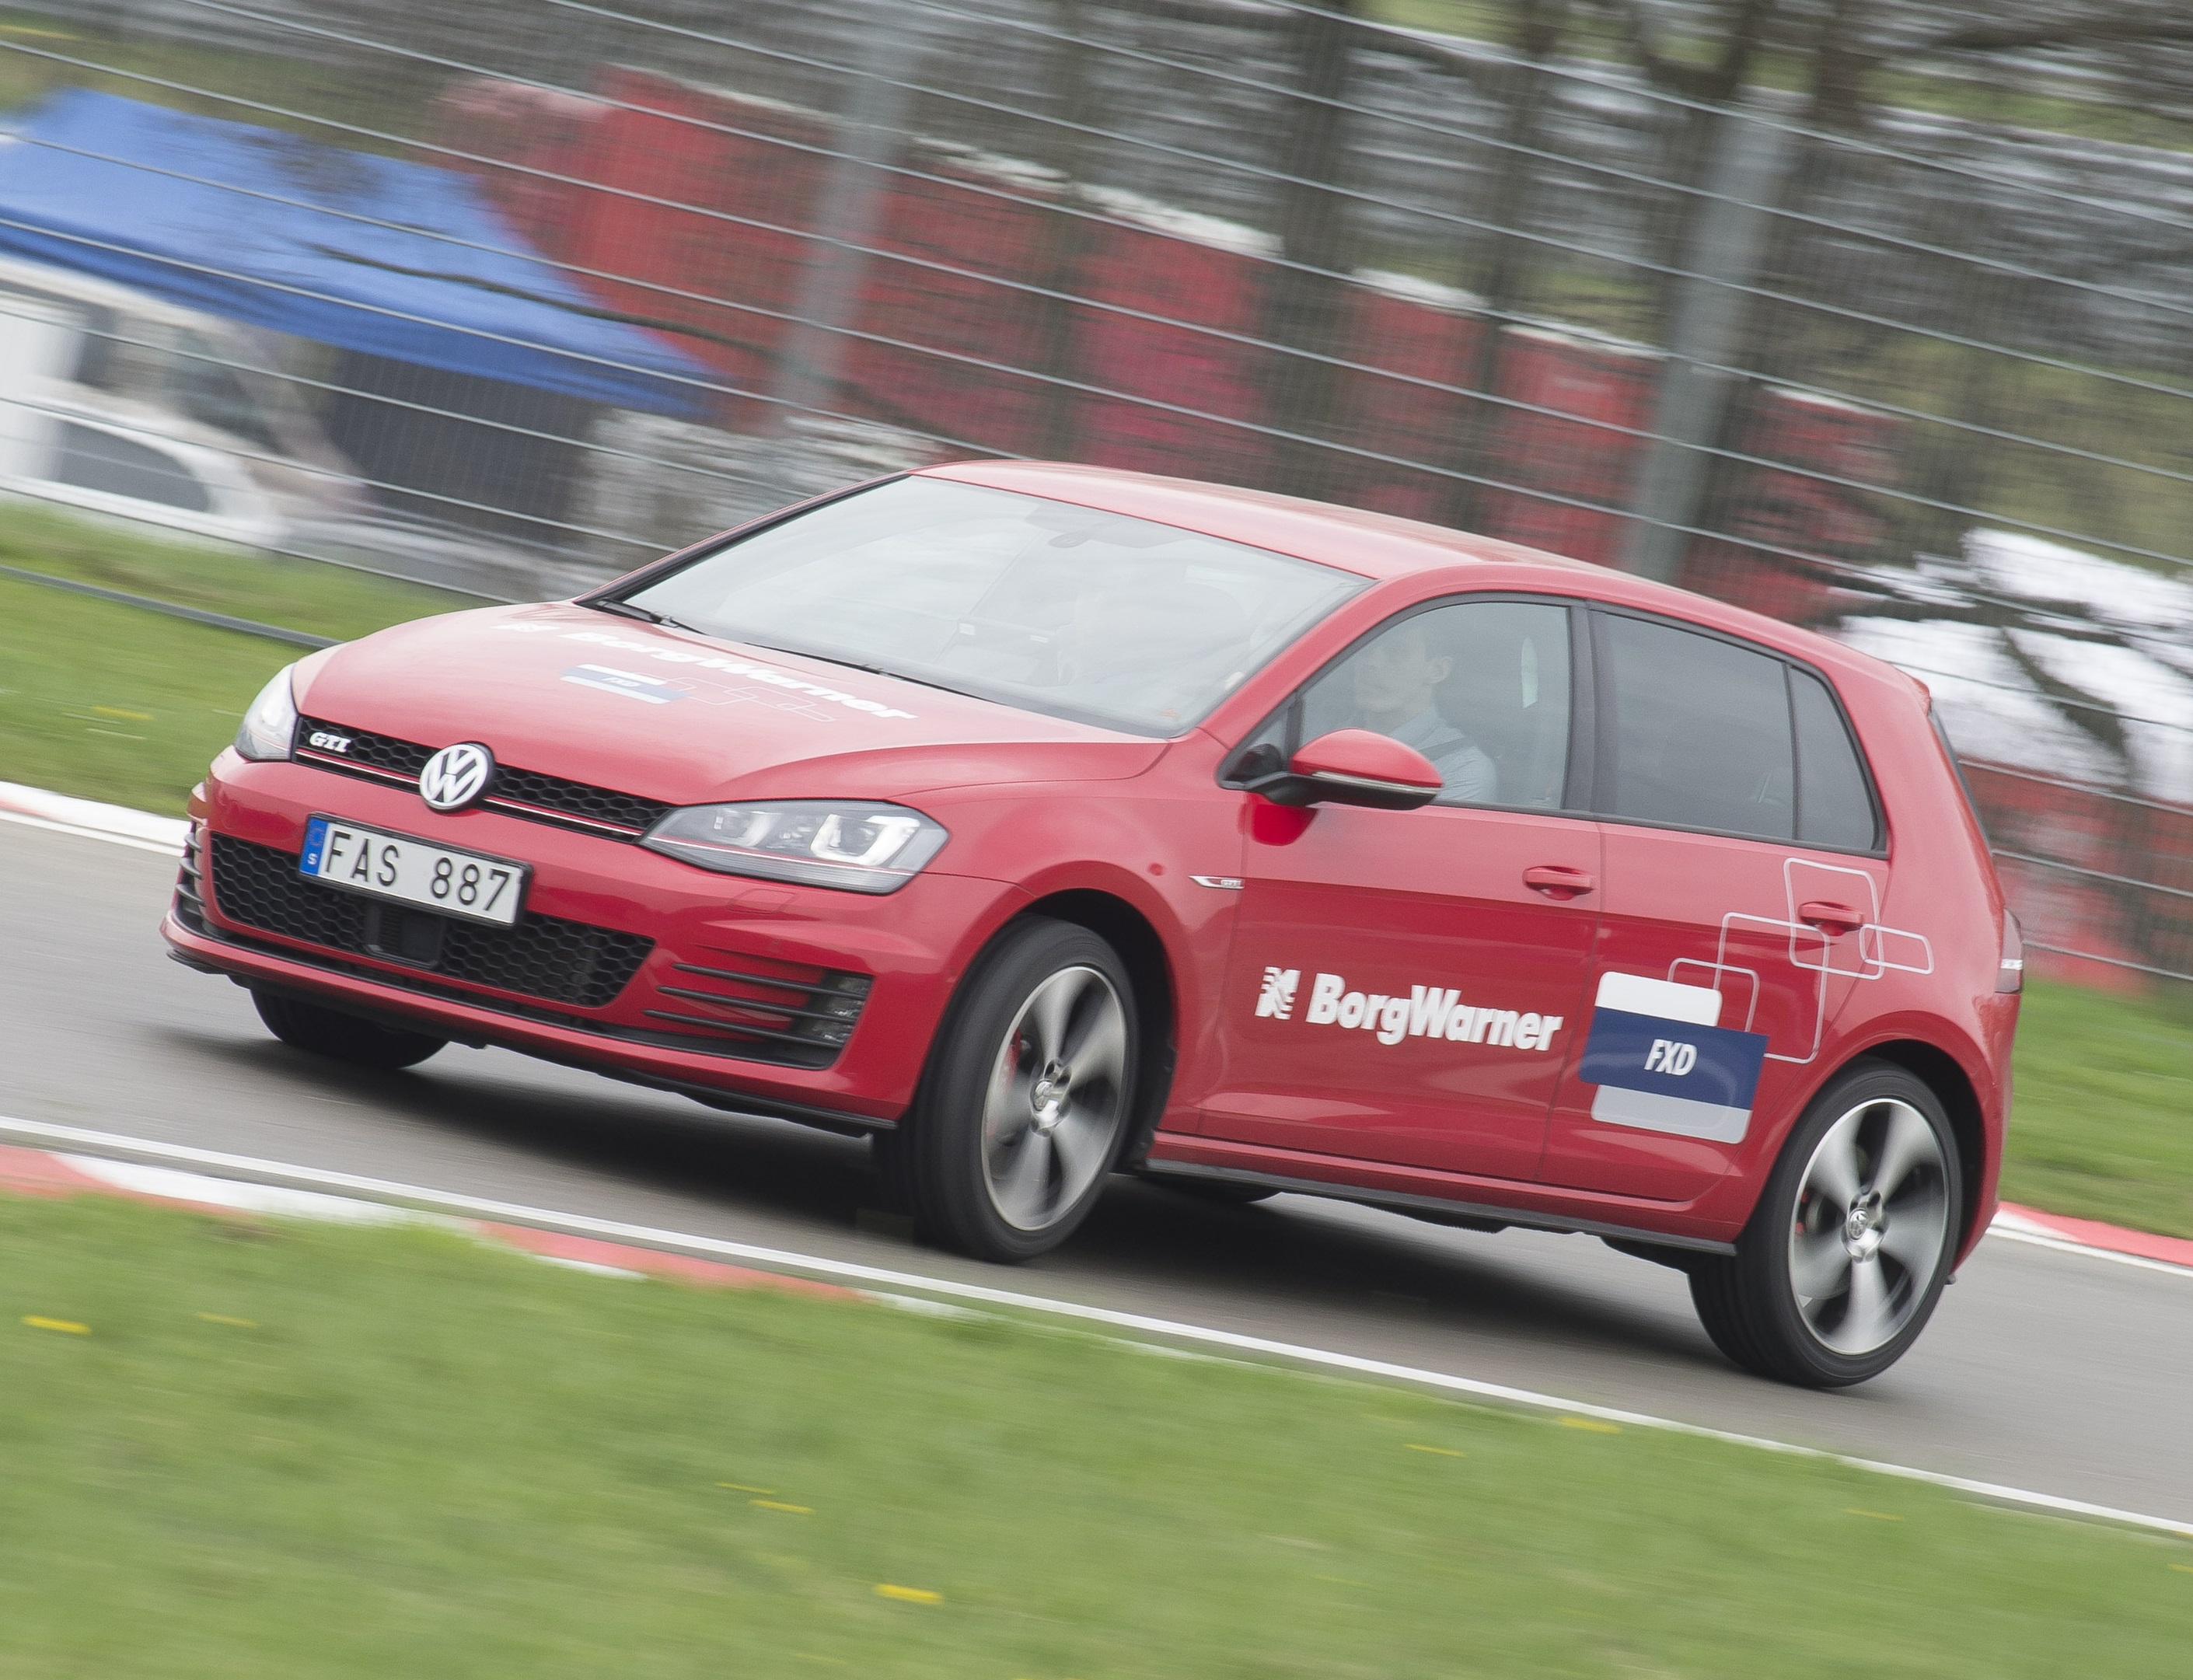
\includegraphics[width=1\textwidth]{Pictures/golf}
	\caption {Golf GTi Mk7 equipped with FXD.}
	\label{golf}
\end{figure}
 % Introduction

\chapter{Theory}

Before describing the work on friction estimation it is important to have some knowledge within vehicle dynamics, including basic knowledge on how tires and also different differentials work. The following chapter tries to describe this so that the reader has the right basic knowledge needed.

\section{Vehicle dynamics and models}

When looking at vehicle dynamics, there are many variables that are interesting to know. Some of these include the vehicles yaw rate, and the velocity and force generated in both lateral and longitudinal direction. Some variables can be measured directly and some of them needs to be calculated or modeled. The characteristics of a whole car is very complex and the exact behavior of a car is therefore impossible to model in every situation. There exists many different car models that try to describe the characteristics of a car as adequate as possible. All the calculations for these models are to be done on a cars on board computer, which means that the model has to be simple enough to not reach the computers limited computing capacity.

\subsection{The bicycle model}

The bicycle model is a rather simple model that can be used to describe vehicle dynamics when turning, e.i. when we have a yaw rate and lateral forces that are affecting the vehicle. The models major simplifications are that the mass of the car is seen as one center of gravity point and that the two front wheels and the two rear wheels are combined into one wheel respectively as can be seen in Figure \ref{bicycle_model}. These simplifications means that there is no difference in forces on the two sides, e.i. there will be no roll effect to the outside wheel when turning in a corner. There is also an assumption made that there will be no pitch effect on the car, which means that there is no suspension system that is effecting the car. The model also assumes that there is no driving torque generated to the wheels, and therefore only lateral forces on the vehicle.

For most cornering situations, these assumptions work fine, and the model gives a good idea on how different parameters are affected. Despite this, one has to bare in mind that these assumptions could result in rather large errors during certain driving situations.

\begin{figure}[h]
	\centering
	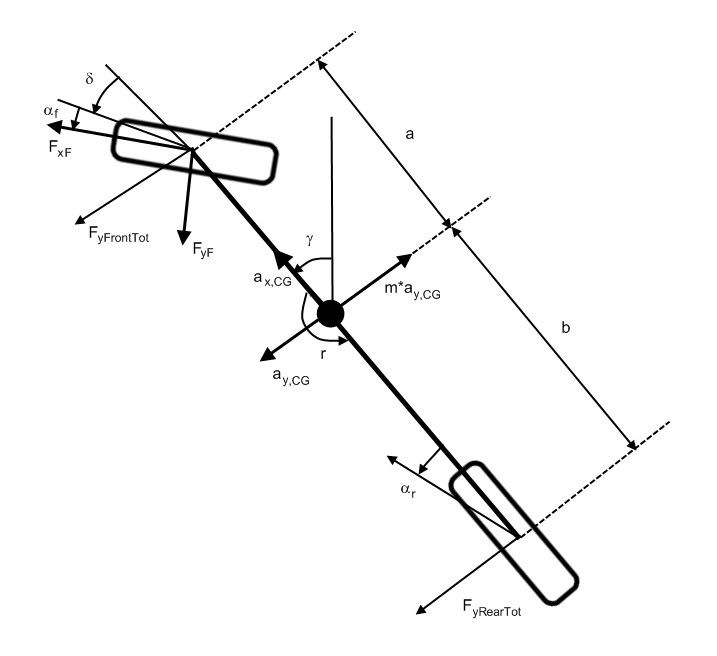
\includegraphics[width=0.8\textwidth]{Pictures/bicycle_model}
	\caption {Bicycle Model. \cite{fordonsdynamik99}}
	\label{bicycle_model}
\end{figure}

The total lateral force acting on the car will depend on the combined forces that the front and rear tires contribute. By using Newtons second law of physics, $ F_{y} = m*a_{y} $, the total lateral force acting on the car will be:
\begin{equation} \label{eq:lateral_force}
	F_{y} = m \cdot a_{y} = F_{yR} + cos(\delta) \cdot F_{yF} + sin(\delta) \cdot F_{xF} 
\end{equation}
where $ m $ denotes the vehicle mass, $ \delta $ is the front wheel steering angle. The acceleration in the center of gravity can be described as: 
\begin{equation} \label{eq:lateral_acceleration}
	a_{y} = \dot v_{y} + \dfrac{F_{c}}{m}
\end{equation}
where $ \dot v_{y} $ is the actual change of velocity in lateral direction and the centripetal force in the center of gravity, $ F_{c} $, depends on the yaw rate:
\begin{equation} \label{eq:yaw_rate}
	\dot \psi = \dfrac{v_{x}}{R}
\end{equation}
\begin{equation} \label{eq:centripetal_force}
	F_{c} = \dfrac{m \cdot v^2_{x}}{R} = mv_{x}*\dot \psi
\end{equation}
where $ R $ is the radius of the turn and $ v_{x} $ the velocity in the direction that the car is pointing. By combining Equations \ref{eq:lateral_acceleration} and \ref{eq:centripetal_force}, the acceleration can described as:
\begin{equation} \label{eq:lateral_acceleration_2}
	a_{y} = \dot v_{y} + v_{x}*\dot \psi
\end{equation}
When combining Equations \ref{eq:lateral_acceleration_2} and \ref{eq:lateral_force} the three different lateral force components that are effecting the vehicle can be described as:
\begin{equation} \label{lateral_forces_2}
	F_{yR} + cos(\delta) \cdot F_{yF} + sin(\delta) \cdot F_{xF} = m*(\dot v_{y} + v_{x} \cdot \dot \psi)
\end{equation}
If taken one step further, the lateral force components can describe the torque created around the z-axis in the center of gravity: 
\begin{equation} \label{yaw_bicycle}
	M_{z} = I_{z} \cdot \ddot \psi = a*(cos(\delta) \cdot F_{yF} + sin(\delta) \cdot F_{xF}) - b \cdot F_{yR}
\end{equation}
where $ a $ and $ b $ are the lever lengths from the center of gravity to the front respective the rear axle and $ \ddot \psi $ the yaw acceleration. 

When looking at the bicycle model, the assumption is that the longitudinal force is negligible. This means, as mentioned earlier, that the lateral force will almost only depend on the tire slip angle created by the front wheel steering angle and the angle to the direction the front wheel is heading towards. When assuming this model with only two wheels, the slip angles for the front respective rear tires will be:
\begin{equation} \label{eq:wheel_slip_front}
	\alpha _{F} = -arctan(\dfrac{v_{y} + \dot \psi  \cdot a}{v_{x}}) + \delta
\end{equation}
\begin{equation} \label{eq:wheel_slip_rear}
\alpha _{R} = -arctan(\dfrac{v_{y} - \dot \psi  \cdot b}{v_{x}})
\end{equation}
This angle is defined to be the angle between the direction of the tire and the direction of the velocity of the wheel. A number of interpretations can be made from these formulas. One is that the steering angle only directly influences the slip angles of the front wheels. Another is that if the numerator in \ref{eq:wheel_slip_front} goes to zero, which means that the lateral velocity plus the yaw rate is zero, the slip angle of the front wheel is equal to the front wheel steering angle. This means that the vehicle is gliding straight forward regardless of the steering angle. Another conclusion is that if $ \dot \psi *b $ is larger than $ v_{y} $, in \ref{eq:wheel_slip_rear}, the numerator will become less then zero and slip angle of the rear wheel will move to the other side on the x-axis. This happens when a vehicle takes a corner more aggressively, which means higher longitudinal velocity compared to the radius of the corner, leading to higher yaw rate as can be seen earlier in \ref{eq:yaw_rate}.

The lateral forces acting on the front and rear wheels can also be described as: 
\begin{equation}
	F_{yF} = 2C_{F}\alpha _{F}
\end{equation}
\begin{equation}
	F_{yR} = 2C_{R}\alpha _{R}
\end{equation}
where $ C_{F} $ and $ C_{R} $ are the lateral force coefficients for one front respective rear tire. The above calculations are taken from \cite{rajamani}. A steering response, $ B $, can de defined from these two forces \cite{fordonsdynamik99}:
\begin{equation}
	B = F_{yR} - F_{yF}
\end{equation}
If $ B $ is 0, we have equal amount of lateral force on the front and rear wheels, which means that there is no under- or oversteer. Theoretically, this means that with a constant steering angle, the radius of the corner will be the same for all velocities. With a $ B < 0 $, a car has more force on the front tires, leading to that less and less steering angle is needed when the velocity increases in a corner. At one point, the steering angle will have to be negative to keep the radius of the corner. This phenomena is called understeer. If $ B > 0 $ on the other hand, more force will be on the rear tires and more steering angle is needed to keep the radius of a corner when increasing the velocity. This kind of behavior is called understeer. A slight understeer is usually desired for commercially available cars because handling of the car becomes easier and the risk of skidding is reduced.

\subsection{Two track vehicle model}

The bicycle model described earlier is a simplified car model that only captures the main characteristics well in many situations. The fact that it is modeled by only one wheel per axis means that the forces on the two wheels on the same axis will be modeled exactly the same. In reality, there will of course exist factors that affect the two wheels different, e.g. when cornering, the normal force will be transfered from the inner to the outer wheel. If a car uses an FXD, the active differential will in certain situations transfer torque from one shaft to the other. The effect that the FXD contributes with will be described further on in a later section of the paper. A model that is slightly more complicated than the bicycle model,  that tries to capture these lateral differences, is the two track model seen in \ref{two_track_model}. 

\begin{figure}[h]
	\centering
	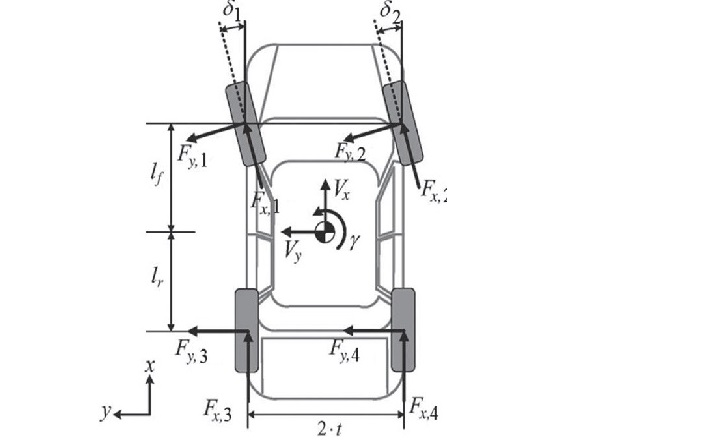
\includegraphics[width=0.8\textwidth]{Pictures/two_track_model}
	\caption{Forces acting on the car with a two track model.}
	\label{two_track_model}
\end{figure}

A couple of assumptions are made in this report when considering the two track model. There will never be a steering angle on the rear wheels and also the steering angle of the two front wheels are considered to be identical. Cars that are using an FXD are exclusively front wheel driven, and therefore the rear wheels will never contribute with positive forces. 



\subsection{Normal forces}
\label{normal_force}

The longitudinal and lateral forces that act on the tires are dependent on the normal forces. It is therefore interesting to know how much normal force that's acting on each tire in order to find out how much longitudinal and/or lateral force the tires can transfer.

\subsubsection{Lateral influence}

\begin{figure}[h]
	\centering
	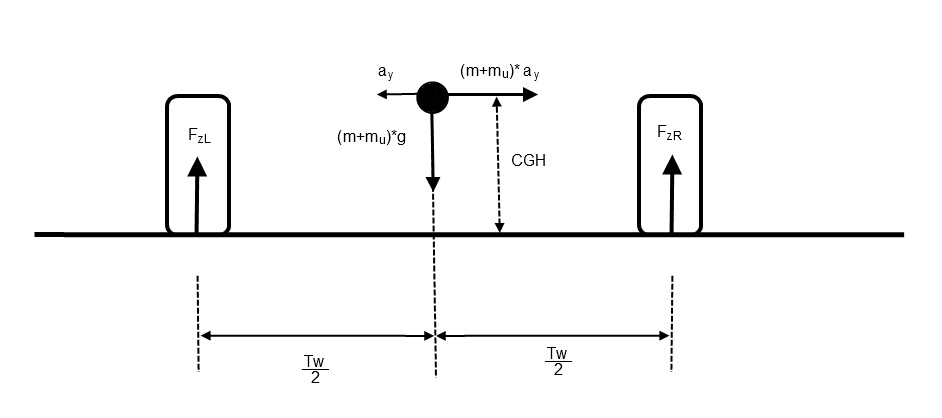
\includegraphics[width=0.8\textwidth]{Pictures/normal_force_lateral}
	\caption{Normal force on the car seen from the front.}
	\label{normal_force_lateral}
\end{figure}
Without any lateral acceleration, the normal forces on the right and left hand side of the car, as seen in Figure  \ref{normal_force_lateral}, can simply be described as:
\begin{equation} \label{eq:normal}
	F_{zL} + F_{zR} = mg
\end{equation}
With lateral acceleration affecting the car, a torque will occur that changes the normal forces on the two sides: 
\begin{equation} \label{eq:normal_with_lat_acc}
	F_{zR}*T_{w} = mg*\frac{T_{w}}{2} + m*a_{y}*CGH
\end{equation}
\begin{equation} \label{eq:normal_with_lat_acc_left}
F_{zL}*T_{w} = mg*\frac{T_{w}}{2} - m*a_{y}*CGH
\end{equation}
$ T_{w} $ is the track width, or distance between the wheels, $ a_{z} $ the lateral acceleration and $ CGH $ the height from the ground to the center of gravity. The torque that is an effect of the lateral acceleration in Equation \ref{eq:normal_with_lat_acc}, does not take into account that the center of gravity height will change during driving.

When taking a corner, there will also be load transfer from the inner to the outer wheel, which will depend on the centripetal force, $ F_{c} = ma_{y} $, and the load transfer coefficient $ \sigma_{i} $.
\begin{equation}
	\Delta F_{zi} = \sigma_{i} ma_{y}
\end{equation}
\begin{equation}
	\sigma_{i} = \frac{1}{T_{w}}*( \frac{c_{\phi i}}{c_{\phi 1}+c_{\phi 2} - mgh'}h' + \frac{l-a_{i}}{l}h_{i}) 
\end{equation}
where the \textit{i} denotes one of the axles (either front or rear), $ c $ the roll stiffness, $ h $ the height from the ground to the axle, $ h' $ the distance from CoG to the roll axis, $ a_{1} = a $ and $ a_{2} = b $.

The final normal force on the front right wheel will be the normal force acting on the two front wheels divided by two, the unsprung mass of that one wheel, and the weight from the load transfer.
\begin{equation}
	F_{zFrontRight} = \frac{F_{zFront}}{2} + m_{UnsprungOneWheel}*g + \Delta F_{zFront}
\end{equation}
The problem with the calculations done above, is that the roll stiffness, $ c_{\phi i} $ of both front and rear axle has to be known. The roll stiffness calculations are taken from \cite{pacejka}.



\subsubsection{Longitudinal influence}

\begin{figure}[h]
	\centering
	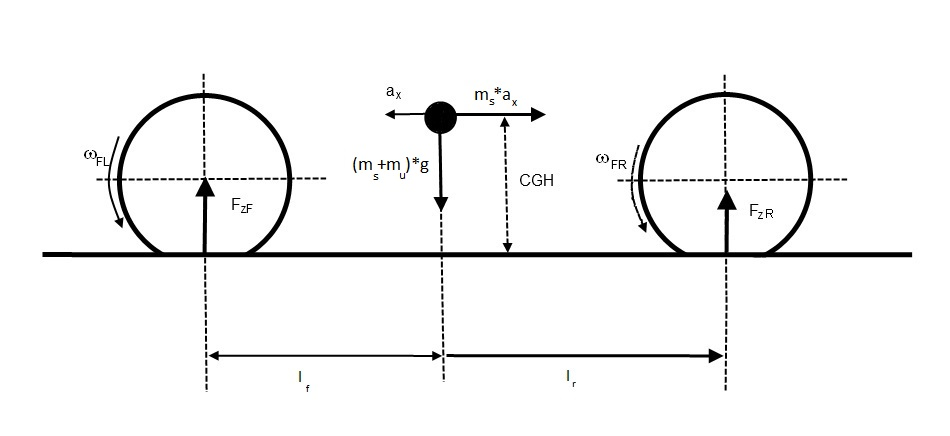
\includegraphics[width=0.8\textwidth]{Pictures/normal_force_longitudinal}
	\caption{Normal force on the car seen from the side.}
	\label{normal_force_longitudinal}
\end{figure}
The normal forces on the front and rear for a vehicle without any acceleration, as seen in Figure \ref{eq:normal_with_long_acc}, is simply the gravitational force acting on the car
\begin{equation} \label{eq:normal_2}
	F_{zF} + F_{zR} = mg
\end{equation}
Note that $ F_{zF} $ denotes the normal force of the rear and not the right hand side like in the previous section. With longitudinal acceleration, the normal forces on the on the front respective the rear will change
\begin{equation} \label{eq:normal_with_long_acc}
	F_{zF}*(a+b) = mg*b - m*a_{x}*CGH
\end{equation}
where $ a $ and $ b $ are the distances from the front and rear axles to the center of gravity. As can be seen in equation \ref{eq:normal_with_long_acc}, he normal force on the front axle will decrease with positive longitudinal acceleration. 

\section{Tire dynamics}
A gas inflated tire that is non loaded will have a radius called unloaded radius. When a tire is loaded, and therefore have a normal force acting on it from the road, it will deform against the road creating a contact area. The contact area is proportional to the load, more load gives a larger contact area. The deformation of the tire will lead to a shorter distance between the center of the tire and the road, this is the loaded radius. 

A loaded tires contact area against the road can be divided into two, adhesion area and sliding area (Figure \ref{adh_sliding}). The adhesion area is the part of the contact area that's said to adhere to the road, this means that this part haven't reached the friction limit yet, it can still handle more force without sliding. The sliding area is the area that has reached the friction limit and thus has begun sliding. How this area is divided depends on a number of factors but it can basically be divided into two cases, longitudinal forces and lateral forces which will be explained further on.
\begin{figure}[h]
	\centering
	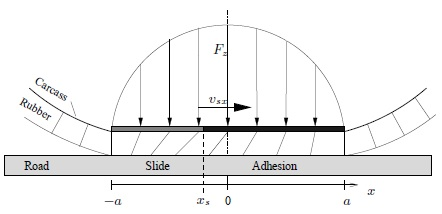
\includegraphics[width=0.8\textwidth]{Pictures/adh_sliding}
	\caption{Adhesion area and sliding area of a tire. \cite{svendenius2013}}
	\label{adh_sliding}
\end{figure}

\subsection{Longitudinal forces}
Rotating the tire will result in compression of the tire where it hits the road and expansion where it leaves the road. The tire itself has a dampening effect meaning that all energy used to compress the tire won't be recovered when it expands again. This energy loss is called rolling resistance, $ F_{rr} $. $ F_{rr} $ is often modeled as being proportional to $ F_{z} $ with the proportionality constant $ f $ (Equation \ref{eq:rollingres}). A typical value of $ f $ is 0.015 for passenger cars \cite{rajamani}. The compression and expansion of the tire will also move the normal force acting on the tire in front of the center line (Figure \ref{rolling_resistance}) when the tire is rolling. The moved normal force will result in a third radius of the tire, the effective rolling radius. This is the radius related to the actual linear longitudinal velocity of the rolling tire, it's longer than the loaded radius but shorter than the unloaded radius.
\begin{equation}
F_{rr} = fF_{z}
\label{eq:rollingres}
\end{equation}
\begin{figure}[h]
	\centering
	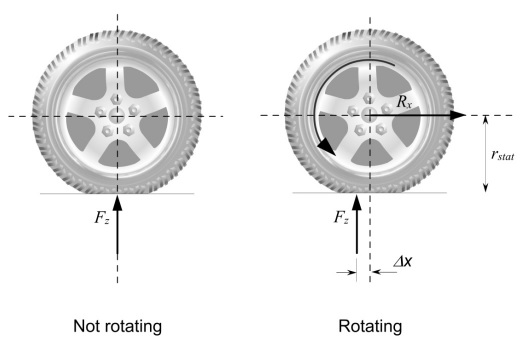
\includegraphics[width=0.8\textwidth]{Pictures/rolling_resistance}
	\caption{Normal force acting on the tire. \cite{rajamani}}
	\label{rolling_resistance}
\end{figure}
Applying torque on the tire will generate longitudinal force moving the tire forwards or backwards. Doing so will always generate a longitudinal slip, called \textit{slip ratio}. This is a ratio of the difference between the angular velocity of the tire and the angular velocity of the corresponding (left or right) undriven wheel. The slip ratio is defined as: 
\begin{equation}
\kappa = \dfrac{R_{e}\omega-V_{x}}{V_{x}}
\label{eq:longslip}
\end{equation}
This leads to the following slip relationships:
\begin{equation}
Locked: \omega = 0 \Rightarrow \kappa = -1
\end{equation}
\begin{equation}
Free rolling: \omega = \frac{V}{R_{e}} \Rightarrow \kappa = 0
\end{equation}
\begin{equation}
Spinning: \omega = 2\frac{V}{R_{e}} \Rightarrow \kappa = 1
\end{equation}
The amount of slip will be one of the factors that decide the ratio between adhesion area and slip area for the tires contact area. The more slip the bigger slip area. The slip area will grow with the slip from the backside of the contact area. When the sliding area is as big as the contact full tire spin occurs. When braking the sliding area will grow from the front and be as big as the contact area when the tire is completely locked. With the same analogy the adhesion area will be as big as the contact area when the tire is free rolling. 

The maximum longitudinal force that can be generated is proportional to the normal force with the friction coefficient as proportionality constant:
\begin{equation}
F_{x,max} =  \mu F_{z}
\label{eq:fxmufz}
\end{equation}
The generated longitudinal force depends on the longitudinal slip. In Figure \ref{fric_slip} the force slip curves for different road conditions can be seen.
\begin{figure}[h]
	\centering
	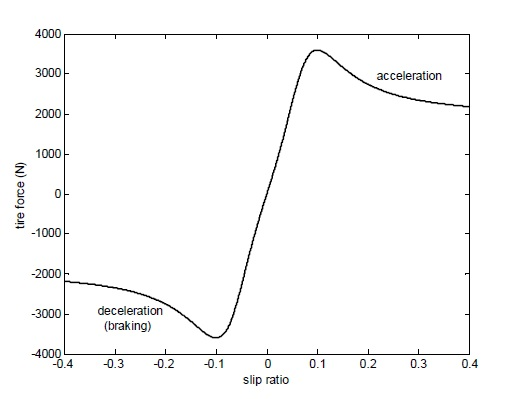
\includegraphics[width=0.8\textwidth]{Pictures/fric_slip}
	\caption{Friction coefficient as a function of slip ratio for a tire. \cite{gustafsson1997}}
	\label{fric_slip}
\end{figure}
The longitudinal force is normalized against the normal force, hence it's the friction coefficient shown on the y-axis. By looking at the graph the characteristics of a tires longitudinal force generation can be seen. For low slips the force curve is linear, at a specific slip a maximum is reached and after that it slowly decays. Different road conditions have different coefficients of friction which is reflected by the different curves maximum values.

\subsection{Lateral forces}
Lateral forces will be generated when the vehicle is turning, more specifically when there is a difference in the angles of the front tires relative the angle of the vehicle. When turned, the tire won't travel in the direction of its orientation, there will be a slip between the tires orientation and the velocity vector. This lateral slip is called \textit{slip angle} since it can be expressed as an angle.

As can be seen in Figure \ref{slipangle_latforce} the lateral force is proportional to the slip angle for small slip angles. For larger slip angles the lateral force converges. In difference to the longitudinal force the lateral force won't decrease for very large slip. This doesn't mean that max steering wheel angle always generates maximum lateral force. In many situations a too large steering wheel angle will over turn the wheel and start decreasing the slip angle hence generating less lateral force.
\begin{figure}[h]
	\centering
	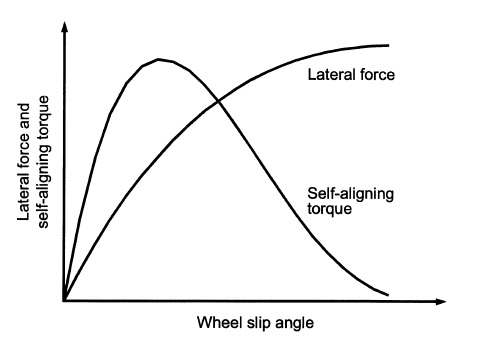
\includegraphics[width=0.8\textwidth]{Pictures/slipangle_latforce}
	\caption{Lateral force as a function of slip angle for a tire. The self aligning torque can also be seen. \cite{sae2004}}
	\label{slipangle_latforce}
\end{figure}

The slip angle is another factor that will decide the ratio between adhesion area and sliding area. When the slip angle is large enough the whole contact area will be in the sliding region, hence the maximum lateral force is generated.

In Figure \ref{slipangle_latforce} the self-aligning torque can also be seen. This is a force generated due to the uneven force distribution over the tires contact area when it's turned. This force increases fast for small slip angles and is the counter force felt in the steering wheel when turning. At a certain point it drops again and this is the locking feeling that's felt in the steering wheel when turning sharp enough.

\subsection{Combined slip}
Since the longitudinal and lateral forces depends on slip ratio and slip angle it's necessary to combine these slips to be able to combine the forces. The total force in any direction can never exceed the normal force times the friction coefficient:
\begin{equation}
F_{total} \leq \mu F_{z}
\label{eq:fmax}
\end{equation}
The total force can be expressed as:
\begin{equation}
F_{total} = \sqrt{F_{x}^{2}+F_{y}^{2}}
\label{eq:ftotal}
\end{equation}
Figure \ref{combined} describes these relations well.
\begin{figure}[h]
	\centering
	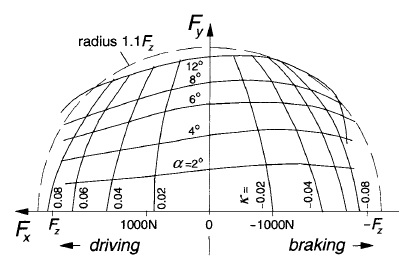
\includegraphics[width=0.8\textwidth]{Pictures/combined}
	\caption{Longitudinal force and slip ratio on the x-axis and lateral force and slip angle on the y-axis. These forces combined can not exceed the circle (Equation \ref{eq:ftotal}) that is the total force expressed as Equation \ref{eq:fmax}. \cite{pacejka}}
	\label{combined}
\end{figure}
It has also been mentioned that both slip ratio and slip angle affects the ratio between adhesion area and sliding area. In analogy with Figure \ref{combined} the sliding areas generated by slip ratio and slip angle will be combined.

\subsection{Tire stiffness}
\label{sec:tire_stiffness}
There are many parameters that needs to be known about the vehicle in order to estimate the friction well. One parameter that is not known (unless specified) is the stiffness of the tires. A tire has two specified stiffnesses, longitudinal and lateral stiffness. The longitudinal stiffness describes how much a tire will deform while being loaded longitudinally, accelerating or braking for example. The vertical stiffness describes how the tire deforms while being loaded vertically, turning for example.

The tire stiffness is a very important parameter to describe how much force a tire can generate. The  force generated from the ground through the tires can, in the linear region, be described as a function of the tire stiffness and the slip. Hence, force generated per slip is proportional to the tire stiffness. Longitudinal and lateral force as functions of stiffness and slip in the linear region:

\begin{equation}
F_{x} = C_{x}*\kappa
\end{equation}
\begin{equation}
F_{y} = C_{\alpha}*\alpha
\end{equation}

Once again it should be stressed that this is only valid in the linear region of the force/slip curves. Thus the theoretical definition of the tire stiffness is the gradient of the force per slip around the origin. 

Different tires can have very different tire stiffness, which of course will have a great impact on the tires performance. Snow tires are much softer than summer tires and are therefore less stiff. Generally, this also means that snow tires reach their maximum generated force at a larger slip than summer tires. In the same way an extra stiff racing tire will reach its maximum force at a smaller slip. The tire stiffness should not have to be set beforehand (meaning that the driver would have to specify if he/she changes tires) and therefore need to be estimated for an accurate friction estimation.


\section{Tire models}
\label{sec:tire_models}
There are several models to describe a tire mathematically. These models can be divided into four categories, empirical models, semi-empirical models, simple physical models and complex physical  models. 

Empirical models describe tire characteristics that are acquired from measurements of the tire. To fit the curve according to measured data the parameters are assessed with methods like regression. A well-known empirical model is the Magic Formula \cite{pacejka}. This model provides good fit for $F_{x}$, $F_{y}$ and $M_{z}$ curves and have coefficients that's easy to interpret.

Models using for example the similarity method are semi-empirical which means that some calculations are replaced by known or measured data. By distorting, rescaling and multiplying the result new relationships are acquired which can describe the tire in different situations. For example one can observe that that the pure slip curves shape doesn't change much \cite{pacejka} when the tire runs on different conditions. By shifting the nominal curve these conditions can be described.

The physical models are purely analytical and aims to describe the tire with the help of its physical characteristics. A simple physical model uses simple mechanical representation and can be calculated fairly easy by hand. This often results in pretty poor accuracy but sometimes that's enough. To get better accuracy a more complex model can be set up and simulated in a computer using aids like the finite element method. 

\begin{figure}[h]
	\centering
	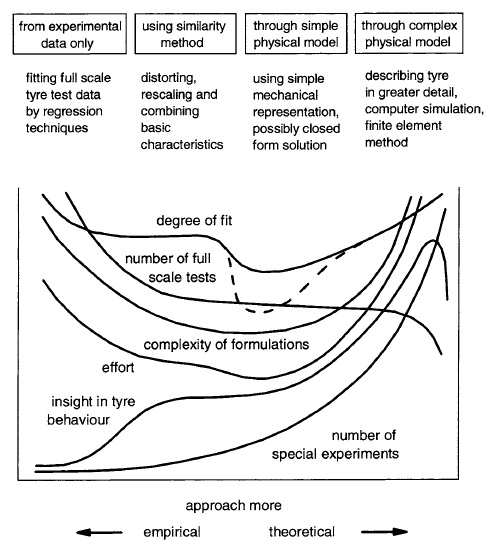
\includegraphics[width=0.8\textwidth]{Pictures/tire_modeling}
	\caption{Four categories of possible types of approach to develop a tire model. \cite{pacejka}}
	\label{tire_modeling}
\end{figure}

In Figure \ref{tire_modeling} some modeling characteristics and how they behave depending on category can be seen.

\subsection{Brush model}
\label{sec:brush}
\todo{insert formula}
The \textit{brush model} is a highly used \textit{simple physical model}. The idea is to model the tire surface as a row of elastic bristles that deflects in different directions depending on how the tire is loaded. This model is illustrated to the left in Figure \ref{brush1}.

\begin{figure}[h]
	\centering
	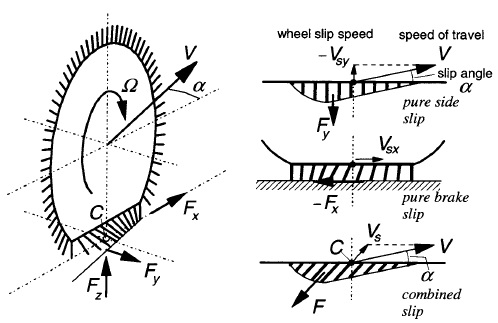
\includegraphics[width=0.8\textwidth]{Pictures/brush1}
	\caption{The brush tire model. \cite{pacejka}}
	\label{brush1}
\end{figure}

For pure side slip the bristles will deflect in the direction of the y-axis, this can be seen at the top right in Figure \ref{brush1}. In the same figure pure brake slip can be seen, that is when the bristles deflects in the direction of the x-axis. Finally at the bottom right of this figure combined slip is illustrated.

\begin{figure}[h]
	\centering
	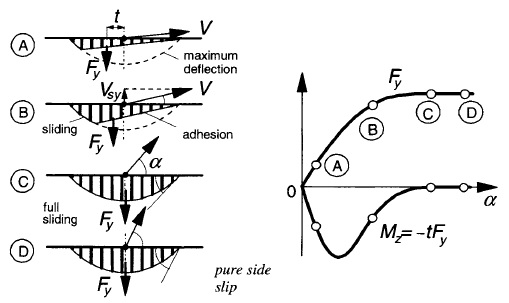
\includegraphics[width=0.8\textwidth]{Pictures/brush2}
	\caption{The brush tire model. \cite{pacejka}}
	\label{brush2}
\end{figure}

In Figure \ref{brush2} it can be seen how different slip angles affects the tire. Small slip angles gives a large adhesion area (flat part) and a small sliding area (curved part). As the slip angle increases a larger number of bristles reaches their maximum deflection, hence increasing the sliding area. At a certain slip angle all bristles have reached their maximum deflection and this results in full sliding. 

\subsection{The Magic Formula tire model}

The magic formula is a series of tire design models developed by H. Pacejka \cite{pacejka} in collaboration with Volvo. The formula is a well known empirical model which has been given its name due to no physical basis for the structure of the equation. It models the fact that different tires has various characteristics which influence the final force generated from the contact patch to the ground. The formula is very complex, where numerous parameters for each tire can be used to calculate lateral and longitudinal forces and also self aligning torque depending on the slip angle or slip ratio. In this report, the magic formula is kept fairly simple to show the idea behind the model, rather than getting a profound understanding behind the development of the model.


\begin{figure}[h]
	\centering
	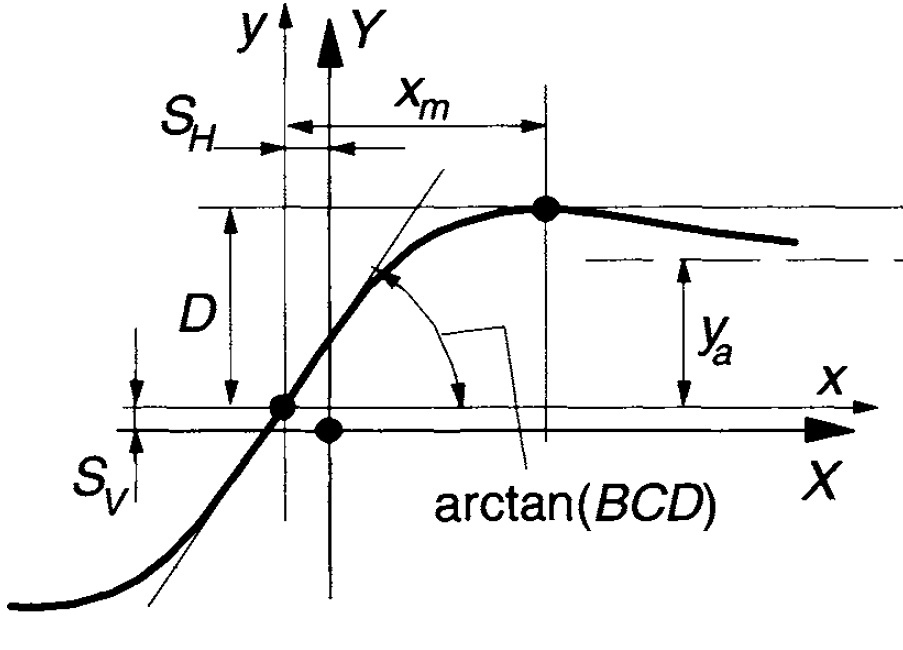
\includegraphics[width=0.8\textwidth]{Pictures/magic_formula}
	\caption{The parameters influence on the magic formula. \cite{pacejka}}
	\label{magic_formula}
\end{figure}

The formula is defined as:
\begin{equation}
	y = Dsin[CarctanBx-E(Bx-arctanBx)]
\end{equation}
where the four fixed constants are:
\begin{itemize}
	\item $ B $ is the stiffness factor.
	\item $ C $ is the shape factor.
	\item $ D $ is the peak factor.
	\item $ E $ is the curvature factor.
\end{itemize}
$ y $ is the output, either lateral or longitudinal force, dependent on $ x $ which is the slip angle, $ \alpha $, or slip ratio, $ \kappa $. The input and output can be affected by a offset, $ S_{V} $ and $ S_{H} $, so the curve doesn't pass through the origin.
\begin{equation}
	Y(X) = y(x) + S_{V}
\end{equation}
\begin{equation}
	x = X + S_{H}
\end{equation}
The stiffness factor, $ B $, depends on the cornering stiffness, $ C_{F\alpha} $:
\begin{equation}
	B = \dfrac{C_{F\alpha}}{CD}
\end{equation}
\begin{equation}
	C_{F\alpha} = c_{1}sin(2arctan(\dfrac{F_{z}}{c_{2}}))
\end{equation}
where $ c_{1} $ and $ c_{2} $ is the maximum cornering stiffness respective the load at maximum cornering stiffness.

D is the maximum lateral or longitudinal force:
\begin{equation}
	D = \mu F_{z}
\end{equation}
The shape and curvature factors can be described as:
\begin{equation}
	C = 1 \pm (1 - \dfrac{2}{\pi}arcsin\dfrac{y_{a}}{D})
\end{equation}
\begin{equation}
	E = \dfrac{Bx_{m} - tan{\dfrac{\pi}{2C}}}{Bx_{m} - arctan(Bx_{m})}
\end{equation}
Where $ x_{m} $ is the distance on x-axis from $ x_{0} $ to the peak of the curve. And $ y_{a} $ is the distance on the y-axis from $ y_{0} $ to the point that the curve converges. Look at Figure \ref{magic_formula} for help.
\subsection{Dugoff tire model}
The longitudinal force described by the Dugoff tire model is defined as:

\begin{equation}
F_{x} = f_{i}*\frac{C_{x} \cdot \kappa}{1-\kappa}
\end{equation}
Where:
\begin{equation}
\;\;\;\;\;\;\, f_{i} = \lambda*(2-\lambda) \;\;\;\;\;\;\;\;\; \text{if } \lambda < 1
\end{equation}
\begin{equation}
f_{i} = 1 \;\;\;\;\;\;\;\;\;\;\;\;\;\;\;\;\;\;\;\;\;\;\;\; \text{else}
\end{equation}
\begin{equation}
 \lambda = \mu \cdot F_{z} * \frac{(1-\kappa)}{2 \cdot C_{x} \cdot \kappa}
\end{equation}
The model depends on four parameters; the slip ratio, the longitudinal tire stiffness, the normal force and the tire/road friction coefficient. Assuming that the slip ratio is the only dynamic parameter during driving, means that $ \lambda $ will be smaller than 1 when the slip ratio is small enough. When $ f_{i} = 1 $ the force will only depend on the longitudinal tire stiffness and the slip ratio, meaning that the friction coefficient and normal force has no impact. 

\subsection{Tire model by Ola}

Three different regions. Three parameters describing the curve: max force slip (at $ \mu = 1$), curvation $ Xsi $ and slope at zero slip $ C_{x} $. \todo{fixa}

\section{Differentials}
When driving in a straight line on a road with equal friction for all wheels, both driven wheels will have equal torque and velocity. In this situation a differential wouldn't even be necessary. The differential is needed when the vehicle is cornering. In this situation the different wheels will have different turning radii, thus requiring different angular velocities. This is the general idea behind a differential, to be able to have different angular velocities of the driven wheels. Without a differential it would be very hard to turn the vehicle, especially at low speeds, since equal speed of the wheels prevents the rotating movement happening while turning.

\subsection{Open differential}
The open differential is the classic differential used in most cars today. With an open differential, the torque will always be evenly distributed to the two driving wheels. One wheel can not have higher torque than the other wheel but they can have different angular velocities. This behavior is directly related to the mechanical construction of the open differential which can be seen in Figure \ref{wikidiff}. 
\begin{figure}[h]
	\centering
	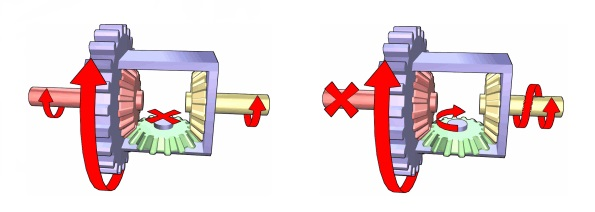
\includegraphics[width=0.8\textwidth]{Pictures/opendiff}
	\caption{The open differential. To the left the case of equal wheel speed, to the right is one wheel completely stationary while the other wheel still rotates. \cite{wikidiff}}
	\label{wikidiff}
\end{figure}
The angular velocities of the two side gears and the crown wheel can be described as:
\begin{equation}
\omega_{r} = \frac{\omega_{1} + \omega_{2}}{2}
\label{eq:diff}
\end{equation}

\subsection{Problems with the open differential}
A situation that creates a problem for a vehicle with an open differential, is when one driven wheel has significant lower friction to the ground than the other. The wheel with low friction can only handle relatively low torque before it starts spinning. This means that the torque applied to the two drive shafts will be restricted by the wheel with the lowest friction to the ground due to the torque splitting nature of the open differential. This will in turn reduce the traction of the car. Two possible scenarios for when the friction to the ground might differ between the driven wheels are when the road is partly covered in ice and when cornering at high speeds which will make the inner wheel lift from the ground. 

When driving on a split-$ \mu $ (different friction coefficients for the driven wheels) surface, the wheel on the low friction area will easily reach maximum force before it starts to spin. The force it can transfer to the ground will thus be the restricted which in turn will restrict the torque applied on the other wheel. The result of all this is that even though only one wheel has bad grip to the ground the traction is still greatly reduced.

The other scenario, when cornering at a high speed leading to the inner wheel lifting, will give the same effect. The normal force acting on the inner wheel will be reduced when it lifts. This will reduce the force that can be transfered to the ground which will reduce the amount of torque that can be applied to the drive shafts. In a worst case scenario the inner wheel has lost contact to the ground completely reducing the transfered force to the ground to zero. The only torque applied is to spin the wheel and this is almost no torque at all compared to the torque used to propel the the car. The propulsive power will be zero and the car will lose speed. After a while the inner wheel will touch the ground again and some force will be transfered only to lift the wheel up again. This will get the car stuck oscillating around this inefficient boundary wasting lots of power.

A solution for these two different scenarios would be to lock the two drive shafts together. This would keep torque applied to the outer wheel even when the inner wheel loses grip, but the fundamental idea of the differential would be lost. That is, the possibility of a speed difference between the two drive shafts. This would also affect the steering behavior in several bad ways, especially at lower speeds. Hence it would be very beneficial to be able to lock the drive shafts together in certain situations. It would be even more beneficial if they were coupled with a device where some slip were allowed between the shafts, making it possible to control the amount of torque transfered from one shaft to the other. Enter, the limited slip differential.

\subsection{Limited slip differential}
The idea of a limited slip differential (LSD) is not to apply more torque to a wheel than it can transfer to the ground. This means that the torque splitting nature of an open differential needs to be countered. Take the sharp turn example from above. The lateral forces of the car will lift the inner wheel from the ground which will result in less traction. With a LSD the torque distribution can be managed so that more torque is applied on the outer wheel. The car will gain more traction when cornering with a LSD than with an open differential. The same effect is applied when driving on a split-$ \mu $ surface. Torque is transfered from the wheel with lower friction to the ground to the wheel with higher friction to the ground to increase the traction.

There are different types of LSDs, they can be divided in two main categories, passive and active LSDs. Passive LSDs are designed in such a way that they do the torque distribution without any required activity from the outside. The Torsen differential is a brilliant example of a passive differential. A complex set of worm gears and spur gears results in a differential that does the torque distribution by itself when needed. Passive differentials require little effort to use but the properties of the differential can't be changed in any way.

Active differentials are controlled from the outside. The amount of torque transfered from one shaft to the other can be freely controlled and this gives much more power over the cars behavior.

\subsection{FXD}
The FXD is an active limited slip differential made by BorgWarner AB for FWD cars. It uses the same clutch technology as their four wheel drive systems. Instead of using the clutch to transfer torque between front and rear it's used to transfer torque between the left and right front wheels. The fact that the clutch is actuated from the outside is what makes the FXD an active limited slip differential, the torque transfered between the wheels is freely controlled.

\subsubsection{The clutch}
The clutch is based on BorgWarner's Gen5 clutch. This is an electro-hydraulic basket clutch. The clutch is engaged by building a hydraulic pressure in the clutch forcing the clutch plates together resulting in a torque transfer. The pressure is built up by a hydraulic pump operated by an electric DC motor. A the quick and exact control nature of the DC motor results in the clutch being very accurate. The amount of torque transfered through the clutch is easily managed with a rather simple electric signal and above all changed can be made very quick. This is positive when used in cars because things happens very fast.

\subsubsection{The differential}
The differential is basically an open differential but with one major difference, the electro-hydraulic clutch. The clutch is installed in a way that makes it possible to couple one of the drive shafts together with the differential housing. This gives the possibility to transfer torque from one shaft to the other in certain situations. One of these situations is when one wheel has less grip than the other wheel, torque can then be transfered to the wheel with the most grip. When cornering hard or driving on a split-$ \mu $ surface the clutch will be engaged allowing for the torque distribution to be altered.

\subsubsection{Control algorithm}
It's been stated that the FXD itself is very easy to control but to get any real function from it needs to be controlled in a smart way. The algorithm controlling the FXD is complex and powerful. It uses several measured signals from the car which it receives via the CAN bus to calculate the best possible amount of torque to transfer at any time while driving. 

\subsubsection{Benefits of the FXD}
The most obvious benefit of being able to distribute torque freely between the driven wheels is used in several ways to create even more benefits. The overall traction of the car when cornering or running on split-$ \mu $ surface is improved to begin with. Since it's an active LSD it's much easier to avoid heavy under steer compared to passive LSDs where the locking torque can't be controlled at any given moment. It's a lightweight alternative compared to AWD to improve traction performance and it can prevent torque steer.

A major safety benefit is the yaw damping feature. Being able to lock the driven wheels together in an avoidance maneuver will make the car less likely to spin out of control since the locked wheels will prevent the car from rotating around its own axle. Another benefit to safety is the fact that it's an active LSD. This means that torque transfer can cease immediately in favor of the ABS and ESP systems when needed. When this need to happen really fast the DC motor operating the hydraulic pump is short circuited which will make it stop instantaneously releasing all pressure on the clutch.  % Background Theory 

%\chapter{To estimate friction}

\section{What is friction?}
Friction is the force that resists one element of material sliding against another. There are several types of friction, one of them is dry friction which resists relative lateral motion of two solid surfaces in contact. Hence dry friction is the force that one must overcome to pull a box along a floor. Dry friction is the friction that's important for this work. Further on dry friction can be divided in two, static friction and kinetic friction. Coulomb friction is a model used to approximate dry friction. It's expressed as:

\begin{equation}
F_{f}\leq\mu F_{n}
\end{equation}

where

\begin{itemize}
	\item $ F_{f} $ is the force of friction, it's parallel to the surface and has a direction opposed the applied net force.
	\item $ \mu $ is the coefficient of friction, different for different surfaces.
	\item $ F_{n} $ is the normal force exerted by each surface on the other.
\end{itemize}

This model provides a threshold for how much force of friction is needed to move an object. As long as the force of friction is less than or equal to the normal force multiplied by the friction coefficient of the two surfaces the object will remain static. How much force that is needed to move an object along a surface is thus decided by two factors, the normal force acting on the object and the coefficient of friction between the two surfaces. When the force of friction gets larger than this threshold the object will start to move, hence leaving the static friction region and entering the kinetic friction region. 

\section{Tire/road friction}


\section{Restrictions}

\begin{itemize}
	\item slip angle paverkar kraften i langsled
	\item Vy ar svart att fa fram
	\item langsaccelerometer finns inte alltid, berakna acc fran bakhjul brusigt
	\item vad hander nar hjulet spinner -> mycket slip, kraften okar ju inte
	\item kraften som kravs for acceleration paverkas av lutning av vag osv.
	\item 
\end{itemize}

\section{Choosing model}
There have been lots of research and model proposals related to friction estimation. Much of the results from this research usually shows that the proposed solution works very good during testing. This is of course because the researchers are trying to solve a problem proposed by them. Their solution might help this work, but it might as well not help at all. The problem proposed in this work is friction estimation for the FXD, hence it's important to think about the aspects of the FXD when choosing a solution and line of work. First of all, cars with FXD are front wheel driven, meaning that there are no longitudinal forces acting on the rear tires when accelerating. Therefore the velocity of the rear wheels can be used as reference speed for the whole vehicle. This can simplify a solution proposed by someone else where for example advanced GPS equipment are used to determine absolute speed. Another aspect that has to be considered is that the FXD is an active limited slip differential, which means that the torque on the right and left hand side will be different in certain situations compared to a car with an open differential. This can complicate a solution proposed by someone else because that solution assumes that the torque is split evenly between the driven wheels. A last, but very important, aspect that has to be considered is that this friction model has to work in a real car. This means that the proposed solution must for example be able to handle signals that aren't perfect due to noise. All of the things stated above and much more must be considered when deciding what model to use and this is a big part of this work.

\begin{equation}
\mu(F_{z})=\mu_{nominal}*(\mu_{max} + (-k)\frac{F_{z} - F_{z_{0}}}{F_{z_{0}}})
\end{equation}

\section{Friction models}

\subsection{Slip-slope friction model}

One friction model that is frequently used and referred to in research papers is the so called slip-slope friction model. The models general idea is that the maximum tire/road friction available can be decided due to its dependency on the slope from the slip-force curve in the linear region. This slip-force curve has the same characteristics as the slip-friction coefficient curve seen in Figure \ref{fric_slip}. 
\begin{equation}
	\dfrac{F_{x}}{F_{z}} = k*\kappa
\end{equation}
Where $ F_{x} $ and $ F_{z} $ is the estimated longitudinal and normal force acting on a tire depending on input values. The slip-slope can be estimated with for example recursive least square fitting.


\subsection{Kalman filter and recursive least squares}
This approach is done in two steps. First the forces on each wheel are estimated with a Kalman filter. Then the tire road friction coefficient is found by fitting a tire model to the estimated tire force. % Experimental Setup

%\chapter{Friction estimation method}

This chapter will describe the chosen method that has been used to estimate the tire/road friction. Different approaches are weighted where a great deal of effort has been put on dealing with the fact that the method should work well in a practical manner, rather than during simulations.

\section{Approach}
The main idea for how to estimate friction is the following. Two models describing the vehicle forces and the tire forces are used. First all parameters for the vehicle model and all parameters for the tire model except the tire/road friction coefficient is calculated. Next, the tire model is fitted to the vehicle model with recursive least square fitting, using the tire/road friction coefficient as fitting parameter, which will give an estimate of the tire/road friction coefficient. Finally, the estimated tire/road friction coefficient is fed back to the tire model to update the system. A flow chart of this method can be seen in Figure \ref{friction_estimator} This approach is true because the forces generated by the tires should be equal to the total force acting on the vehicle.

\begin{figure}[h]
	\centering
	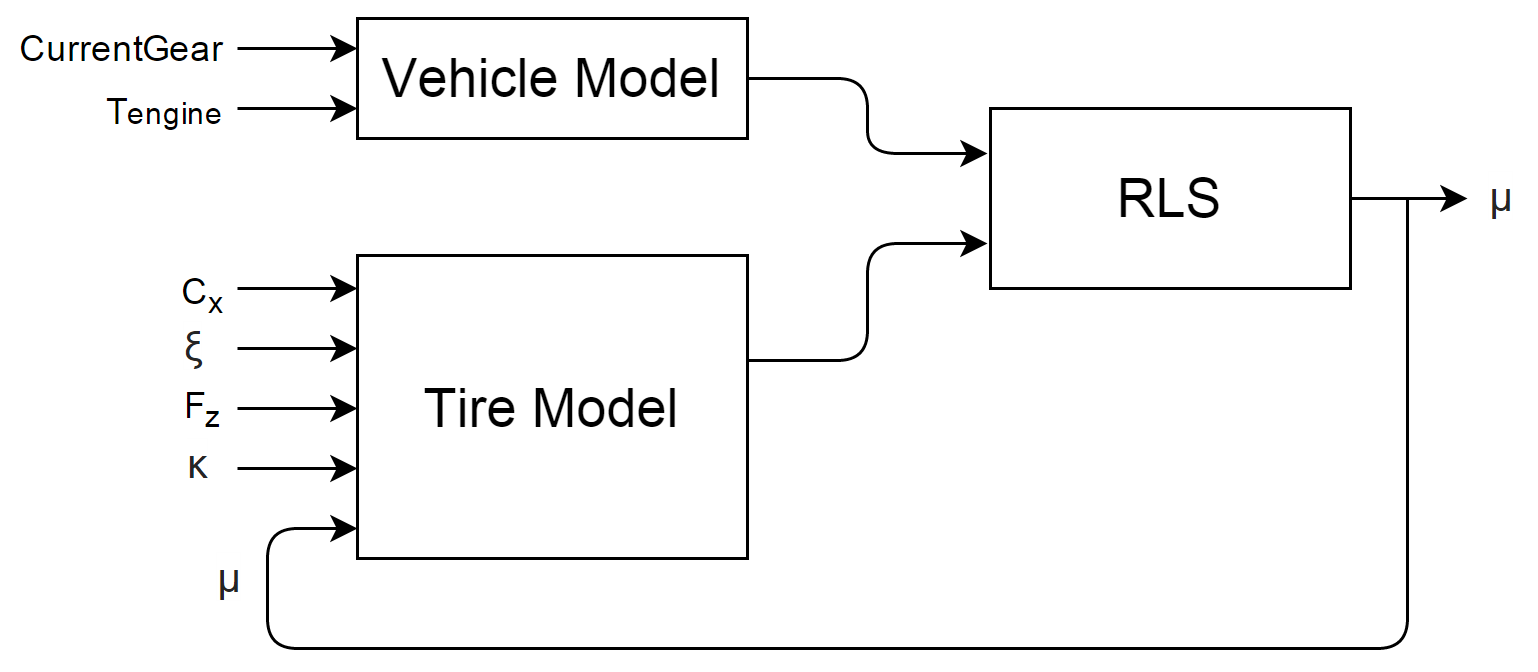
\includegraphics[width=1.0\textwidth]{Pictures/friction_estimator}
	\caption {Simple flow chart of the friction estimator.}
	\label{friction_estimator}
\end{figure}

One of the first parts of method includes calculations of the forces acting on the vehicle by using a vehicle model. This is for example done by using measured and calculated parameters such as wheel speed, yaw rate and acceleration but it can be done in other ways as well. Two different models that describes the vehicle forces will be presented in this work. 

Another part is to calculate the forces generated by the tires through a tire model. Such a model often depend on the tire stiffness, the tires slip ratio, the normal force acting on the tire and the road friction coefficient. Several tire models exists today and in this work four of them is considered. One of them is ruled out almost immediately, two of them is ruled after some more examination and the fourth is the one that is used. More on this later on.

Recursive least square fitting is a well known fitting method with fast convergence and good features such as forgetting factor. This method will be explained in detail as well.

\subsection{Practical restrictions and problems}
The idea presented above might sound like a very simple solution but there are several problems that have to be considered. The most important aspect that has to be taken into account is the fact that the friction estimation model has to work in a real car handled in actual driving situations. In a theoretical world, where a vehicle and a tire model is fed unbiased data, the friction coefficient can be obtained with good certainty and quite fast. Unfortunately, in the practical world, the data fed to the models are far from optimal. Things like measurement noise and approximative calculations corrupts the results. Several more complex driving situations are also hard to model correctly. This can for example be excessive wheel spin, aggressive cornering or speeds close to zero.

The true dynamics of both a vehicle and a tire is very complex and therefore also difficult to describe accurately with a model. At the same time, a model that is to be used has to be simple enough so that calculations are possible on an micro controller unit with limited computational power. Even though many simplified models are shown to be accurate enough to reflect reality in most driving situations, there are times when a simplified model inaccurately describes the detailed dynamics of a vehicle or a tire. 

There are also numerous models that uses parameters which are hard to measure or approximate well in reality. Some of these parameters includes the lateral velocity and slip angle. It is therefore desired to have a model that doesn't rely on these parameters. There are also car specific parameters, some which change between driving sequences, that can have a large impact on the modeled results. A few of these parameters includes the mass of the vehicle, wheel radii, lengths from center of gravity to the rear and front axle and the center of gravity height. The same goes for tires. When changing from winter tires to summer tires the tire stiffness will change a lot which will have a large impact on the results from the tire models. When using simulations, the exact value of these parameters can be known, but in a real environment they either have to be static, approximated or neglected in computations.

\subsection{FXD}
The problem stated in this work is to estimate the tire/road friction for a car using an FXD. This results in a number of conditions that have to be thought of and applied throughout the research. First of all, cars with an FXD installed are solely front wheel driven, meaning that there are no positive longitudinal forces acting on the rear wheels. The velocity of the rear wheels can therefore in most cases be used as a good approximation of the vehicles reference speed. Through the same reasoning, the longitudinal acceleration of the car can be derived from the derivative of the rear wheel velocities. There is also no steering done by the rear wheels.

Another aspect that has to be considered is that the FXD is an electronic limited slip differential, which means that the torque applied to the two driving shafts can differ in certain situations, unlike a car equipped with a standard open differential.

\subsection{Related work}
There have been quite extensive amount of research within this field of study and many different model proposals related to friction estimation during the last decades. The outcome of these researches usually show promising results, where the proposed solution works well during simulations and/or testing. Related work has provided a lot of information and help to this work, especially when it comes to getting a general understanding of the problem and its difficulties. But due to the fact that many results are based on theoretical simulations, a lot of information could be of little use or in some cases even be misleading.

\subsection{Conclusion}
All in all it is a great challenge to estimate the tire/road friction coefficient. \todo{Make sure this is true.} The approach, all of the problems mentioned and how they were taken care of will be explained in greater detail later on in the report.

\section{Signal processing}

Apart from the fact that a vehicle is hard to model properly, there is an uncertainty from the signals taken from the vehicles CAN bus. The true parameter values can be distorted from measuring and process noise as well as being delayed due to calculations and approximations. Different parameter signals can have varying distortions, and therefore include various challenges.

\subsection{Filters}

The signals that are taken from the vehicles CAN bus usually include quite a lot of noise and can cause severe succeeding errors during calculations and approximations. This measure and process noise mainly consist of sudden unwanted changes of the signal that generally has higher frequency than the true parameter value. To exclude these high frequencies, the signal is run trough a low pass filter which will dampen the amplitude of the higher frequencies. The amount of damping for certain frequencies depends on the filters cutoff frequency. 

In Figure \ref{filter_and_no}, the filtered and unfiltered values can be seen for two signals, one of the wheel speeds and the engine torque. It can be seen that the noise of the signals are reduced after filtering, but to a cost of a delaying the signal. The sudden drop of the engine torque, at around $ 11 $ seconds, appears due to a gear change. This sudden drop of engine torque will be seen as a high frequency and is therefore incorrectly suppressed by the low pass filter.

\begin{figure}[h]
	\centering
	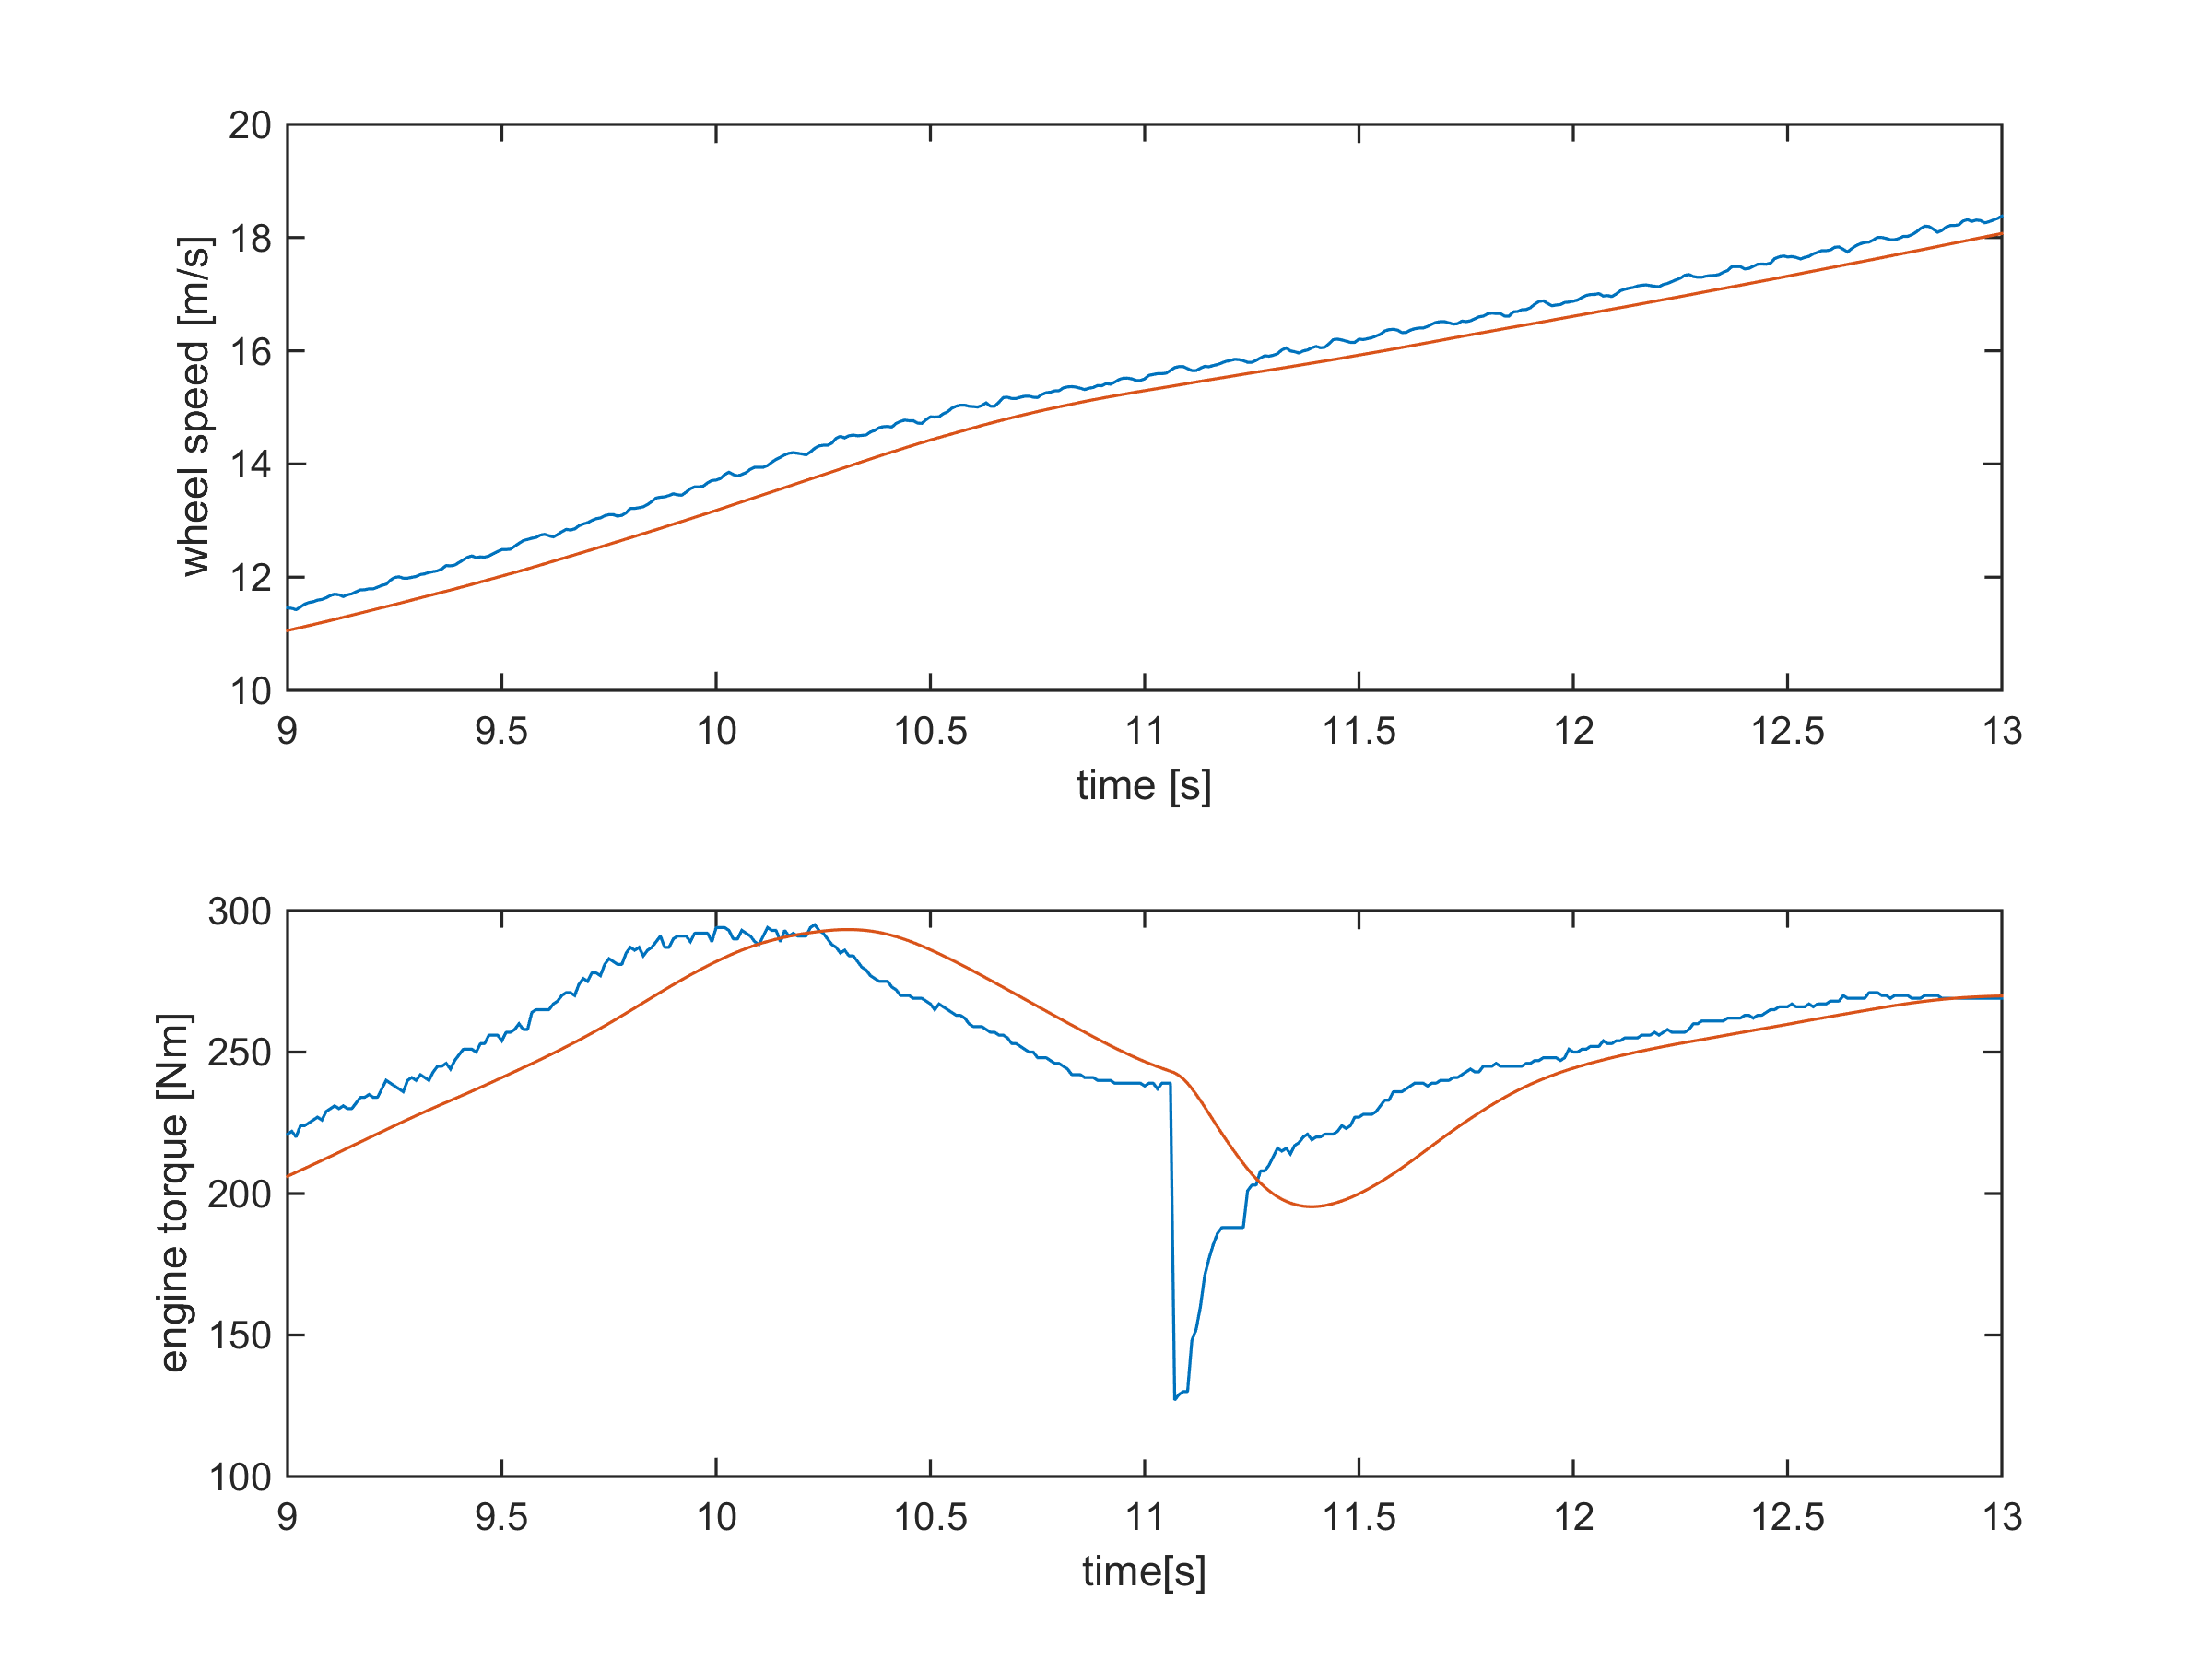
\includegraphics[width=1.0\textwidth]{Pictures/filter_and_no}
	\caption {Wheel speed and engine torque both unfiltered and filtered.}
	\label{filter_and_no}
\end{figure}

The amplitude and frequency of the noise will differ for various signals and could therefore be filtered with different cutoff frequencies to get the most correct value. For example, the engine torque signal, seen in Figure $ \ref{filter_and_no} $, subplot 2, could be filtered with a higher cutoff frequency than the wheel speed, seen in Figure $ \ref{filter_and_no} $, subplot 1, to capture its faster changing characteristic better. However, an important aspect to consider during filtering, is the duration of the delay that will affect the signal. Signals that are run through filters with different cutoff frequencies, will also have differing delay durations. In the extent, this could lead to computations that should equal one another will differ greatly due to their different parameter dependencies. 

In Figure $ \ref{different_filter_val} $, two different force models, that should be equal to each other, are dependent on different parameter values. In subplot one, a signal that affects the tire model is filtered with a cutoff frequency significantly lower than the cutoff frequency for the parameters affecting the vehicle model. In the extent, the force calculated from the tire model becomes delayed compared to the computed vehicle force. In subplot 2 however, the signals are filtered with the same cutoff frequency, hence resulting in a better match between the two models. The conclusion from this is that the low pass filters should not only be designed to get the best possible accuracy for that specific parameter, but the succeeding effects also need to be considered.

\begin{figure}[h]
	\centering
	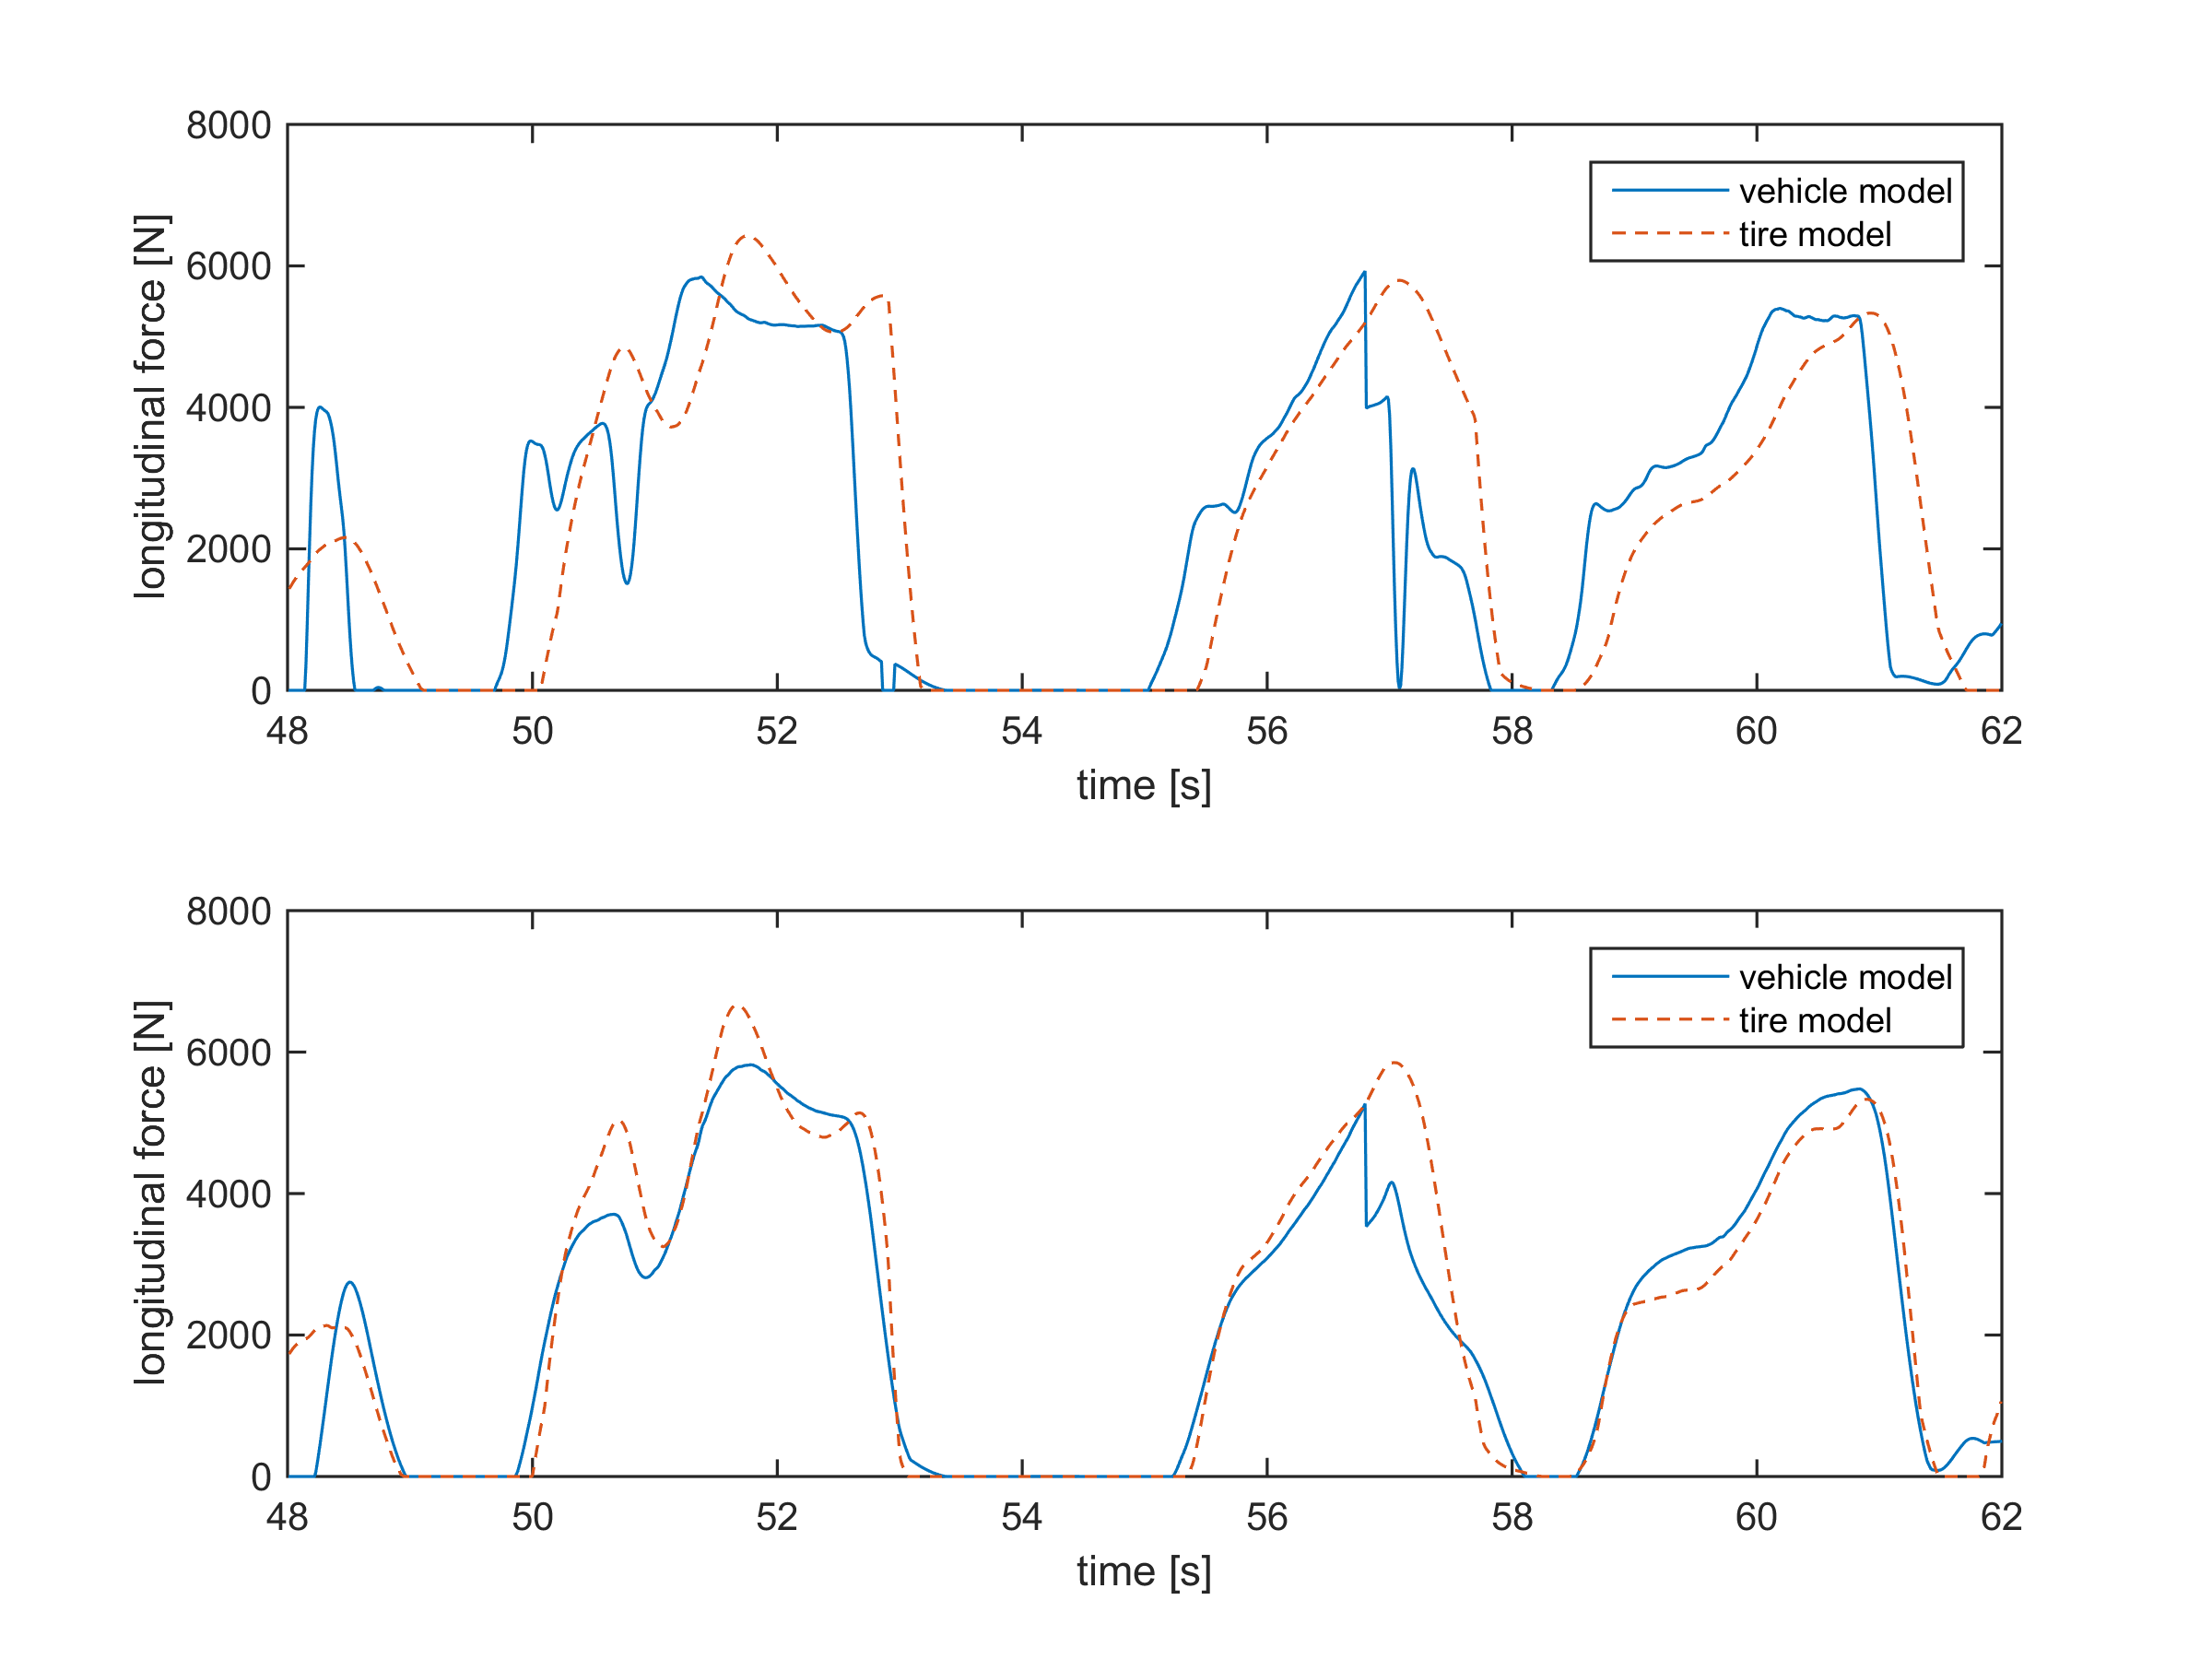
\includegraphics[width=1.0\textwidth]{Pictures/different_filter_val}
	\caption {Vehicle and tire model forces with different filter values for engine torque and wheel speeds.}
	\label{different_filter_val}
\end{figure}

\subsection{Static parameter impact} 
Even if a model can recreate a driving sequence correctly, there will always be an uncertainty due to vehicle specific parameters that are used. Some of these parameters include the position of the CoG, the radius of the wheels and the mass of the vehicle. The position of the CoG will affect the lengths from the CoG to the two axles, denoted $ l_{f} $ and $ l_{r} $ respectively, and also the CoG height from the ground. The position of the CoG will change depending on how the vehicle is loaded. The radius of the wheels can change slightly over time as the tire pressures changes, and can also be different from each tire. The radius of the wheel is used to calculate the velocity of the wheel and also to convert axle torque to force generated at the edge. The mass of the vehicle can change between different driving sequences, depending on how many persons that are seated within the car and also on additional weight. The vehicles mass and CoG height is used to calculate the weigh distribution and therefore also the amount of downward force generated at each tire. 

To get an understanding of how much these parameters affect the result, the force generated from two models with differing parameter values are seen in Figure \ref{force_diff_re_mass}. In the first subplot, the longitudinal force is calculated from a vehicle model that approximates the torque applied to the two driving shafts and thereafter the force generated to the ground by using two different radii. A radius difference of $ 3 $ cm would be very large if considering a tire pressure drop, but could be possible when changing between wheels. In the second subplot, the longitudinal force calculated from a tire model is presented. The two different masses correspond to a vehicle with merely a driver respectively a vehicle with 5 persons. 

\begin{figure}[h]
	\centering
	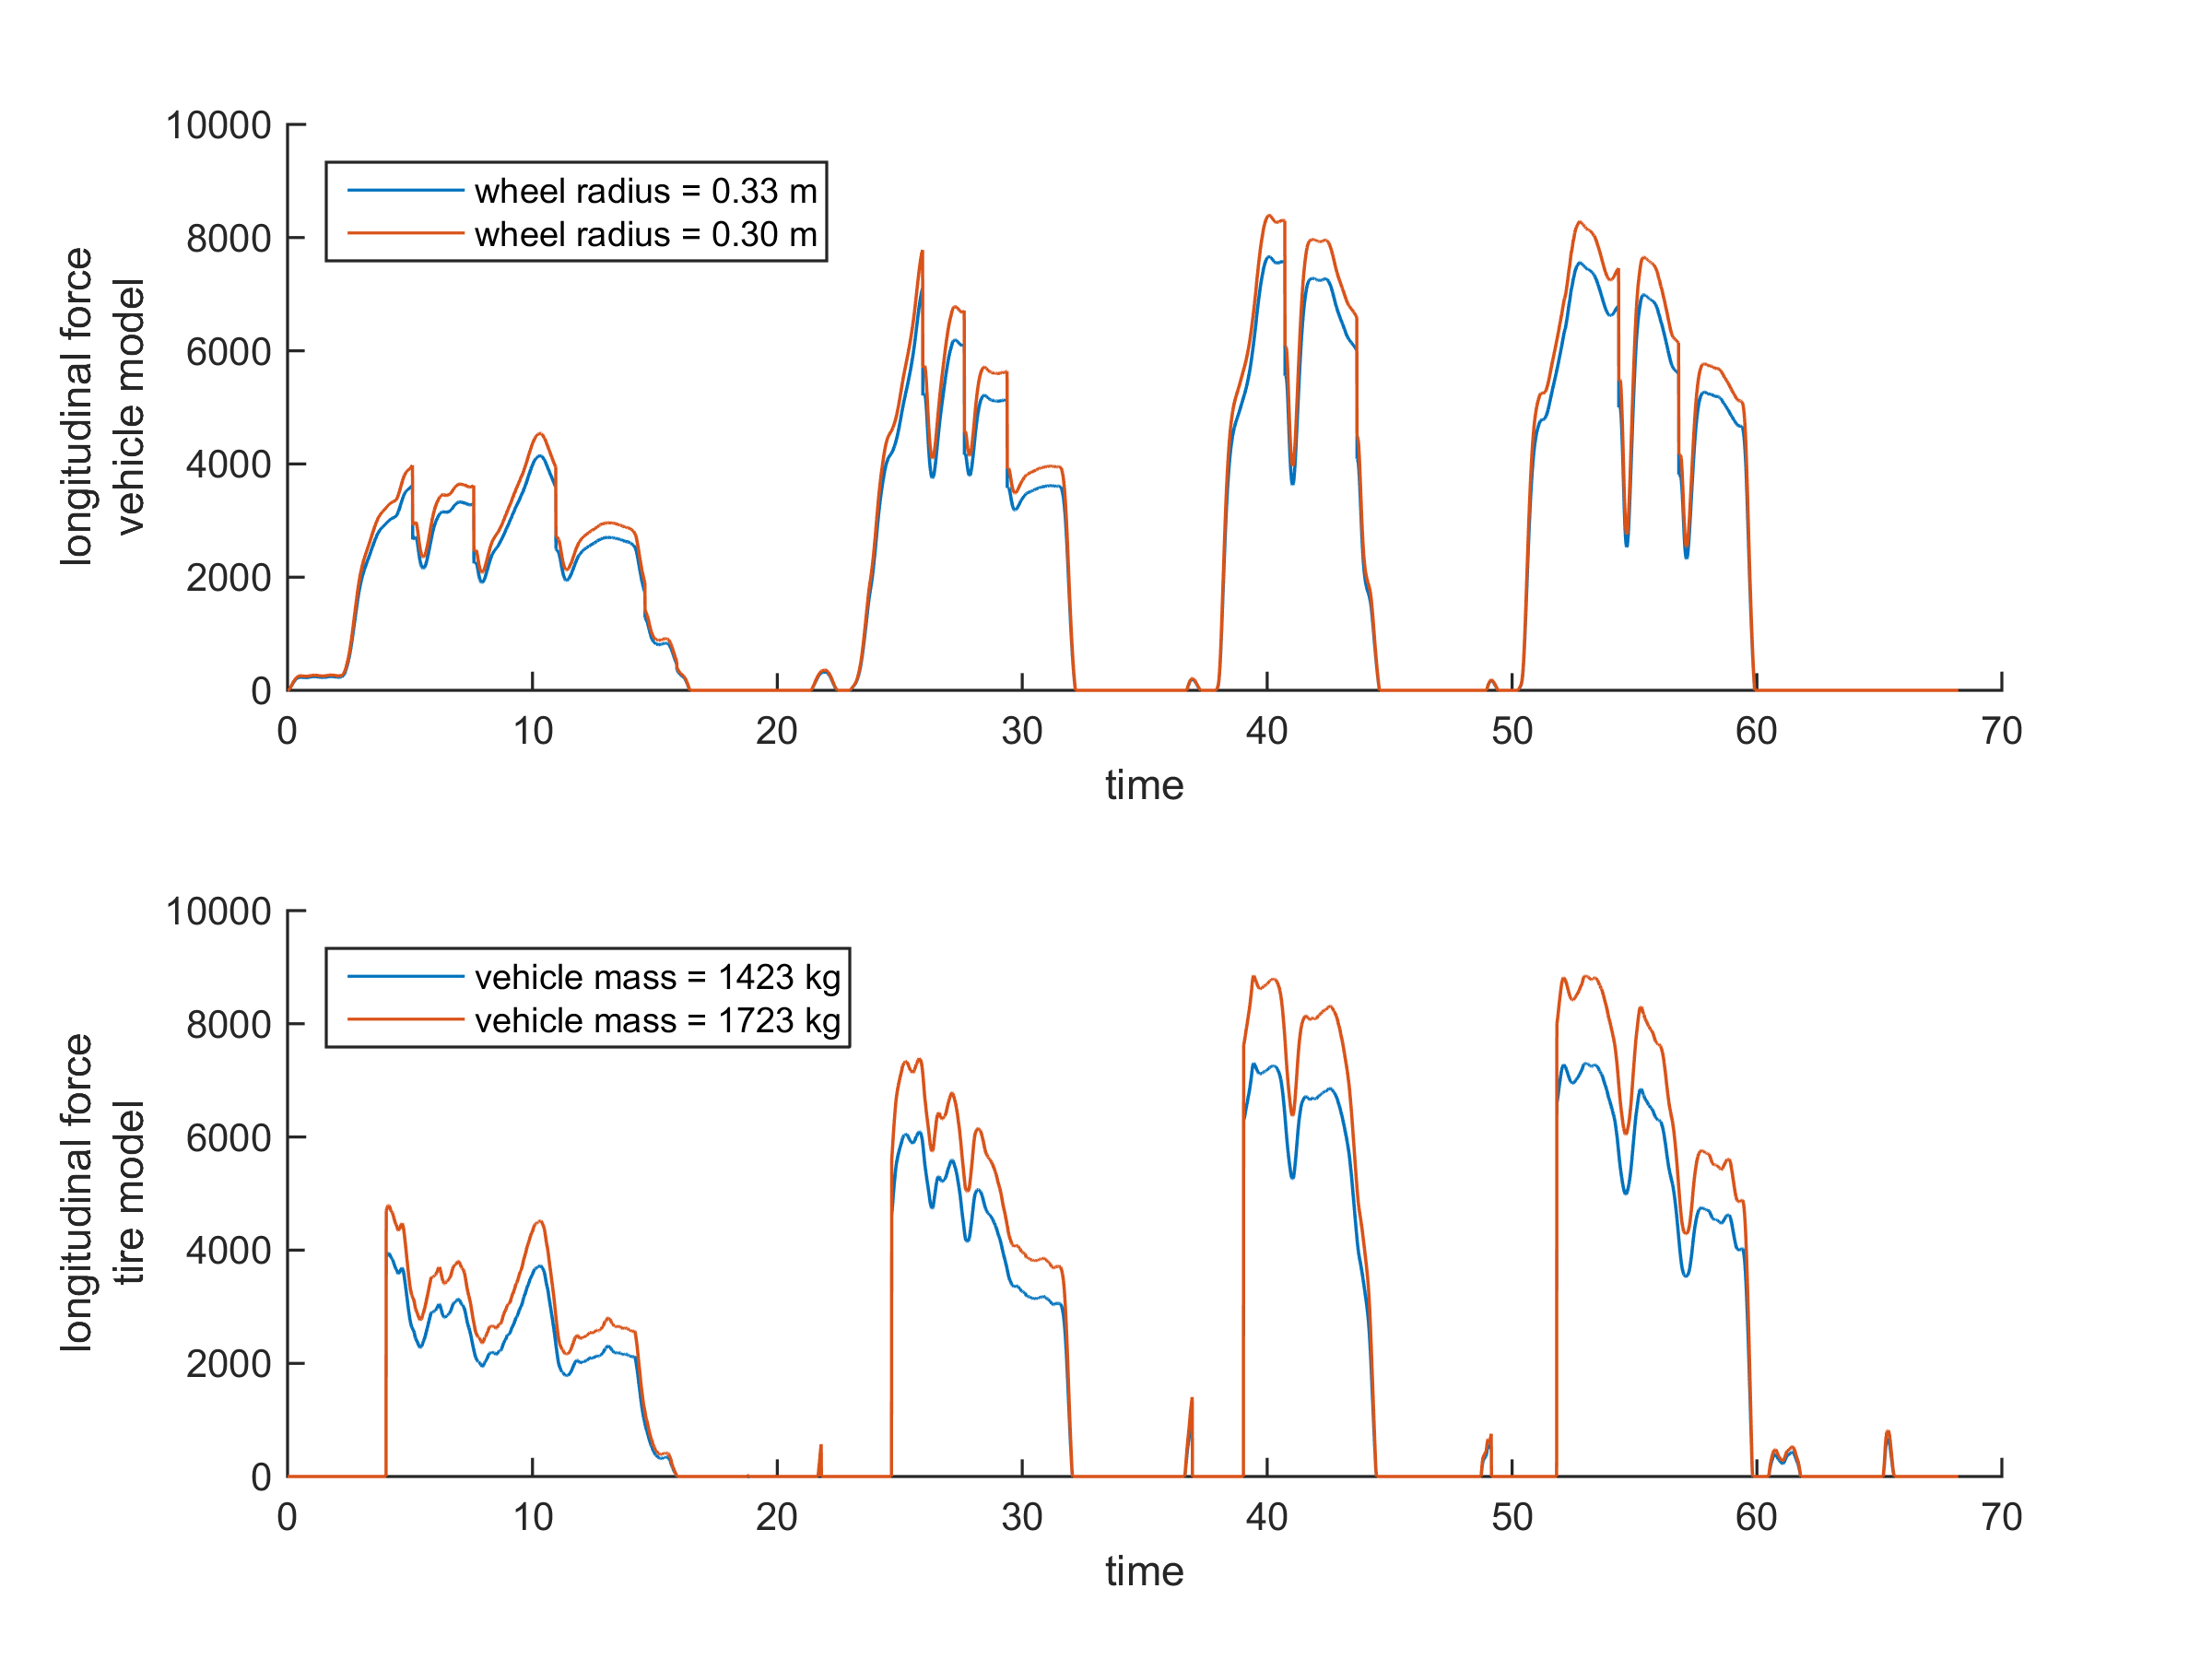
\includegraphics[width=1.0\textwidth]{Pictures/force_diff_re_mass}
	\caption {Forces for different wheel radii and masses.}
	\label{force_diff_re_mass}
\end{figure}

\section{Vehicle forces}
There are several forces acting on a vehicle. The largest forces are generated between the tires and the ground because the tires are the only parts of a car that have any physical contact with the surrounding world. While accelerating and braking longitudinal forces will arise and while cornering lateral forces will arise. The tires are responsible for all the forces that actually control the vehicle which makes them very important for good handling but also makes them hard to model. Beside these major forces there are also forces such as wind drag and rolling resistance acting on the vehicle.

The trick is to calculate all the forces into one total force that can be compared to the total force generated by the tires.
\subsection{Vehicle force calculated from longitudinal acceleration}
The simplest way of representing the force acting on the vehicle while accelerating is to use the acceleration and the mass of the car and apply Newtons second law of motion:
\begin{equation}
	F = m \cdot a
\end{equation}
\subsubsection{Estimating the longitudinal acceleration}
\label{longaccest}
For this method to be accurate an accurate estimation of the longitudinal acceleration is needed. Some cars have accelerometers installed for longitudinal measurements which makes it straight forward to calculate the force. If one of those aren't available the acceleration has to be calculated instead. This can be done by derivation of the vehicles speed. The speed of the vehicle can be obtained by measuring the speeds of the undriven wheels. For a FWD car this would be the rear wheels. To make the calculation more accurate the average speed of the two rear wheels is calculated before the derivation is done.
\begin{equation}
a_{x} = \frac{d}{dt}(\frac{w_{rl}+w_{rr}}{2})
\end{equation}

\subsubsection{Estimating the losses}
Two different losses are compensated for. Losses from drag and losses from rolling resistance.

The drag force is calculated as:

\begin{equation}
F_{D}=\frac{1}{2}\rho v^2 C_{d}A
\end{equation}
where:
\begin{itemize}
	\item $ \rho $ is the density of air.
	\item $ v $ is the speed.
	\item $ C_{d} $ is the drag coefficient.
	\item $ A $ is the cross sectional area.
\end{itemize}
The rolling resistance is calculated as in Equation \ref{eq:rollingres}.

\subsubsection{Estimating the total vehicle force}
The total amount of force acting on the vehicle thus becomes: \todo{this formula might be altered}
\begin{equation}
\label{eq:newton}
F_{vehicle} = m \cdot a + F_{drag} + F_{rolling resistance}
\end{equation}

\subsubsection{Complications}
The main issue with this method is that it's based on longitudinal acceleration and longitudinal losses only, hence it can only be used to estimate the vehicle forces when accelerating in a straight line. Although this is a big restriction it might be enough since acceleration in a straight line happens pretty often while driving.

A major hardship is to obtain a proper value for the longitudinal acceleration. If the vehicle doesn't have an accelerometer the acceleration calculated from the wheel speeds needs to be used. This immediately causes problems when the vehicle is accelerating on a gradient road. During an uphill acceleration, the actual force to accelerate the vehicle will be higher than the force calculated from Newtons second law. Driving downhill, the force will be lower. This is because the earths gravity isn't considered in the formula. When climbing a hill the vehicle force needs to include the force of the earths gravitational pull as well. The same goes for then driving downhill, but now the force will instead help accelerating the vehicle. The force of the gravitational pull can be calculated if the angle of the vehicle relative the earths horizontal plane is known but this angle is hard to measure or estimate. \todo{is it really?} Measuring it with an accelerometer won't work either. The accelerometer will give a better result since the force of gravity is affecting it in some way. This is because it's changing inclination together with the car but it still won't give an acceleration that corresponds to the actual force acting on the car. A solution to this would be to have another accelerometer measuring vertical acceleration of the vehicle but this is extremely uncommon.

The second parameter of Newtons second law is the mass which also is hard to estimate. The mass of the vehicle can vary several hundreds of kilos depending on passengers and load in the trunk. A Golf GTi has a curb weight of about 1350 kg. Hence, the varying weight of several hundreds of kilos will have a great impact on the force calculations. To counter this problem some kind of load detection needs to be available to set a new mass every time the car is driven. This isn't something that is very common on cars today and thus a static mass of the vehicle needs to be set resulting in errors in the force calculations way too often.

Suppose that the force calculation from Newtons second law is correct. Still there are losses to be accounted for. They need to be calculated properly to be able to compare the vehicle force to the tire force. Looking at Equation \ref{eq:newton}, two different losses are compensated for. The rolling resistance is straight forward if the rolling resistance coefficient is known. The drag is a bit more complicated but should prove to be fairly accurate as well if the parameters is known. All in all, the results of these calculations won't be perfect and there are several more losses that can't be calculated in any good way. \todo{are there really?}


\subsection{Vehicle force calculated from engine torque}
Another way of calculating the longitudinal force of a vehicle is to derive the actual torque that is applied to the shafts connected to the driven wheels. The advantage of using the engine torque, instead of the acceleration of the vehicle, is its independence of the roads gradient and losses such as wind drag and steering losses. The torque that is applied to the shafts will be directly proportional to the actual force generated by the wheels, regardless of how the gravitational pull and other losses are acting on the vehicle. 

The formula for calculating the total torque on the drive shafts is simple:
\begin{equation}
\label{eq:tshaft}
T_{driveshafts} = T_{engineshaft}\cdot GearRatio
\end{equation}
where the gear ratio is the speed ratio between the engine shaft and the differential housing:
\begin{equation}
\label{eq:GR}
Gear Ratio = \frac{RPM_{engine}}{RPM_{diffhouse}}
\end{equation}
and finally the speed of the differential housing is the average speed of the left and right drive shafts:
\begin{equation}
\label{eq:diffhouse}
RPM_{diffhouse} = \frac{RPM_{leftdriveshaft}+RPM_{rightdriveshaft}}{2}
\end{equation}
The engine torque, engine speed and the drive shaft speeds (wheel speeds) are all parameters commonly found on the CAN bus of a newer car. Important to notice is that these calculations do not consider any losses from the engine to the drive shaft. By combining Equations $ \ref{eq:tshaft} $ and $ \ref{eq:GR} $, it is seen that the power generated by the engine and the power outputted to the drive shaft are equal.
\begin{equation}
P = T_{driveshaft}\cdot RPM_{driveshaft} = T_{engineshaft}\cdot RPM_{engineshaft}
\end{equation}

The torque will be split evenly between the two drive shafts, assuming an open differential, i.e. when the FXD is inactive. If the FXD is active the available torque on the drive shafts has to the redistributed according to the amount of torque being transfered through the FXD. This is important to consider if force calculations for a single wheel are to be done. 

When the torque on each drive shaft is calculated the force acting on each tire is calculated by dividing that torque by the wheel radius:
\begin{equation}
\label{eq:tireforce}
F_{tire} = \frac{T_{shaft}}{R_{e}}
\end{equation}
These forces can then be compared to the forces generated by the tire models for each tire.

\subsubsection{Gear ratio}
Calculating the gear ratio with Equations \ref{eq:GR} \& \ref{eq:diffhouse} gives varying results. Both the engine speed and wheel speed signals are noisy. In the gear change moment it will take some time for them to stabilize again resulting in long times of faulty force calculations. 

On newer cars it's not very uncommon to find what gear is active at the moment as a signal on the CAN bus. By knowing this the gear ratio can be set without any calculations since the gear ratio for each gear is known. For the Golf GTi the gear ratios can be seen in Table \ref{tab:gr}. A graph of the calculated and predefined gear ratio can be seen in Figure \ref{gear_ratio}. It can be seen that the calculated signal is much slower than the predefined one. It's also oscillating quite much which is bad because the gear ratio really is a static value purely depending on what gear is active. 


\begin{table}[position specifier]
	\centering
	\begin{tabular}{| l | l |}
		\hline
		Gear & Gear ratio \\ \hline
		1 & 13.9284 \\ \hline
		2 & 8.5383 \\ \hline
		3 & 5.4378 \\ \hline
		4 & 3.7206 \\ \hline
		5 & 2.7666 \\ \hline
		6 & 2.1942 \\ \hline
	\end{tabular}
	\caption{Gear ratios for the Volkswagen Golf GTi Mk7}
	\label{tab:gr}
\end{table}

\begin{figure}[h]
	\centering
	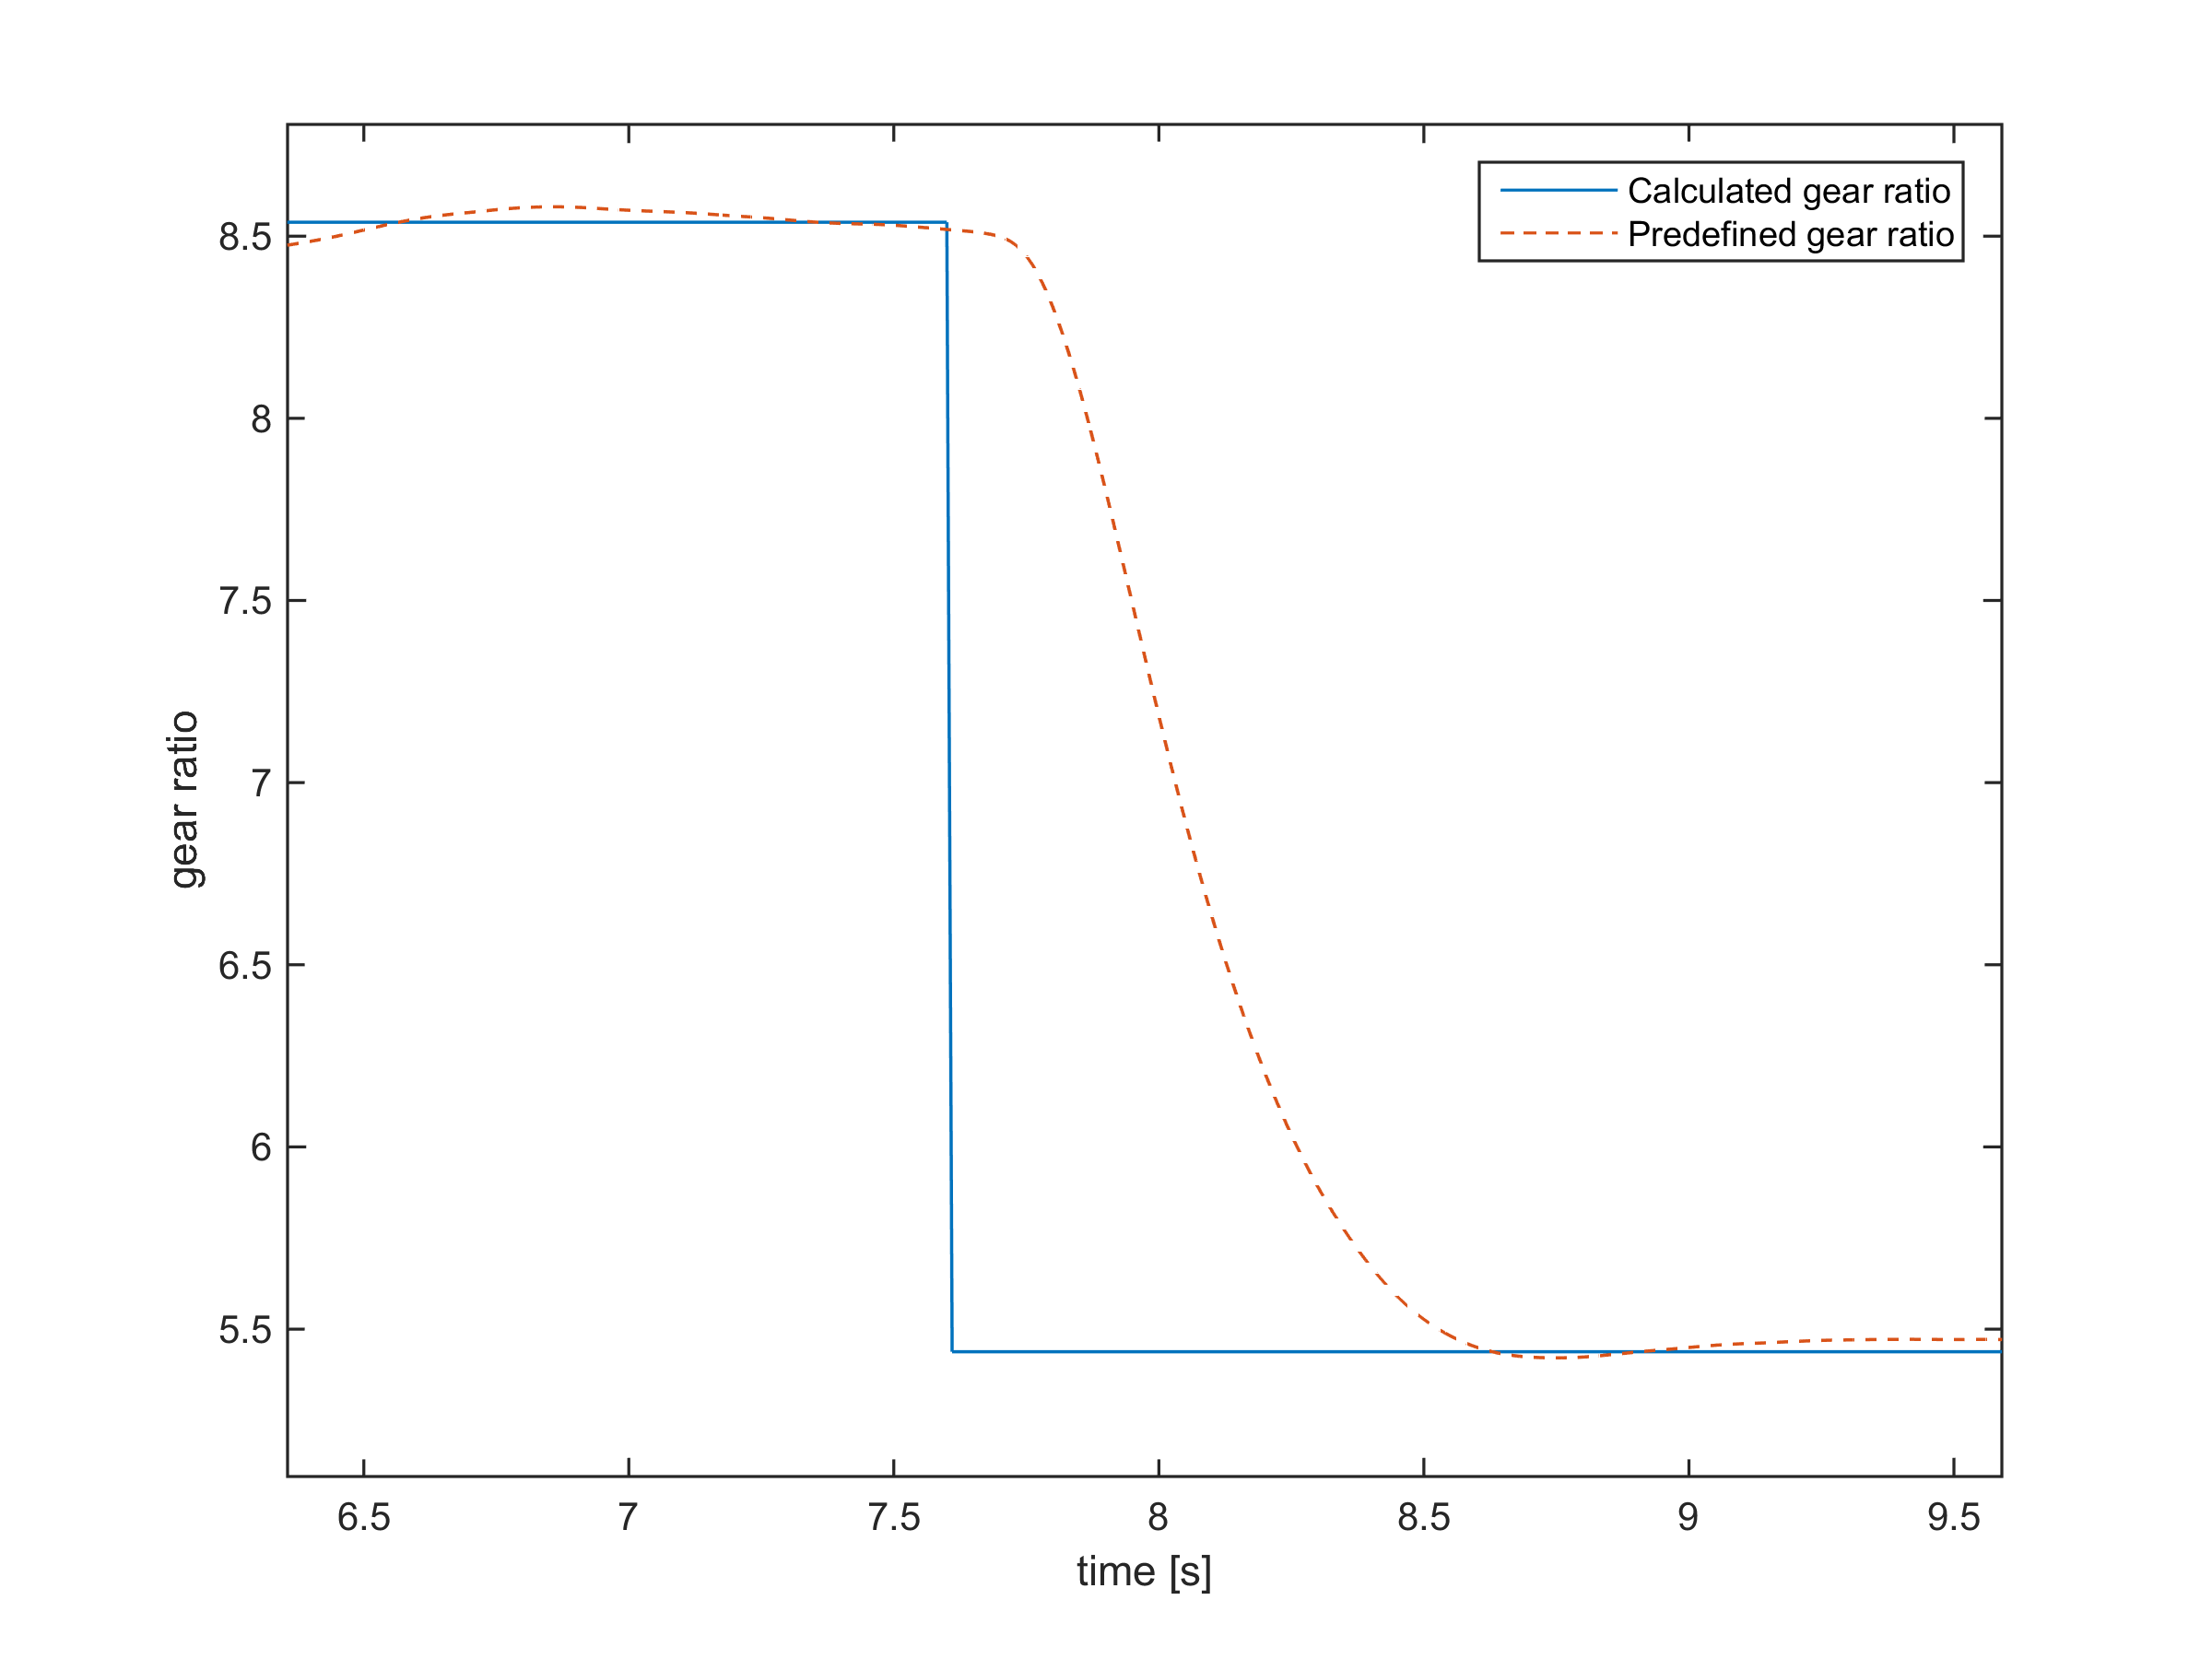
\includegraphics[width=0.8\textwidth]{Pictures/gear_ratio}
	\caption{Calculated and predefined gear ratio in a gear change from 2nd to 3rd gear.}
	\label{gear_ratio}
\end{figure}

\subsubsection{Transfer losses}
There are several factors that affect how much of the engine torque that actually becomes available on the drive shafts. There are several losses in a drive line. Friction and rotating masses within the drive line are the main contributors. Some torque are also lost accelerating the mass of the wheel itself.
\begin{equation}
T_{driveshaft} = T_{driveshaftwithoutlosses}\cdot\eta_{friction}\cdot\eta_{rotating mass} - T_{wheelacceleration}
\end{equation}
$ \eta_{friction} $ is just a scalar factor. The frictional losses are very dependent on the design of the drive line. This means that the losses will differ between vehicles and that this factor needs to be calculated for each specific car model. Since this factor is easy to change it will also include other losses in the drive line such as acceleration of the drive shafts. \todo{can we say this?}

$ \eta_{rotating mass} $ is modeled as:
\begin{equation}
\eta_{rotating mass} = \frac{1}{1 + factor(0.0025?)\cdot gearratio^2}
\end{equation}\\
\todo{choose factor}
The efficiency gets worse as the gear ratio gets higher since there will be more rotating mass in low gears. \todo{is this true?} Just as the frictional losses this loss is also dependent on the design of the drive line. Thus the factor multiplied with the gear ratio needs to be decided for each specific car model.

To calculate $ T_{wheelacceleration} $ requires some more steps. Each wheel connected to a driven shaft has its own moment of inertia which will be accelerated if enough torque is applied. The amount of torque needed to accelerate the wheel depends on its moment of inertia and the angular acceleration:
\begin{equation}
	T = a \cdot I
\end{equation}
The moment of inertia is the wheels radii squared and integrated over the mass. 
\begin{equation}
	I = \int r^2 \cdot dm
\end{equation}
Assuming that a wheel has the shape of a solid cylinder with equal amount of density throughout, the moment of inertia for a wheel can instead be described as:
\begin{equation}
	I = \dfrac{r^2 \cdot m}{2} 
\end{equation}
In the same manner, this applies for the actual drive shafts as well but as was said earlier this loss is included in the scalar factor describing the frictional losses. \todo{again, can we say this?}

The angular acceleration is calculated in the same manner as in Section \ref{longaccest} but now for the front left and right wheel separately.


\subsubsection{Complications}
\todo{this part needs more work}
The main issue with this method is the overall uncertainty of it. For example, the engine torque obtained from the CAN bus isn't measured with a torque sensor on the crankshaft but rather is a calculated value from the engine control unit. The engine control unit calculates the torque with the help several engine parameters and even if it's close most of the times there are moments when it isn't quite right. When doing a sudden acceleration that's aggressive enough to make the vehicle shift down some gears, a so called kickdown, the torque reading will be faulty. 

This method won't work during shifting because the link between the engine shaft and the drive shafts will be lost or affected while the clutch and transmission are working to shift gear. To avoid this trouble the vehicle force estimation simply needs to paused as soon as the start of a gear shift is detected.

\subsubsection{Verification}
Since the reliability of the method is uncertain is needs to be verified in some way. This was done with test data from a driving session where the vehicle was equipped with torque sensors mounted on the drive shafts. By comparing the results from the calculated torque values to the measured values the functionality of the method can be verified. Further on some basic tuning of the efficiency coefficients can be made. In Figure \ref{torque_ver} the verification can be seen.

\begin{figure}[h]
	\centering
	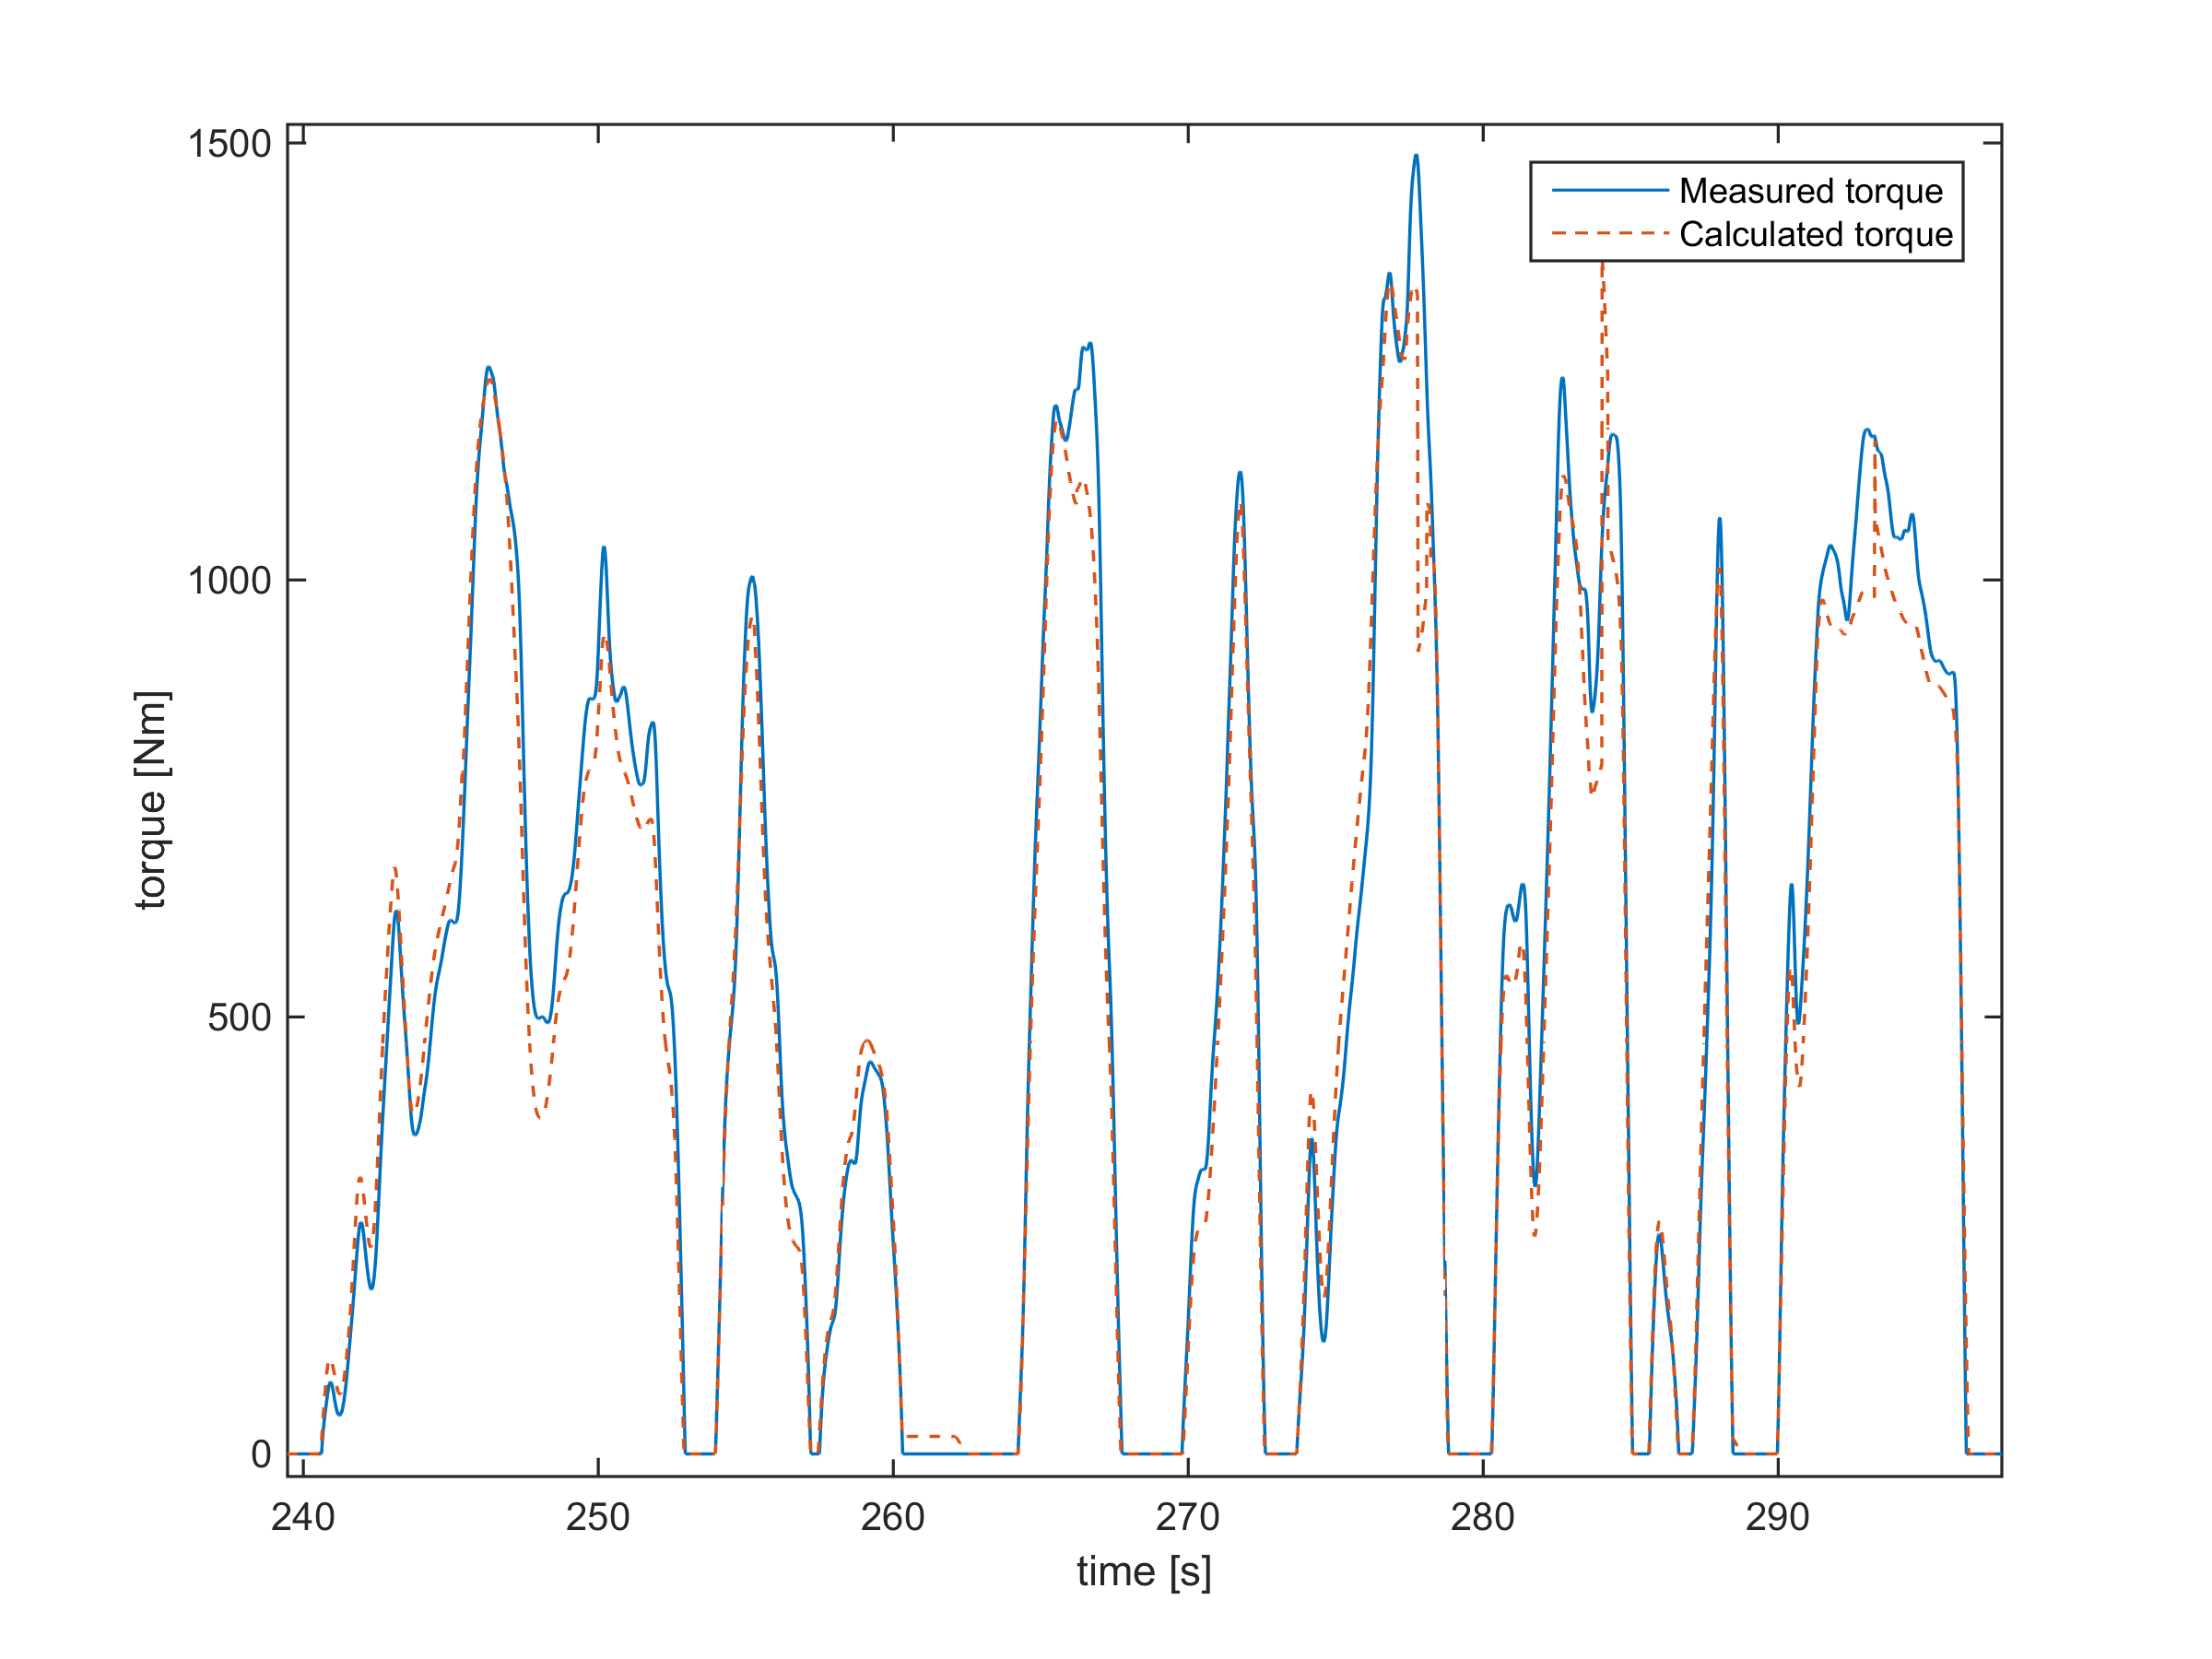
\includegraphics[width=1\textwidth]{Pictures/torque_ver}
	\caption{Measured and calculated torque on the left drive shaft from a vehicle equipped with torque sensors on the drive shafts.}
	\label{torque_ver}
\end{figure}

\subsection{Choosing vehicle model}
Two different models for estimating the vehicle force have been presented. One is based on calculating the force using Newtons second law. This model can be divided into two sub models since the vehicle acceleration can be calculated by derivation of the undriven wheel speed or measured with an accelerometer. The other model uses the engine torque to calculate the vehicle force. Thus, the vehicle force can be acquired in three different ways and it's of course desired to use the most accurate model. When driving in a straight line on a flat road these three models will result in almost the same force, as can be seen in Figure \ref{vehicle_model_comp_olikaacc}. The engine torque model will drop below the other models while shifting gear since the engine is disconnected from the wheels while doing so. This is something that has to be considered, more on this in Section \ref{sec:gearchange}.

\begin{figure}[h]
	\centering
	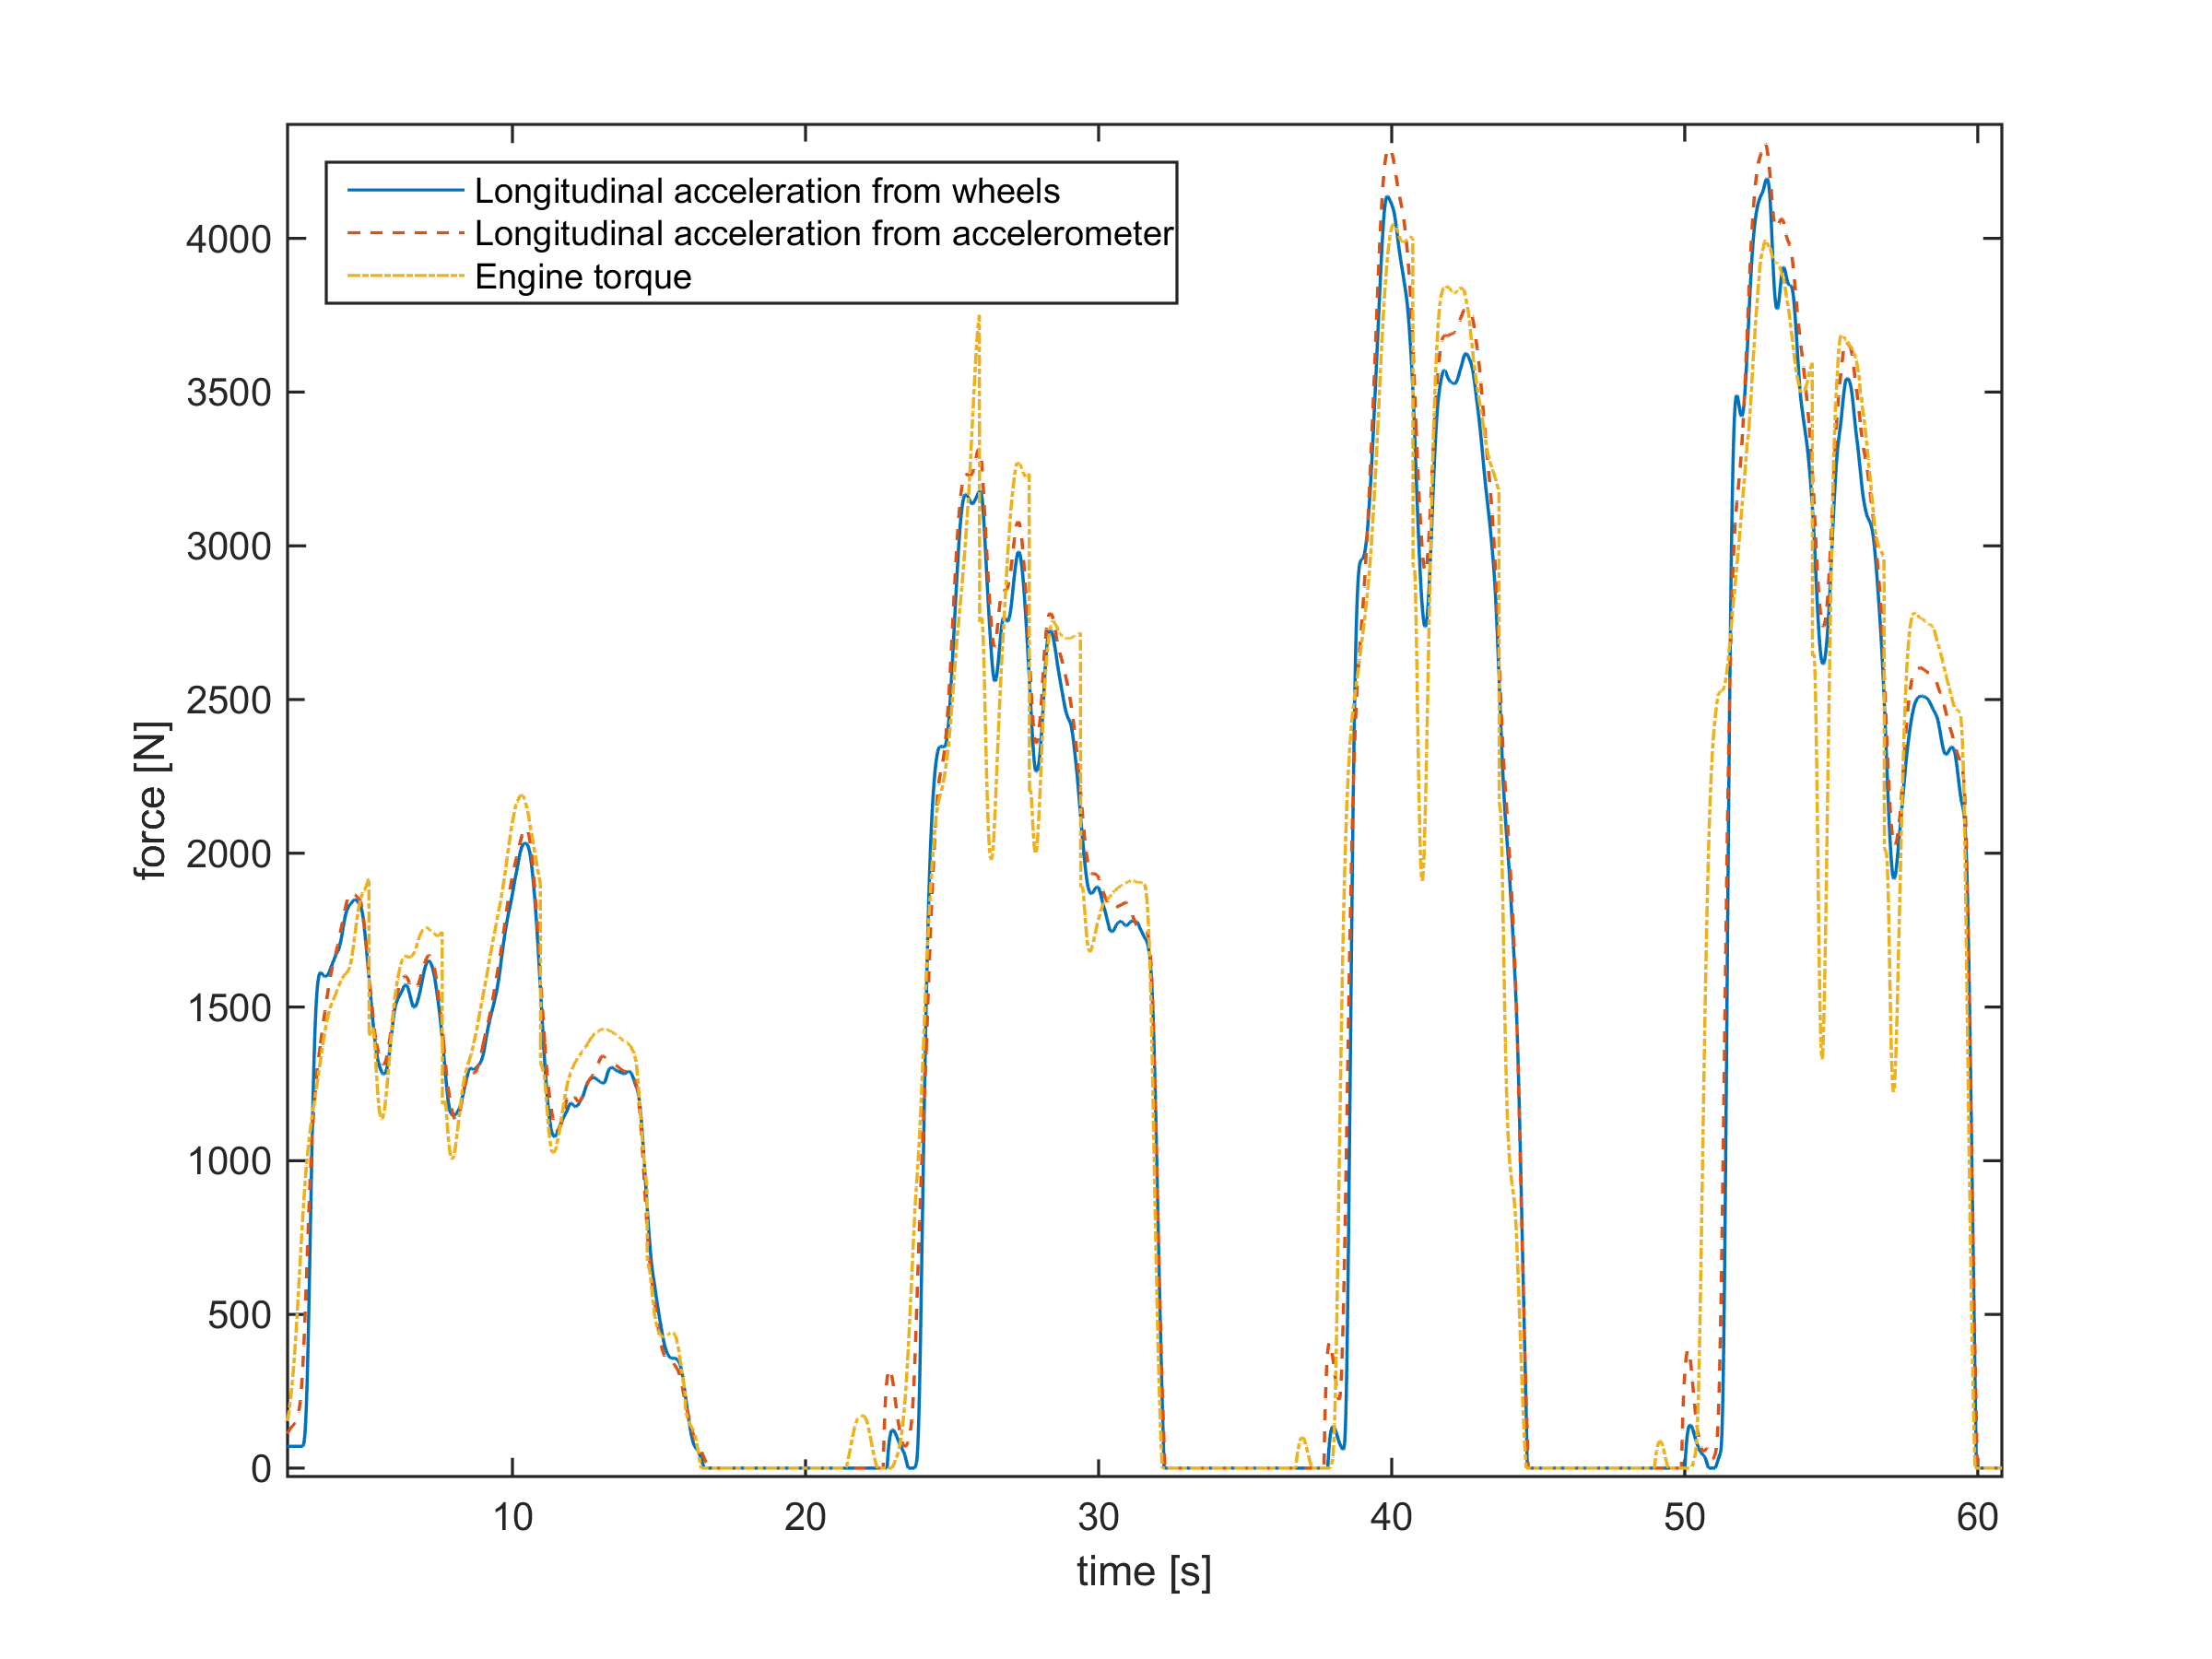
\includegraphics[width=1\textwidth]{Pictures/vehicle_model_comp_olikaacc}
	\caption{The vehicle force for the three different models while driving in a straight line on a flat road.}
	\label{vehicle_model_comp_olikaacc}
\end{figure}

The models will differ more when cornering, as can be seen in Figure \ref{vehicle_model_comp_race}. Neither the acceleration calculated from the undriven wheel speed or the measured acceleration from the accelerometer will be true while cornering. This is because both solutions for acquiring the vehicle acceleration is for longitudinal acceleration only. The undriven wheels is in this case the rear wheels and since these can't turn only the longitudinal acceleration is represented. The same goes for the accelerometer, only the longitudinal part of the acceleration is measured. The actual acceleration of the vehicle while cornering is a combination of longitudinal and lateral acceleration. The result of all this is that the force from the acceleration based vehicle models gets to low when cornering. 

\begin{figure}[h]
	\centering
	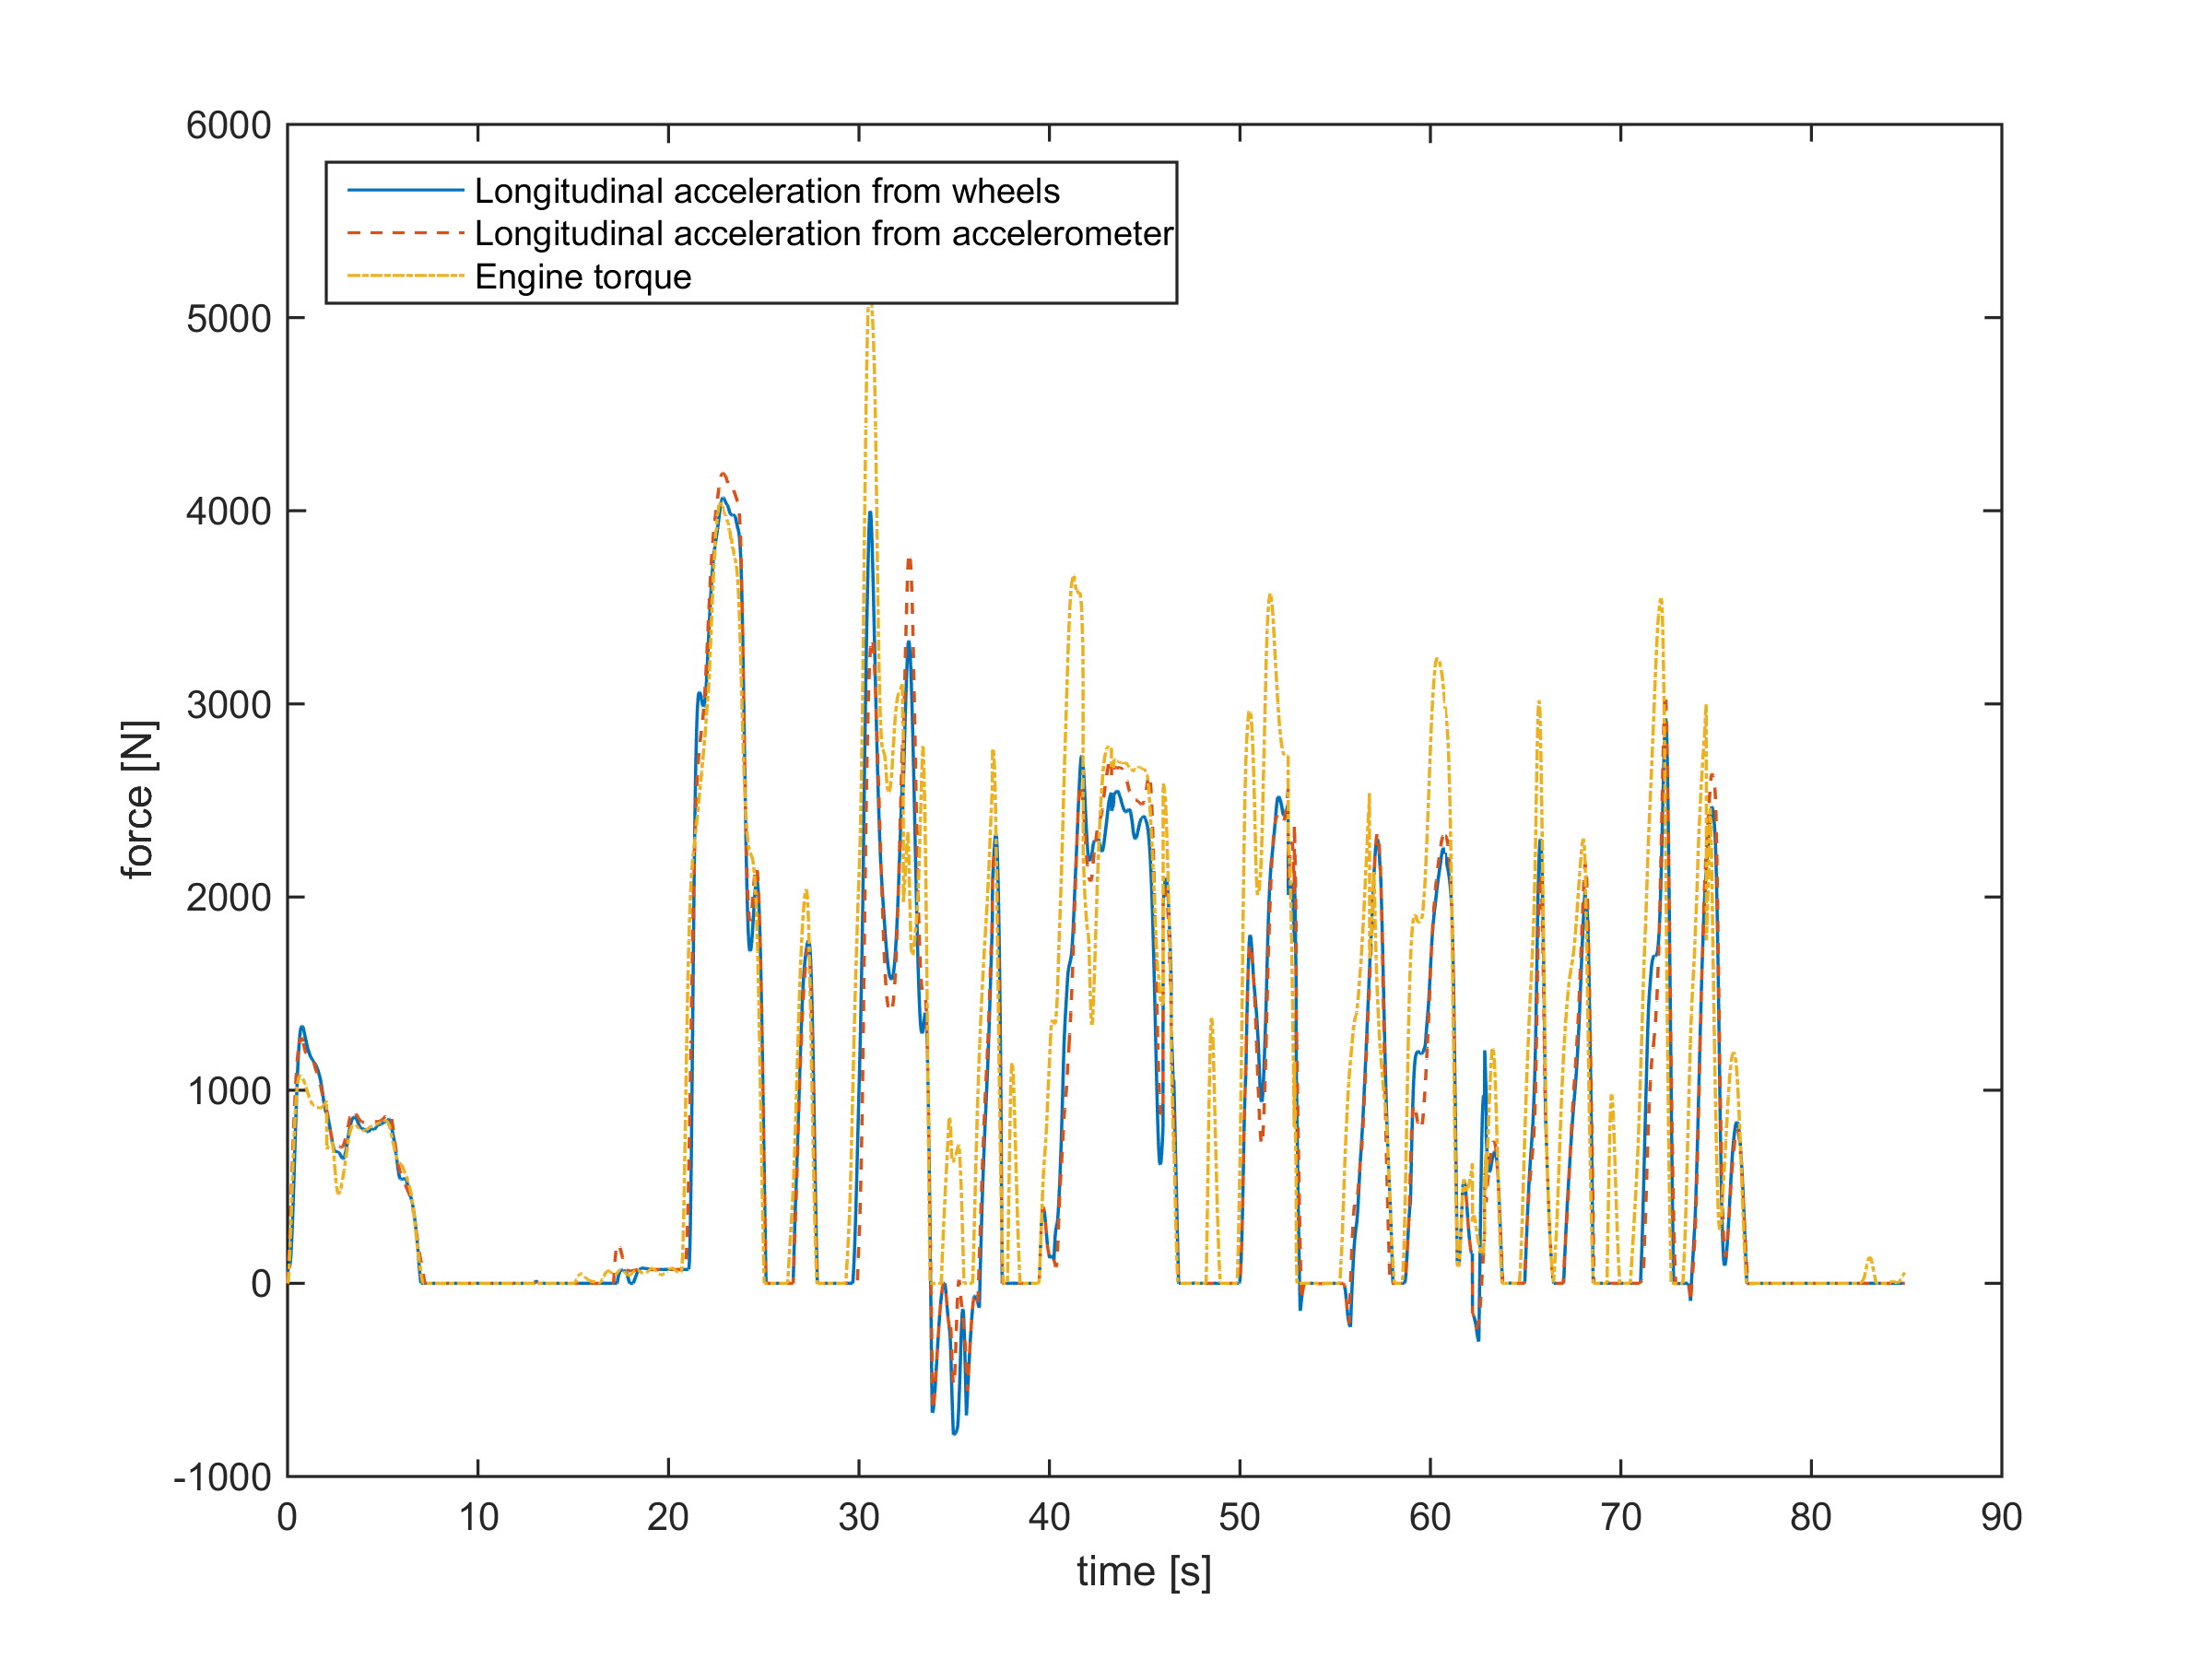
\includegraphics[width=1\textwidth]{Pictures/vehicle_model_comp_race}
	\caption{The vehicle force for the three different models while driving along a track with several corners.}
	\label{vehicle_model_comp_race}
\end{figure}

A solution to this could be to measure both the longitudinal and lateral accelerations with accelerometers and calculate the total acceleration of the vehicle. Unfortunately it's not that easy. When using both longitudinal and lateral acceleration of the vehicle the tire models must be able to account for both longitudinal and lateral force which is hard to model. More on this in Section \ref{tire_forces}.

It get's even worse when driving on a road that's hilly, as can be seen in Figure \ref{vehicle_model_comp_mm2}. While driving uphill or downhill the longitudinal acceleration from both the calculations and the accelerator measurements will be wrong. \todo{still no sure of this} The drive session shown is uphill, hence the force will be to low since the force needed to counter the force of gravity isn't considered. When cornering both acceleration based models where almost equally faulty at all time. When driving in a hill there's a difference between them. This is because the model based on undriven wheel acceleration won't consider the force of gravity at all. The model based on the accelerometer will consider it to some extent since the accelerometer will incline with the car, although, it won't be right.

The acceleration based vehicle models have been discussed a lot so far. The model based on engine torque hasn't been mentioned much at all and it has even been implied that this one is correct when the acceleration based models are falling behind. This is because it really is a good model that fills it purpose. It's not affected by hills and it's not as severely affected by cornering as the acceleration based models are. The force will always be applied in the longitudinal direction of the tire, hence it works good to match this with a longitudinal tire model. The main problem is the fact that the slip calculation will be a bit off while cornering since lateral velocity isn't considered but this is solved later on in Section \ref{sec:latacccomp}. 

All in all, the obvious choice is the engine torque based vehicle model.

\begin{figure}[h]
	\centering
	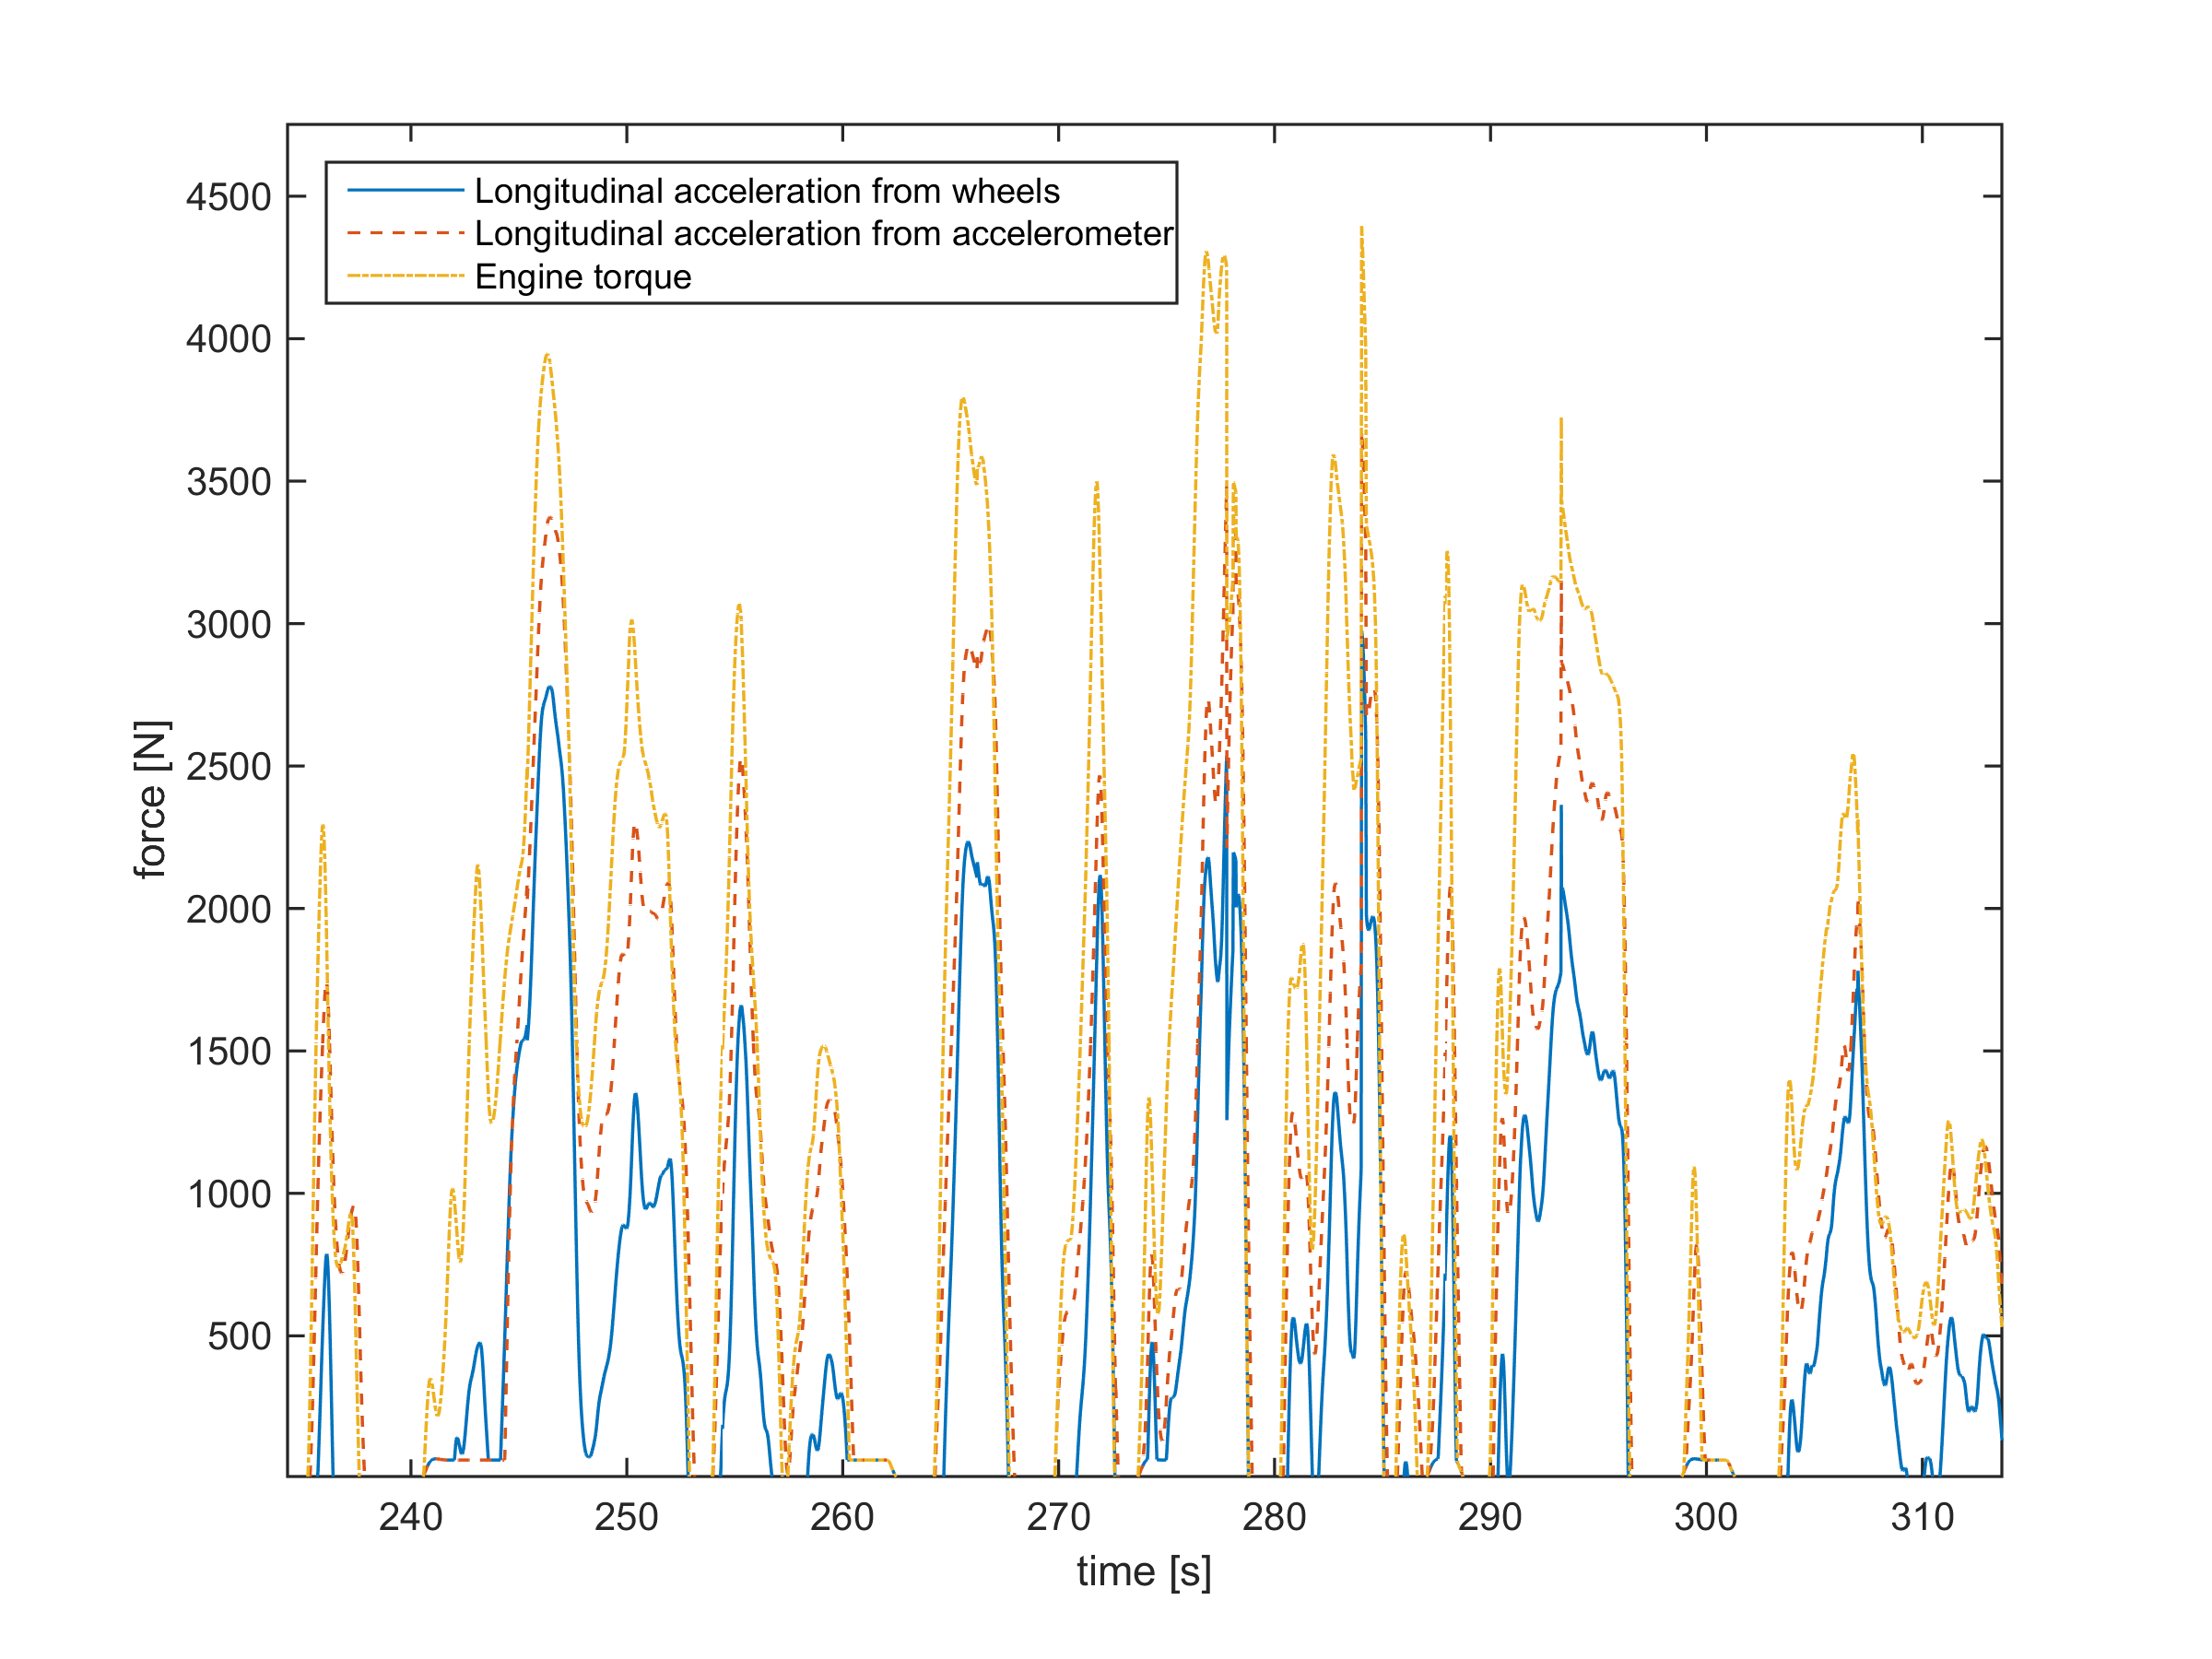
\includegraphics[width=1\textwidth]{Pictures/vehicle_model_comp_mm2}
	\caption{The vehicle force for the three different models while driving along a track with several corners and hills.}
	\label{vehicle_model_comp_mm2}
\end{figure}

\section{Tire forces}
\label{tire_forces}
The characteristic of a tire is very complex, which makes the actual force generated to the vehicle difficult to obtain. As was shown in the theory, Section \ref{sec:tire_models}, there are several tire models that can be used, everyone of them with different properties.

A tire can generate both longitudinal and lateral force. It's quite easy to create a tire model that considers both these forces, the hard part is to acquire all the input parameters to the model in real time while driving. The parameters to model the lateral force are especially hard to obtain. These parameters are the slip angle and the lateral tire stiffness. Since these are so hard to calculate only the longitudinal part of a force model is used. The main dynamic parameters of a longitudinal tire force model (except Magic formula) includes the slip ratio, normal force, and the tire/road friction coefficient. A fourth, less dynamic parameter is the longitudinal tire stiffness. 
\begin{equation}
F_{tire, longitudinal} = f(\kappa, Fz, \mu, C_{x})
\end{equation}
The slip ratio is calculated from the wheels difference in angular and forward velocity as seen in Equation $ \ref{eq:longslip} $, the normal force from the weight of the vehicle and the changing weight distribution derived in  Section \ref{normal_force}, and the tire stiffness as explained in Section \ref{sec:tire_stiffness}. Thereafter, the only dynamic parameter of the tire force equation becomes the friction coefficient. By choosing the correct $ \mu $, the force from the tire model will equal the force from the vehicle model. This calculation is done in a feedback manner, meaning that the tire force depends on the friction coefficient derived in the previous iteration.

\subsection{Choosing a tire model}
Four models where described in the theory part. Brush model, Dugoff model, Magic formula and a tire model created by Ola Nockhammar at Borg Warner AB, further on called Ola's model.

The magic formula was ruled out almost immediately since it's a too complicated model to be adaptive enough. It's great for simulating a specific tire in a lab for example but using it in a real time car environment won't work. It's just too many parameters to estimate when switching from summer to winter tires for example. \todo{hmm?}

The other three models are more simple with fewer input parameters and above all it's parameters that are more easily available, like slip ratio and normal force. The Brush model and the Dugoff model are even too simple. The only available parameter to change the characteristics of the slip/force curve is the longitudinal tire stiffness. Ola's model on the other hand contains two degrees of freedom by introducing a second parameter to affect the inclination of the slip/force curve. Hence, it's easier to model a tire correctly with this model. Another positive aspect is the fact that the model is made for longitudinal force estimation only. Thus, it doesn't need to be modified for longitudinal use only like the Brush and Dugoff models. \todo{is this true?}

All in all, Ola's model was the obvious choice for this work.

\subsection{Tire model parameters for Ola's tire model}
In this section the four model parameters that affects Ola's tire model will be explained in more detail.

\subsubsection{Tire stiffness}
The tire stiffness is obtained by deriving the tire force generated per slip for values around zero, i.e. the gradient of the slip/force curve at zero slip. The slip force curve for two different tire stiffnesses can be seen in Figure \ref{different_cx}. The interpretation from this figure is that a tires stiffness is an essential parameter to have in order to model the tire force correctly. 

\begin{figure}[h]
	\centering
	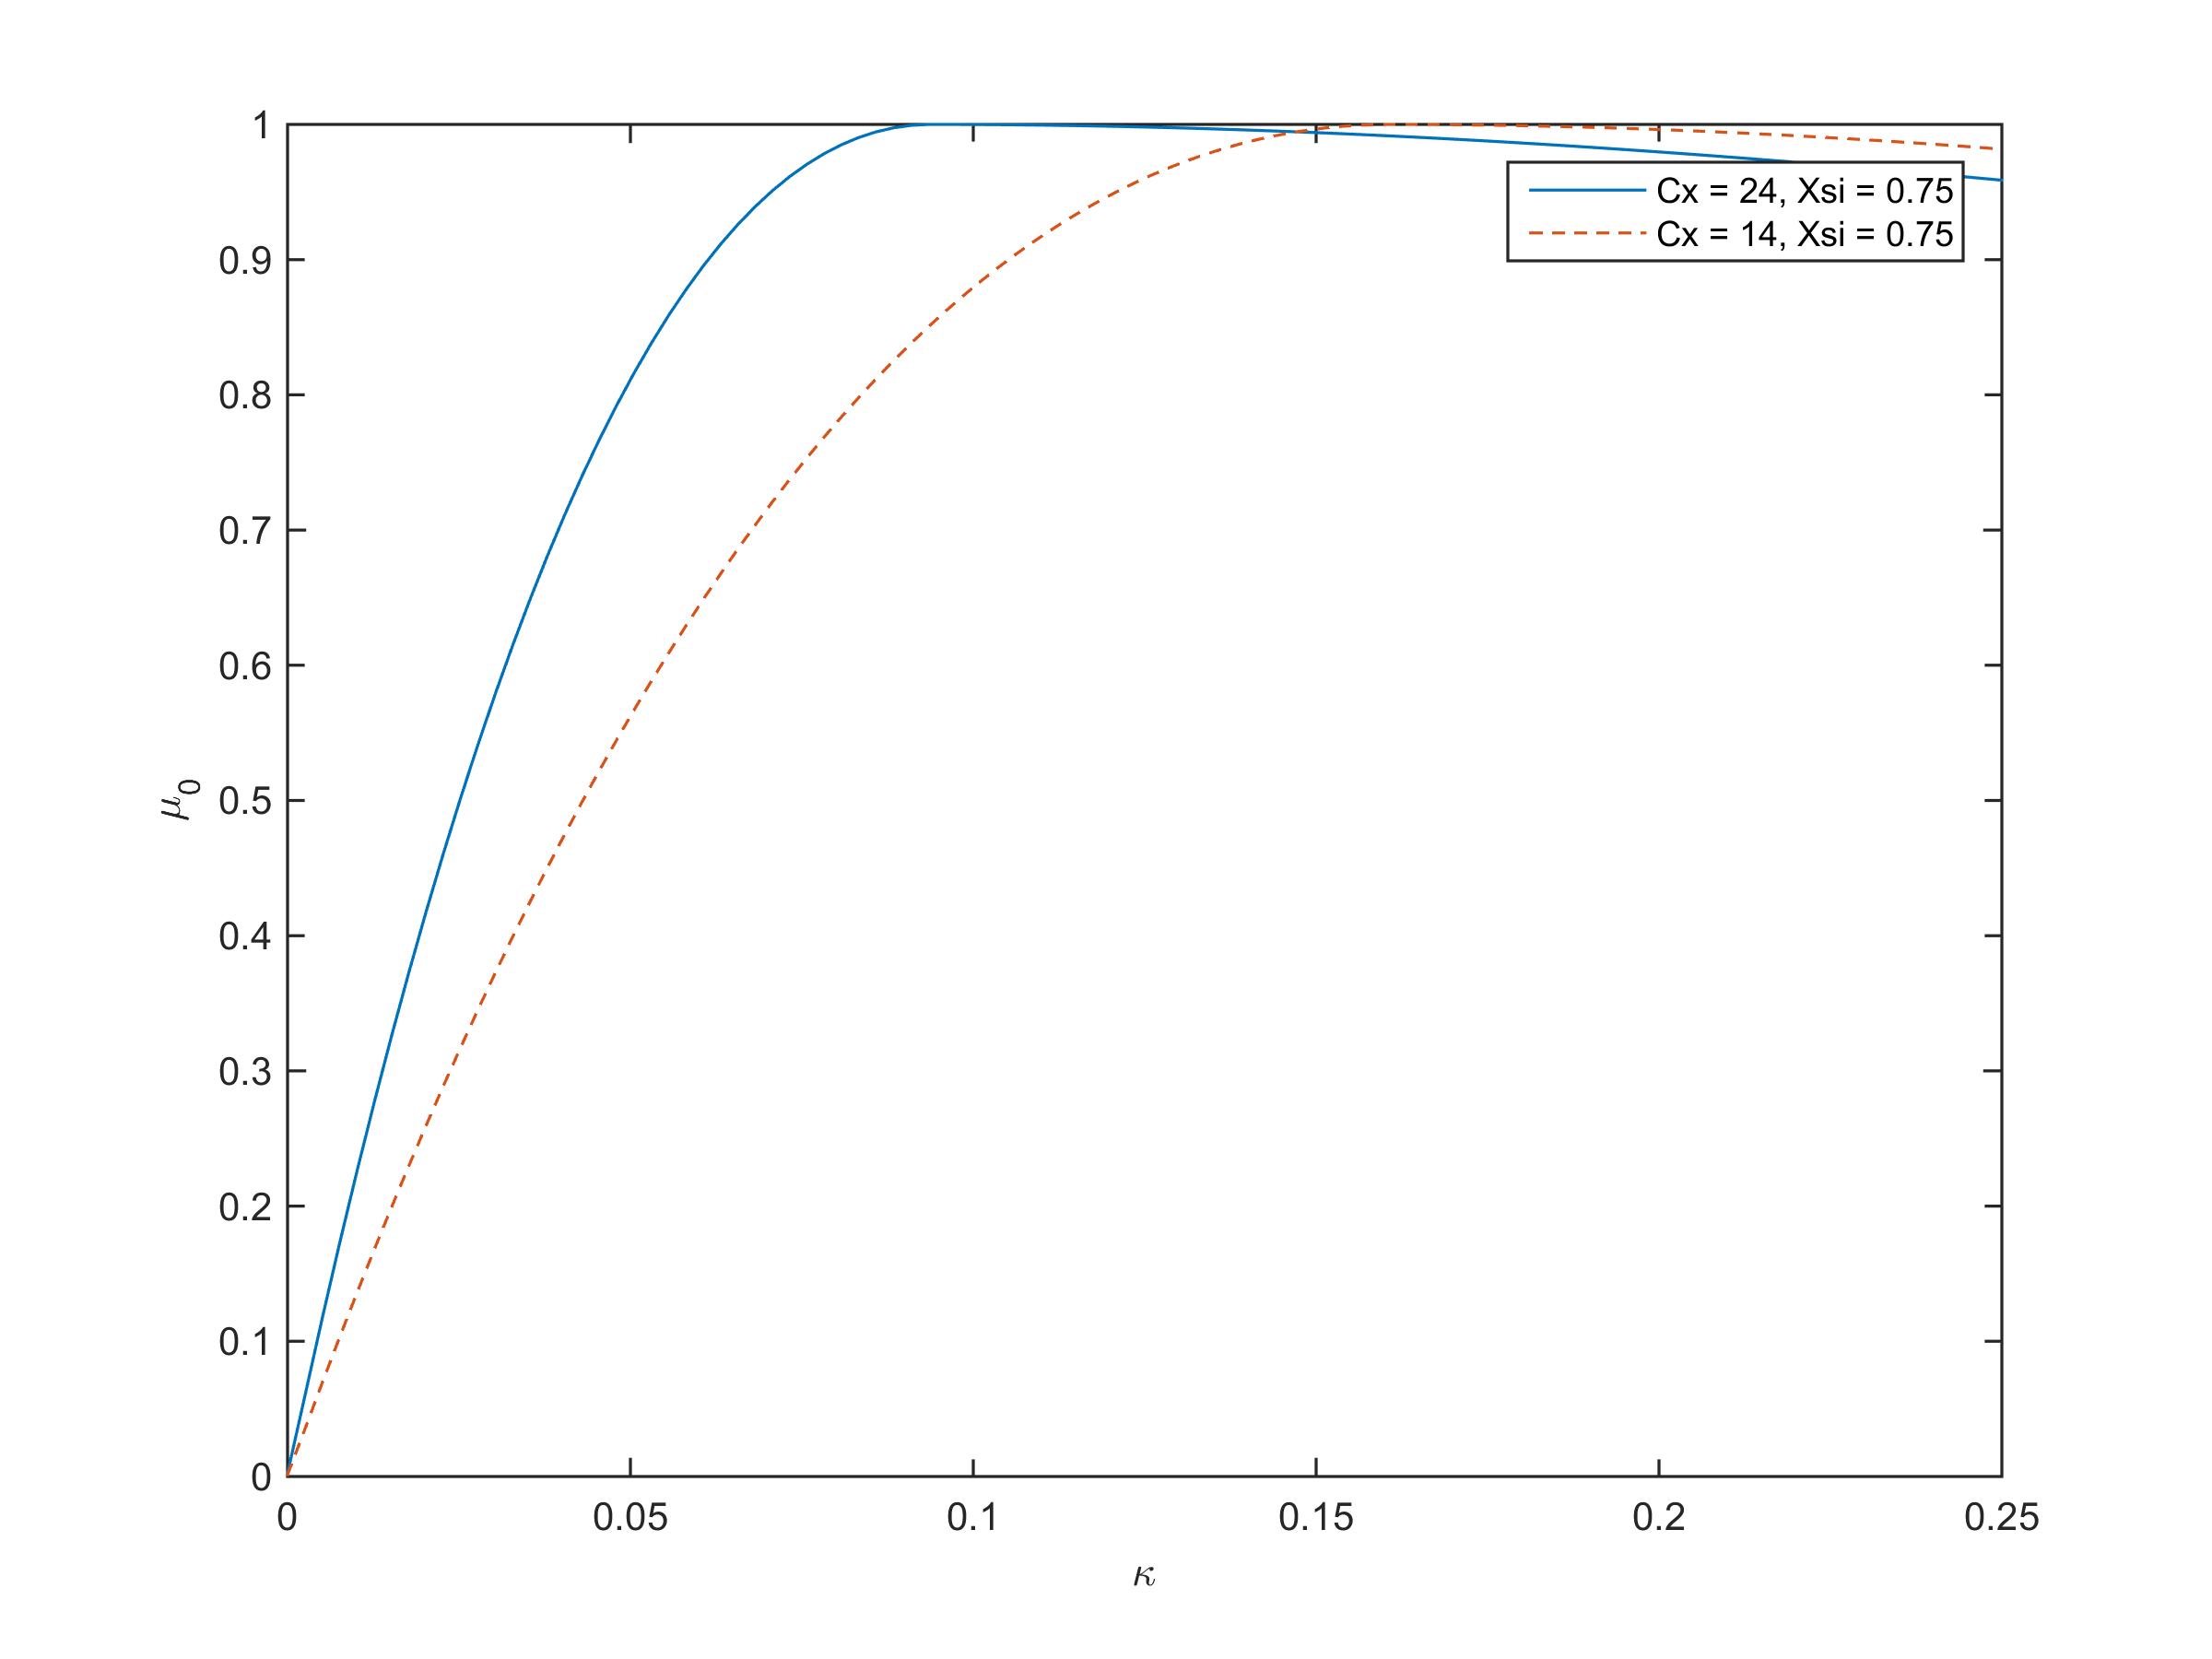
\includegraphics[width=0.8\textwidth]{Pictures/slipkraft_olika_cx}
	\caption {Normalized tire model force per slip ratio for different tire stiffnesses. $ \mu = 1.0 $.}
	\label{different_cx}
\end{figure}

Unfortunately, a tires characteristics is further complex, and cannot be explained by the tire stiffness as a parameter alone. Two different tires can have the same tire stiffness, but differing characteristics at larger slip ratio values. An example of this can be seen in Figure \ref{different_xsi}. Generally, tires with lower tire stiffness value have higher $ \xi $, hence resulting in even lower forces for higher slip values.\todo{is this true?} Once again this is a good reason to use Ola's tire model since $ \xi $ can be modified in this model.

\begin{figure}[h]
	\centering
	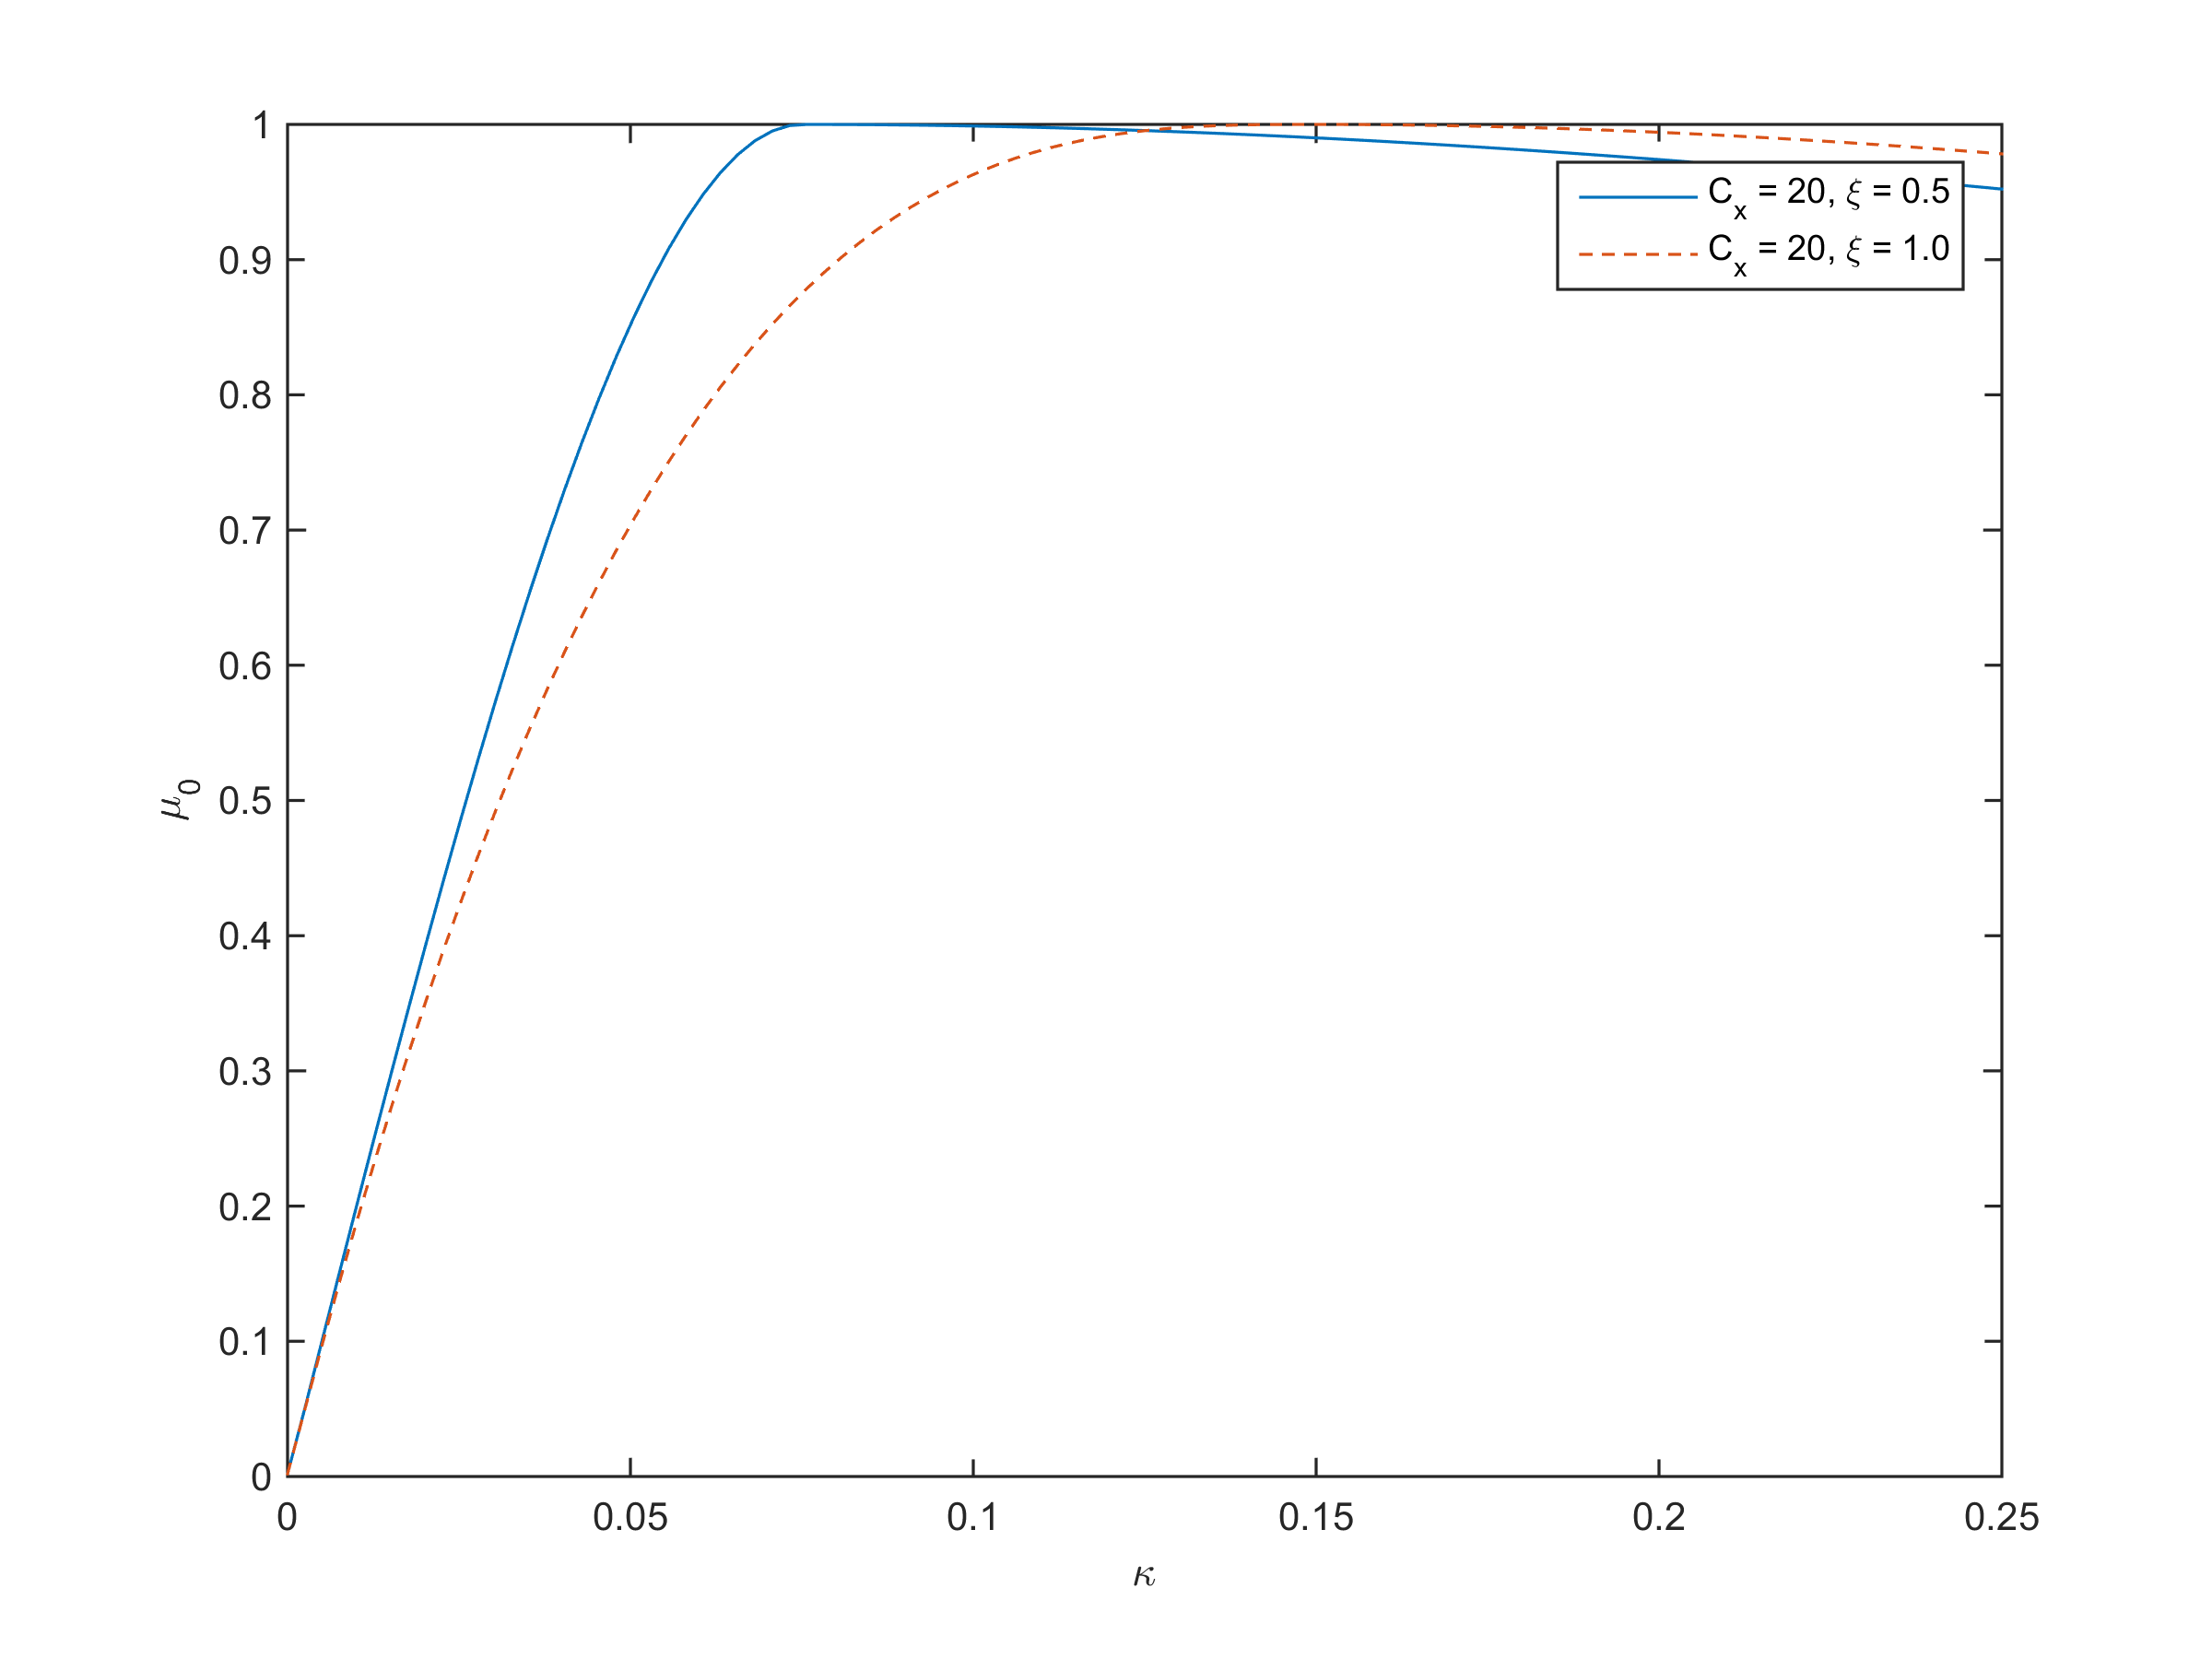
\includegraphics[width=0.8\textwidth]{Pictures/slipkraft_olika_xsi}
	\caption {Normalized tire model force per slip ratio for different tire characteristics for higher slip ratios.
		$ \mu = 1.0 $.}
	\label{different_xsi}
\end{figure}

The tire stiffness for a certain tire should theoretically be the same for different road surfaces. Nevertheless, testing has shown that the actual inclination of the slip/force curve for small slips can differ for different road surfaces. The tire stiffness therefore has to be compensated accordingly depending on the roads friction coefficient. \todo{this needs to be exaplained in more detail}

\subsubsection{Slip ratio}
As seen most slip/force figures, the maximum force will be generated at a specific slip and will thereafter decrease with an increasing slip ratio. If the tire model doesn't capture this force peak at the correct slip ratio value, it will become very difficult to match the tire model force with the calculated vehicle force. The slip ratio value during a real driving sequence is usually rather small (maximum force is generally obtained at a slip ratio $ \geq 12 \% $), which means that a small variances in the slip ratio calculations will have a large impact on the resulting force.

In order to calculate the slip ratios of the two front wheels, the four wheel speeds are gathered from the vehicles CAN bus. These signals generally include quite a lot of measurement and/or process noisy which thereafter leads to a noisy slip ratio calculation, as can be seen in the first row of Figure \ref{wheel_speed_and_slip}. In order to overcome this noise and capture the actual value, the signals are run through a low pass filter. The wheel speeds will, even after filtering, have an oscillating attribute. When theses oscillations from the front and its respective rear wheel are not synchronized and with different magnitude, the calculated slip ratio will have rather large variation compared to its real value. This can be seen in the second row of Figure \ref{wheel_speed_and_slip}, where the wheel speeds are run trough a relatively slow low pass filter, i.e. a low pass filter with a high cutoff frequency. Most of the measure and/or process noise is removed, but due to the characteristics of the wheel speed sensor and its design, the signal will still oscillate with a frequency that is proportional to its angular velocity. To minimize the error from the oscillations, the wheel speeds are filtered with a lower cutoff frequency, which can be seen in the third row of Figure \ref{wheel_speed_and_slip}. 
\begin{figure}[h]
	\centering
	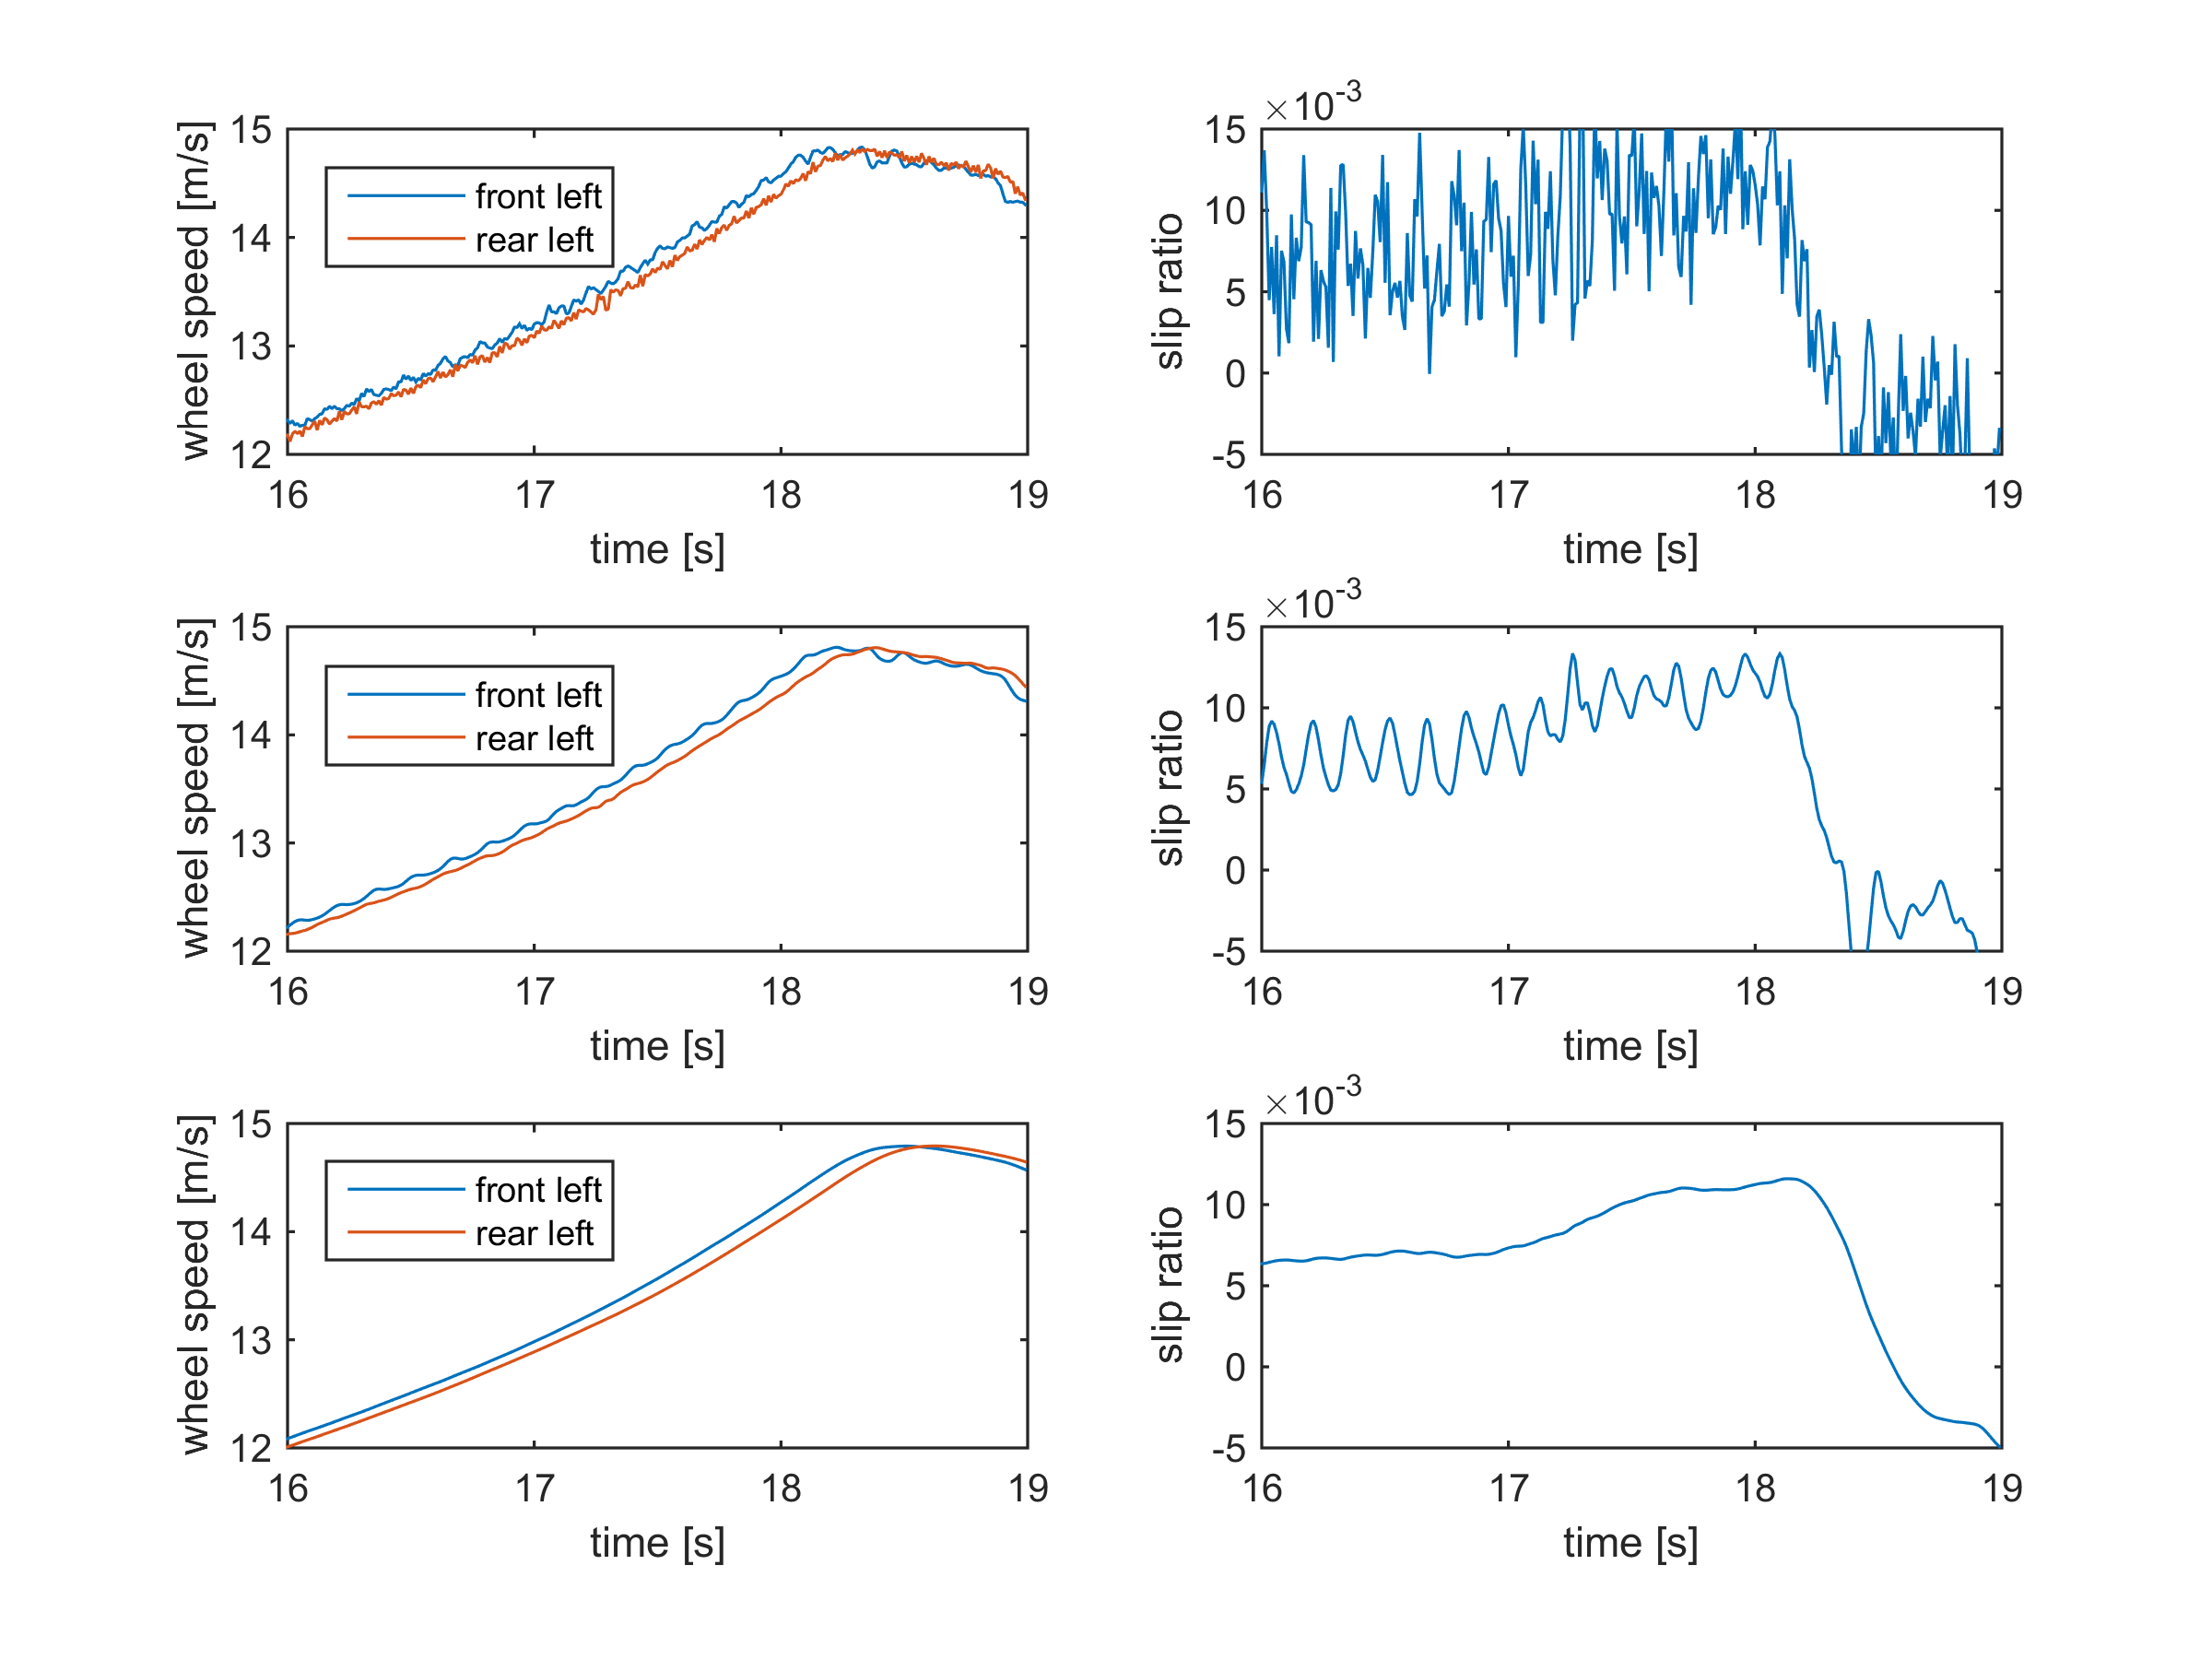
\includegraphics[width=1.0\textwidth]{Pictures/wheel_speed_and_slip}
	\caption {Wheel speeds and slips for different filters.}
	\label{wheel_speed_and_slip}
\end{figure}
Another concrete problem that arises when calculating the slip ratio, is that the radius for each wheel on a vehicle can be different, e.g. when the air pressure of a tire drops slightly over time. The wheel speed from the CAN bus will in this case be wrong, leading to a offset in the slip ratio calculations. \todo{explain more}

\todo{Skriva något fint om kraften med slip angle} The force/slip should be smaller when the slip angle is larger. In other words, when we have more lateral force, the longitudinal force will be smaller.

\subsubsection{Normal force}
The amount of longitudinal force (neglecting lateral forces) generated from a tire depends on the normal force acting on the tire. The force generated by a tire is linearly proportional to the normal force on the tire:
\begin{equation}
	F_{x} = F_{z}\mu_{0}
\end{equation}
Where the normalized force $ \mu_{0} $, never can exceed the friction coefficient between the tire and the road:
\begin{equation}
	\mu_{0} \leq \mu
\end{equation}
It is therefore important to know the loaded weight on each tire at every instant. This is done by the dynamic weight distribution calculations explained in Section \ref{normal_force}. These calculations are rather simplified, where the difference in chassis stiffness between front and back is not considered. These chassis stiffnesses are vehicle specific and hard to estimate. 

This means that the maximum longitudinal force obtained by either the vehicle model or the tire force model, can never be larger than the normal force multiplied by the tire/road friction coefficient, which can be helpful to rule out unreasonable values. 

\subsubsection{Friction coefficient}
\label{section_friction coefficient}
The final dynamic parameter that affect the tire force model is the friction coefficient between the tire and the road. The friction coefficient limits the normalized force that can be generated through the tires, which means that the friction coefficient and the normal force, $ F_{z}\mu $, limits the amount of longitudinal force possible to acquire. How different $ \mu $ affects the force/slip curve for Ola's tire model can be seen in Figure \ref{different_mue}. For a certain slip ratio value, different normalized force values will be acquired for the variant friction coefficient. It should also be noted in the figure that the derived force will not differ greatly depending on the friction coefficient at low slip ratio values. It is therefore desired to have a somewhat larger slip ratio value before the estimating the friction coefficient value. In other words, the normalized force should be closer to the frictional limit in order to acquire a more correct friction coefficient. 

\begin{figure}[h]
	\centering
	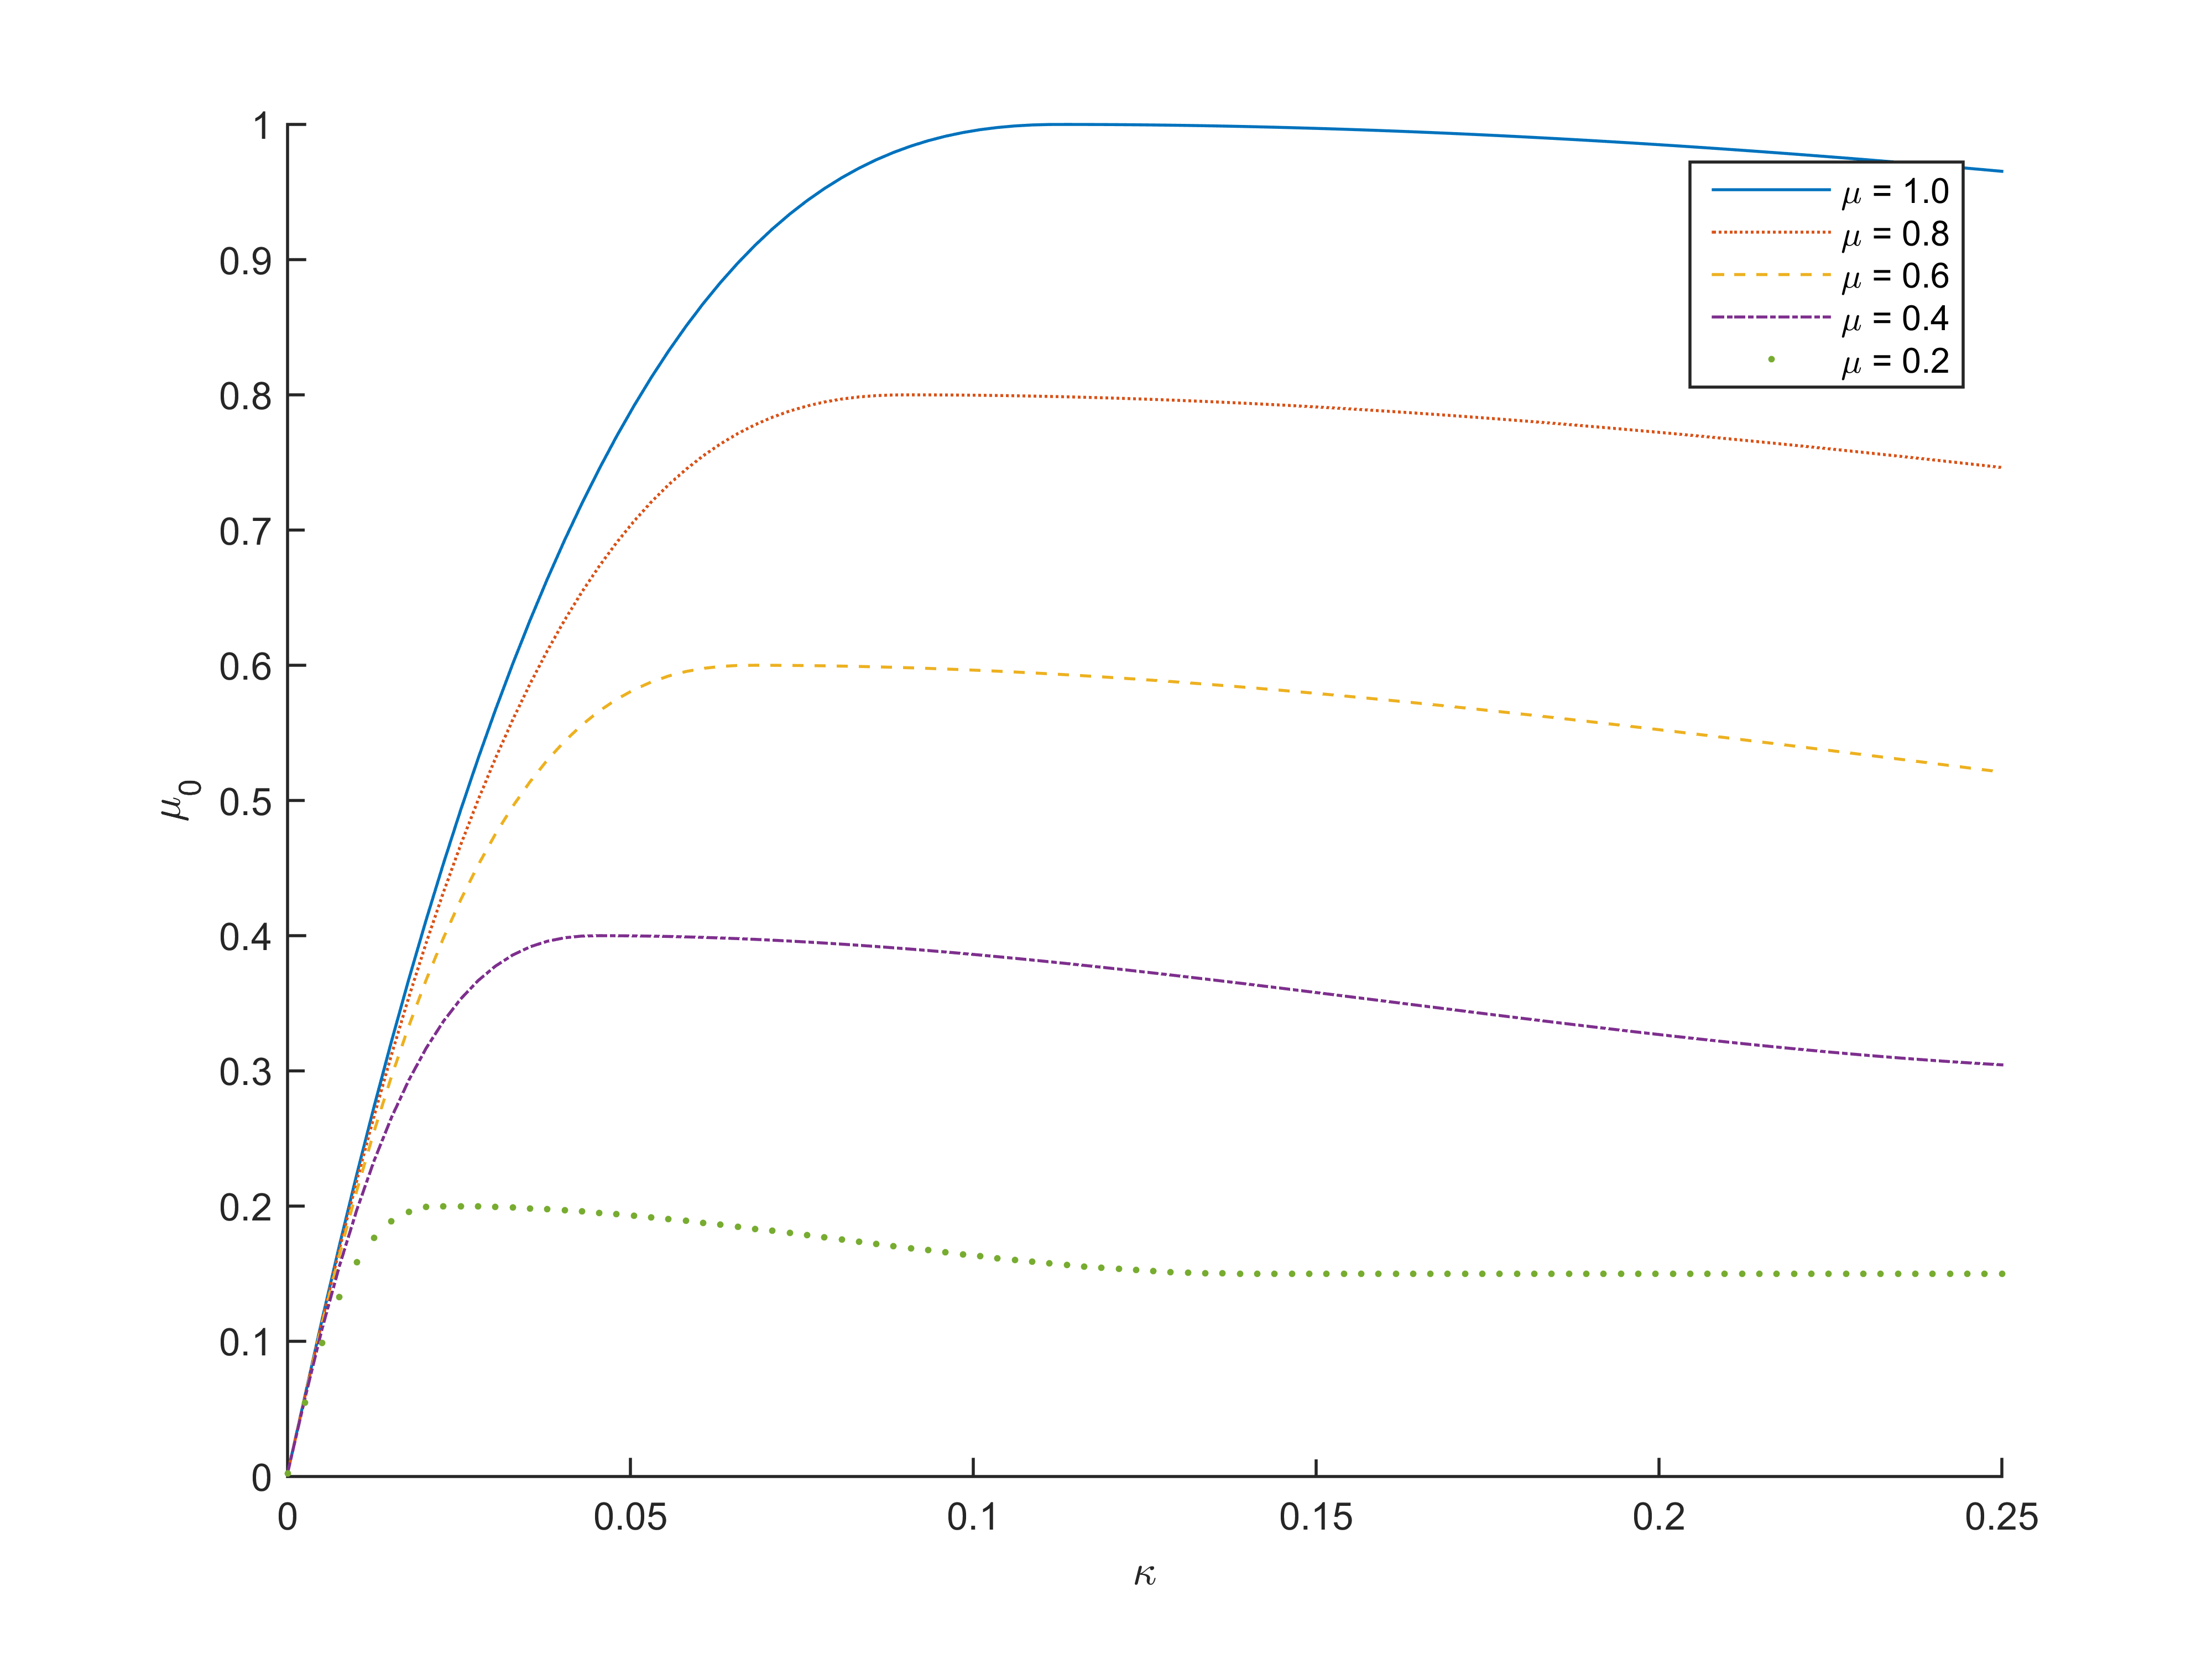
\includegraphics[width=0.8\textwidth]{Pictures/slipkraft_olika_mue}
	\caption {Normalized tire model force per slip ratio for different mue values.}
	\label{different_mue}
\end{figure}

\section{Fitting the tire model}
It is, as seen Section \ref{tire_forces}, very important to know the parameters that affect the force derived from the tire model. Slip ratio and the normal force is derived by using CAN signals from the vehicle and the friction coefficient is the parameter that should be approximated. The tire stiffness on the other hand is harder to approximate with good accuracy. The definition is, as mentioned earlier, the gradient of the slip/force curve around zero slip ratio, which means that the tire stiffness should preferably be approximated at small slip ratio values, where the gradient is relatively constant. The force per slip ratios between $ 0 $ and $ 2 $ can be seen in Figure \ref{slip_kraft_sma_slip}. The figure shows that the variance of the force per slips ratio is rather large around the approximated line at $ C_{x} = 24 $. These tire stiffness variations for different driving scenarios makes it very hard to approximate the tire stiffness in a correct manner.

\begin{figure}[h]
	\centering
	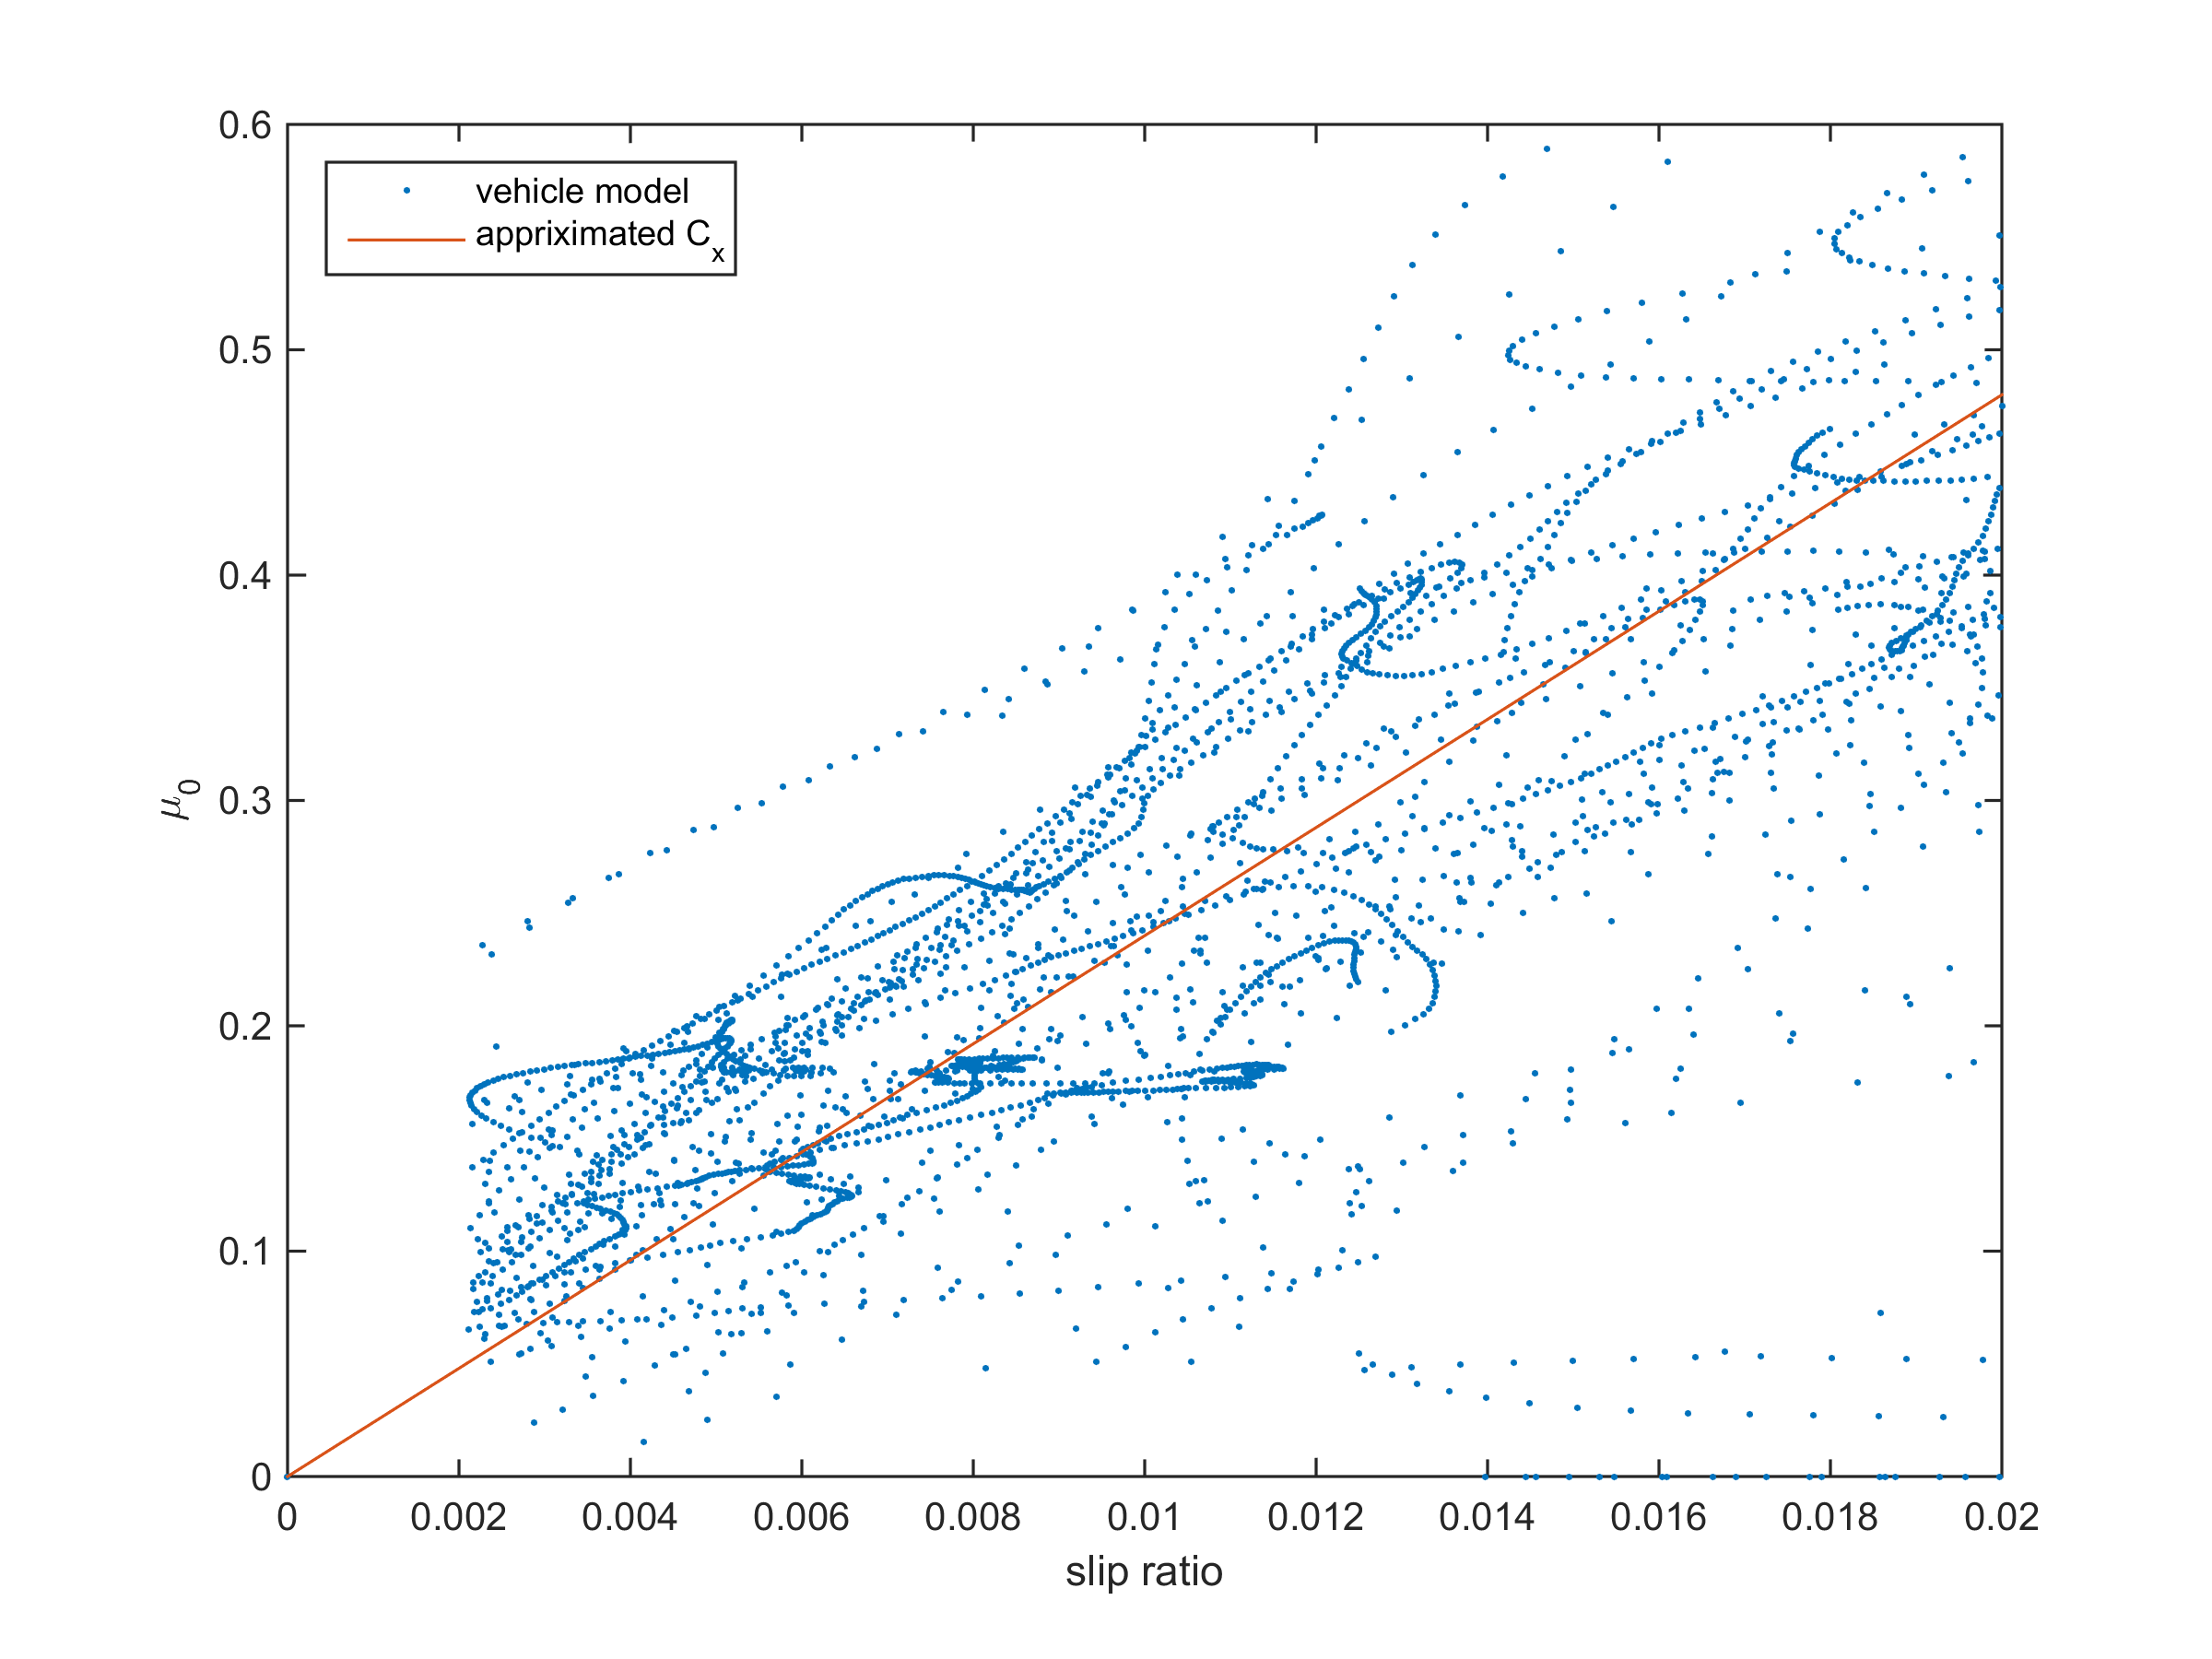
\includegraphics[width=0.8\textwidth]{Pictures/slip_kraft_sma_slip}
	\caption {Force per slip for lower slip ratio values can be used to estimate the tire stiffness.}
	\label{slip_kraft_sma_slip}
\end{figure}

Due to the difficulties to estimate the tire stiffness, experimentations has been made to fit tire model parameters during test driving. The problem with this solution is that static tire model parameters would be chosen for a certain driving sequence instead of having a dynamic solution that works for every kind of tire. 

It was also found during testing that the tire stiffness for the same set of tires changes depending on friction coefficient between the tire and the road. The tire stiffness will therefore be interpolated between two different tested tire stiffness values depending on the friction coefficient.

\subsection{Winter tires}
\label{winter_tire}
Test driving has been done with a set of winter tires on both asphalt and ice/snow. In Figure \ref{slip_kraft_ljungby} the force per slip can be seen during a simple acceleration run on asphalt. It should be noted that only values for when the actual friction estimation is active is used. 

\begin{figure}[h]
	\centering
	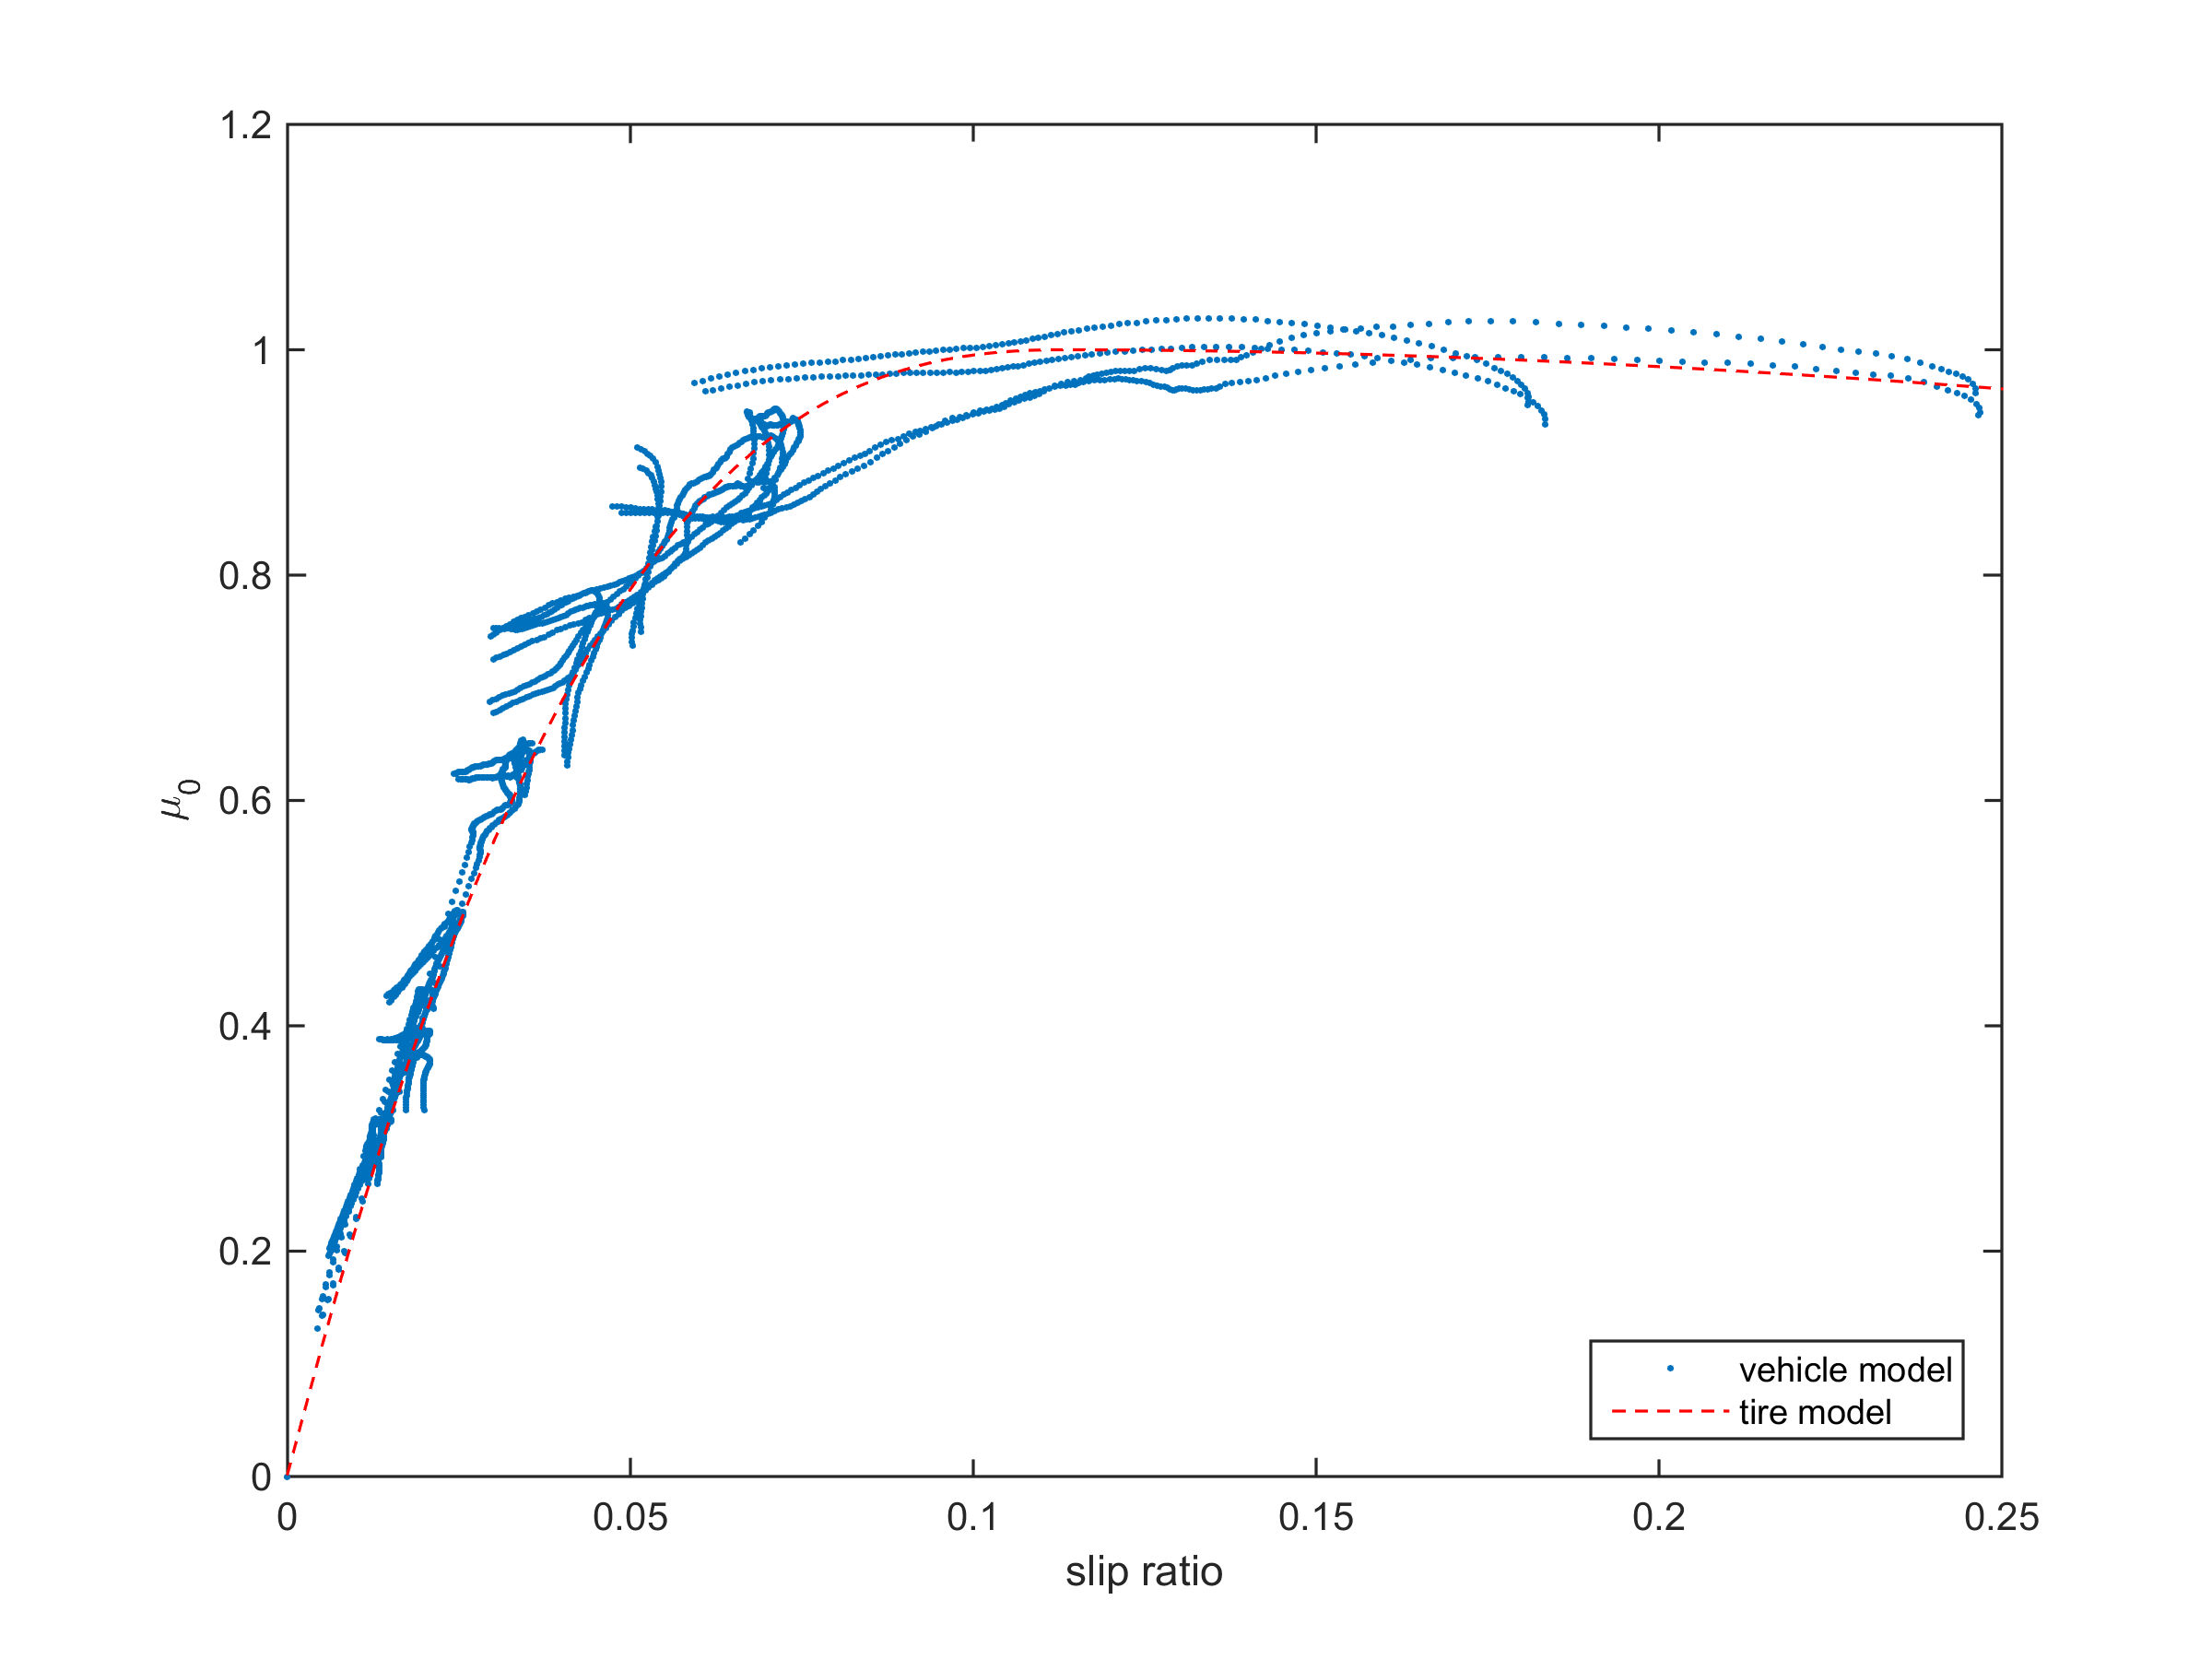
\includegraphics[width=0.8\textwidth]{Pictures/slip_kraft_ljungby}
	\caption {Normalized force per slip ratio for acceleration in a straight line with winter tires on asphalt.}
	\label{slip_kraft_ljungby}
\end{figure}

The tire model parameters that was fitted to the data and the friction coefficient became:
\begin{equation}
\label{winter_asphalt}
\begin{split}
C_{x} = 24 \\
\xi = 0.9 \\
\mu = 1.0 \\
\end{split}
\end{equation}
In Figure \ref{slip_kraft_is} the force per slip can be seen during a driving sequence on ice/snow. This driving sequence was made on a track and not merely an acceleration in a straight line. The effect of this is more variance in the vehicle force calculation compared to the result in Figure \ref{slip_kraft_ljungby}. 

\begin{figure}[h]
	\centering
	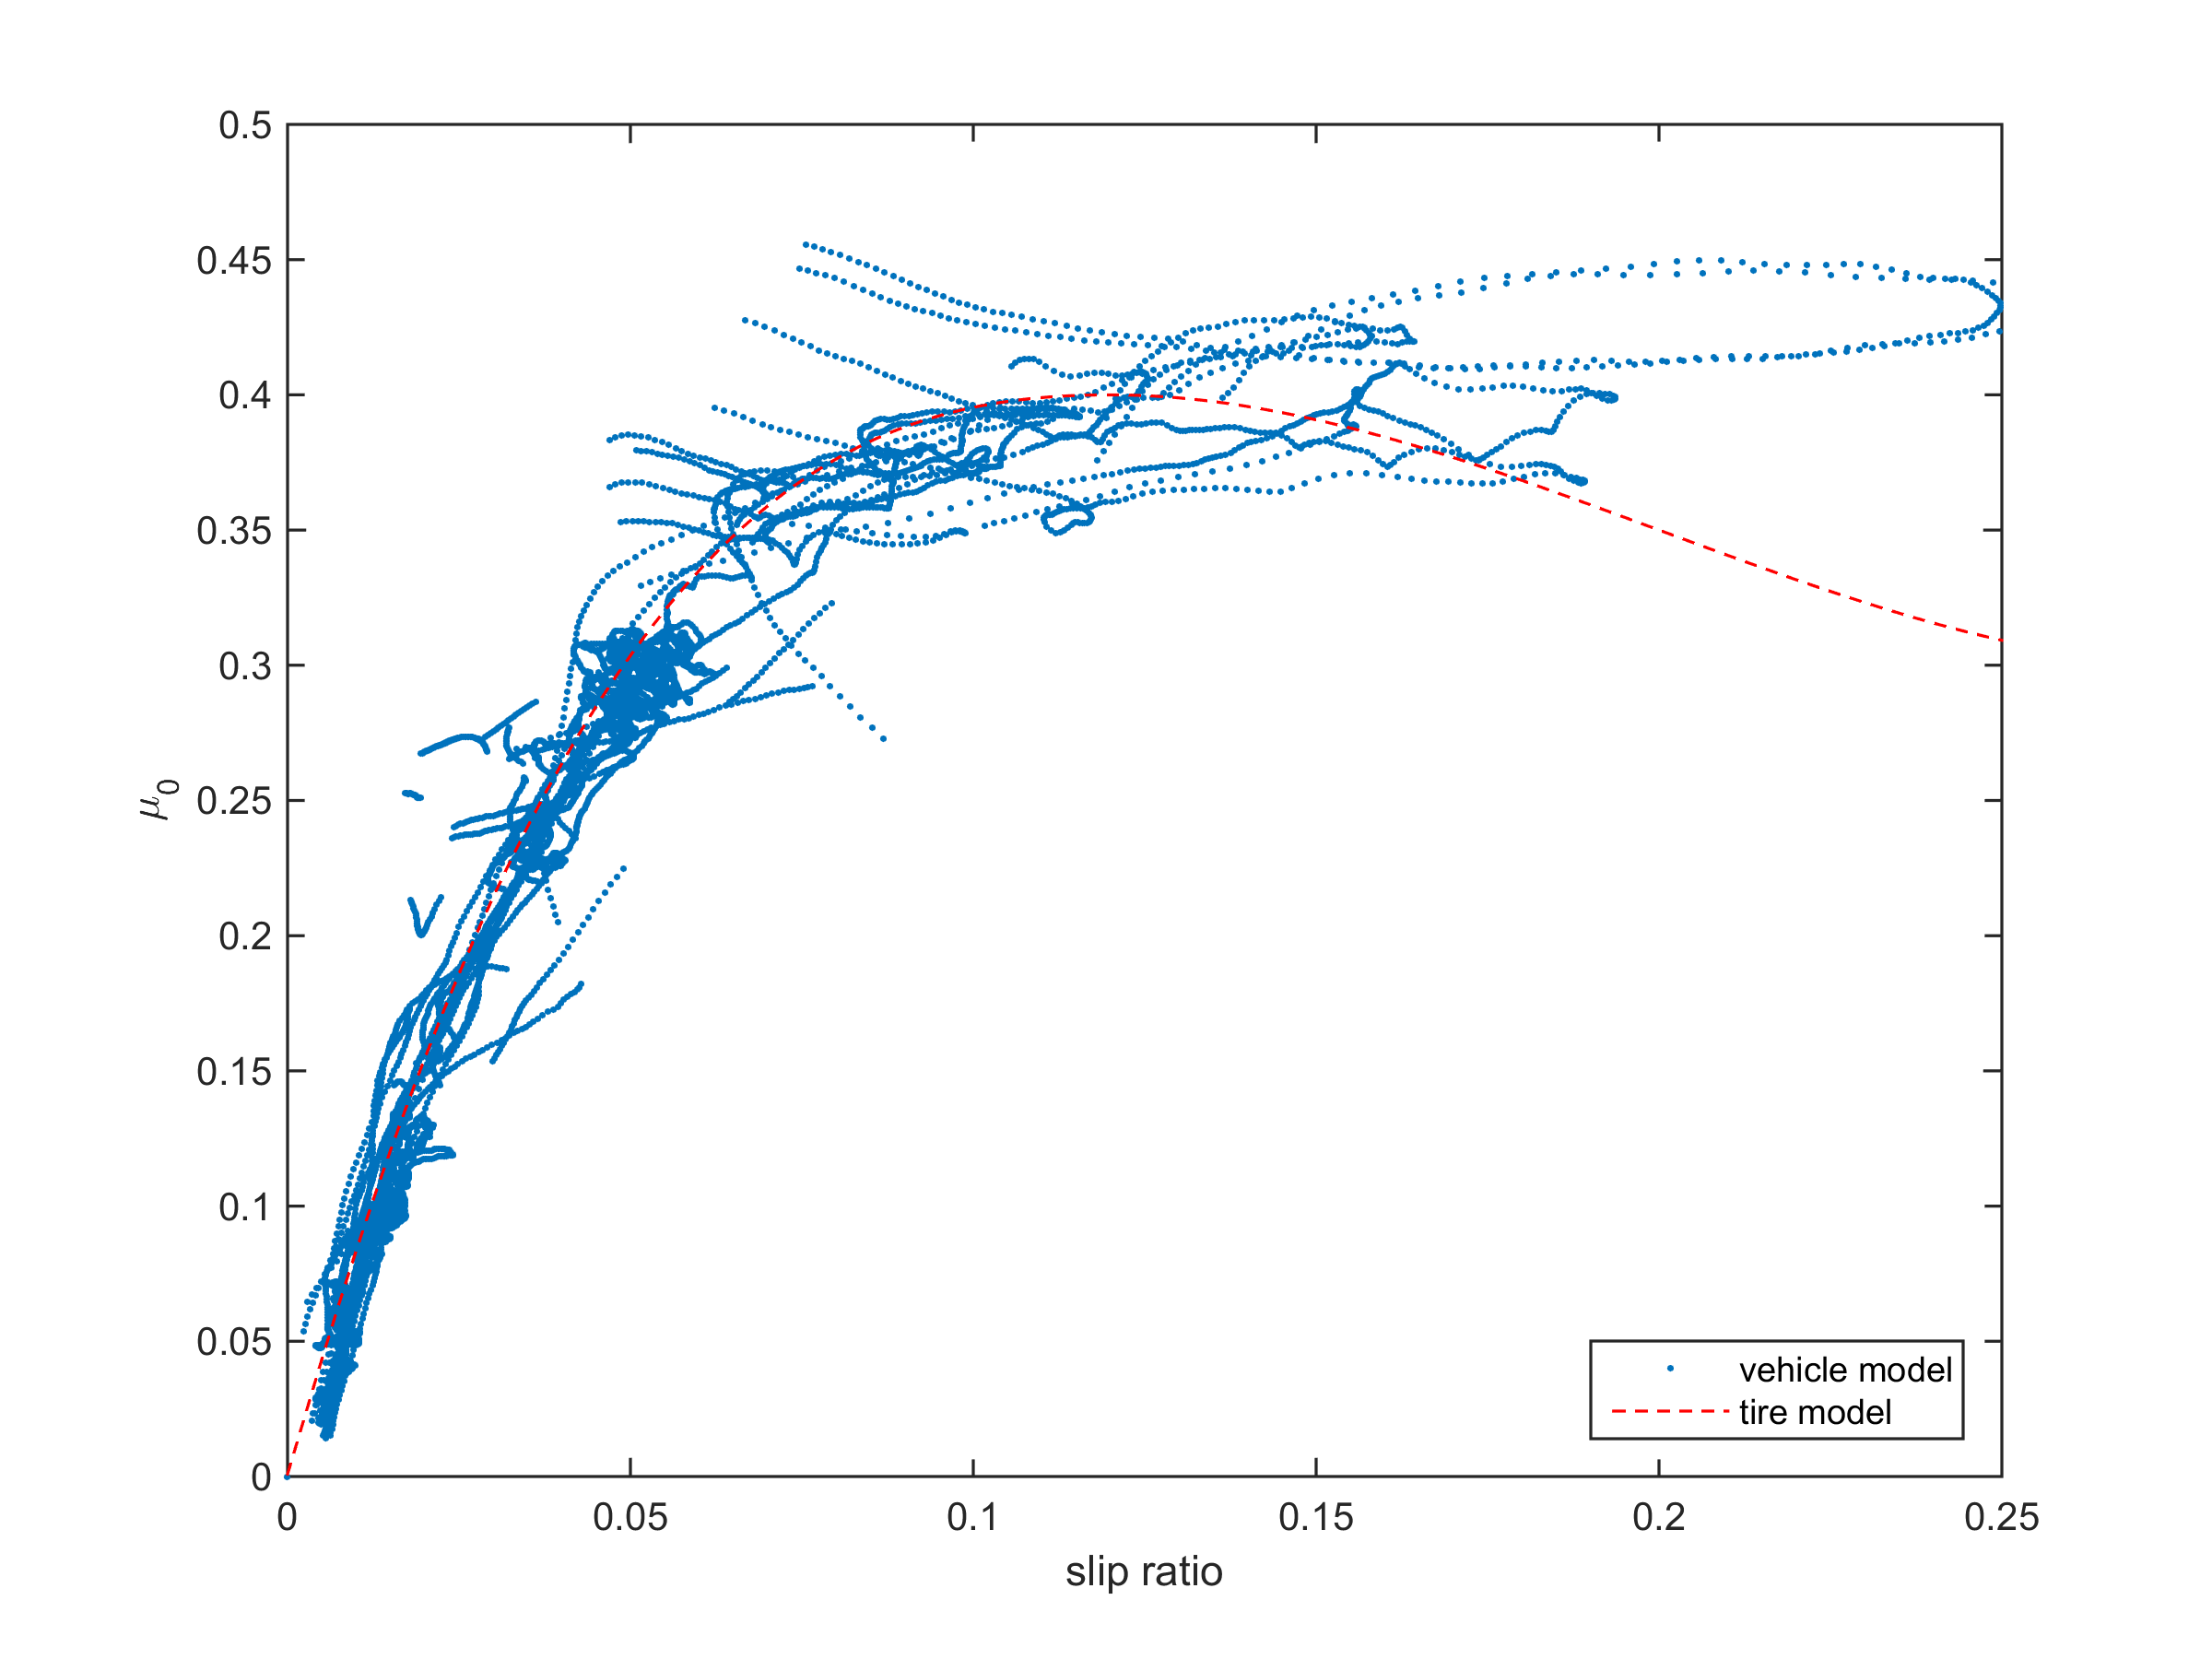
\includegraphics[width=0.8\textwidth]{Pictures/slip_kraft_is}
	\caption {Normalized force per slip ratio for a track run on ice/snow with winter tires.}
	\label{slip_kraft_is}
\end{figure}

The parameters for the fitted tire model and the friction coefficient for the ice driving sequence became:
\begin{equation}
\label{winter_ice}
\begin{split}
C_{x} = 9.5 \\
\xi = 0.9 \\
\mu = 0.4 \\
\end{split}
\end{equation}

To get the correct tire stiffness for different friction coefficient, a straight line was fitted between $ C_{x} $ and $ \mu $ in Figure \ref{winter_asphalt} and \ref{winter_ice}. This first degree fitting results in:
\begin{equation}
	C_{x} = 25\mu - 1
\end{equation}

\subsection{Summer tires}
\label{summer_tire}
Test driving has also been made with a set of summer tires on asphalt. The tires used were low profile tires which generally means high stiffness, i.e. low slip ratio values are needed to acquire the same longitudinal force, which can be seen in Figure \ref{slip_kraft_lk_sport}. The data acquired from this driving sequence does not include a lot of slip around the peak slip ratio, much due to the high stiffness and good grip from the low profile tires. It is only in the first gear that the slip ratio actually exceeds this peak in force which is assumed to be at slip ratio $ ~ 6 \% $.

The parameters for the fitted tire model and the friction coefficient for this asphalt driving sequence became:
\begin{equation}
\label{summer_lk}
\begin{split}
C_{x} = 38 \\
\xi = 0.7 \\
\mu = 1.15 \\
\end{split}
\end{equation}

\begin{figure}[h]
	\centering
	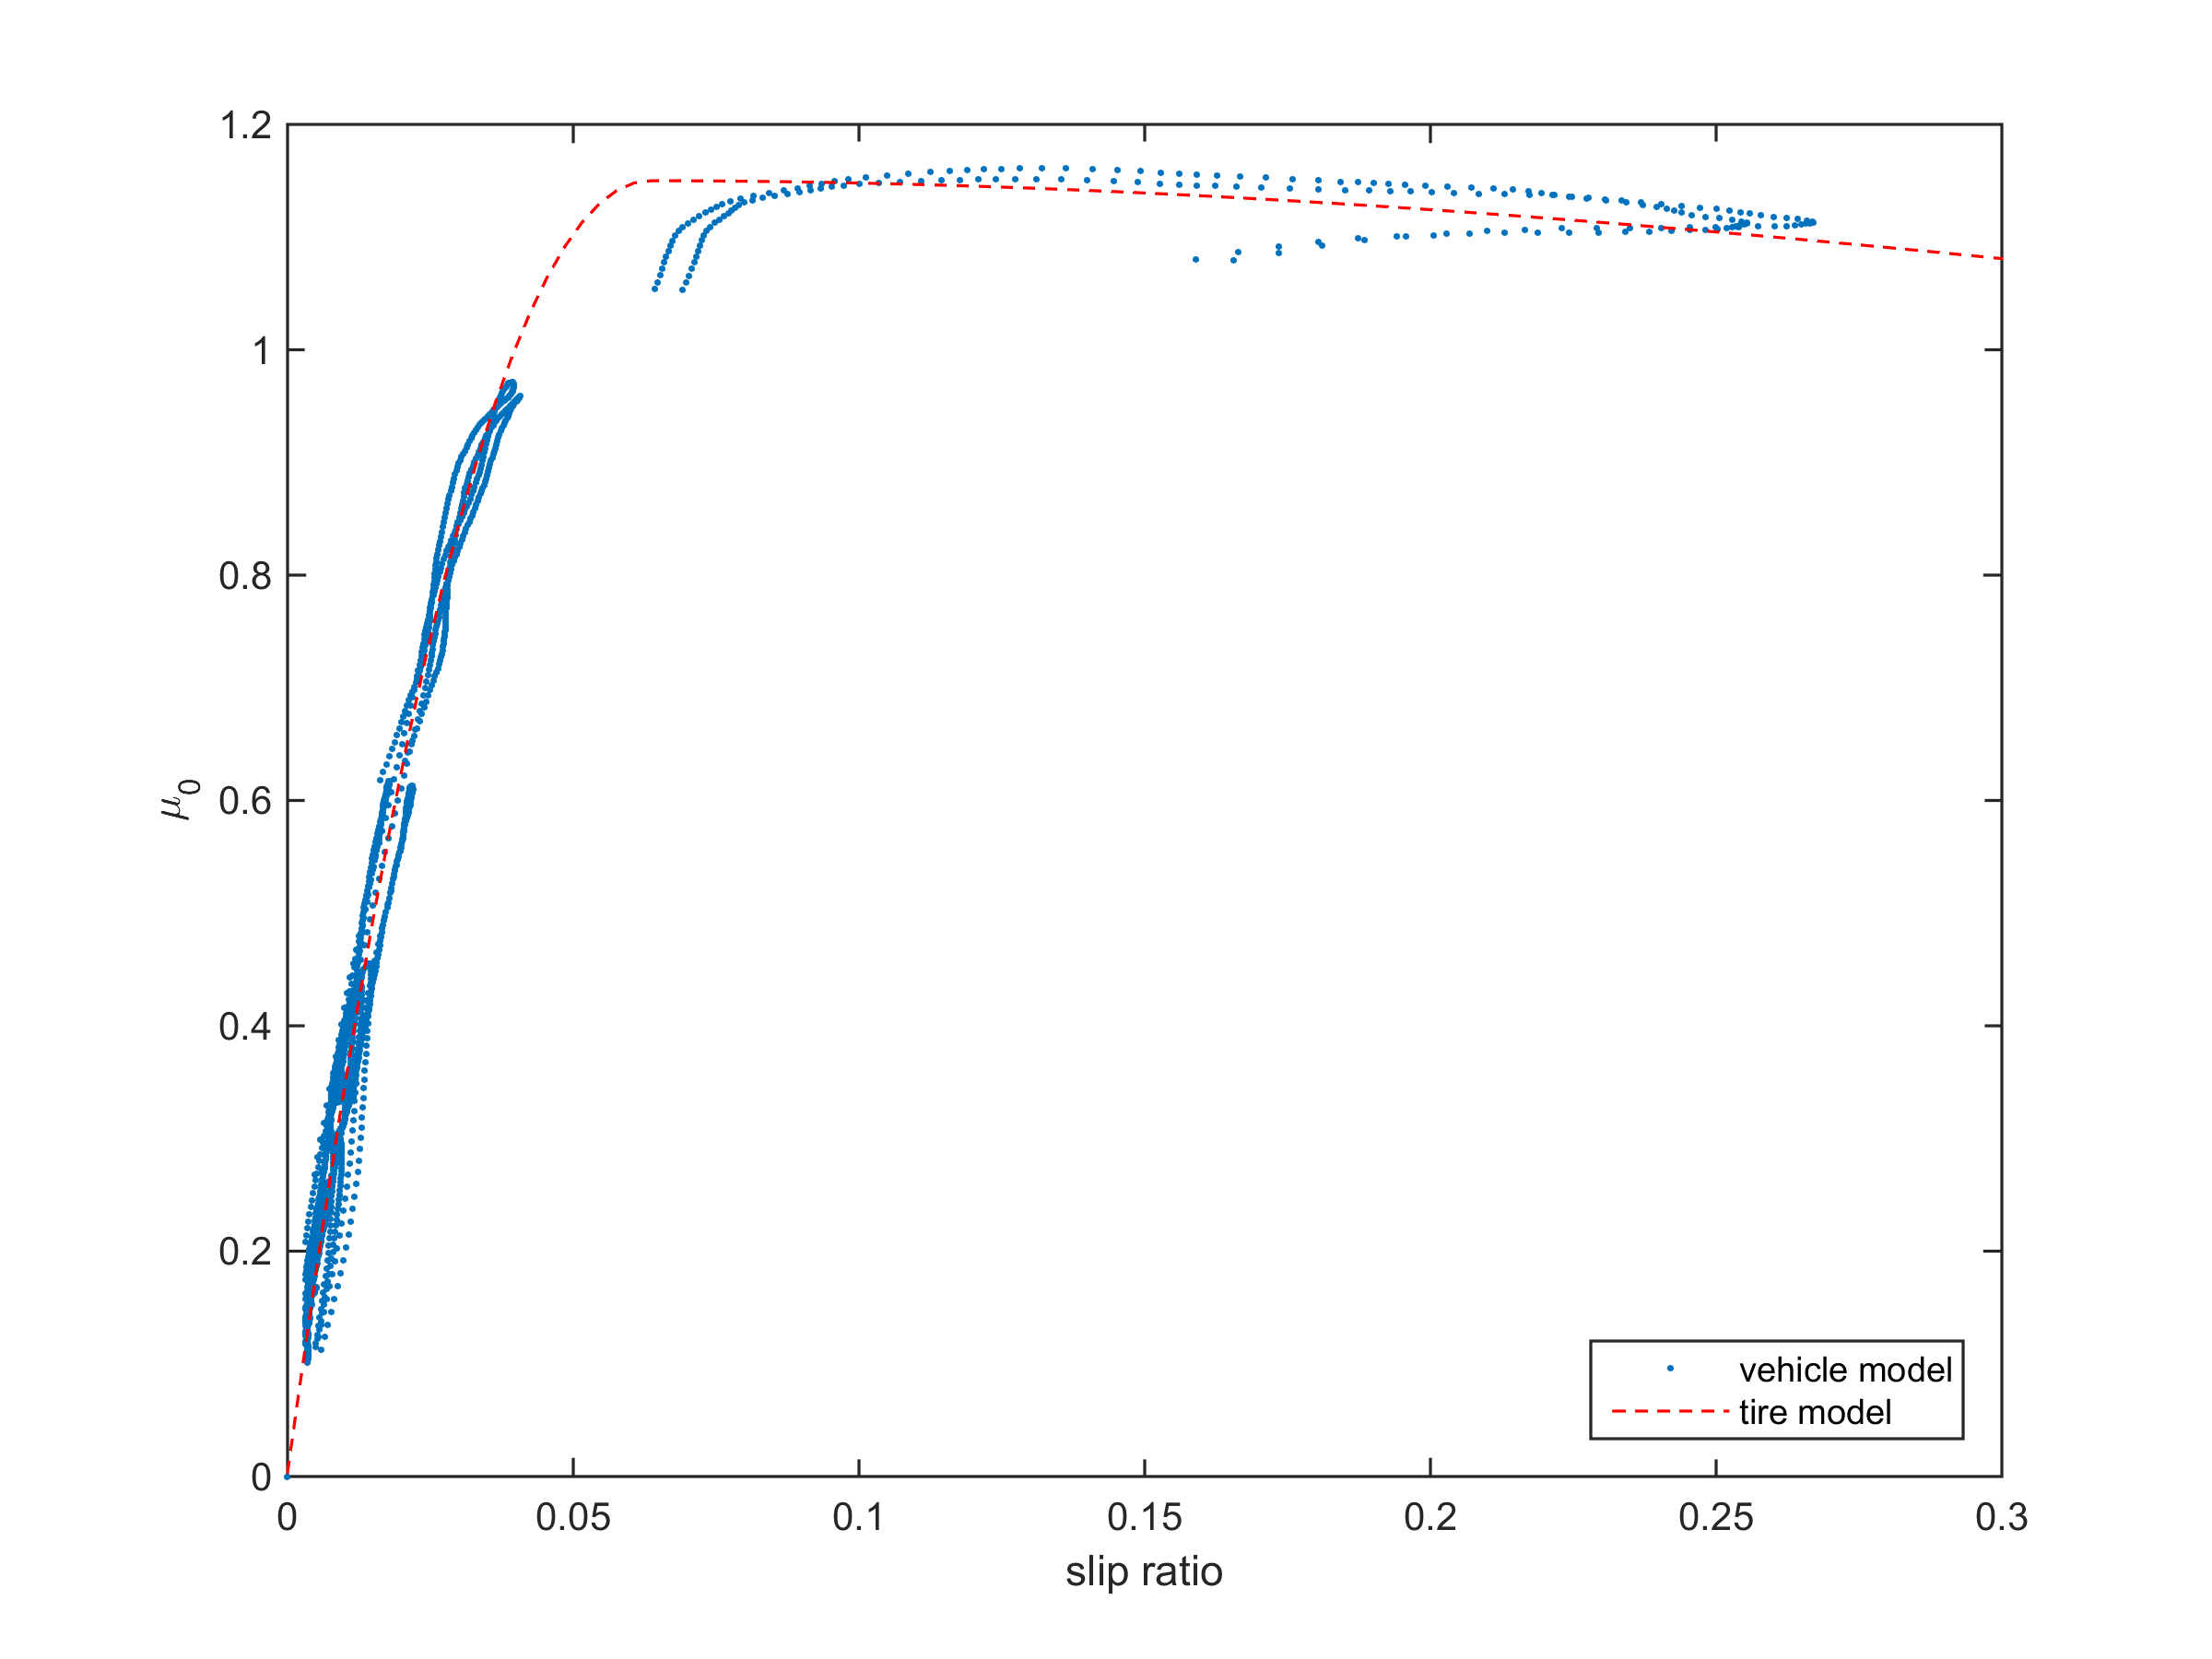
\includegraphics[width=0.8\textwidth]{Pictures/slip_kraft_lk_sport}
	\caption {Normalized force per slip ratio for acceleration in a straight line with summer tires on asphalt.}
	\label{slip_kraft_lk_sport}
\end{figure}

\subsection{Lateral acceleration compensation}
\label{sec:latacccomp}
The force per slip curves seen in Figure \ref{slip_kraft_ljungby} and \ref{slip_kraft_bb_torr}, where the tire model parameters are fitted, are derived from data acquired from merely accelerations done on a straight line. This means that no lateral forces are acting on the tires, which is very ideal conditions and unlikely during real driving sequences. When a vehicle is turning, it will also have a slip angle between the tires heading and pointing direction. When slip angle is present, the amount of longitudinal force actually generated per slip ratio will becomes less, see the curves for different slip angles in Figure \ref{combined}. However, slip angle is a parameter which is hard to approximate, and assumed to be unknown in this report. A parameter that is correlated to slip angle is the lateral acceleration., which means that it is most likely that lateral acceleration is present when a slip angle is. 
 
An approximation for the new slip ratio that is to be used is derived by:
\begin{equation}
\label{slip_ratio_compensation}
\kappa_{a_{y} compensated} = \dfrac{\kappa}{1 + a_{y}\cdot \beta}
\end{equation}
Where $ \beta $ represent how much the lateral acceleration should be considered. In Figure \ref{latacc_compensated}, two different force per slip ratio curves can be seen for a driving sequence which include cornering at high speeds, meaning that slip angle as well as lateral acceleration is present. The data is taken from a driving sequence using the same winter tires as seen in Figure \ref{slip_kraft_ljungby}, and therefore also using its fitted tire model parameters from Equation \ref{winter_asphalt}. In the first subplot of Figure \ref{latacc_compensated}, no compensation for lateral acceleration is considered, while the data in the second subplot uses the new approximated slip ratio derived by Equation \ref{slip_ratio_compensation} using $ \beta = 0.15 $. 
\begin{figure}[h]
	\centering
	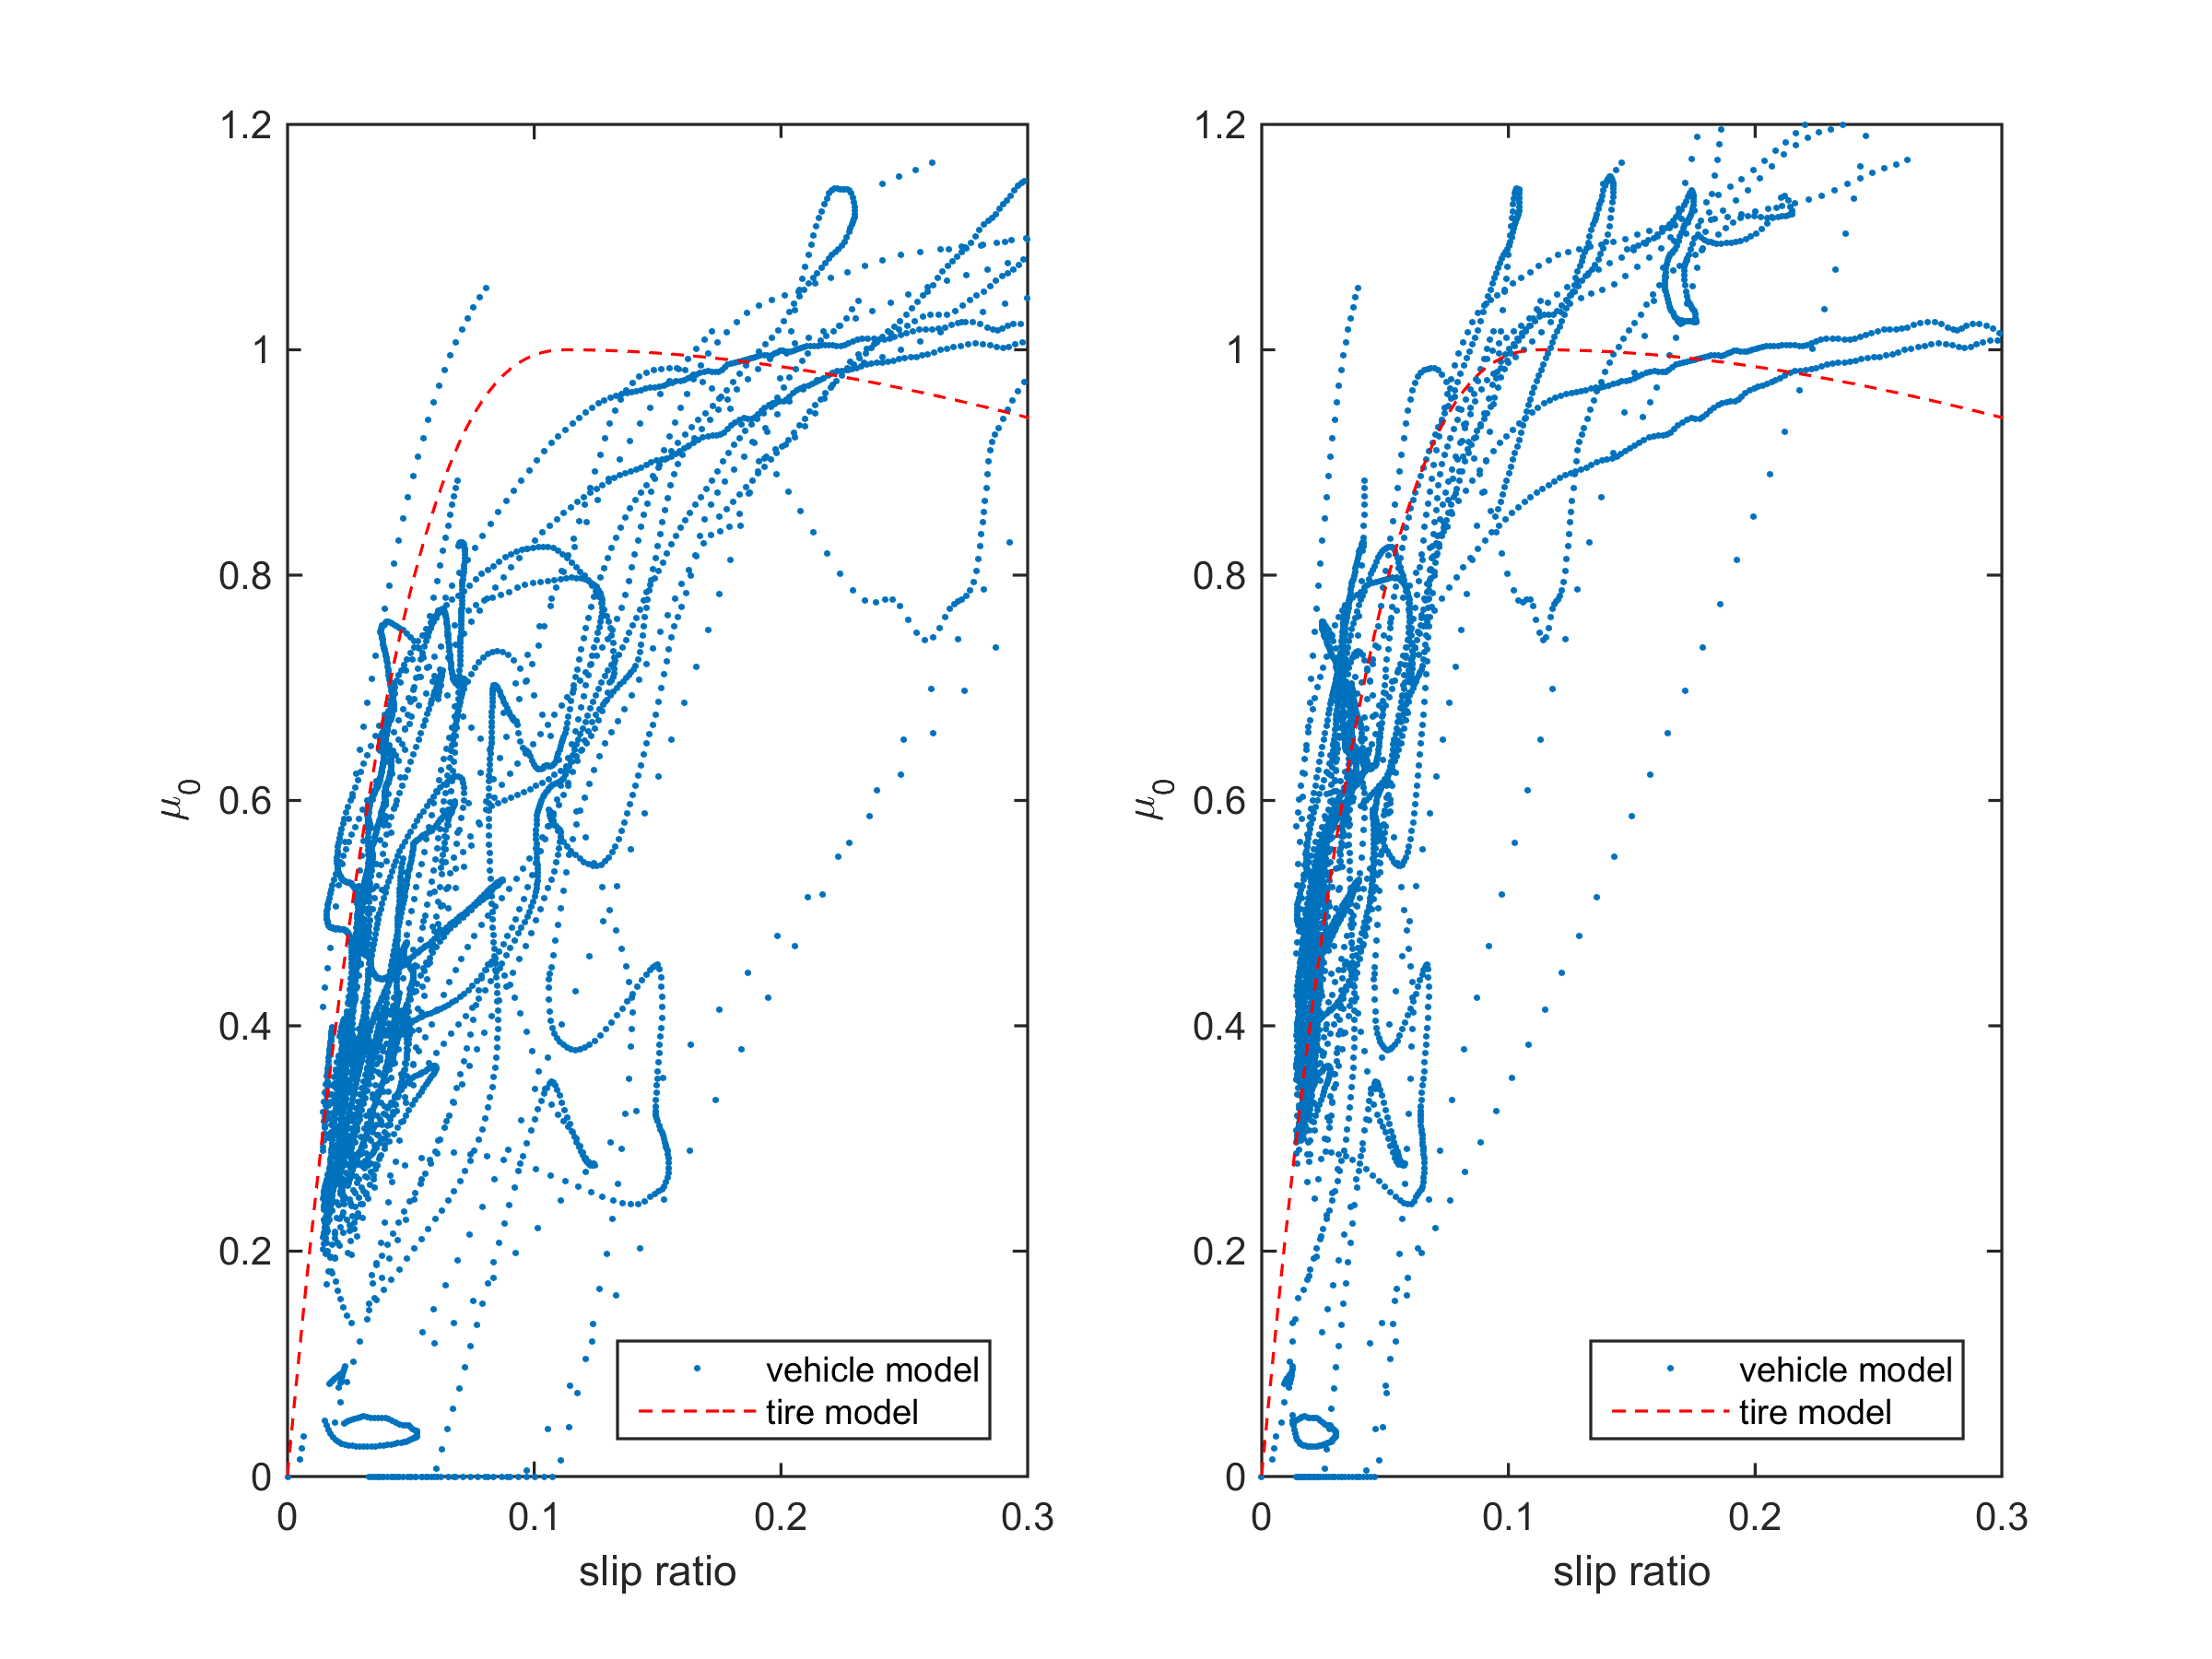
\includegraphics[width=1.0\textwidth]{Pictures/latacc_compensated}
	\caption {Normalized force per slip ratio when slip ratio is compensated due to lateral acceleration.}
	\label{latacc_compensated}
\end{figure}

\subsection{Tire mode selector}
The two different fitted tire models presented in \ref{winter_tire} and \ref{summer_tire} can result in very differing forces at the same slip ratio value. The tires that are used therefore need to be known in order for the system to work. It should also not be a necessity for the driver to specify what kind of tires that are used. The tire mode selector consist of an algorithm that finds the set of tire model parameters that matches the force from the vehicle model with the smallest error. The algorithm calculates the force difference between the respective set of tire parameters and the vehicle model and thereafter low pass filters the result with a slowly acting filter, so that sudden changes does not affect what tire parameters to use. 

\section{Estimating the friction coefficient}
The aim om the friction estimation is, as mentioned earlier, to choose the correct friction coefficient so that the forces from the two different models become alike. In other words, choose the $ \mu $ that enables:
\begin{equation}
	F_{vehicle} = F_{tire}
\end{equation}
This relation, and therefore also a friction coefficient, could theoretically be obtained at every instance when new CAN packages are available. This would lead to a rapid changing friction coefficient which wouldn't reflect the actual tire/road friction. Instead of approximating a new friction coefficient at every moment, a least square fitting method is used to find the friction coefficient. The goal of such a method is to find the friction coefficient that provides the smallest error between the two models over a certain amount of time. 

\subsection{Least square fitting}
The general idea of a least square fitting method is to minimize the sum of the squares between a theoretical model and observed data. 
\begin{equation} 
	y(k) = \phi(k)\cdot\theta + v
	\label{eq:least_square}
\end{equation}
Where $ y $ is the observed data, $ \phi(k)\cdot\theta $ the theoretical model and $ v $ the error. The cost function that should be minimized becomes the following:
\begin{equation}
	V(\hat{\theta}, k) = \dfrac{1}{2} \sum_{i=1}^{k} \lambda^{k-i}\Big(y(i) - \phi(i)\cdot\hat\theta \Big)^2
\end{equation}
Due to the fact that new data is acquired continuously, these least square approximations would need to be executed at every time step, creating unreasonable amount of computations. Hence, a modification of the least square fitting is used which recursively takes previous results into account.

\subsection{Recursive least square fitting}
The recursive least square (RLS) fitting method is defined as:
\begin{equation}
	L(k) =\dfrac{ P(k-1)\phi (k)}{\lambda + \phi (k) P(k-1)\phi(k)} 
\label{eq:RLS1}
\end{equation}
\begin{equation}
	P(k) = \Big( 1 - L(k)\phi (k) \Big) \dfrac{1}{\lambda} P(k-1)
\label{eq:RLS2}
\end{equation}
\begin{equation}
\hat \theta (k) = \hat \theta (k-1) + L(k) \cdot v(k)
\label{eq:RLS3}
\end{equation}
Where the error is:
\begin{equation}
	v(k) = y(k) - \phi (k) \hat \theta (k-1)
	\label{eq:RLS4}
\end{equation}
L and P define how much the next $ \theta $ update should rely on the error. A larger L takes the error into account more, while a smaller number makes the update rely on the old $ \theta $ value more. The forgetting factor, $ \lambda $, is defined by the user and basically describes how many previous values to consider when calculating a new $ \theta $.

However, this method can only be applied to linear system, and a tire force, $F=f(\kappa, Fz, \mu, C_{x})$, is not linear. To able to use the RLS, the function has to be linearized. To accomplish this, the derivative of the force as a function of $ \mu $ is defined as:
\begin{equation}
	\dfrac{\partial F}{\partial \mu} = \dfrac{\partial f(\kappa, Fz, \mu, C_{x})}{\partial \mu}
\end{equation}
Which describes how much the force will increase dependent on $ \mu $. The force in that linearized region thereafter becomes:
\begin{equation}
	F_{vehicle} = \dfrac{\partial F_{tire}}{\partial \mu} \cdot \mu
\end{equation}
This function now has the same form as Equation \ref{eq:least_square}, which means that the RLS method in Equations \ref{eq:RLS1}-\ref{eq:RLS4} can be used. The RLS with its proper parameters is:
\begin{equation}
	L(k) =\dfrac{ P(k-1) \dfrac{\partial F_{tire}(k)}{\partial \mu}}{\lambda + \dfrac{\partial F_{tire}(k)}{\partial \mu} P(k-1) \dfrac{\partial F_{tire}(k)}{\partial \mu}} 
\end{equation}
\begin{equation}
	P(k) = \Bigg( 1 - L(k) \dfrac{\partial F_{tire}(k)}{\partial \mu} \Bigg) \dfrac{1}{\lambda} P(k-1)
\end{equation}
\begin{equation}
	\mu (k) = \mu (k-1) + L(k) \Big( F_{vehicle} (k) - F_{tire} (k) \Big)
\end{equation}
The friction coefficient value is updated every step and depends on its own value, the error between the vehicle and tire model, and the number L describing how much to rely on the error. $ \dfrac{\partial F_{tire}}{\partial \mu} $ becomes larger for slips close to the peak force, which means that larger changes of $ \mu $ is possible at that point. The forgetting factor, $ \lambda $, is usually a value in the region $ [0.9, 1) $, where a larger forgetting factor means that older values are considered more, resulting in slower changes of $ \mu $.

\subsection{When to estimate the friction coefficient}
In a perfect world, it would be desired to be able to estimate the friction coefficient during every driving situation in order to capture any sudden change of grip between the tire and the road that can be present. Unfortunately there exist many challenges during most driving sequences that have to be considered. During some situations, either the vehicle or the tire model are shown to capture the occurrence far from its reality. These situations need to be identified so that the RLS fitting method does not update the estimated friction coefficient value at these period of times. This means that the friction coefficient value will no be continuously updated throughout every driving sequence and that sudden changes of the tire/road friction can be missed.

\subsubsection{Limitations due to slip ratio }
There are a couple of driving sequences that affect the slip ratio in such a way that the forces cannot be modeled correctly. When braking, the slip ratio should be close to zero assuming braking forces on all tires, meaning that tire forces cannot be modeled. During cornering, the front wheels will be turned creating a lateral force and a yaw rate. The rear, which doesn't have any positive cornering effect, will follow the front wheels but in a smaller radius, leading to a lower velocity. This difference in velocity between the front and rear wheels will result in a slip ratio that is non proportional to the amount of force generated at the tires. This phenomena will be larger when cornering at low speeds, due to the fact that a smaller lateral force is acting, and therefore not pushing the rear axle to a larger radius. This large slip ratio due to cornering can be seen in Figure \ref{turning_slow_Vx}. At around $ 20 $ s and after $ 30 $ s, the vehicle is turning at a low speed. This results in a large slip ratio seen in the first subplot, which exists without adding a positive longitudinal force.

\begin{figure}[h]
	\centering
	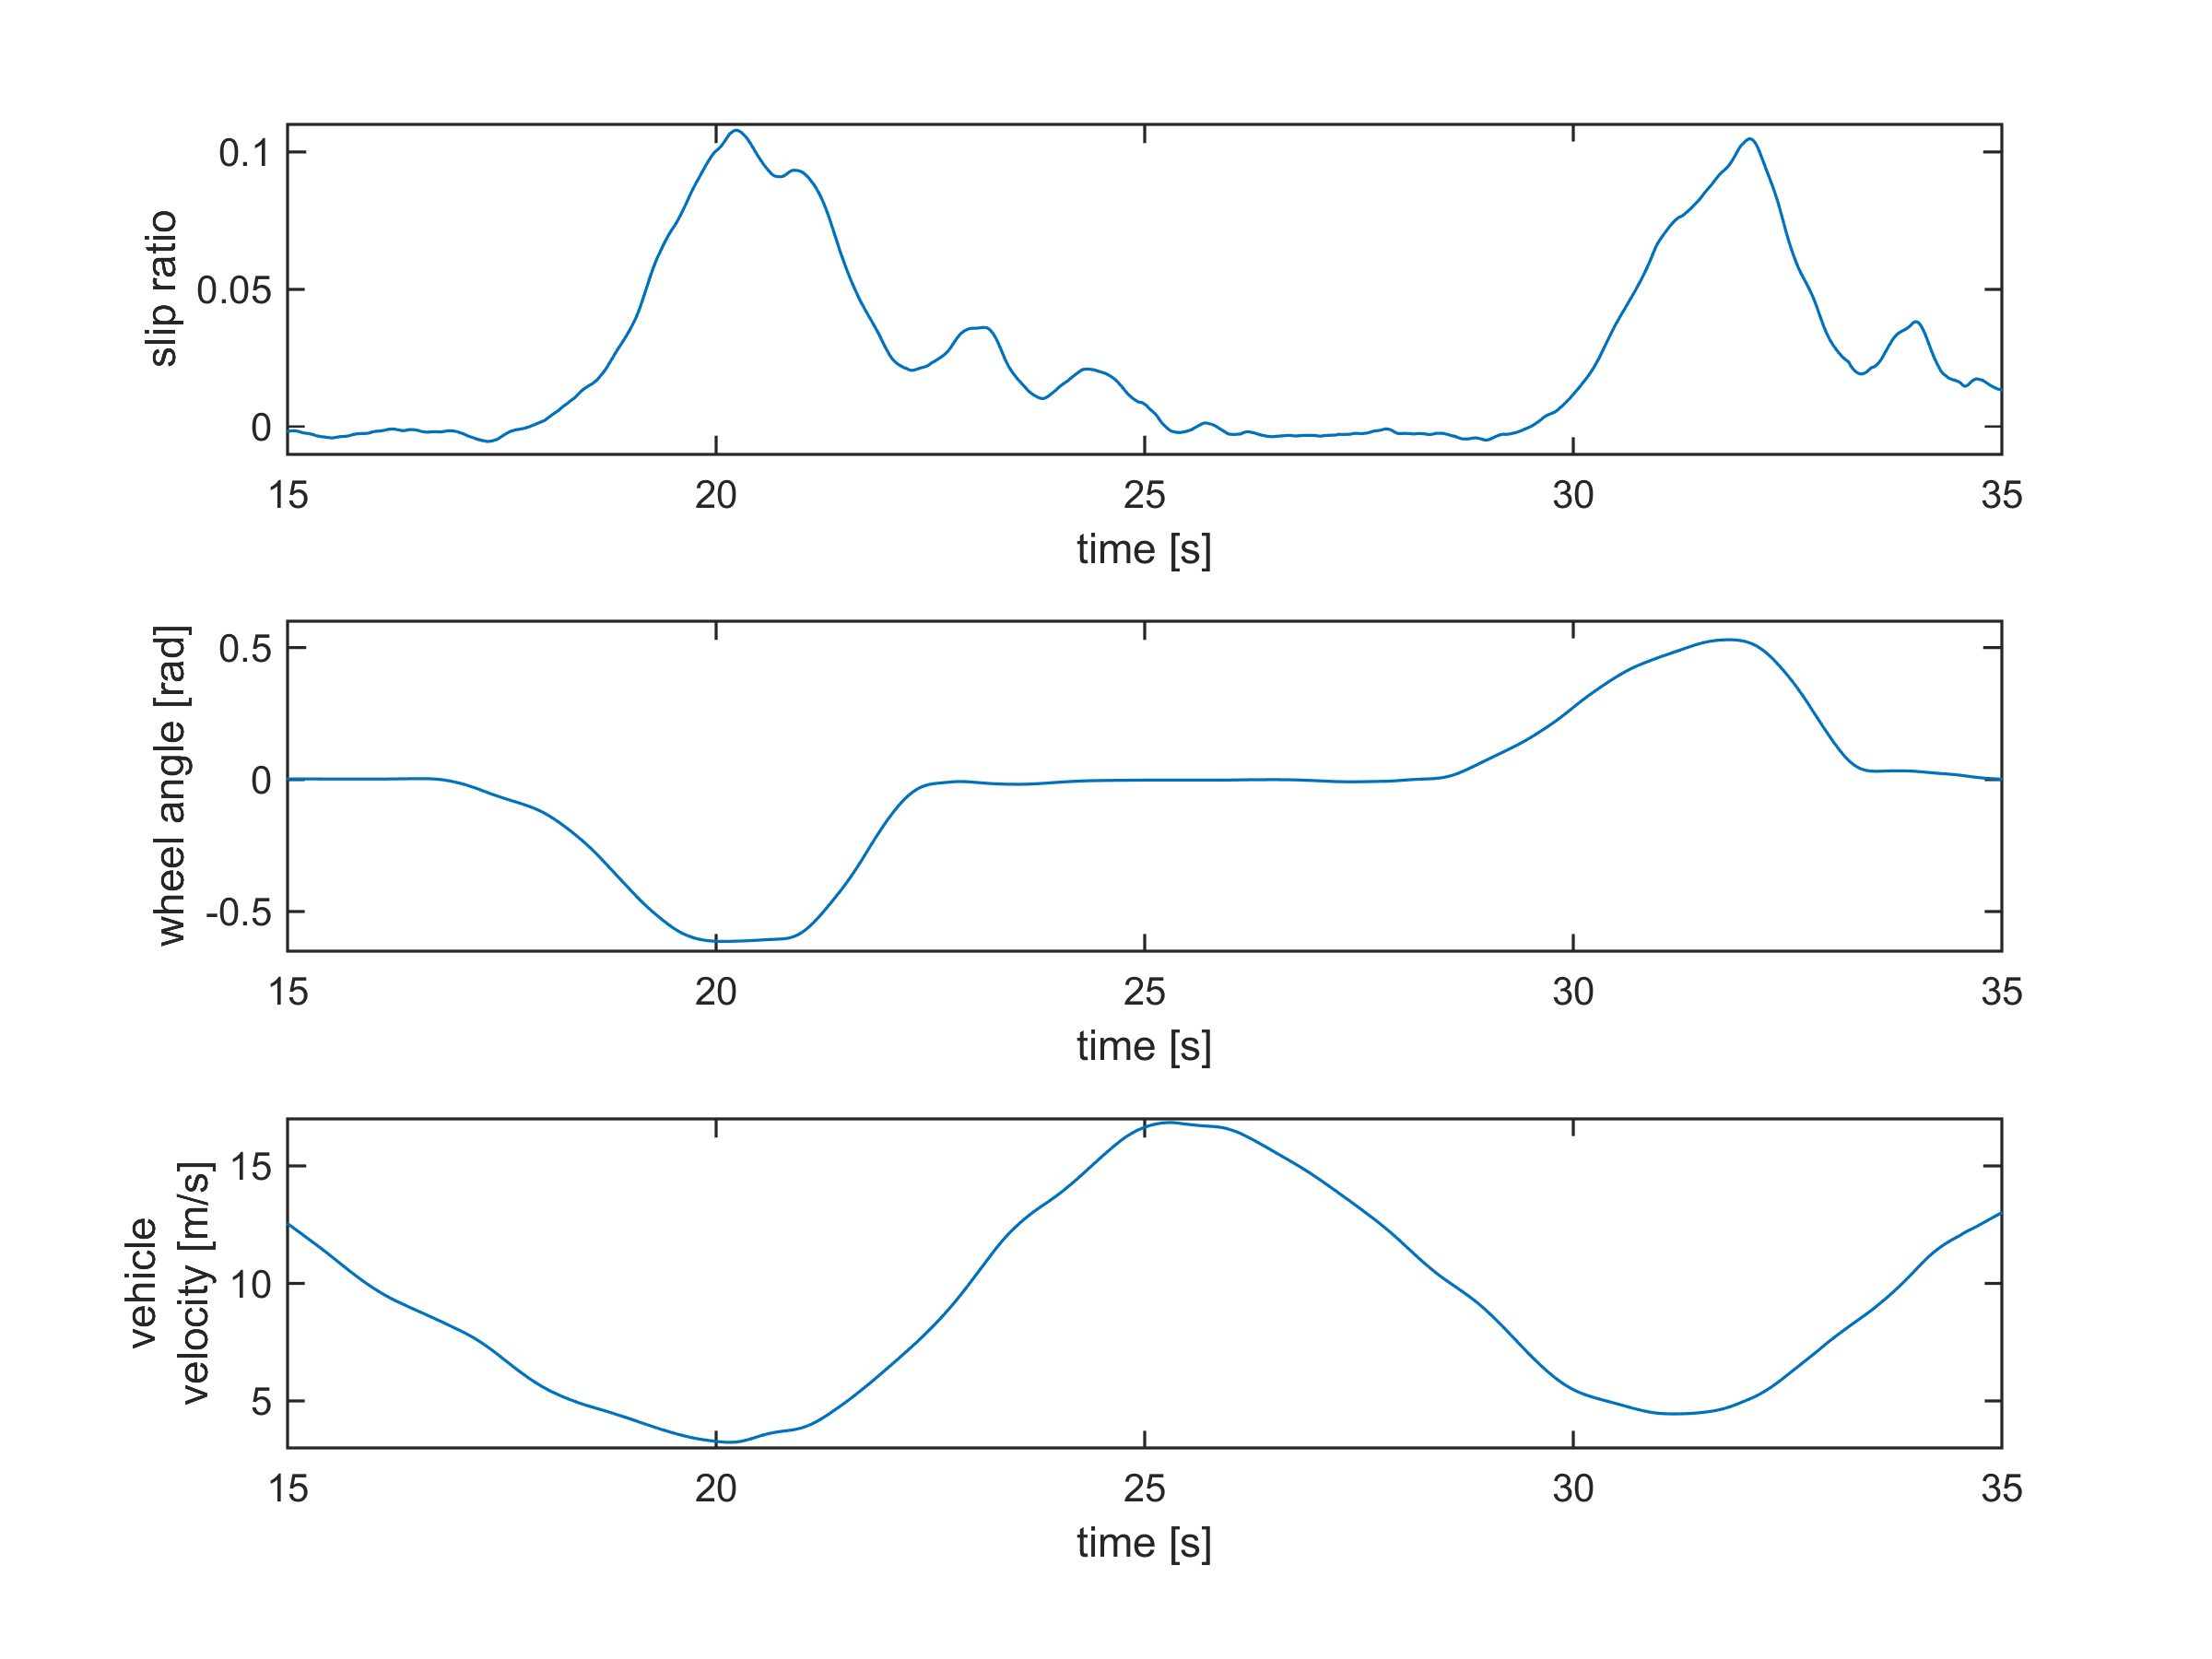
\includegraphics[width=1.0\textwidth]{Pictures/turning_slow_Vx}
	\caption {Large slip values are seen when cornering at a low velocity.}
	\label{turning_slow_Vx}
\end{figure}

Another driving scenario that creates a misleading slip ratio is during acceleration from standing still, which can be seen in Figure \ref{slipratio_from_still}, at around $ 2 $ s and $ 24 $ s. When the accelerate begins, the front wheels will start to turn slightly ahead compared to the rear wheels. The percentage difference between the two wheels will become large due to the low velocity, leading to an unreasonable high slip ratio. The same phenomena can also be seen in Figure \ref{slipratio_from_still} right before the vehicle comes to a stop, at around $ 22 $ s. 

\begin{figure}[h]
	\centering
	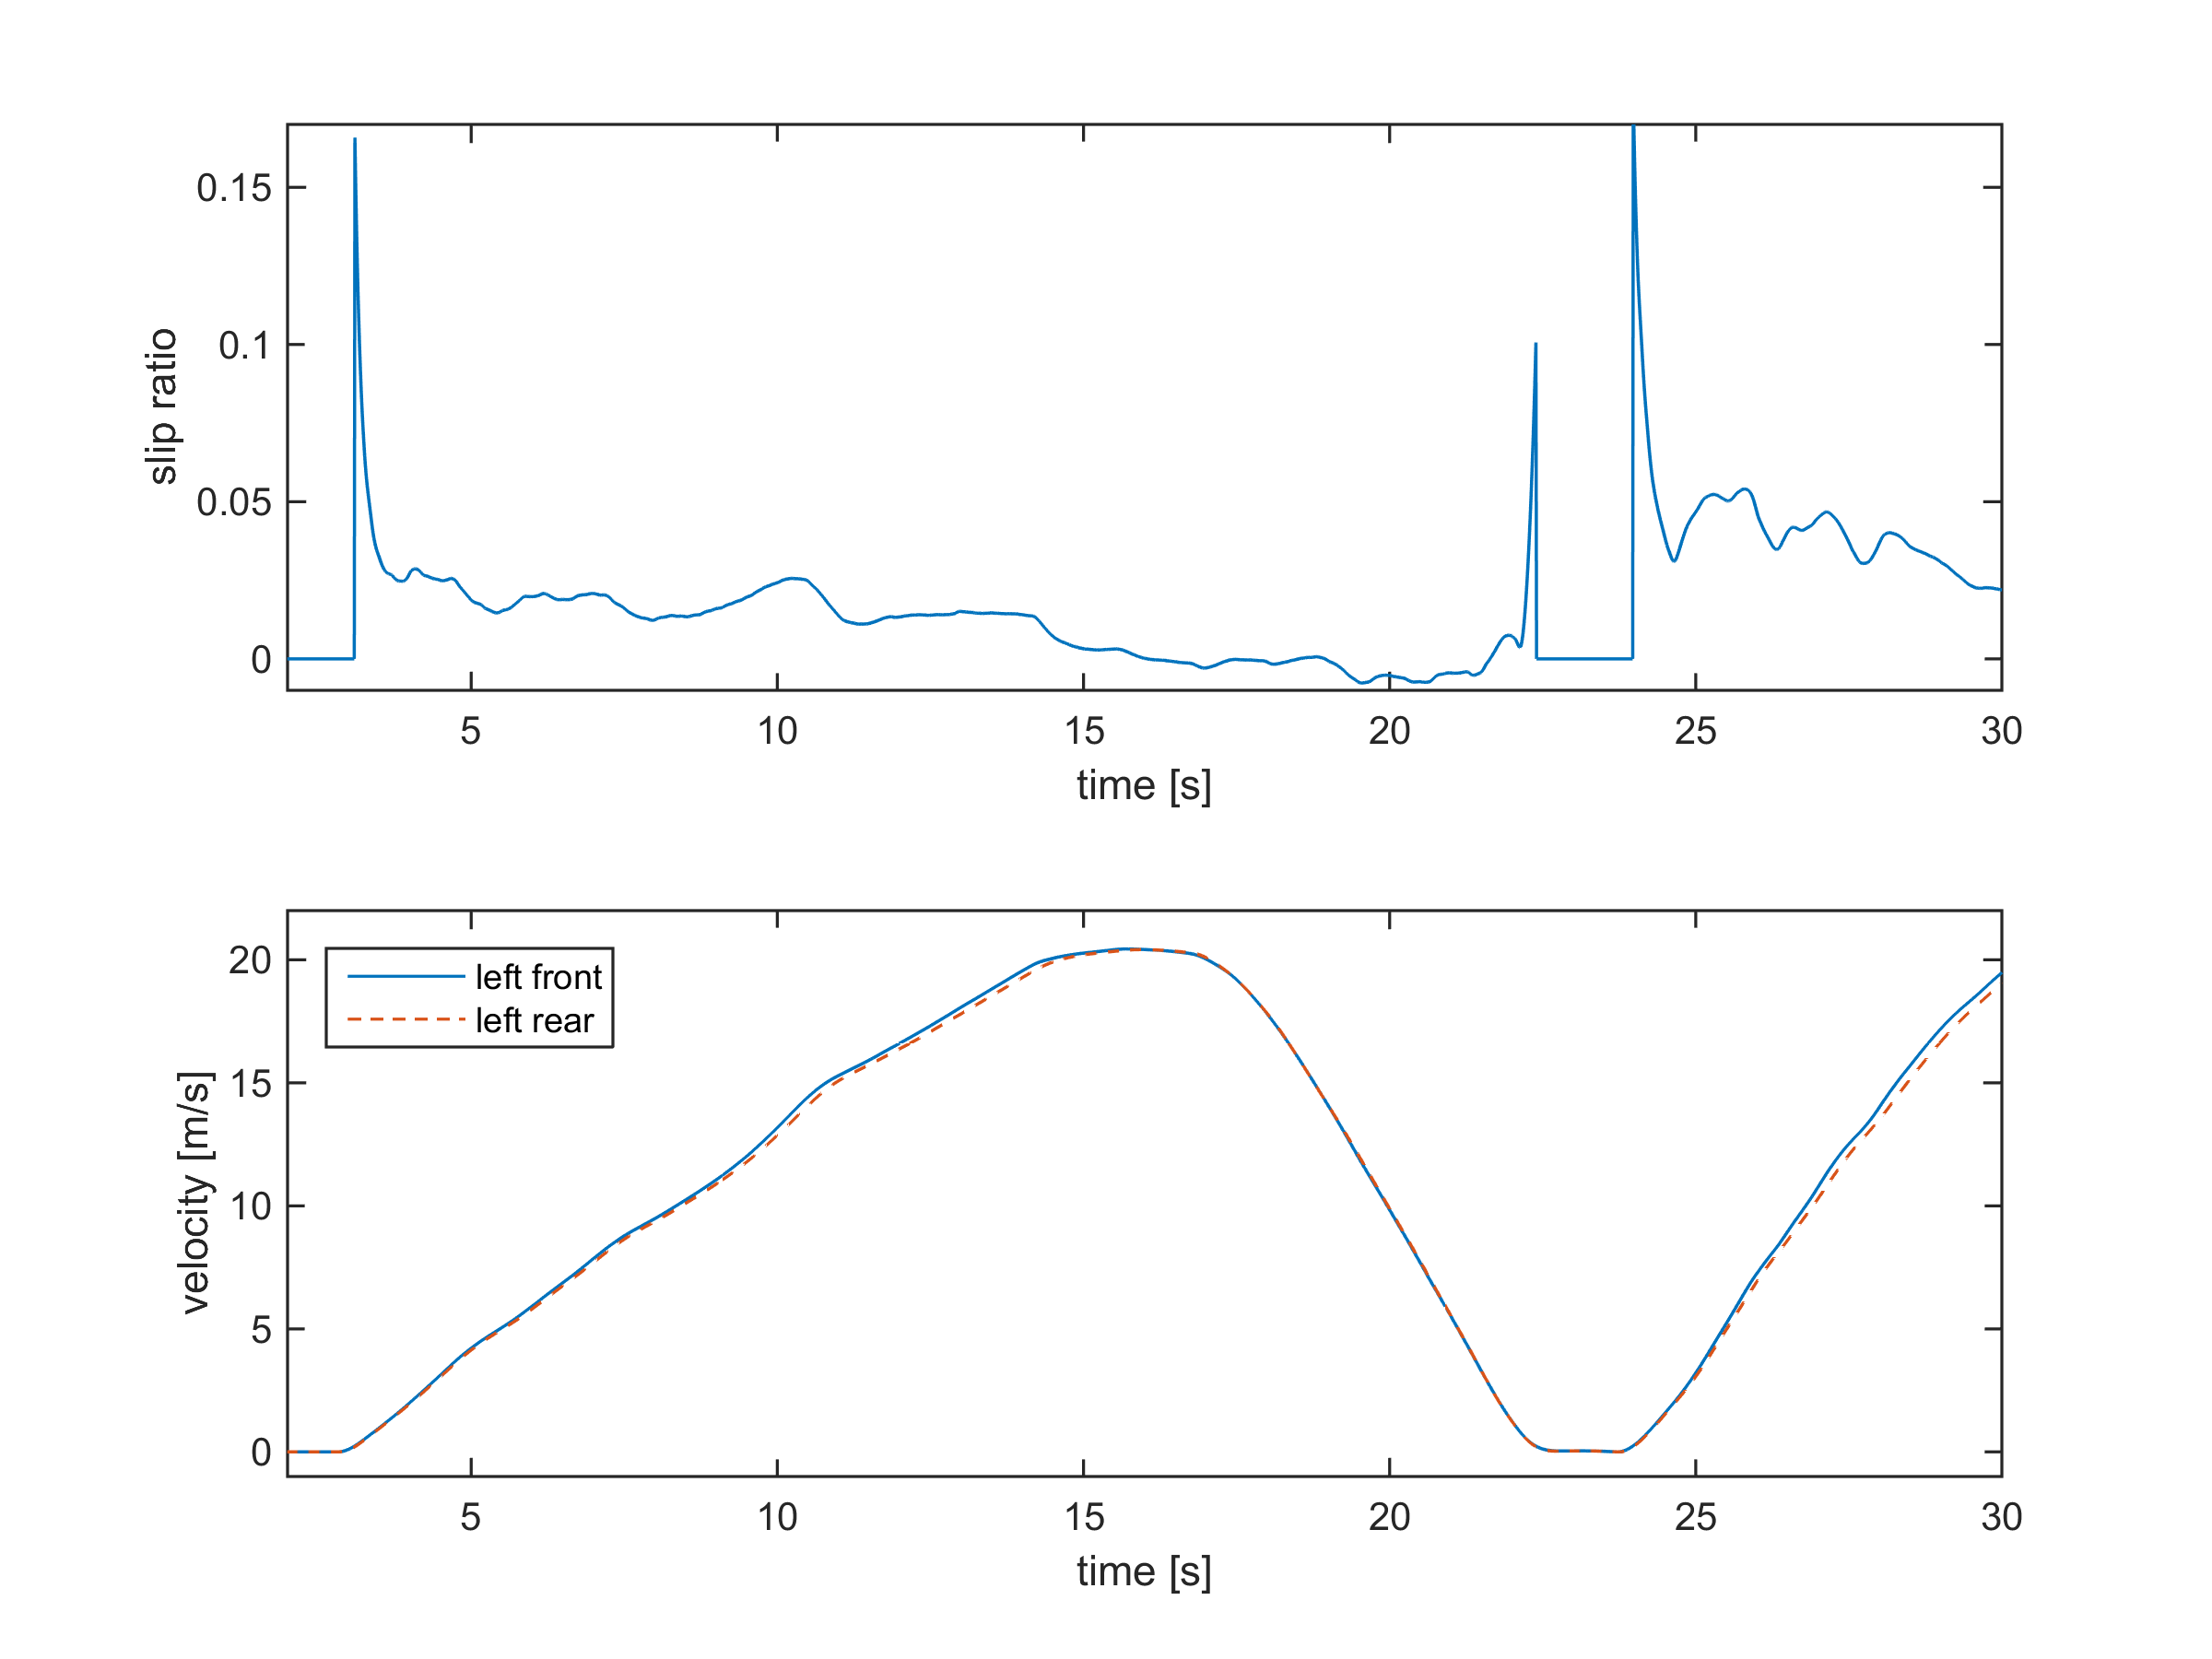
\includegraphics[width=1.0\textwidth]{Pictures/slipratio_from_still}
	\caption {Large slip values are seen when a vehicle begins an acceleration from standing still.}
	\label{slipratio_from_still}
\end{figure}

Limitations has to be set so that the RLS fitting method does not update the estimated friction coefficient at these presented scenarios when the calculated slip ratio gives an unreliable result.

\subsubsection{Limitations due to gear changes}
\label{sec:gearchange}
When a vehicle engages the clutch prior to a gear change, there will be no torque transfered from the engine out to the wheels. Due to filtering and differences between various signals, the force losses in the different models will be different. This can be seen in Figure \ref{gear_change}, where gear changes appear at around $ 54.5 $ s and $ 57 $ s.

\begin{figure}[h]
	\centering
	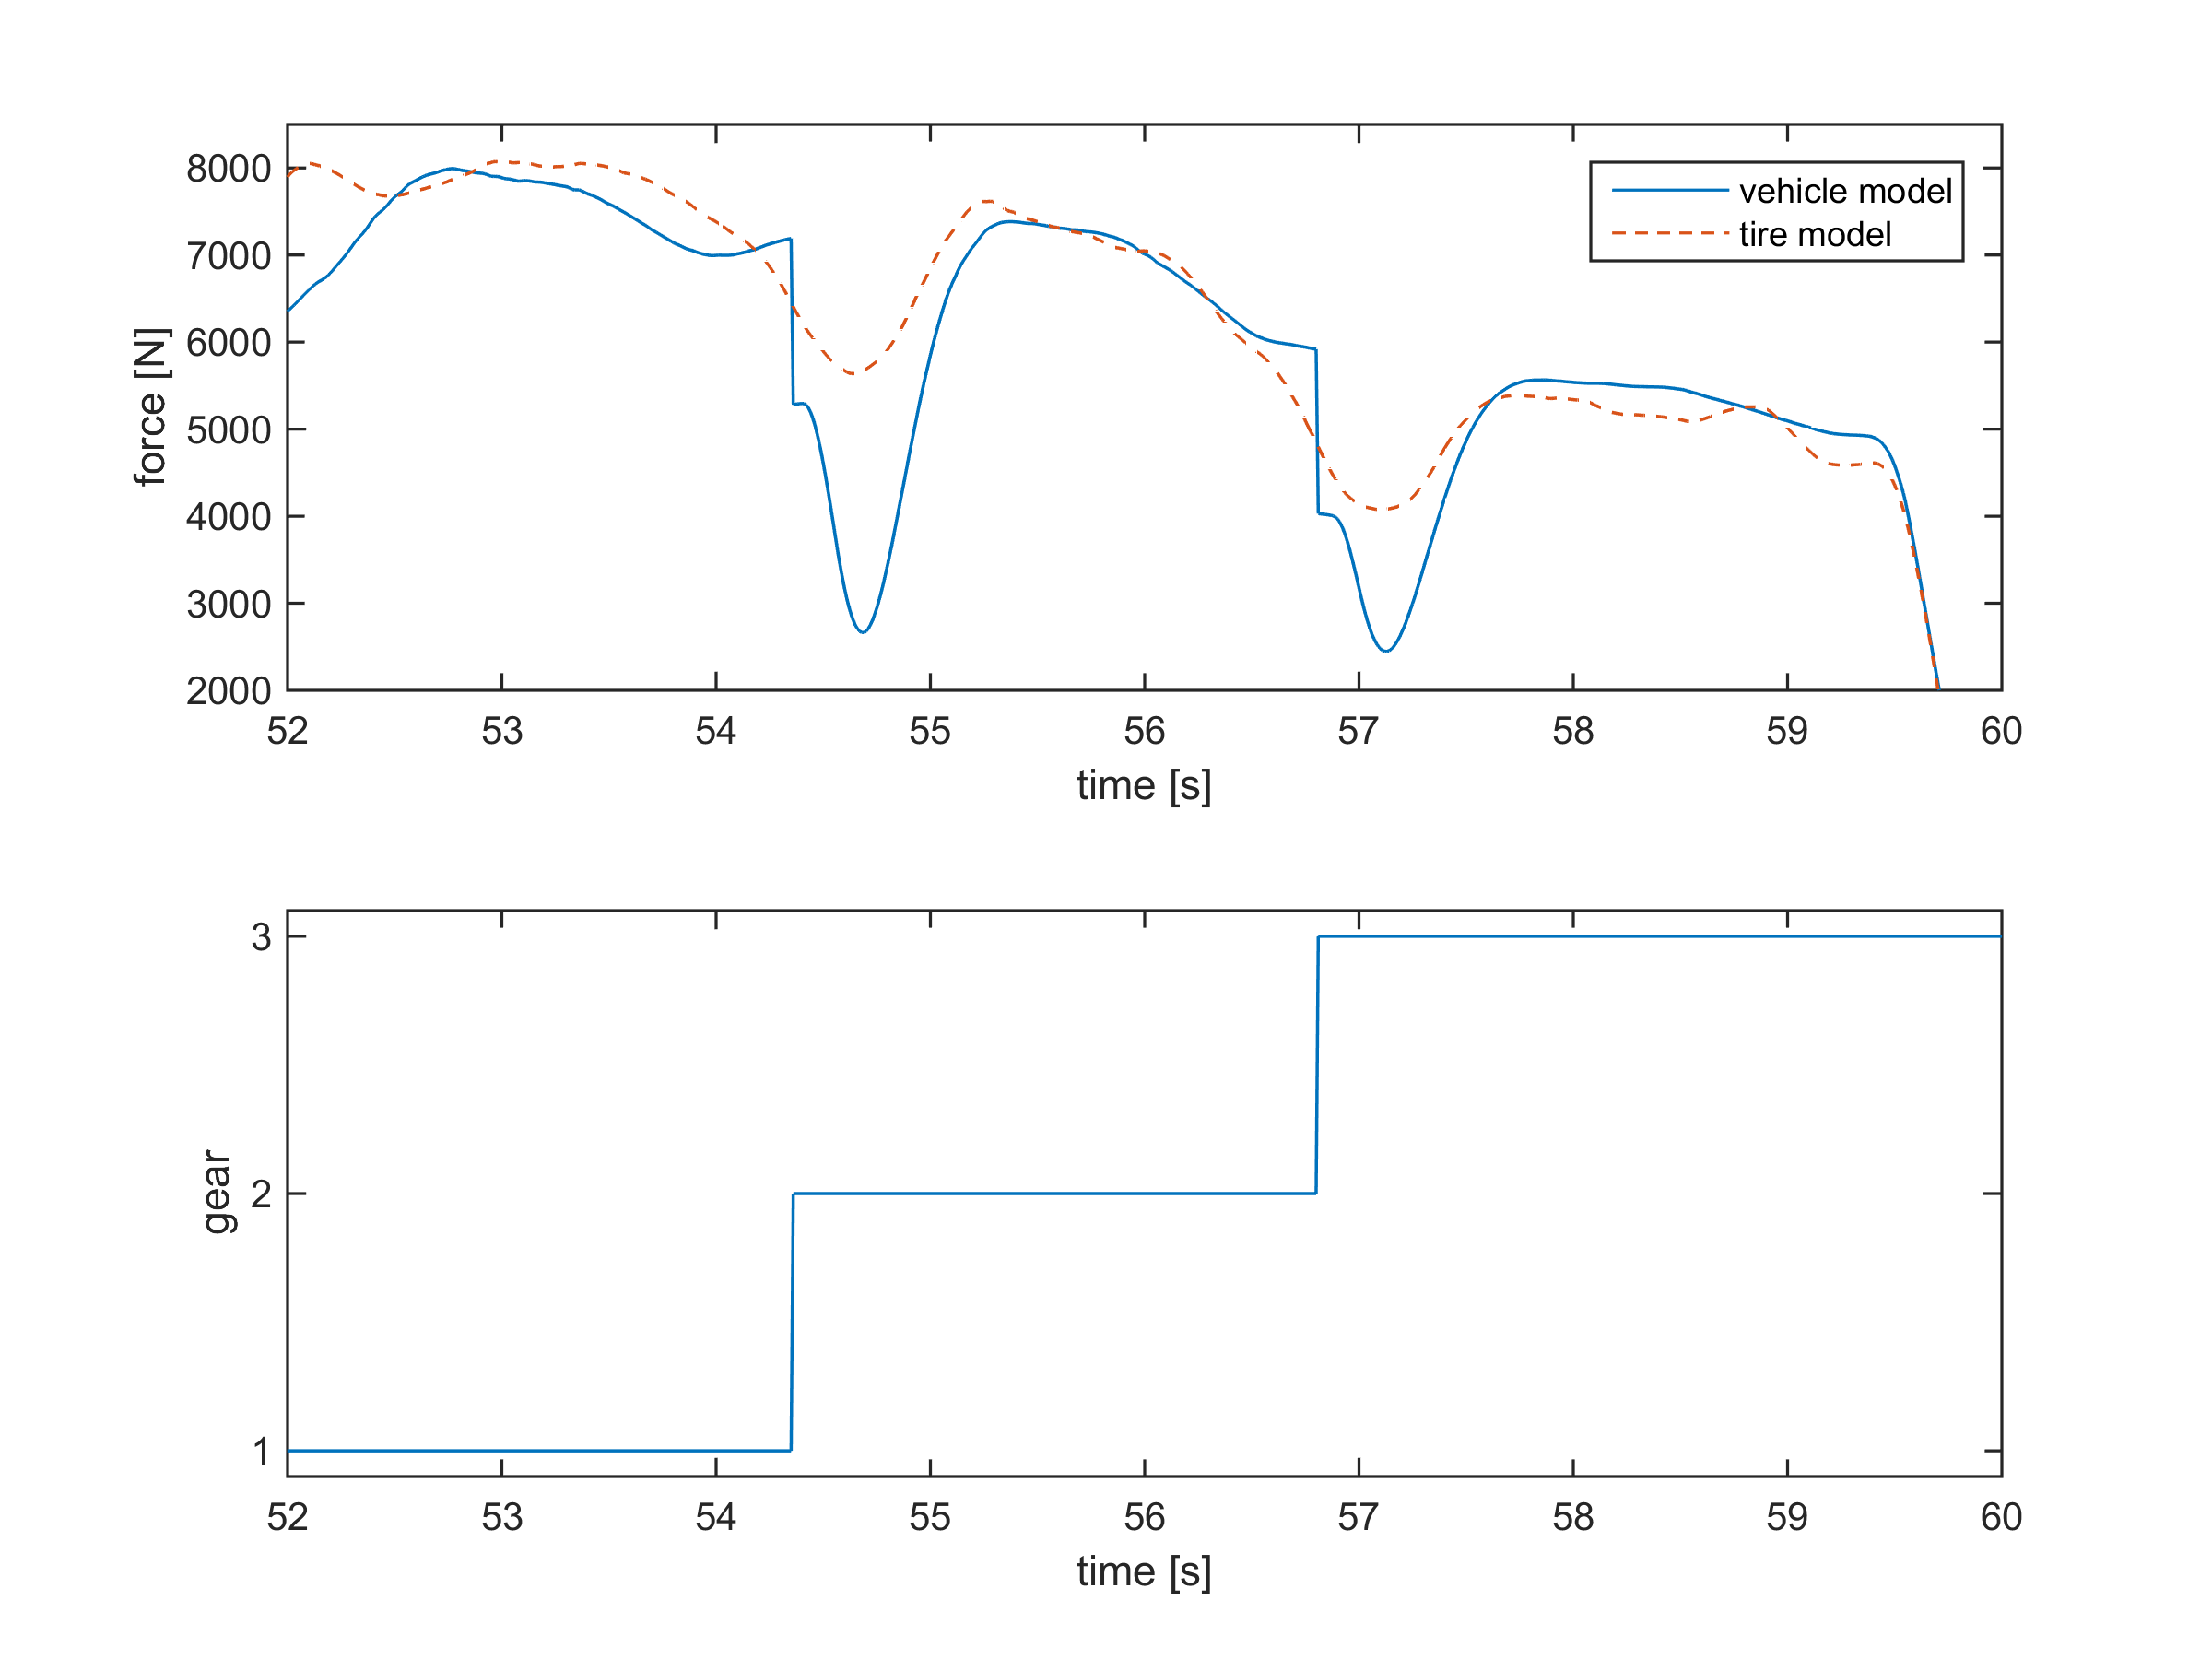
\includegraphics[width=1.0\textwidth]{Pictures/gear_change}
	\caption {Vehicle and tire forces when changing gear.}
	\label{gear_change}
\end{figure}

Due to this disturbance during the gear change, the RLS fitting method should not be updated during a certain amount of time after a gear change occurs. A new friction coefficient can therefore not be calculated during this period. 

\subsubsection{Limitations due to low forces}
Another limitation that adds to the restrictions when the friction coefficient shouldn't be updated is when the total forces acting on the vehicle is too low. During this period of time, when the normalized force is far from the friction coefficient limit, it is very hard to approximate the actual value of the friction coefficient. The reason to this is that the force from the tire model changes less when low forces acting. This can also be seen in Figure \ref{different_mue} in Section \ref{section_friction coefficient}. It can be seen that amount of force generated for a certain friction coefficient varies very little for the lower slip ratio values. Small errors between the forces from the models will therefore generate a larger change of the friction coefficient which is undesired. 

The RLS should, due to the reasoning above, not be updated when the normalized forces from both the vehicle and tire model is a certain amount below the friction coefficient. This means that the friction coefficient will be updated rarely during calmer driving sequences, which becomes a trade-off to getting a more stable friction coefficient estimator. 

\section{Other methods}

\subsection{Slip-slope friction model}

One friction model that is frequently used and referred to in research papers is the so called slip-slope friction model. The models general idea is that the maximum tire/road friction available can be decided due to its dependency on the slope from the slip-force curve in the linear region. This slip-force curve has the same characteristics as the slip-friction coefficient curve seen in Figure \ref{fric_slip}. 
\begin{equation}
\dfrac{F_{x}}{F_{z}} = k \cdot \kappa
\end{equation}
Where $ F_{x} $ and $ F_{z} $ is the estimated longitudinal and normal force acting on a tire depending on input values. The slip-slope can be estimated with for example recursive least square fitting.
 % Experiment 1

%\chapter{Results}
\label{chapter_five}

\section{Tire/road friction for different driving sessions}
The most interesting result of all this work is of course the estimated tire/road friction coefficient. But, how the estimator works with the forces and when it actually estimates the friction is also interesting. Most of the resulting plots consist of two subplots, the estimated friction but also the vehicle force and the tire force. The vehicle force is always calculated but the tire force is only estimated in accordance with Section \ref{when_to_estimate}. When these conditions aren't fulfilled the tire force is set to zero in the plots and the estimator is paused.

To eliminate minor disturbances the combined forces for the two front tires are used rather than splitting it up into two different computations. This means that only one friction coefficient will be estimate rather than one for each tire respectively. It would be possible to calculate the friction coefficient for both sides of the vehicle in order to detect a split-$ \mu $ situation, but the trade off would be a less stable estimation when both tires have the same friction to the road. A more stable estimation is prioritized in this report.

\subsection{Winter tires on asphalt}
The algorithm that estimate the friction coefficient was run on the straight line acceleration run, as used in Section \ref{winter_tire} to acquire the tire model parameters. The combined forces from the two front tires can be seen for the two respective force models in Figure \ref{force_mue_olika_acc}, subplot one. The corresponding friction coefficient can be seen in subplot two. 

\begin{figure}[h]
	\centering
	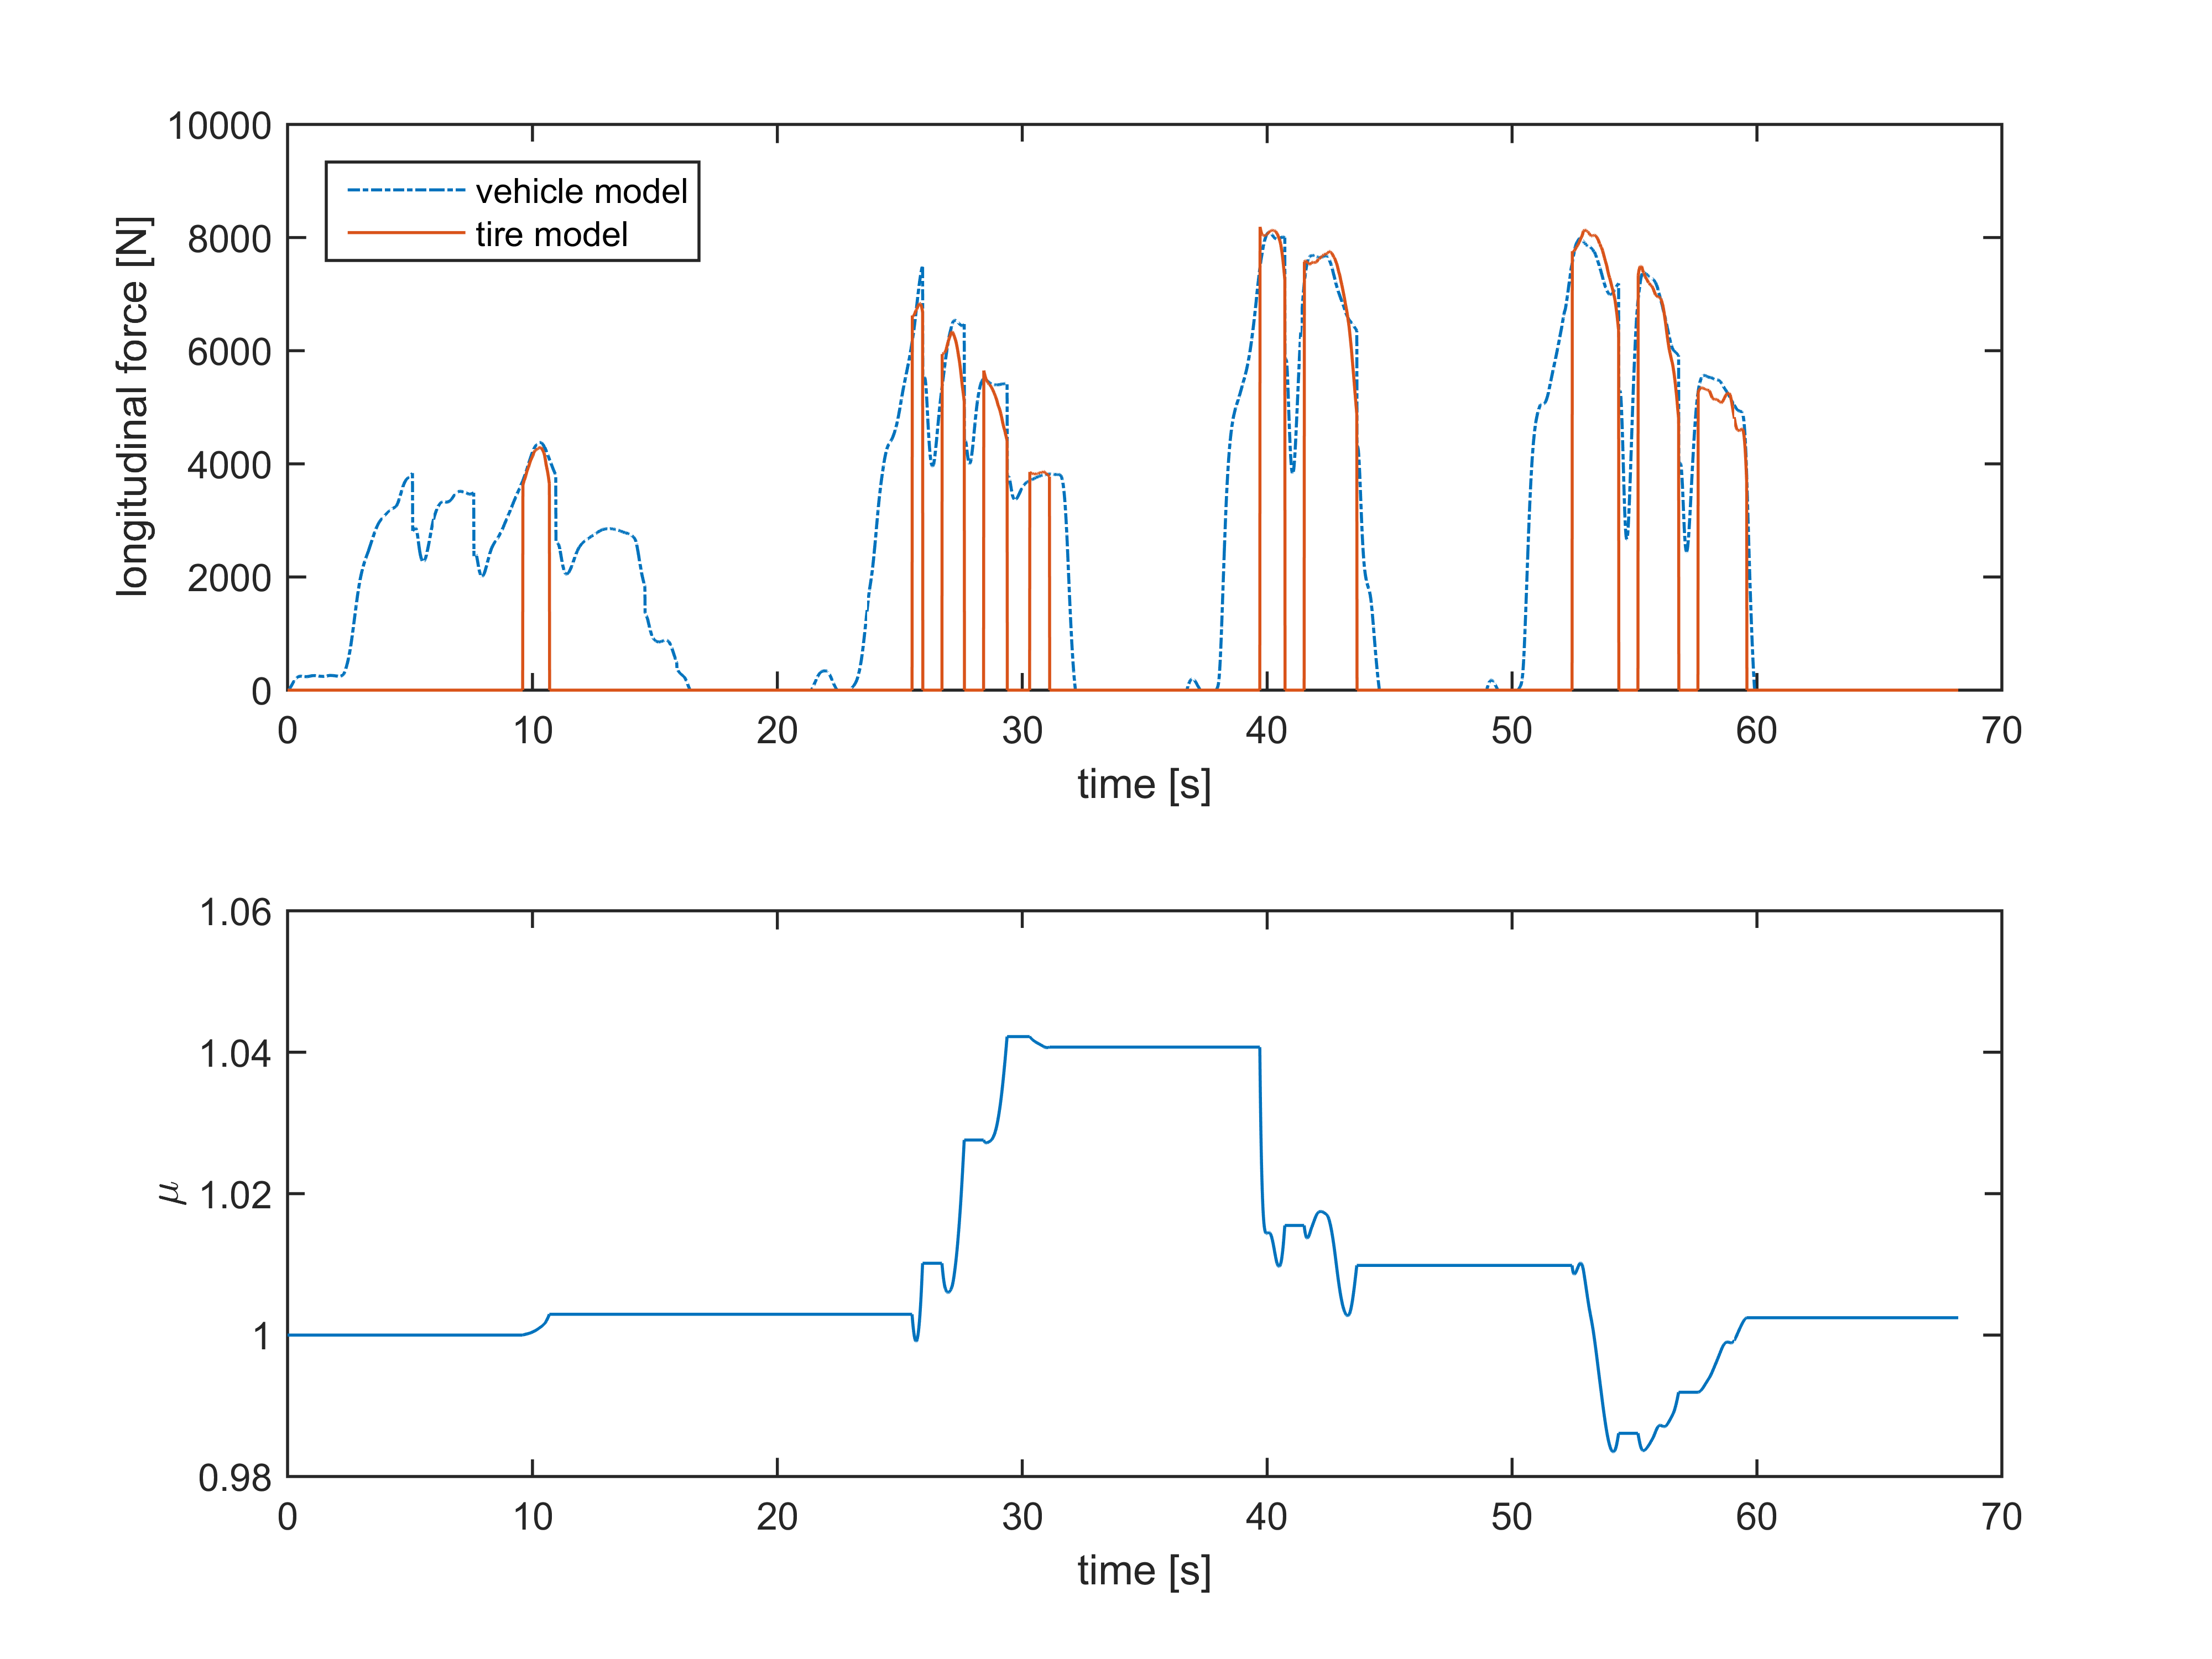
\includegraphics[width=1.0\textwidth]{Pictures/force_mue_olika_acc}
	\caption {Force from the tire and vehicle model and the estimated $ \mu $ for a straight line acceleration.}
	\label{force_mue_olika_acc}
\end{figure}

The friction estimation is seen to be jumpy at certain times, but the changes of frictional value are still quite small. The friction estimation stays around $ \mu = 1 $, which it evidently should due to the fact that the tire model parameters are fitted during this driving sequence. 

A more interesting test for the friction estimation algorithm is a driving sequence done as the fast track run. The same tires were used on a similar surface as in the previous driving sequence. The force from the two models and the friction estimation result can be see in Figure \ref{force_mue_race}. 

\begin{figure}[h]
	\centering
	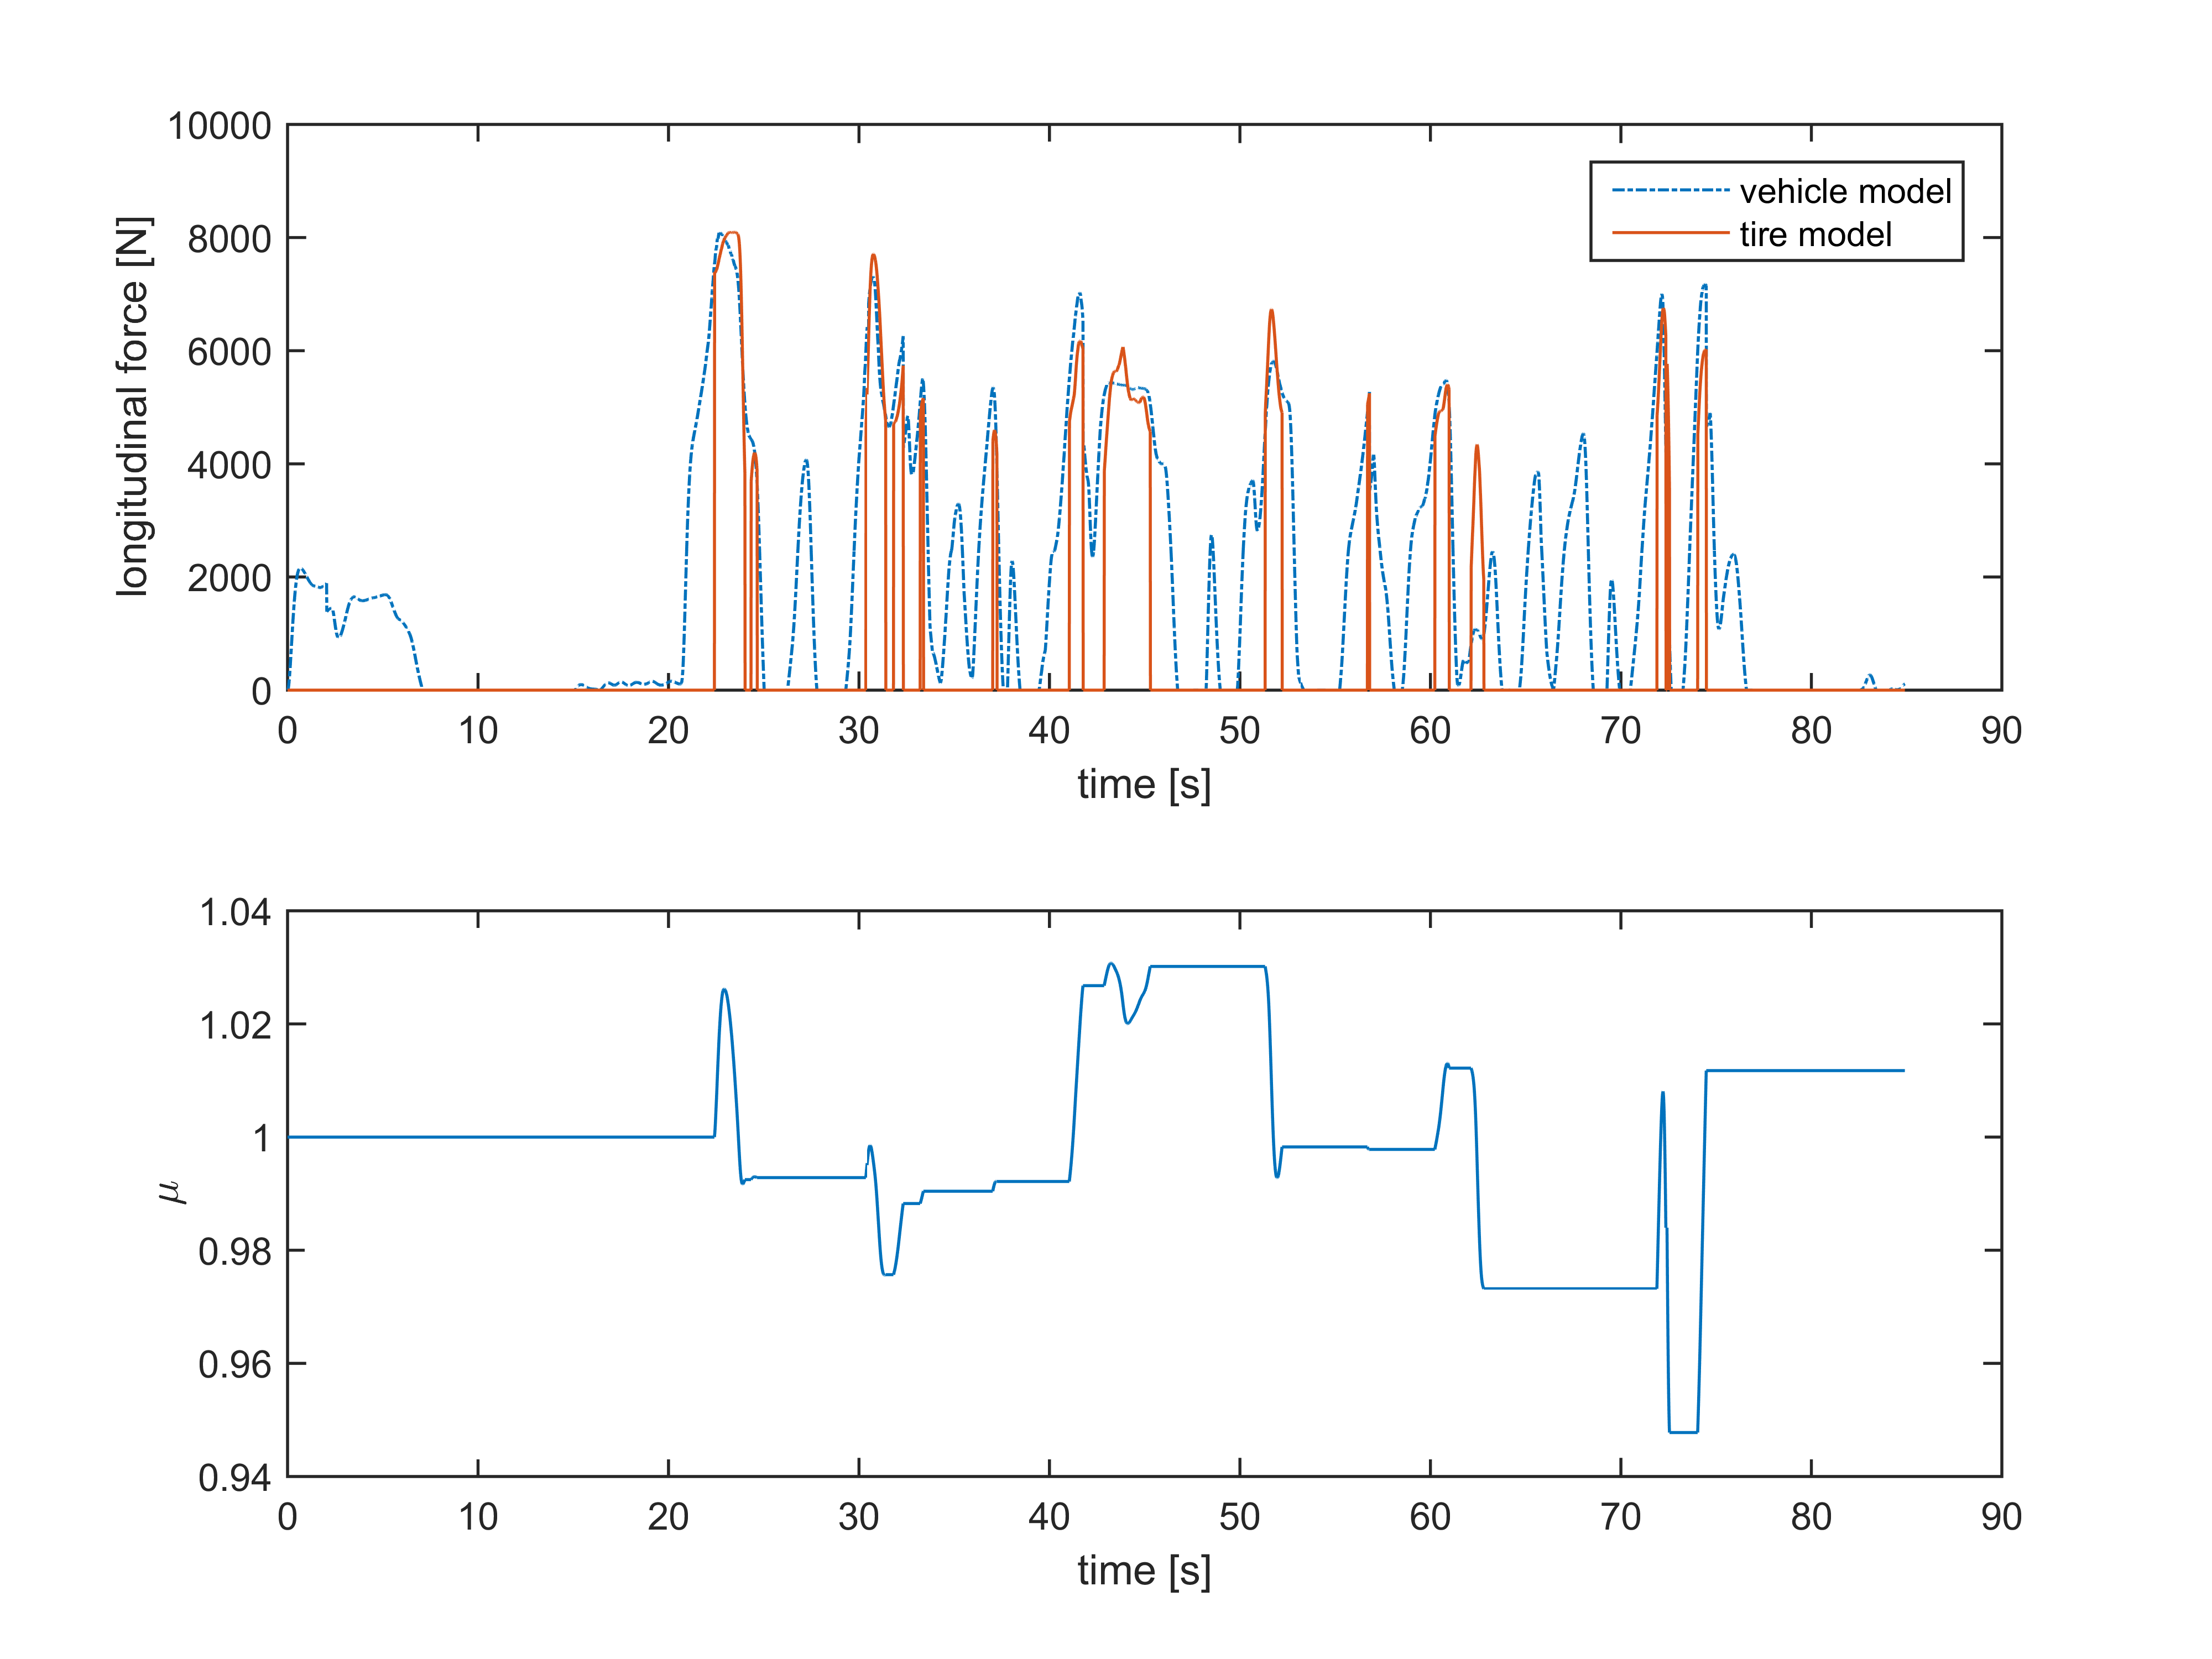
\includegraphics[width=1.0\textwidth]{Pictures/force_mue_race}
	\caption {Force from the tire and vehicle model and the estimated $ \mu $ for a fast track run.}
	\label{force_mue_race}
\end{figure}

The resulting friction coefficient is seen to vary around $ \mu = 1 $, similar to the straight line acceleration run. In the first subplot, it can be seen that the force from the tire model is calculated quite rarely, meaning that the friction coefficient is only estimated during these moment. However, the resulting $ \mu $ estimated during these moments are fairly steady around $ \mu = 1 $. 

\subsection{Winter tires on ice}
Being able to detect a surface with a low friction coefficient is probably the most important part of the friction estimation algorithm, due to the risk of an accident if too much torque is transferred to one of the driving axles. The resulting forces from the models and the estimated friction coefficient can be seen for a driving sequence on ice/snow in Figure \ref{force_mue_ice_normal}.

\begin{figure}[h]
	\centering
	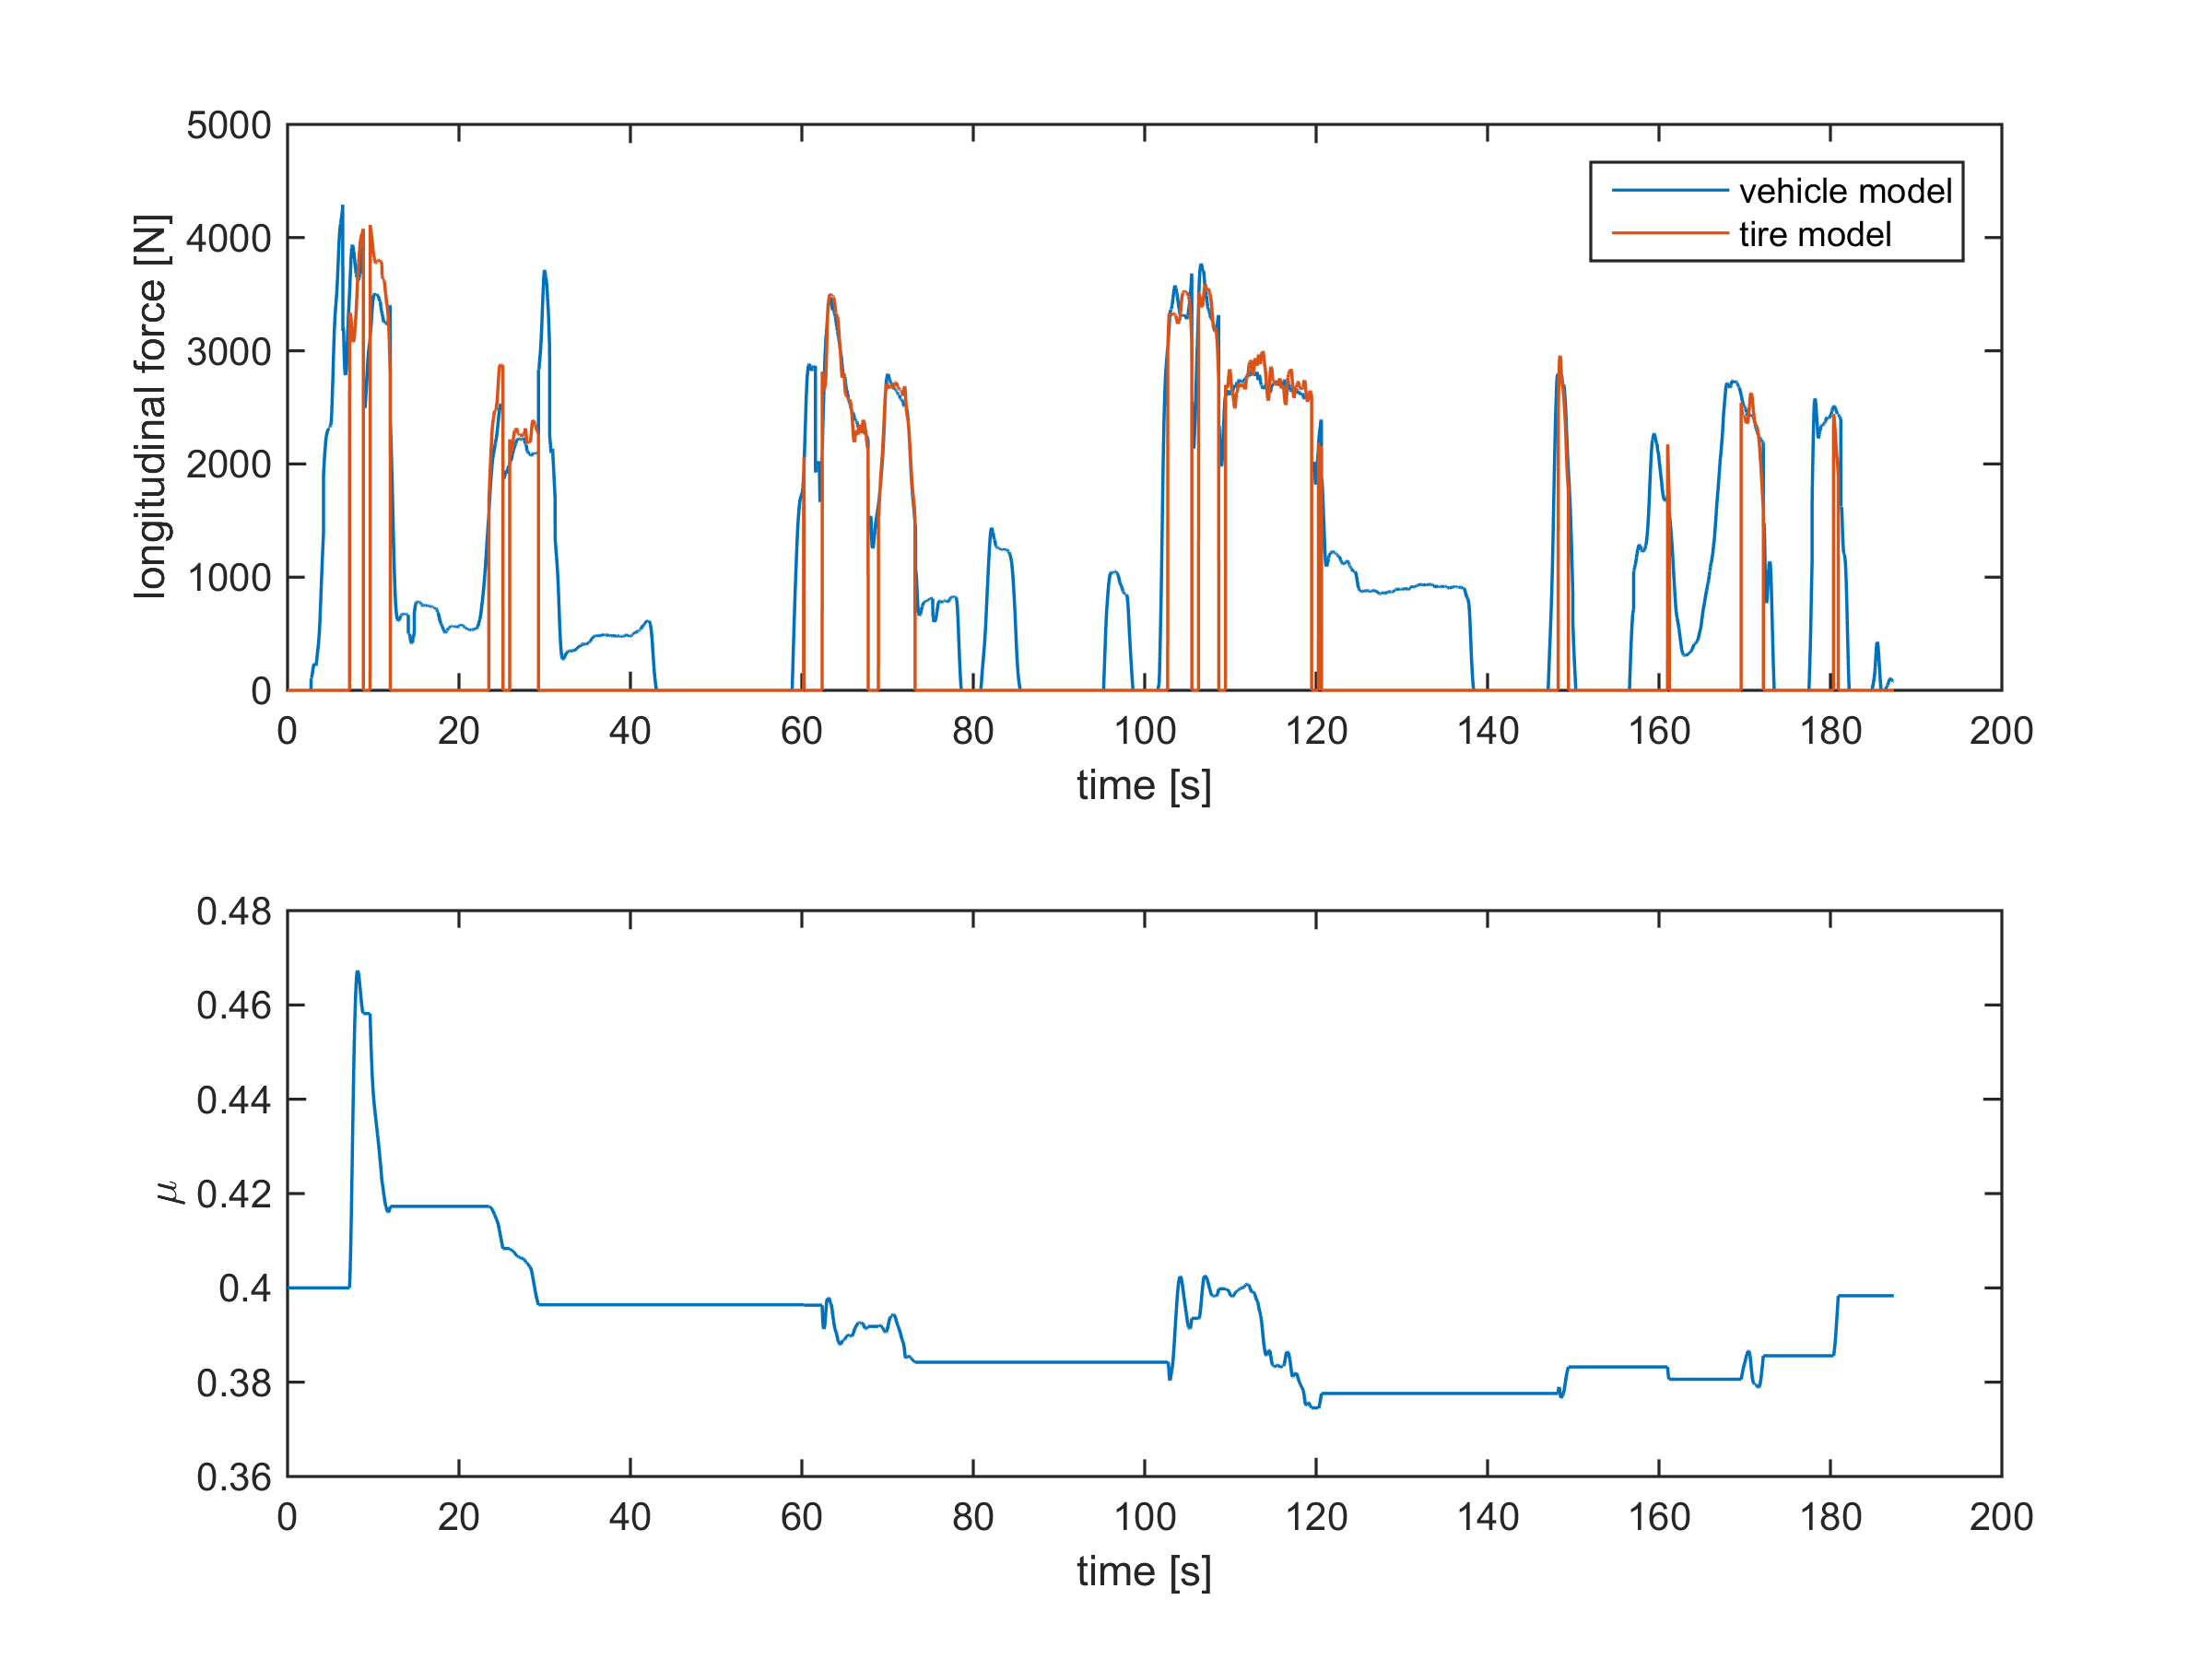
\includegraphics[width=1.0\textwidth]{Pictures/force_mue_ice_normal}
	\caption {Force from the tire and vehicle model and the estimated $ \mu $ for a driving sequence on ice/snow.}
	\label{force_mue_ice_normal}
\end{figure}

The winter tire model parameter for low-$ \mu $ was fitted on this run. It is therefore no coincidence that the friction coefficient end up at around $ \mu = 0.4 $. It can be seen in the figure that the force calculated from the tire model varies with a higher frequency during the driving sequence on ice/snow compared to the previous sequences. Even though, the resulting friction coefficient is estimated fairly well around friction $ \mu = 0.4 $, especially when the estimation algorithm is active for a relatively large period of time seen at $ \approx 100-120 $ s. A quite large disturbance of $ \mu $ can unfortunately be seen at the times $ \approx 7 - 12$ s, due to that the vehicle model calculates a higher force than the tire model.  

\subsection{Winter tires on asphalt and ice combined}
The main goal for the work done in this report was to detect when low-$ \mu $ is present so that the torque transfer through the FXD can be limited. It is therefore essential to test the developed algorithm during a driving sequence that actually includes a change of $ \mu $, preferably from high-$ \mu $ to low-$ \mu $, to verify that the algorithm can handle this kind of abrupt change. It has not been possible to test this on a single run, for example using a driving sequence that includes both asphalt as well as a skid pad. In order to simulate this behavior, two different runs have been merged together, where the friction coefficient changes a total of three times. Starting at high-$ \mu $ and finishing with low-$ \mu $. The merging was made at points where both sequences were accelerating or decelerates at the same velocity, in order to avoid unnecessary jumps of other signals from the vehicle. 

The two modeled forces and the resulting $ \mu $ from the merged run can be seen in Figure \ref{force_mue_comb2}. The estimated friction coefficient is seen to clearly change when a different driving sequences is begun, meaning that the algorithm manages to detect that the grip between the tire and the road differs.
 
\begin{figure}[h]
	\centering
	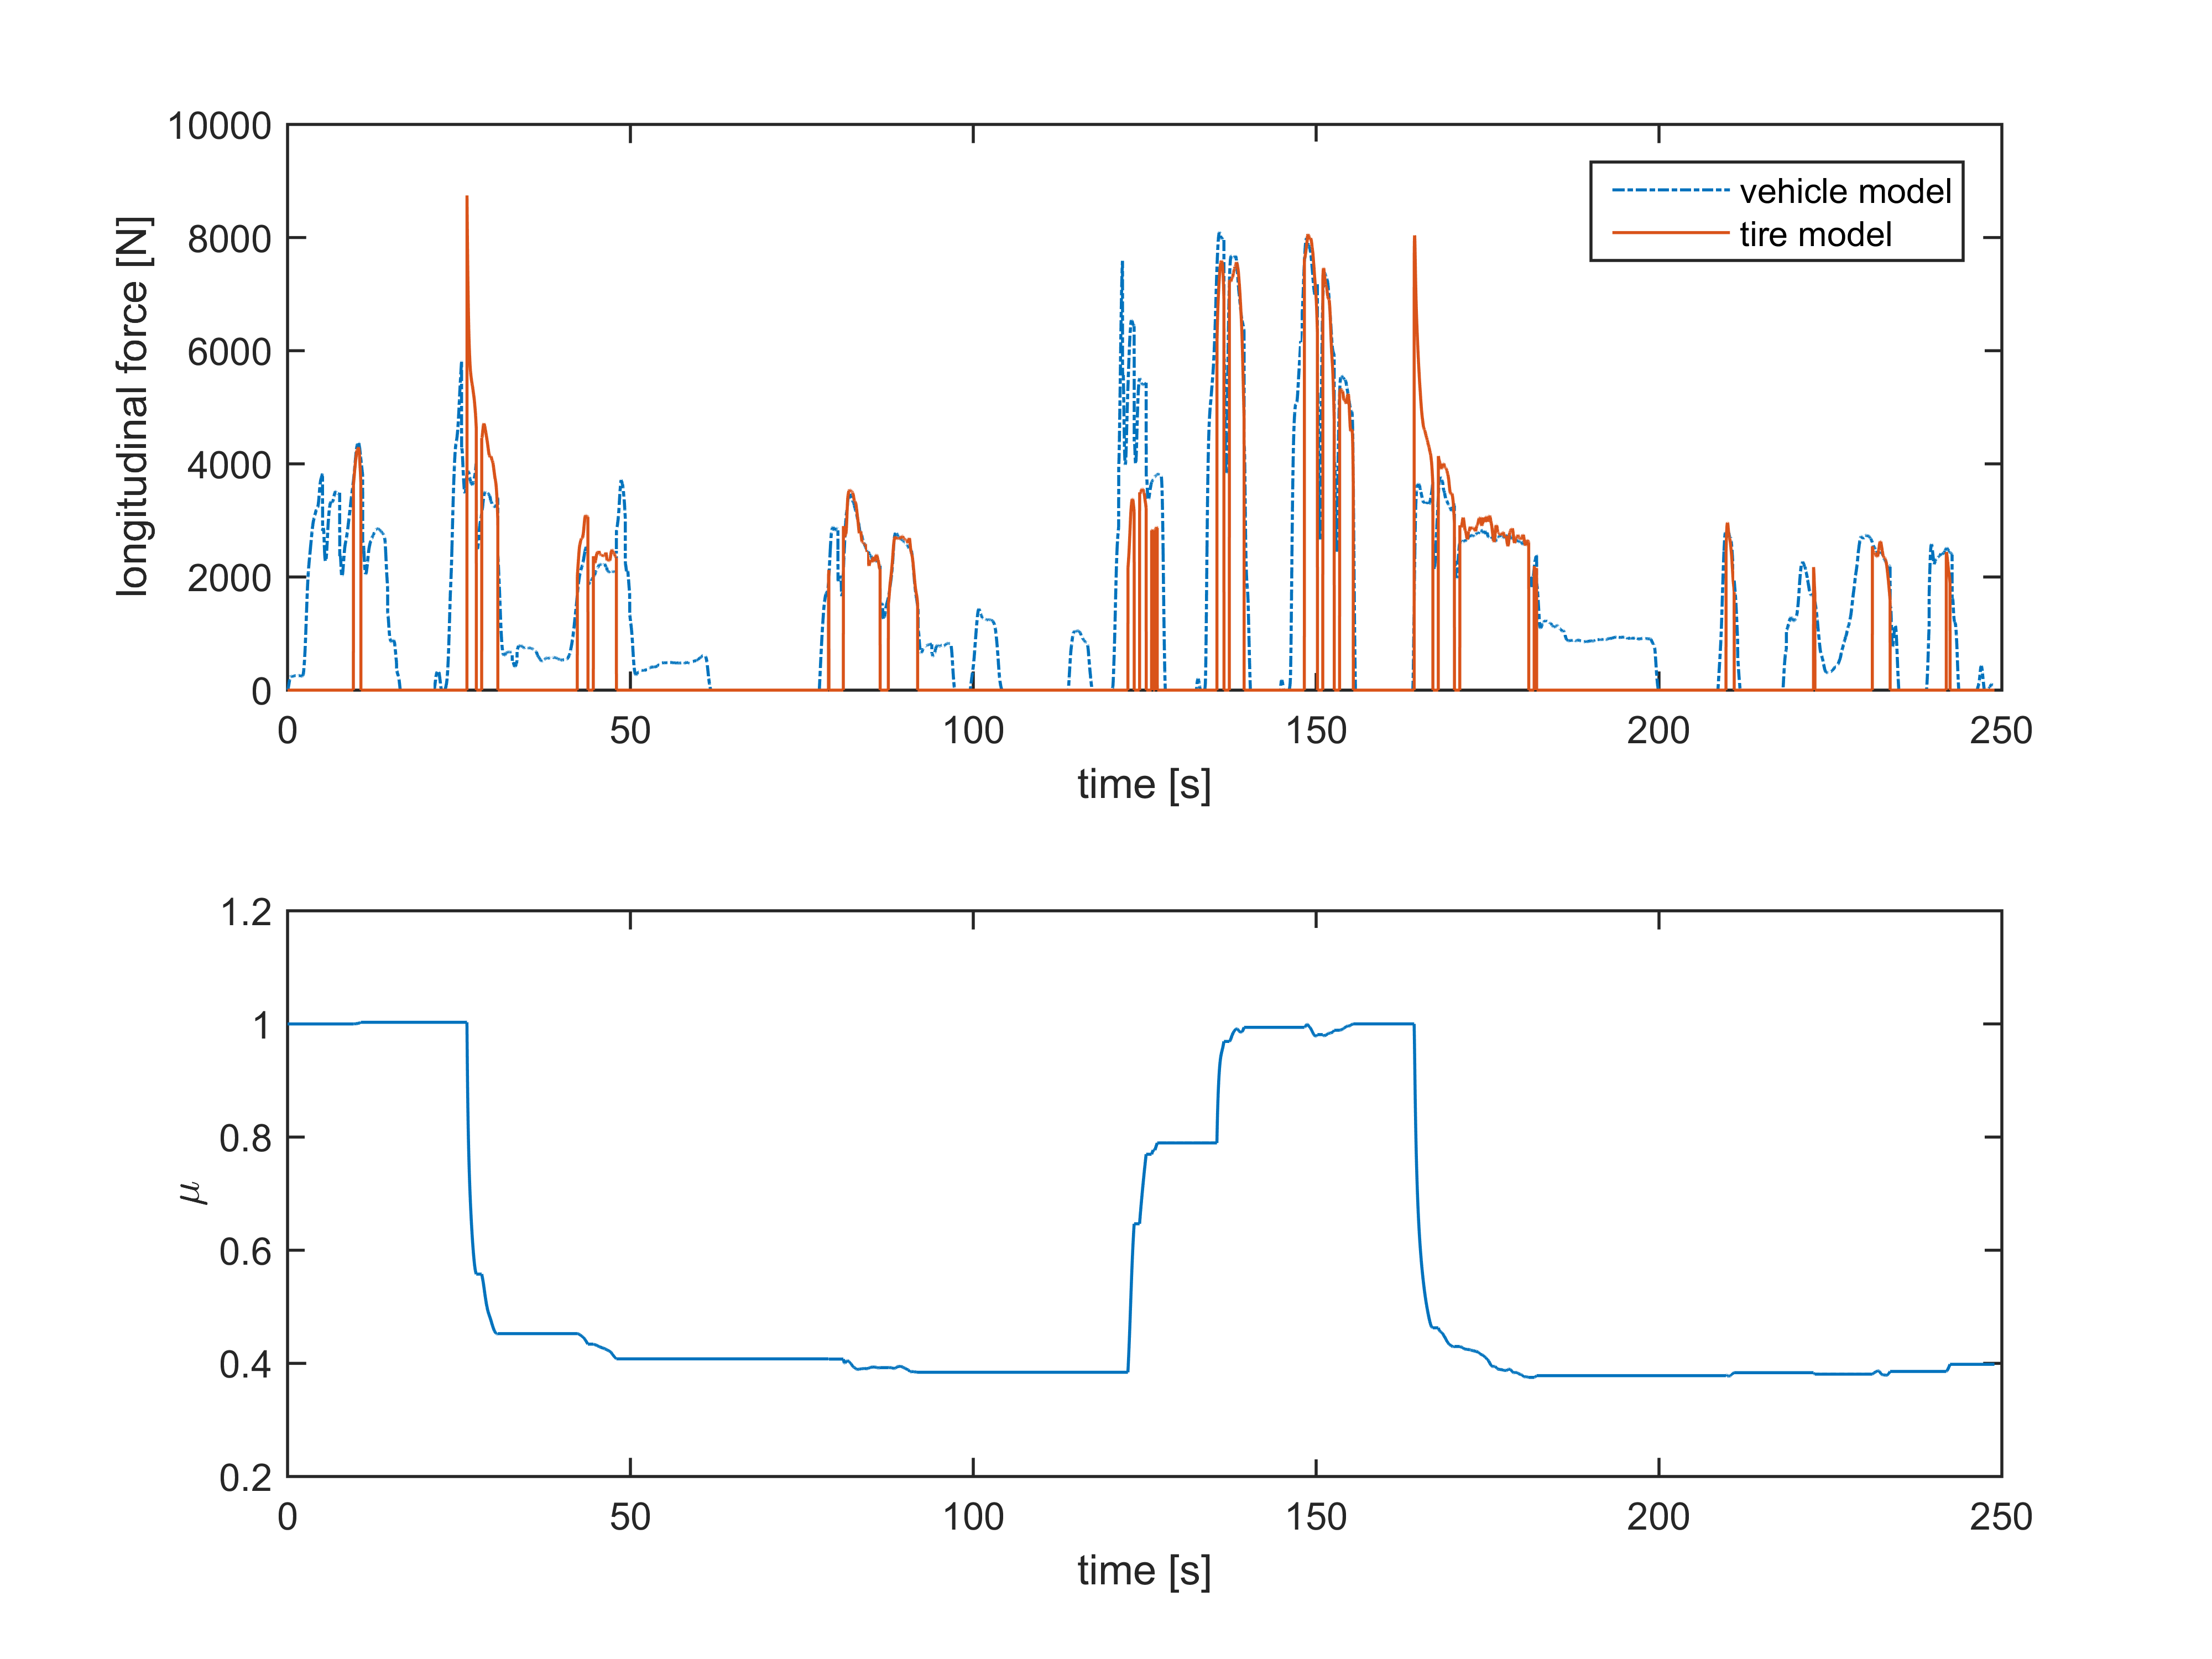
\includegraphics[width=1.0\textwidth]{Pictures/force_mue_comb2}
	\caption {Force from the tire and vehicle model and the estimated $ \mu $ for two different runs with differing $ \mu $ merged together.}
	\label{force_mue_comb2}
\end{figure}

Due to the limitations set concerning when the friction coefficient should be estimated (Section \ref{when_to_estimate}), the algorithm may not update $ \mu $ at the same instance as the new surface is present. However, when the algorithm is allowed to estimate, the new friction coefficient is estimated with good speed. In Figure \ref{force_mue_comb2_zoom}, the two forces and the friction coefficient can be seen when the result is zoomed in on a sudden drop of the friction coefficient. The converging $ \mu $ is seen to drop very fast as the two forces differs greatly right after $ \approx 26.2 $ s, and thereafter decrease more slowly. 

\begin{figure}[!]
	\centering
	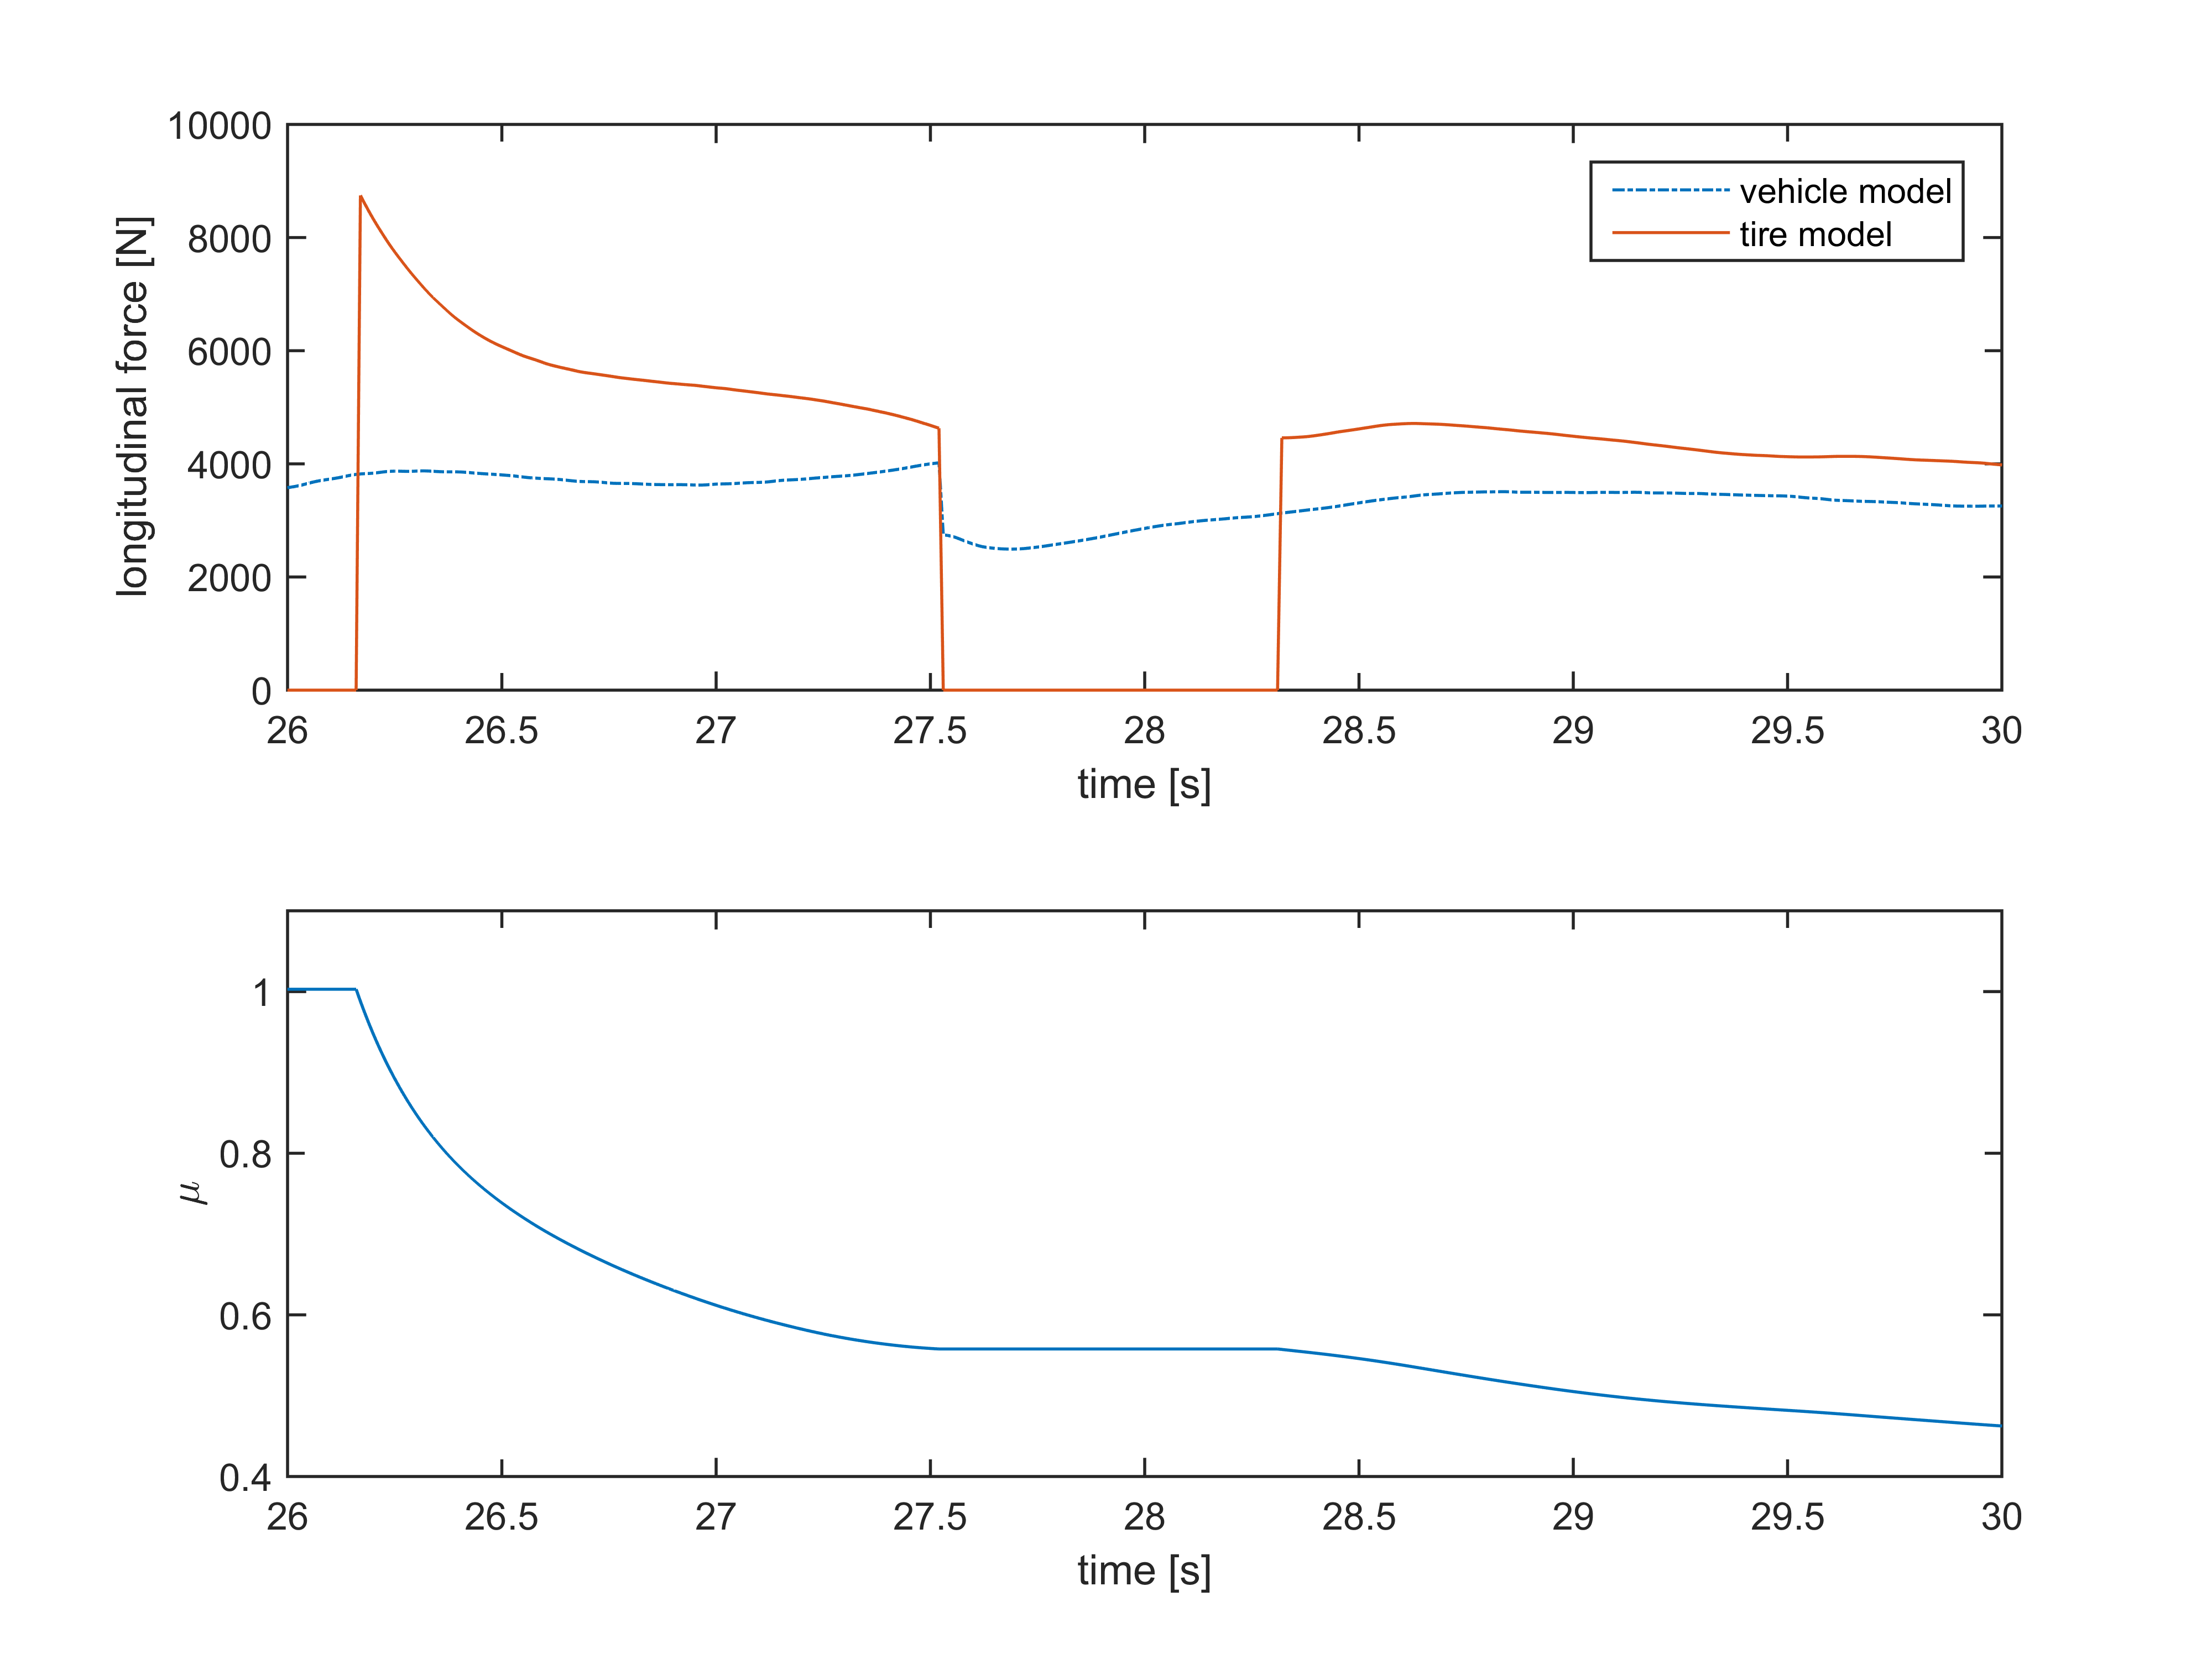
\includegraphics[width=0.95\textwidth]{Pictures/force_mue_comb2_zoom}
	\caption {Zoomed in result of Figure \ref{force_mue_comb2}, showing the speed of the friction coefficient algorithm.}
	\label{force_mue_comb2_zoom}
\end{figure}

The normalized force per slip ratio curve for the combined sequence can be seen in Figure \ref{slip_kraft_comb2}. Note that this figure is merely the two Figures \ref{slip_kraft_ljungby} \& \ref{slip_kraft_is} added on top of each other, with some erroneous result due to the wrong calculated force when the friction coefficient suddenly changes. The result clearly shows that a tire's stiffness varies for surfaces.

\begin{figure}[!]
	\centering
	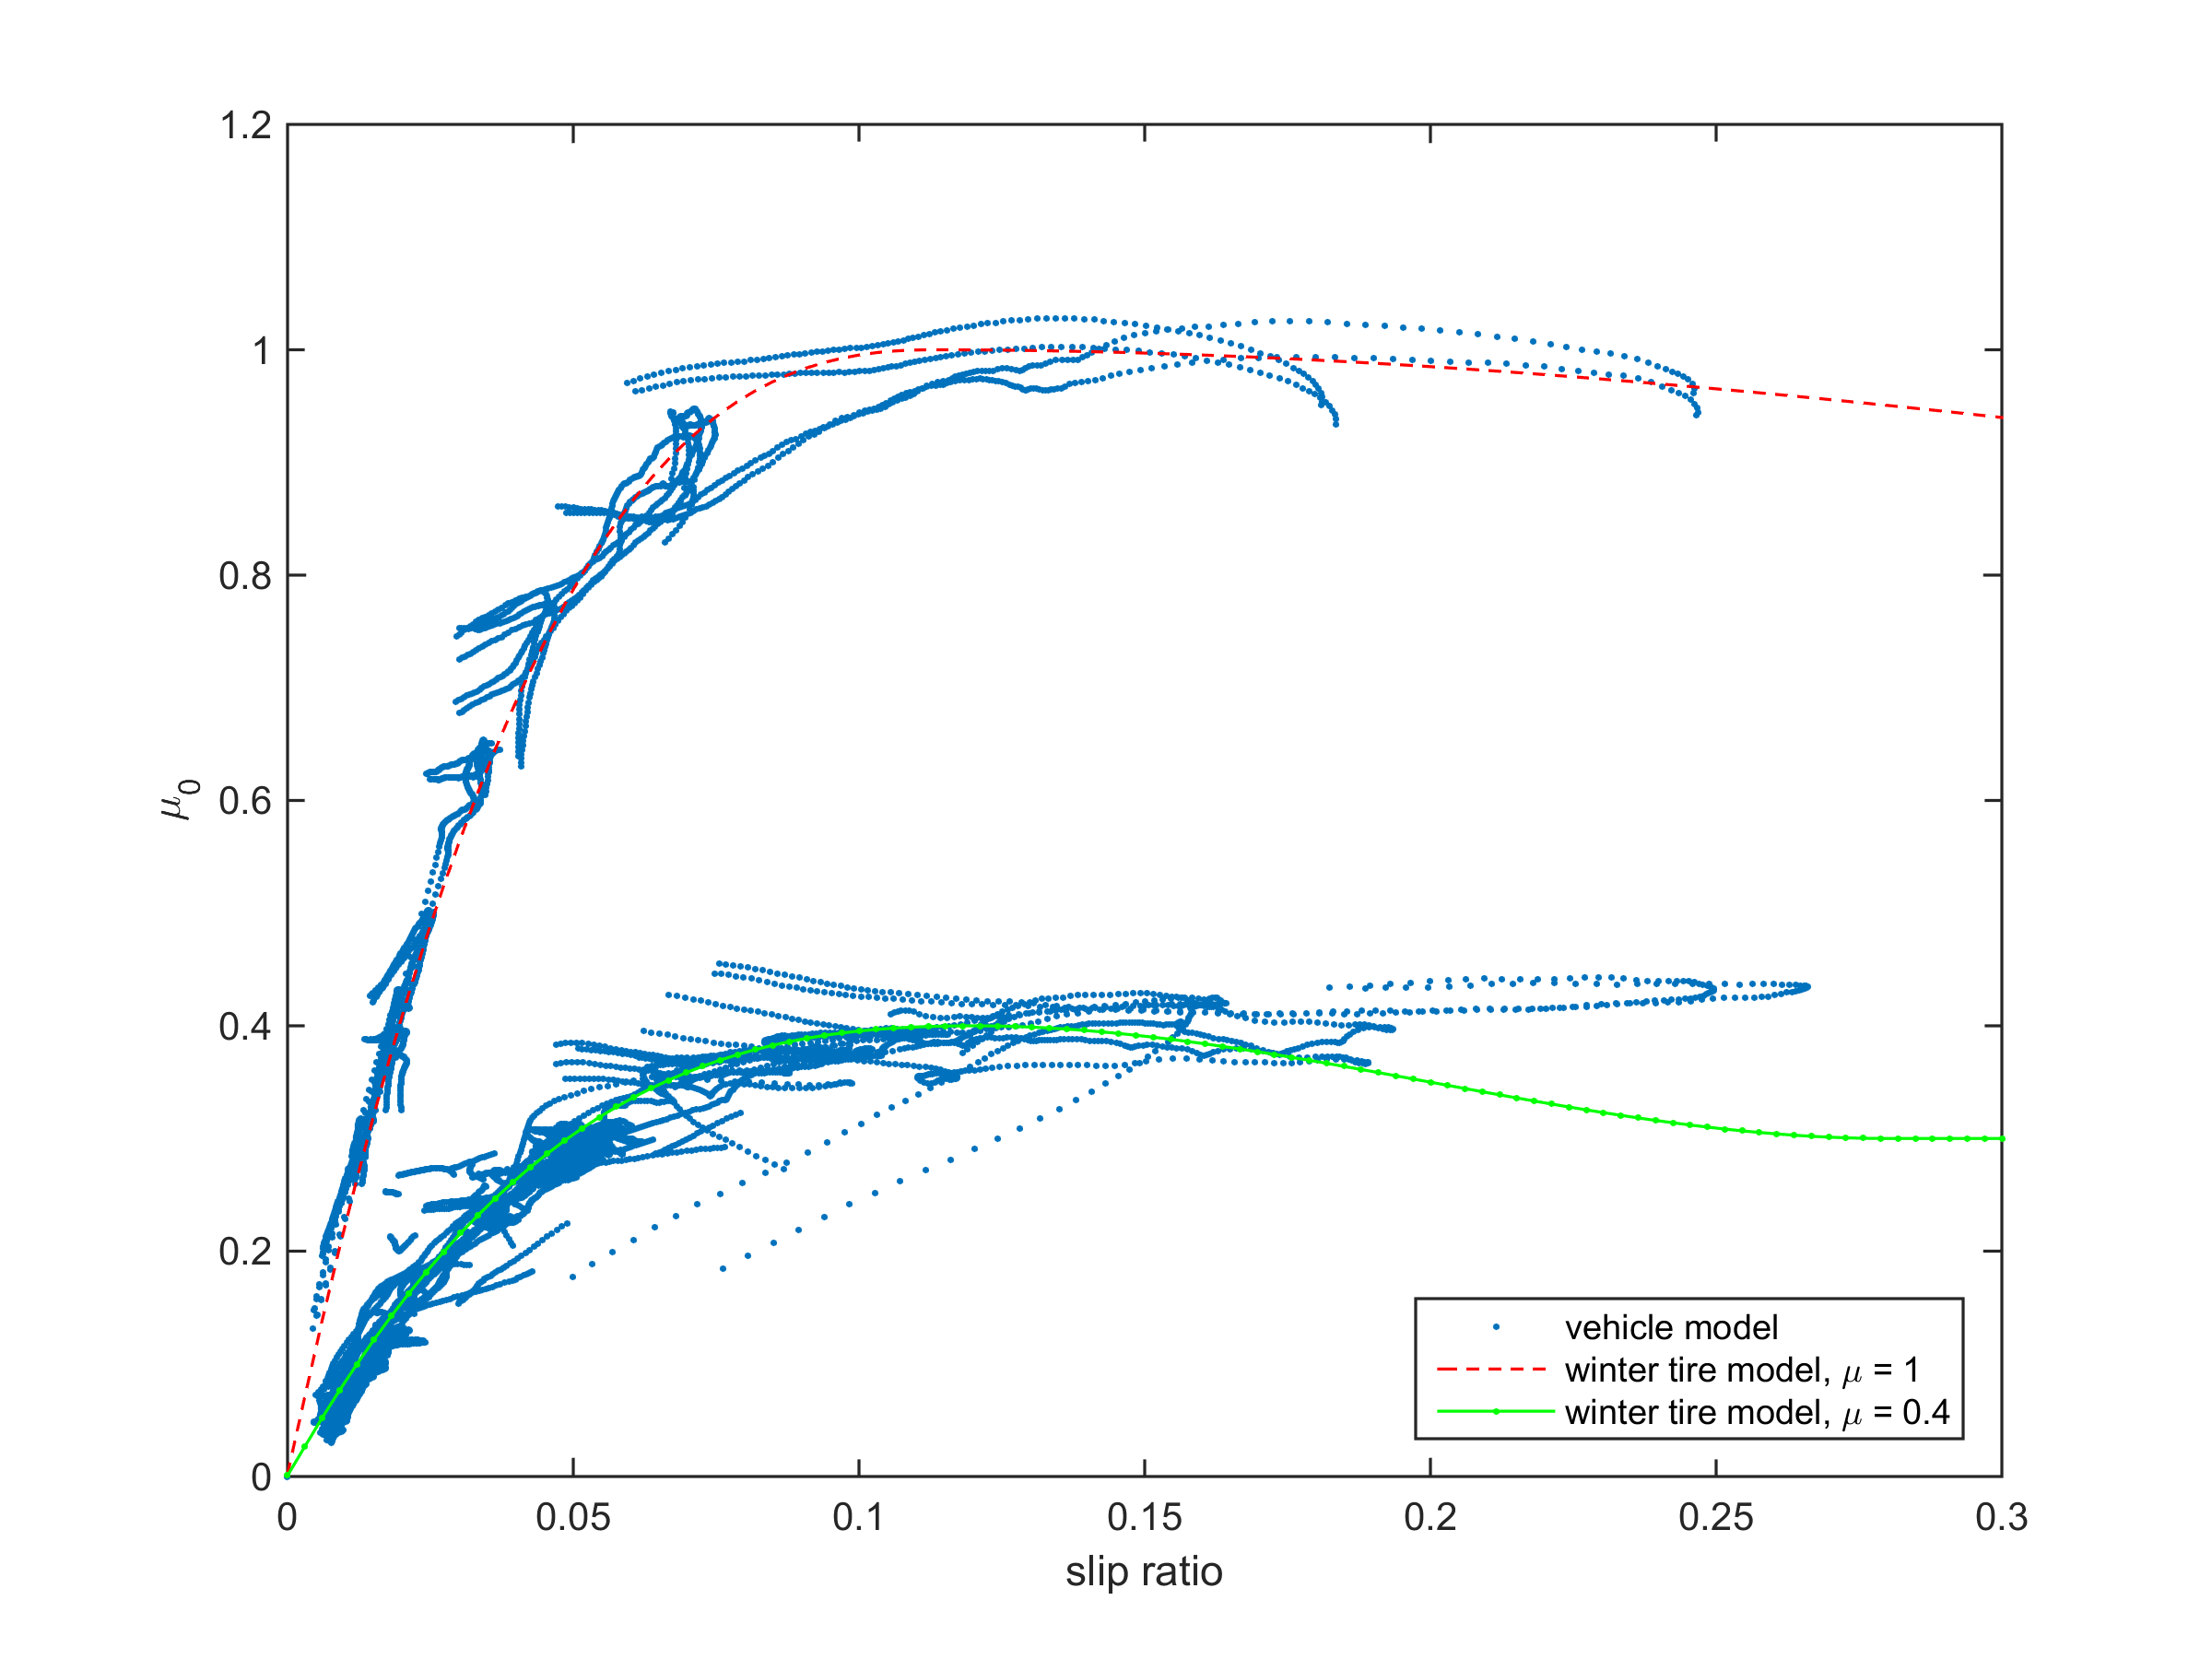
\includegraphics[width=0.95\textwidth]{Pictures/slip_kraft_comb2}
	\caption {Force per slip ratio for the combined driving sequence with both low- and high-$ \mu $.}
	\label{slip_kraft_comb2}
\end{figure}

\pagebreak
\subsection{Summer tires on asphalt}
A fast track lap was also run with the summer tires on asphalt. These tires were, as mentioned before, relatively stiff and with the peak force located at a relative small slip ratio value. This tire attribute makes it tougher to estimate the friction coefficient, due to the fact that variances will result in larger force errors between the two models.

The result from this fast track run can be seen in Figure \ref{force_mue_race_bb}. The two first curves, \textit{vehicle model} and \textit{tire model, used value}, are the same calculations as seen earlier in the result, and \textit{tire model, all values} is an additional plot that shows the tire force even when the conditions are not met from Section \ref{when_to_estimate}. The conditions are unfortunately not met at any longer period of times, as the figure shows, even though the forces acting on the vehicle are relatively high at numerous occasions. Hence the curve \textit{tire model, all value} is shown to demonstrate the reasons that the conditions for the friction estimation algorithm are not met.

\begin{figure}[h]
	\centering
	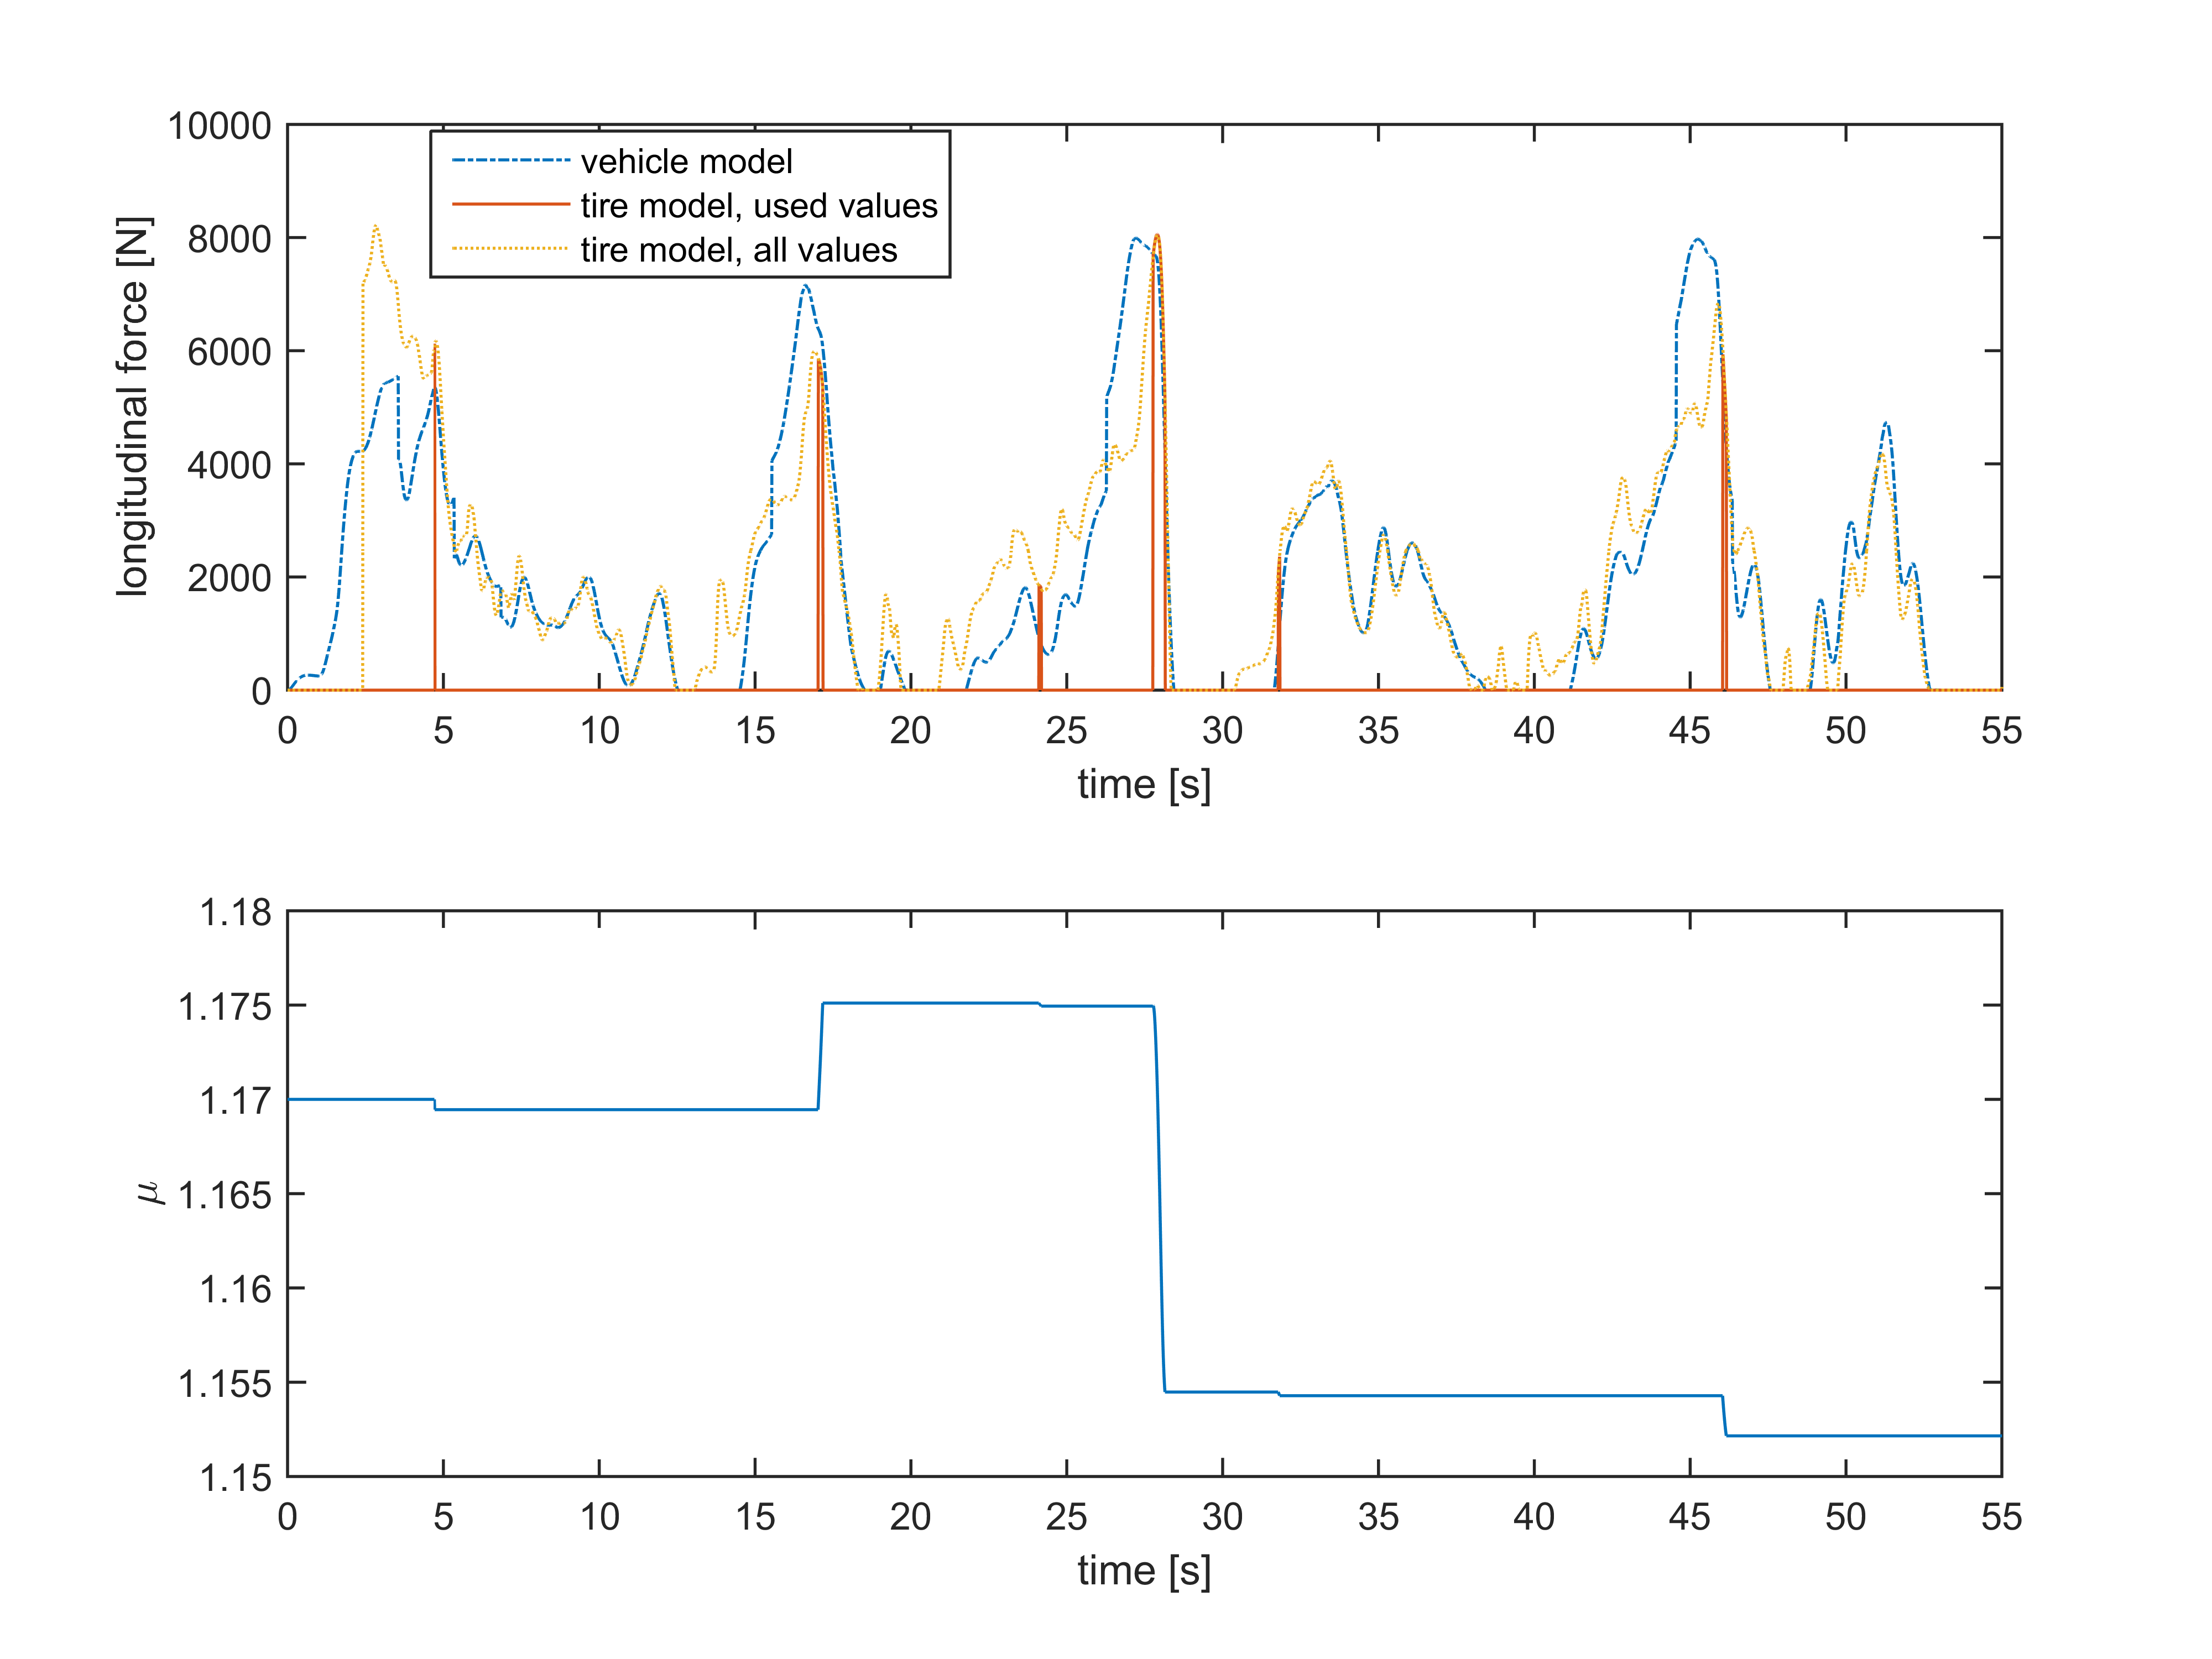
\includegraphics[width=1.0\textwidth]{Pictures/force_mue_race_bb}
	\caption {Force from the tire and vehicle model and the estimated $ \mu $ for a driving sequence on dry asphalt with summer tires.}
	\label{force_mue_race_bb}
\end{figure}

\subsection{Summer tires on wet asphalt}
A similar fast track lap was done with the summer tires on wet asphalt, to test the algorithm's behavior on the similar road surface but with different driving conditions. The result from this driving sequence can be seen in Figure \ref{force_mue_blot_race_bb}. It can be seen that the resulting $ \mu $ does not drop much lower than the $ \mu = 1.17 $ which was calculated during the dry acceleration run. 

\begin{figure}[h]
	\centering
	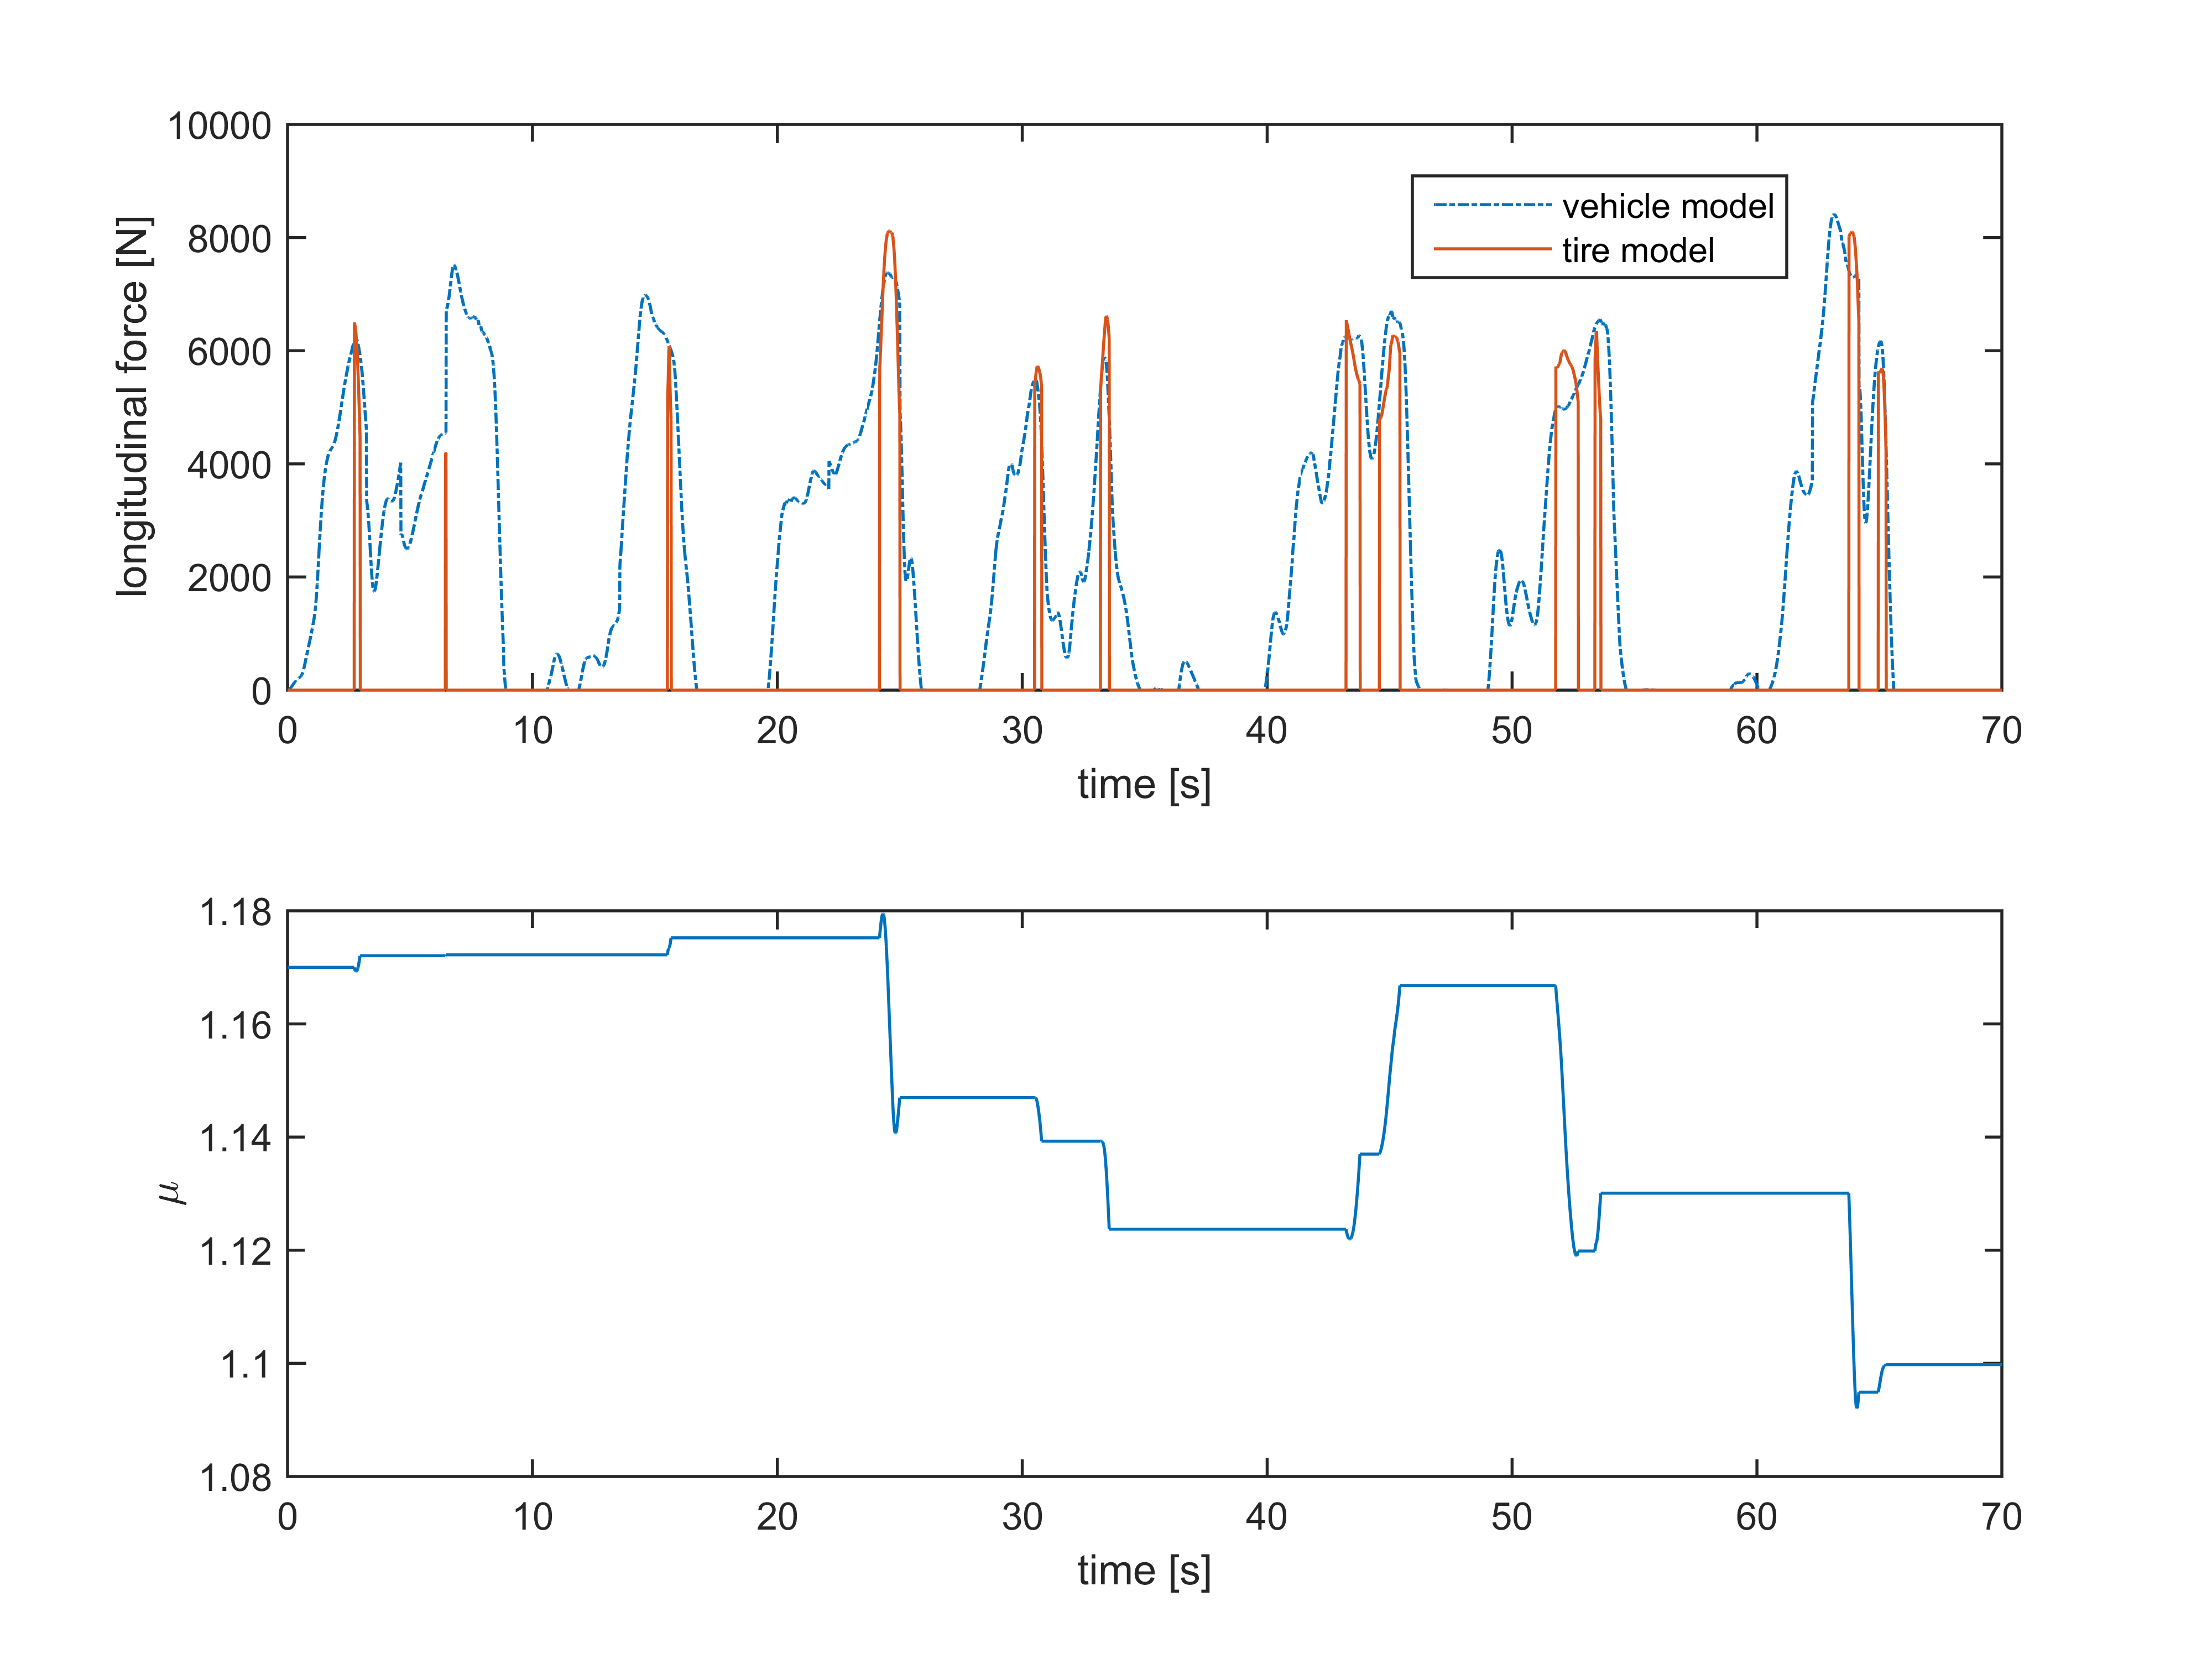
\includegraphics[width=1.0\textwidth]{Pictures/force_mue_blot_race_bb}
	\caption {Force from the tire and vehicle model and the estimated $ \mu $ for a driving sequence on wet asphalt with summer tires.}
	\label{force_mue_blot_race_bb}
\end{figure}

The normalized force per slip ratio for the dry and wet acceleration runs respectively are seen in Figure \ref{slip_kraft_blot_och_torr}. The first subplot corresponds to dry asphalt and the second subplot to wet asphalt, where the dashed line in the two subplots are exactly the same tire model parameters. The figure shows that the longitudinal force per slip ratio does not decreased when accelerating is done on wet asphalt.

\begin{figure}[h]
	\centering
	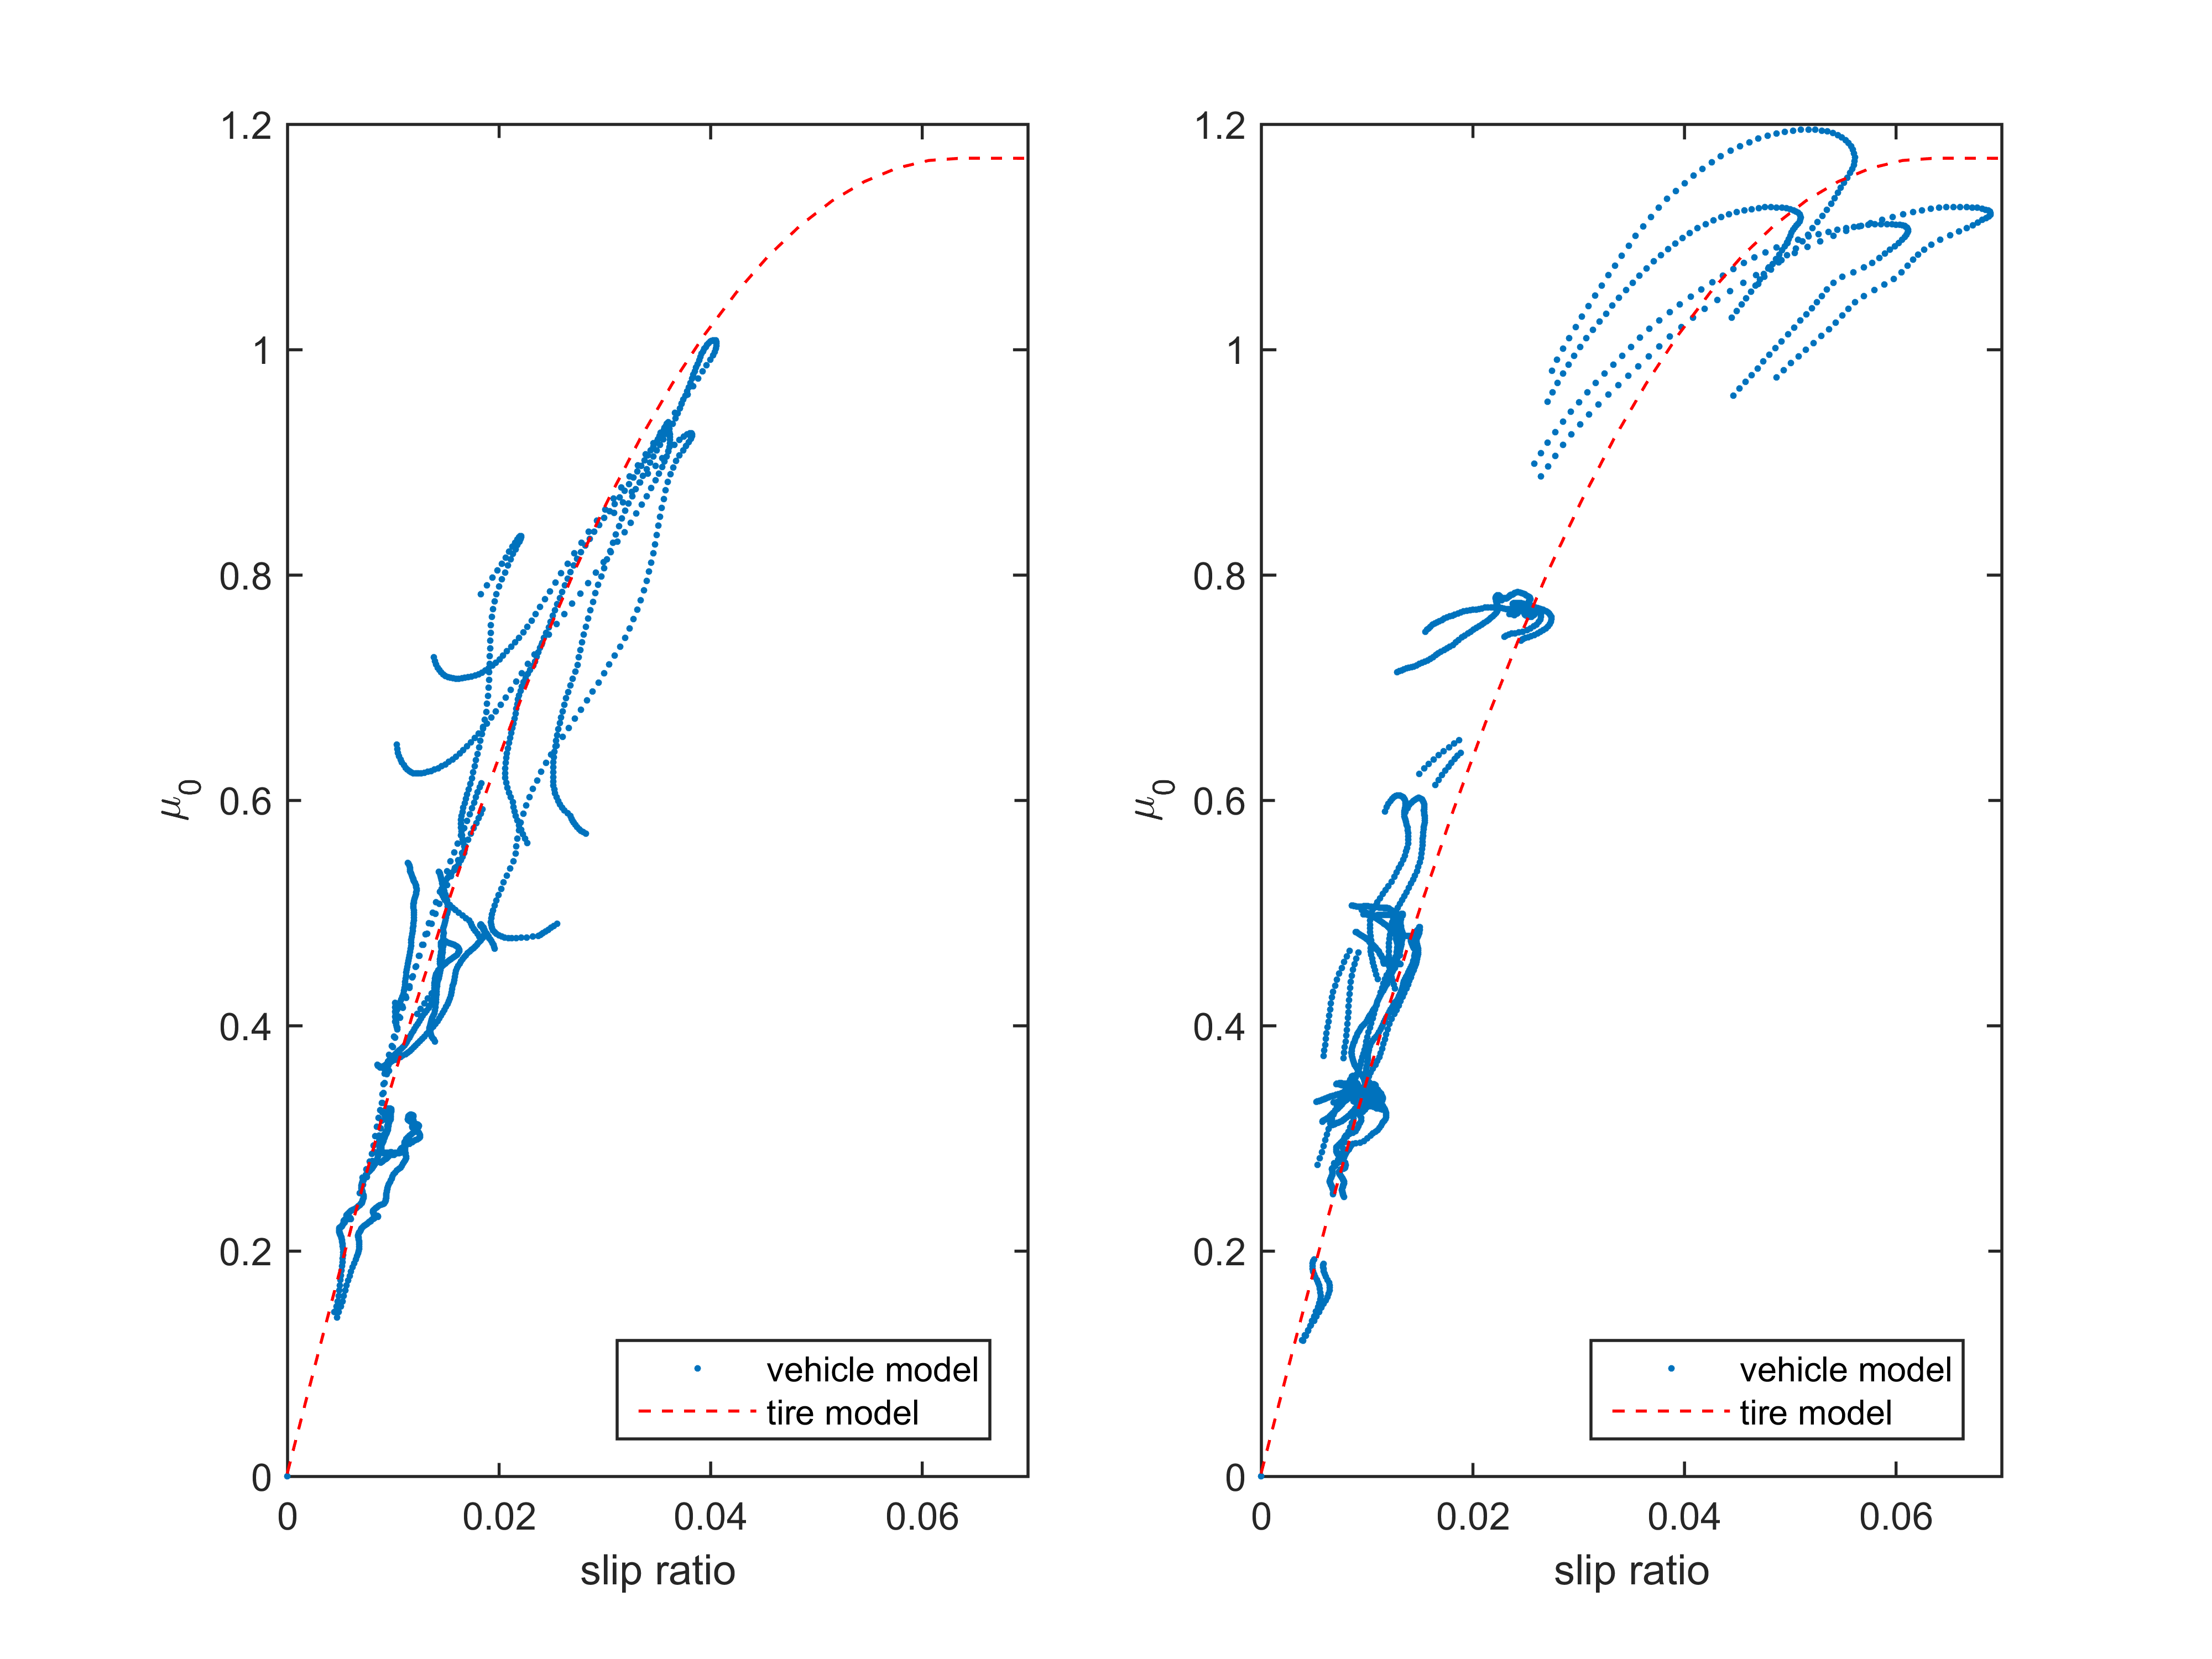
\includegraphics[width=1.0\textwidth]{Pictures/slip_kraft_blot_och_torr}
	\caption {Normalized force per slip ratio. Subplot one for dry asphalt and subplot two for wet asphalt.}
	\label{slip_kraft_blot_och_torr}
\end{figure} % Experiment 2

%\chapter{Discussion}

\section{Future work}

test with different tires! % Results and Discussion

%\chapter{Conclusion}

The work done in this report has focused as much as possible on having a solution that works in real life situations, rather than having a model that works perfectly during simulated testing. 

\section{Tire model parameters}
One of the larger insights acquire was that the difference between tire sets had a much bigger impact than what was expected. It was first believed that most tires had the force peak at similar slip ratio values, but after extensive testing this was found not to be true. Therefore the tire model needed to be extended to handle both different tires and road conditions. However, test driving have only been performed with two different sets of tires which of course restricts the possibilities to create a friction coefficient estimator that works for all tires. It's believed that the tire selector that has been developed can easily be extended to handle all kinds of tires but this requires a lot more test data from test driving with different kinds of tires and road conditions.

The estimator in whole could also be extended with several modules to enable better estimation of the friction coefficient. Methods to estimate $ V_{y} $ (lateral velocity) and $ \alpha $ (slip angle) could greatly improve estimation of the vehicle states. This would further on improve the reliability of vehicle and tire models.

\section{CAN signals used}
A goal with this report was to use signals that exist on most new vehicles of today, rather than using parameters that need new sensors or are hard to approximate. The CAN signals used in this report to approximate the friction was:
\begin{itemize}
	\item wheel speed x4
	\item engine torque
	\item lateral acceleration
	\item gear
	\item steering wheel angle
	\item FXD-moment
\end{itemize}
Besides this, static parameters associated with the Golf GTI was used.  
 % Conclusion

%% ----------------------------------------------------------------
% Now begin the Appendices, including them as separate files

\addtocontents{toc}{\vspace{2em}} % Add a gap in the Contents, for aesthetics

\appendix % Cue to tell LaTeX that the following 'chapters' are Appendices

\chapter{An Appendix}

Appendix text!	% Appendix Title

%\input{Appendices/AppendixB} % Appendix Title

%\input{Appendices/AppendixC} % Appendix Title

\addtocontents{toc}{\vspace{2em}}  % Add a gap in the Contents, for aesthetics
\backmatter

%% ----------------------------------------------------------------
\label{Bibliography}
\lhead{\emph{Bibliography}}  % Change the left side page header to "Bibliography"
\bibliographystyle{unsrtnat}  % Use the "unsrtnat" BibTeX style for formatting the Bibliography
\bibliography{Bibliography}  % The references (bibliography) information are stored in the file named "Bibliography.bib"

\end{document}  % The End
%% ----------------------------------------------------------------